% \usepackage[margin=40pt]{geometry}
% \documentclass{report}
\documentclass{book}

\usepackage[paperwidth=5.7in, paperheight=8.55in, margin=1.25cm]{geometry}
\setlength{\footskip}{\dimexpr\footskip-.3cm\relax}
\usepackage{hyperref}
\hypersetup{hidelinks}
\usepackage{xurl}
\usepackage{tocloft}
\usepackage{titletoc}
\usepackage{etoolbox}
\usepackage{multicol}
\usepackage{fontspec}
\usepackage{dsfont}
\usepackage{microtype}
\usepackage[english]{babel}
\usepackage[T1]{fontenc}
\usepackage{graphicx} 
\usepackage{wrapfig}
\usepackage{enumitem}
\usepackage{anyfontsize}
\usepackage{amsmath,amssymb}
\usepackage{tikz,tikz-layers}
\usepackage{float} 
\usepackage{subcaption}
\usepackage{caption}
\usepackage{multirow}
\usepackage{array}       
\usepackage{rotating}  

\usetikzlibrary{calc,positioning,fit}

% strenghts and weakness colors
\definecolor{mygreen}{HTML}{edf7ec}
\definecolor{myred}{HTML}{fbecec}

% chapters colors
\definecolor{cyanlight}{HTML}{d3f9ff}
\definecolor{purplelight}{HTML}{b7a1d0}
\definecolor{orangelight}{HTML}{ffecc6}
\definecolor{corallight}{HTML}{FFDEDE}
\definecolor{mintlight}{HTML}{CAFFC4}

\definecolor{cyanhard}{HTML}{9CF2FF}
\definecolor{purplehard}{HTML}{A97ADE}
\definecolor{orangehard}{HTML}{FFD689}
\definecolor{coralhard}{HTML}{FFA5A5}
\definecolor{minthard}{HTML}{A1FF98}

% formula colors
\definecolor{nmlpurple}{HTML}{3B0280}
\definecolor{nmlcyan}{HTML}{00C8E5}
\definecolor{nmlred}{HTML}{DD4040}
\definecolor{nmlgreen}{HTML}{4EB046}
\definecolor{nmlyellow}{HTML}{E1BC29}



\setsansfont{Lato}[
    Path=./fonts/LatoFont/,
    % Scale=0.9,
    Extension = .ttf,
    UprightFont=*-Regular,
    BoldFont=*-Bold,
    ItalicFont=*-Italic,
    BoldItalicFont=*-BoldItalic
    ]

\setmainfont{Rubik}[
    Path=./fonts/RubikFont/,
    % Scale=0.9,
    Extension = .ttf,
    UprightFont=*-Regular,
    BoldFont=*-SemiBold,
    ItalicFont=*-Italic,
    BoldItalicFont=*-BoldItalic
    ]

\setmonofont{PlayfairDisplay}[
    Path=./fonts/PlayFairFont/,
    % Scale=0.85,
    Extension = .ttf,
    UprightFont=*-Regular,
    BoldFont=*-Bold,
    ItalicFont=*-Italic,
    BoldItalicFont=*-BoldItalic
    ]

%============================================================================
\usepackage{fancyhdr}

% Redefine \section to center the title without number
\makeatletter
\renewcommand\section{\@startsection{section}{1}{\z@}%
  {-3.5ex \@plus -1ex \@minus -.2ex}%
  {0.3ex \@plus.2ex}%
  {\Large\bfseries\centering}}
\makeatother

% Redefine \subsection to center the title without number
\makeatletter
\renewcommand\subsection{\@startsection{subsection}{2}{\z@}%
  {-0.25ex\@plus -1ex \@minus -.2ex}%
  {1.5ex \@plus .2ex}%
  {\large\centering}}
\makeatother

% Remove visible section numbering but keep it in the .aux file for references
\setcounter{secnumdepth}{0}

% Define commands to store chapter, section title and number
\newcommand{\chaptertitle}{}
\newcommand{\sectiontitle}{}

% ---------------------------------------------------------------------------
% Chapter openers and the table of contents
% ---------------------------------------------------------------------------
% A small colored square that marks each chapter in the table of contents
% the square before a chapter title: the chapter's sidebar color, sitting on the baseline at cap height
\newcommand{\tocsquare}[1]{{\color{#1}\rule{0.7em}{0.7em}}\hspace{0.55em}}
\newcommand{\tocmark}[1]{%
    \ifstrequal{#1}{cyanaccent}{\tocsquare{cyanhard}}{%
    \ifstrequal{#1}{purpleaccent}{\tocsquare{purplehard}}{%
    \ifstrequal{#1}{orangeaccent}{\tocsquare{orangehard}}{%
    \ifstrequal{#1}{coralaccent}{\tocsquare{coralhard}}{%
    \ifstrequal{#1}{mintaccent}{\tocsquare{minthard}}{\tocsquare{#1}}}}}}}

% Table of contents styling (tocloft)
\renewcommand{\cfttoctitlefont}{\huge\bfseries}
\renewcommand{\cftaftertoctitle}{\par\vspace{1.5ex}}
\setlength{\cftbeforechapskip}{1.1em}
\renewcommand{\cftchapfont}{\large\bfseries}
\renewcommand{\cftchappagefont}{\large\bfseries}
\renewcommand{\cftchapleader}{\hfill}
\setlength{\cftchapnumwidth}{0pt}
\setlength{\cftsecindent}{1.4em}
\setlength{\cftsecnumwidth}{0pt}
\setlength{\cftbeforesecskip}{1.5pt}
\renewcommand{\cftsecfont}{\normalsize}
\renewcommand{\cftsecpagefont}{\normalsize}
\renewcommand{\cftsecdotsep}{2.5}

% Partial table of contents printed on each chapter opener (titletoc)
\titlecontents{lsection}[0em]{\normalsize}{}{}{\titlerule*[0.7pc]{.}\contentspage}[\vspace{1.5pt}]

% \chapteropener{Title}{band color}{accent color}{intro paragraphs}{list heading or empty}
\newcommand{\chapteropener}[5]{%
    \clearpage
    \refstepcounter{chapter}%
    \thispagestyle{empty}%
    \addcontentsline{toc}{chapter}{\texorpdfstring{\protect\tocmark{#3}}{}#1}%
    \renewcommand{\chaptertitle}{#1}%
    \startcontents[chapters]%
    \noindent\begin{tikzpicture}[remember picture, overlay]
        \fill[#2] (current page.north west) rectangle ([yshift=-5.6cm]current page.north east);
        \node[anchor=north west, inner sep=0pt] at ([xshift=1.25cm, yshift=-1.1cm]current page.north west)
            {\color{#3}\fontsize{58}{58}\selectfont\bfseries\thechapter};
        \node[anchor=south west, inner sep=0pt, text width=\textwidth] at ([xshift=1.25cm, yshift=-4.9cm]current page.north west)
            {\Huge\bfseries #1};
    \end{tikzpicture}\par\nointerlineskip
    \vspace*{\dimexpr 5.0cm - \baselineskip\relax}
    \noindent #4\par
    \ifblank{#5}{}{%
        \vspace{1.2em}
        {\large\bfseries #5}\par\vspace{4pt}
        {\setlength{\parskip}{0pt}\setlength{\columnsep}{1.6em}%
         \begin{multicols}{2}\raggedcolumns
         \printcontents[chapters]{l}{1}{\setcounter{tocdepth}{1}}%
         \end{multicols}}%
    }%
    \clearpage
}

% Legacy chapter command (title page only); chapters now use \chapteropener
\renewcommand{\chapter}[1]{%
    \refstepcounter{chapter}% Increment the chapter counter
    \clearpage
    \thispagestyle{empty}
    \addcontentsline{toc}{chapter}{#1}%
    \vspace*{\fill}
    {\centering\huge\bfseries #1\par}
    \vspace*{\fill}
    \clearpage
    \renewcommand{\chaptertitle}{#1}%
}

% Redefine \section to update the mark and store the title
\let\oldsection\section
\renewcommand{\section}[1]{%
    \refstepcounter{section}% Increment the section counter
    \oldsection{#1}%
    \markboth{#1}{#1}% Store only title in both marks
    \renewcommand{\sectiontitle}{#1}% Store the title for use in the style
}

\fancypagestyle{regressionstyle}{
    \fancyhf{} % Clear all header and footer fields
    % \fancyfoot[L]{\color{black!40}Daily metrics at nannyml.com/metrics} % Bottom left
    \fancyfoot[R]{\thesection\ \chaptertitle: \sectiontitle} % Bottom right, includes chapter.section number, chapter title, and section title
    \renewcommand{\headrulewidth}{0pt} % Remove header line
    \renewcommand{\footrulewidth}{0pt} % Remove footer line if undesired
    \tikz[overlay,remember picture]
    {
    \node[inner sep=0pt,outer sep=0pt,minimum width=.7cm, minimum height=\paperheight, anchor=north west, fill=cyanlight] (a) at (current page.north west) {};
    \node[anchor=east, rotate=90, xshift=-.5cm] at (a.north) 
    {
    \chaptertitle\ -- \sectiontitle % Chapter and section title here
    }; 
    }
}


\fancypagestyle{classificationstyle}{
    \fancyhf{} % Clear all header and footer fields
    % \fancyfoot[L]{\color{black!40}Daily metrics at nannyml.com/metrics} % Bottom left
    \fancyfoot[R]{\thesection\ \chaptertitle: \sectiontitle} % Bottom right, includes chapter.section number, chapter title, and section title
    \renewcommand{\headrulewidth}{0pt} % Remove header line
    % \renewcommand{\footrulewidth}{0pt} % Remove footer line if undesired
    \tikz[overlay,remember picture]
    {
    \node[inner sep=0pt,outer sep=0pt,minimum width=.7cm, minimum height=\paperheight, anchor=north west, fill=purplelight] (a) at (current page.north west) {};
    \node[anchor=east, rotate=90, xshift=-.5cm] at (a.north) 
    {
    \chaptertitle\ -- \sectiontitle % Chapter and section title here
    }; 
    }
}

\fancypagestyle{clusteringstyle}{
    \fancyhf{} % Clear all header and footer fields
    % \fancyfoot[L]{\color{black!40}Daily metrics at nannyml.com/metrics} % Bottom left
    \fancyfoot[R]{\thesection\ \chaptertitle: \sectiontitle} % Bottom right, includes chapter.section number, chapter title, and section title
    \renewcommand{\headrulewidth}{0pt} % Remove header line
    % \renewcommand{\footrulewidth}{0pt} % Remove footer line if undesired
    \tikz[overlay,remember picture]
    {
    \node[inner sep=0pt,outer sep=0pt,minimum width=.7cm, minimum height=\paperheight, anchor=north west, fill=orangelight] (a) at (current page.north west) {};
    \node[anchor=east, rotate=90, xshift=-.5cm] at (a.north) 
    {
    \chaptertitle\ -- \sectiontitle % Chapter and section title here
    }; 
    }
}

\fancypagestyle{rankingstyle}{
    \fancyhf{} % Clear all header and footer fields
    % \fancyfoot[L]{\color{black!40}Daily metrics at nannyml.com/metrics} % Bottom left
    \fancyfoot[R]{\thesection\ \chaptertitle: \sectiontitle} % Bottom right, includes chapter.section number, chapter title, and section title
    \renewcommand{\headrulewidth}{0pt} % Remove header line
    % \renewcommand{\footrulewidth}{0pt} % Remove footer line if undesired
    \tikz[overlay,remember picture]
    {
    \node[inner sep=0pt,outer sep=0pt,minimum width=.7cm, minimum height=\paperheight, anchor=north west, fill=corallight] (a) at (current page.north west) {};
    \node[anchor=east, rotate=90, xshift=-.5cm] at (a.north) 
    {
    \chaptertitle\ -- \sectiontitle % Chapter and section title here
    }; 
    }
}

\fancypagestyle{cvstyle}{
    \fancyhf{} % Clear all header and footer fields
    % \fancyfoot[L]{\color{black!40}Daily metrics at nannyml.com/metrics} % Bottom left
    \fancyfoot[R]{\thesection\ \chaptertitle: \sectiontitle} % Bottom right, includes chapter.section number, chapter title, and section title
    \renewcommand{\headrulewidth}{0pt} % Remove header line
    % \renewcommand{\footrulewidth}{0pt} % Remove footer line if undesired
    \tikz[overlay,remember picture]
    {
    \node[inner sep=0pt,outer sep=0pt,minimum width=.7cm, minimum height=\paperheight, anchor=north west, fill=mintlight] (a) at (current page.north west) {};
    \node[anchor=east, rotate=90, xshift=-.5cm] at (a.north) 
    {
    \chaptertitle\ -- \sectiontitle % Chapter and section title here
    }; 
    }
}

\fancypagestyle{nlpstyle}{
    \fancyhf{} % Clear all header and footer fields
    % \fancyfoot[L]{\color{black!40}Daily metrics at nannyml.com/metrics} % Bottom left
    \fancyfoot[R]{\thesection\ \chaptertitle: \sectiontitle} % Bottom right, includes chapter.section number, chapter title, and section title
    \renewcommand{\headrulewidth}{0pt} % Remove header line
    % \renewcommand{\footrulewidth}{0pt} % Remove footer line if undesired
    \tikz[overlay,remember picture]
    {
    \node[inner sep=0pt,outer sep=0pt,minimum width=.7cm, minimum height=\paperheight, anchor=north west, fill=cyanhard] (a) at (current page.north west) {};
    \node[anchor=east, rotate=90, xshift=-.5cm] at (a.north) 
    {
    \chaptertitle\ -- \sectiontitle % Chapter and section title here
    }; 
    }
}

\fancypagestyle{genaistyle}{
    \fancyhf{} % Clear all header and footer fields
    % \fancyfoot[L]{\color{black!40}Daily metrics at nannyml.com/metrics} % Bottom left
    \fancyfoot[R]{\thesection\ \chaptertitle: \sectiontitle} % Bottom right, includes chapter.section number, chapter title, and section title
    \renewcommand{\headrulewidth}{0pt} % Remove header line
    % \renewcommand{\footrulewidth}{0pt} % Remove footer line if undesired
    \tikz[overlay,remember picture]
    {
    \node[inner sep=0pt,outer sep=0pt,minimum width=.7cm, minimum height=\paperheight, anchor=north west, fill=purplehard] (a) at (current page.north west) {};
    \node[anchor=east, rotate=90, xshift=-.5cm] at (a.north) 
    {
    \chaptertitle\ -- \sectiontitle % Chapter and section title here
    }; 
    }
}

\fancypagestyle{probabilisticstyle}{
    \fancyhf{} % Clear all header and footer fields
    % \fancyfoot[L]{\color{black!40}Daily metrics at nannyml.com/metrics} % Bottom left
    \fancyfoot[R]{\thesection\ \chaptertitle: \sectiontitle} % Bottom right, includes chapter.section number, chapter title, and section title
    \renewcommand{\headrulewidth}{0pt} % Remove header line
    % \renewcommand{\footrulewidth}{0pt} % Remove footer line if undesired
    \tikz[overlay,remember picture]
    {
    \node[inner sep=0pt,outer sep=0pt,minimum width=.7cm, minimum height=\paperheight, anchor=north west, fill=orangehard] (a) at (current page.north west) {};
    \node[anchor=east, rotate=90, xshift=-.5cm] at (a.north) 
    {
    \chaptertitle\ -- \sectiontitle % Chapter and section title here
    }; 
    }
}

\fancypagestyle{biasfairnesstyle}{
    \fancyhf{} % Clear all header and footer fields
    % \fancyfoot[L]{\color{black!40}Daily metrics at nannyml.com/metrics} % Bottom left
    \fancyfoot[R]{\thesection\ \chaptertitle: \sectiontitle} % Bottom right, includes chapter.section number, chapter title, and section title
    \renewcommand{\headrulewidth}{0pt} % Remove header line
    % \renewcommand{\footrulewidth}{0pt} % Remove footer line if undesired
    \tikz[overlay,remember picture]
    {
    \node[inner sep=0pt,outer sep=0pt,minimum width=.7cm, minimum height=\paperheight, anchor=north west, fill=coralhard] (a) at (current page.north west) {};
    \node[anchor=east, rotate=90, xshift=-.5cm] at (a.north) 
    {
    \chaptertitle\ -- \sectiontitle % Chapter and section title here
    }; 
    }
}

\fancypagestyle{observabilitystyle}{
    \fancyhf{} % Clear all header and footer fields
    % \fancyfoot[L]{\color{black!40}Daily metrics at nannyml.com/metrics} % Bottom left
    \fancyfoot[R]{\thesection\ \chaptertitle: \sectiontitle} % Bottom right, includes chapter.section number, chapter title, and section title
    \renewcommand{\headrulewidth}{0pt} % Remove header line
    % \renewcommand{\footrulewidth}{0pt} % Remove footer line if undesired
    \tikz[overlay,remember picture]
    {
    \node[inner sep=0pt,outer sep=0pt,minimum width=.7cm, minimum height=\paperheight, anchor=north west, fill=minthard] (a) at (current page.north west) {};
    \node[anchor=east, rotate=90, xshift=-.5cm] at (a.north) 
    {
    \chaptertitle\ -- \sectiontitle % Chapter and section title here
    }; 
    }
}

\fancypagestyle{customstyle}{
    \fancyhf{} % Clear all header and footer fields
    % \fancyfoot[L]{\color{black!40}Daily metrics at nannyml.com/metrics} % Bottom left
    \fancyfoot[R]{\thesection\ \chaptertitle: \sectiontitle} % Bottom right, includes chapter.section number, chapter title, and section title
    \renewcommand{\headrulewidth}{0pt} % Remove header line
    \renewcommand{\footrulewidth}{0pt} % Remove footer line if undesired
}

%============================================================================



\setlength{\parindent}{0pt}
\setlength{\parskip}{8pt}
\raggedbottom


\newcommand{\coloredboxes}[2]{
\tikz[every node/.style={outer sep=0pt, inner sep=0pt, align=left}] {
\node[ minimum width=.5\textwidth, minimum height=1cm, label={[yshift=-7.5mm]above:\strut\textbf{Strengths}}] (a) {
\\[.7cm]
\parbox{.45\textwidth}{
\begin{itemize}[left=0pt, label={\textcolor{teal!60!green!60}{$\bullet$}}]
    #1
\end{itemize}
}

};

\path let \p1 = (a.north), \p2 = (a.south) in
node[ minimum width=.5\textwidth, minimum height=\y1-\y2, 
label={[yshift=-7.5mm]above:\strut\textbf{Weaknesses}}, anchor=north west] (b) at (a.north east) {
\\[.7cm]
\parbox{.45\textwidth}{
\begin{itemize}[left=0pt, label={\textcolor{red!80!black!60}{$\bullet$}}]
    #2
\end{itemize}
}

};

\begin{scope}[on behind layer]
\fill[mygreen] (current bounding box.north)--($(current bounding box.north west)+(.4,0)$) to[bend right=45] ($(current bounding box.north west)+(0,-.4)$)--($(current bounding box.south west)+(0,.4)$) to[bend right=45] ($(current bounding box.south west)+(.4,0)$)--(current bounding box.south)--cycle;    
\end{scope}

\begin{scope}[on behind layer]
\fill[myred] (current bounding box.north)--($(current bounding box.north east)+(-.4,0)$) to[bend left=45] ($(current bounding box.north east)+(0,-.4)$)--($(current bounding box.south east)+(0,.4)$) to[bend left=45] ($(current bounding box.south east)+(-.4,0)$)--(current bounding box.south)--cycle;    
\end{scope}
}
}



\newcommand{\orangebox}[2]{
{\bigskip\tikz[]{
\node[outer sep=0pt, inner ysep=.4cm, minimum width=\textwidth, fill=orangelight, rounded corners=2mm, align=left, text width=\textwidth-1cm] {
\textit{\ttfamily #1}\\[2mm]
#2
};
}}
}

\usepackage{array}
\usepackage{xcolor}
\usepackage{colortbl}
\usepackage[table]{xcolor}

% accent colors used on chapter openers (a darker tone of each chapter's sidebar color)
\colorlet{cyanaccent}{cyanhard!45!black}
\colorlet{purpleaccent}{purplehard!60!black}
\colorlet{orangeaccent}{orangehard!55!black}
\colorlet{coralaccent}{coralhard!55!black}
\colorlet{mintaccent}{minthard!45!black}

% ---------- Decision maps: one page per chapter, right after the opener ----------
% A printed key, like the identification keys in a field guide: a question in
% bold, its possible answers indented beneath it, and the metric that answer
% leads to on the right with its page number.  Nested questions indent further.
\colorlet{mapband}{cyanlight}
\colorlet{mapaccent}{cyanaccent}
\newcommand{\maptitle}{Which metric?}
\fancypagestyle{mapstyle}{
    \fancyhf{}
    \fancyfoot[R]{\chaptertitle: \maptitle}
    \renewcommand{\headrulewidth}{0pt}
    \renewcommand{\footrulewidth}{0pt}
    \tikz[overlay,remember picture]{
        \node[inner sep=0pt,outer sep=0pt,minimum width=.7cm, minimum height=\paperheight, anchor=north west, fill=mapband] (a) at (current page.north west) {};
        \node[anchor=east, rotate=90, xshift=-.5cm] at (a.north) {\chaptertitle\ -- \maptitle};
    }
}
% a metric with its page number
\newcommand{\mref}[2]{#1~{\color{black!55}\mdseries\scriptsize\pageref{#2}}}
\newcommand{\nohyph}{\hyphenpenalty=10000 \exhyphenpenalty=10000 }
\newlength{\mapindent}\setlength{\mapindent}{1.25em}
% \begin{decisionmap}{band}{accent}{title}{subtitle} ... \end{decisionmap}
\newenvironment{decisionmap}[4]{%
    \clearpage
    \colorlet{mapband}{#1}\colorlet{mapaccent}{#2}%
    \renewcommand{\maptitle}{#3}%
    \thispagestyle{mapstyle}%
    \noindent{\color{#2}\fontsize{22}{26}\selectfont\bfseries #3}\par
    \vspace{5pt}
    {\color{black!60}\small #4\par}
    \vspace{6pt}
    \begingroup\small\setlength{\parindent}{0pt}\setlength{\parskip}{0pt}\setlength{\leftskip}{0pt}\nohyph
}{%
    \endgroup\clearpage
}
% a question (bold); the first one starts the key, nested ones follow an answer
\newcommand{\mapq}[1]{\par\vspace{8pt}{\bfseries\color{black!85}#1}\par\vspace{3pt}}
% an answer, with the metric(s) it leads to on the right; leave #2 empty when a nested question follows
% the empty \hbox keeps the dotted leader alive when the metric wraps to its own line, so it still ends at the right margin
\newcommand{\mapa}[2]{\par{\color{black!70}#1}\ifblank{#2}{}{\hspace{0.4em}\hbox{}\nobreak{\color{black!25}\leaders\hbox to 0.55em{\hss.\hss}\hfill}\nobreak\hspace{0.3em}\mbox{\bfseries\color{black!85}#2}}\par\vspace{3pt}}
% nesting: everything inside is indented one level
\newenvironment{mapsub}{\par\addtolength{\leftskip}{\mapindent}}{\par\addtolength{\leftskip}{-\mapindent}}
\newcommand{\mapnotes}[1]{\par\vspace{14pt}{\color{black!60}\footnotesize\setlength{\parskip}{3pt}#1\par}}

\begin{document}
\pagestyle{customstyle}

% ---------- title page ----------
\begin{titlepage}
    \thispagestyle{empty}
    \begin{tikzpicture}[remember picture, overlay]
        \fill[cyanlight] (current page.north west) rectangle ([yshift=-0.58\paperheight]current page.north east);
        \node[anchor=south west, inner sep=0pt, text width=\textwidth] at ([xshift=1.25cm, yshift=-0.58\paperheight+1.4cm]current page.north west)
            {\fontsize{34}{40}\selectfont\bfseries The Little Book of\\[2pt] ML Metrics};
        \node[anchor=north west, inner sep=0pt, text width=\textwidth] at ([xshift=1.25cm, yshift=-0.58\paperheight-1.2cm]current page.north west)
            {\Large What every metric measures, when to use it, and where it fails.\\[1.6em]
             \normalsize\color{black!60}Regression, classification, clustering, ranking, computer vision, NLP, GenAI,
             probabilistic performance estimation, bias and fairness, and data observability.};
        \node[anchor=south west, inner sep=0pt] at ([xshift=1.25cm, yshift=1.4cm]current page.south west)
            {\large\bfseries NannyML};
    \end{tikzpicture}
\end{titlepage}

\setcounter{tocdepth}{1}  % 1 includes chapters and sections
\pagestyle{plain}
\tableofcontents
\clearpage
\pagestyle{customstyle}
\chapteropener{Introduction}{cyanlight}{cyanaccent}{%
% Santiago writes the opening text himself (review note, 2026-09-06). Left blank on purpose.
}{}

\clearpage
\thispagestyle{customstyle}
\section{Who this is for}

You build models, or you keep an eye on models that are already running, and you know what a confusion matrix and a residual are. That is
all we assume. What you probably don't have is a clear answer to the question that comes up in every model review: which number should
we be looking at, and what does it hide?

That is the whole point of this book. Each metric gets two pages. Not a lecture, just the things you'd want a colleague to tell you
before you pick it: what it measures, when it is the right choice, and where it will fool you.

\section{How to read a metric page}

Every metric follows the same layout, so once you've read one you know where to look on all the others.

\textbf{Page one} is the definition. A short paragraph on what the number means in practice, then the formula with every symbol
labeled, then how to read the value: the range, what counts as good, what counts as bad. After that, when to use it and when not to, and
two boxes side by side: strengths on the left, weaknesses on the right. We tried to make every bullet concrete. ``Sensitive to outliers''
tells you nothing; ``one prediction off by 100 counts as much as 99 predictions off by 1'' does.

\textbf{Page two} is the metric in action. The figure shows how the metric turns inputs into a score, and every number on it comes
from the data it draws. The caption tells you how to read it. Then a ``did you know'' box with one fact that changes how you think
about the metric, and a short note on related metrics: which neighbors to consider, and what it means when two of them disagree.

The data observability chapter is the exception. Its monitors are simple statistics, so each one gets a single page with a figure.

\section{The colors in the formulas}

Every symbol in a formula is colored by what it is, and the arrows spell it out:

\begin{itemize}[left=0pt]
    \item {\color{nmlcyan}\textbf{Cyan}} is the truth: targets, labels, actual values.
    \item {\color{nmlpurple}\textbf{Purple}} is what the model produced: predictions, scores, estimates.
    \item {\color{nmlred}\textbf{Red}} is a count or a size: how many samples, classes, bins or items.
    \item {\color{nmlgreen}\textbf{Green}} is a special function, like the indicator $\mathds{1}[\cdot]$.
    \item {\color{nmlyellow}\textbf{Yellow}} is something you choose: a threshold, a weight, a quantile level.
\end{itemize}

The same colors mean the same thing in every chapter.

\section{Picking a metric}

Three questions settle most of it.

\textbf{What does a mistake cost?} If a big miss hurts much more than a small one, you want squared errors. If a false alarm and a
missed case cost different amounts, you want precision or recall rather than accuracy, or the expected cost directly. If you can't say
what a mistake costs, the metric is deciding for you.

\textbf{How rare is the thing you care about?} Rare positives make accuracy and ROC AUC look great while the model misses them.
Tiny targets make percentage errors explode. Different base rates across groups make most fairness criteria impossible to satisfy at
the same time. Check the balance before you check the score.

\textbf{Who is going to read the number?} A metric in the target's own units, like MAE, is for the people who own the target. A
scale-free one, like $R^2$ or nDCG, is for comparing models across datasets. A proper scoring rule, like log loss, is for training and
calibration. One model can deserve all three, reported to different people.

Each chapter starts with a one-page key that walks through these questions for its metrics. And when two metrics that should agree
don't, the disagreement is usually the most useful thing on the page: RMSE far above MAE means a few large errors; ROC AUC high with
PR AUC low means the rare class is being missed.

\section{How the book is organized}

Chapters follow what the model outputs. Regression and classification first, since almost everyone meets those. Then clustering and
ranking, then computer vision, NLP and generative models, where the reference answer gets fuzzier and learned judges take over. The
last three chapters step back: estimating a metric before the labels arrive, checking whether the score is the same for every group,
and watching the tables that feed all of it. Every figure is generated by code in the book's repository, from the data it shows.

\include{2-regression}
\include{3-classification}
\include{4-clustering}
\chapter{Ranking}

% ---------- @K Metrics ----------
\clearpage
\thispagestyle{rankingstyle}
\section{@K Metrics}
\subsection{@K Metrics}

Most ranking metrics score the full ordering, but users rarely scroll past the first screen. The @K family restricts evaluation to the top-$K$ items, matching the slice of the ranking that actually drives engagement. Any base metric — Precision, Recall, MRR, MAP, nDCG — has an @K variant that ignores everything below rank $K$.

\begin{center}
    $\displaystyle Precision@K = \frac{|\text{relevant items in top-}K|}{K}$
\end{center}

The value of $K$ is set by the product, not the model: $K = 5$ for a mobile carousel, $K = 10$ for a search results page. Two models with identical full-ranking scores can disagree completely at small $K$, so the cutoff is part of the evaluation.

\textbf{When to use @K metrics?}

Use @K when the user sees a fixed window: search pages, feeds, carousels. Pick $K$ from the UI surface. Avoid @K when the full ordering matters downstream (re-ranking, audit) or when $K$ is itself the variable being optimized.

\coloredboxes{
    \item Matches what users actually see. $Precision@5$ on a mobile carousel directly measures the relevance of the slice the user is shown.
    \item Composable across metrics. Every base ranking metric has a clean @K variant, so a single cutoff applies across an evaluation suite.
}
{
    \item Sensitive to the choice of $K$. Precision@$5$ and Precision@$20$ can order models differently; report at several $K$ or fix $K$ from the product spec.
    \item Hard cutoff at rank $K$. An item at rank $K+1$ is treated identically to one at rank $1000$, even though it nearly made the list.
    \item Precision@$K$ has a ceiling when relevant items are scarce. With three relevant items, $Precision@10$ maxes at $0.3$ even for a perfect ranker.
}

\clearpage
\thispagestyle{customstyle}

\begin{figure*}[ht!]
    \centering
    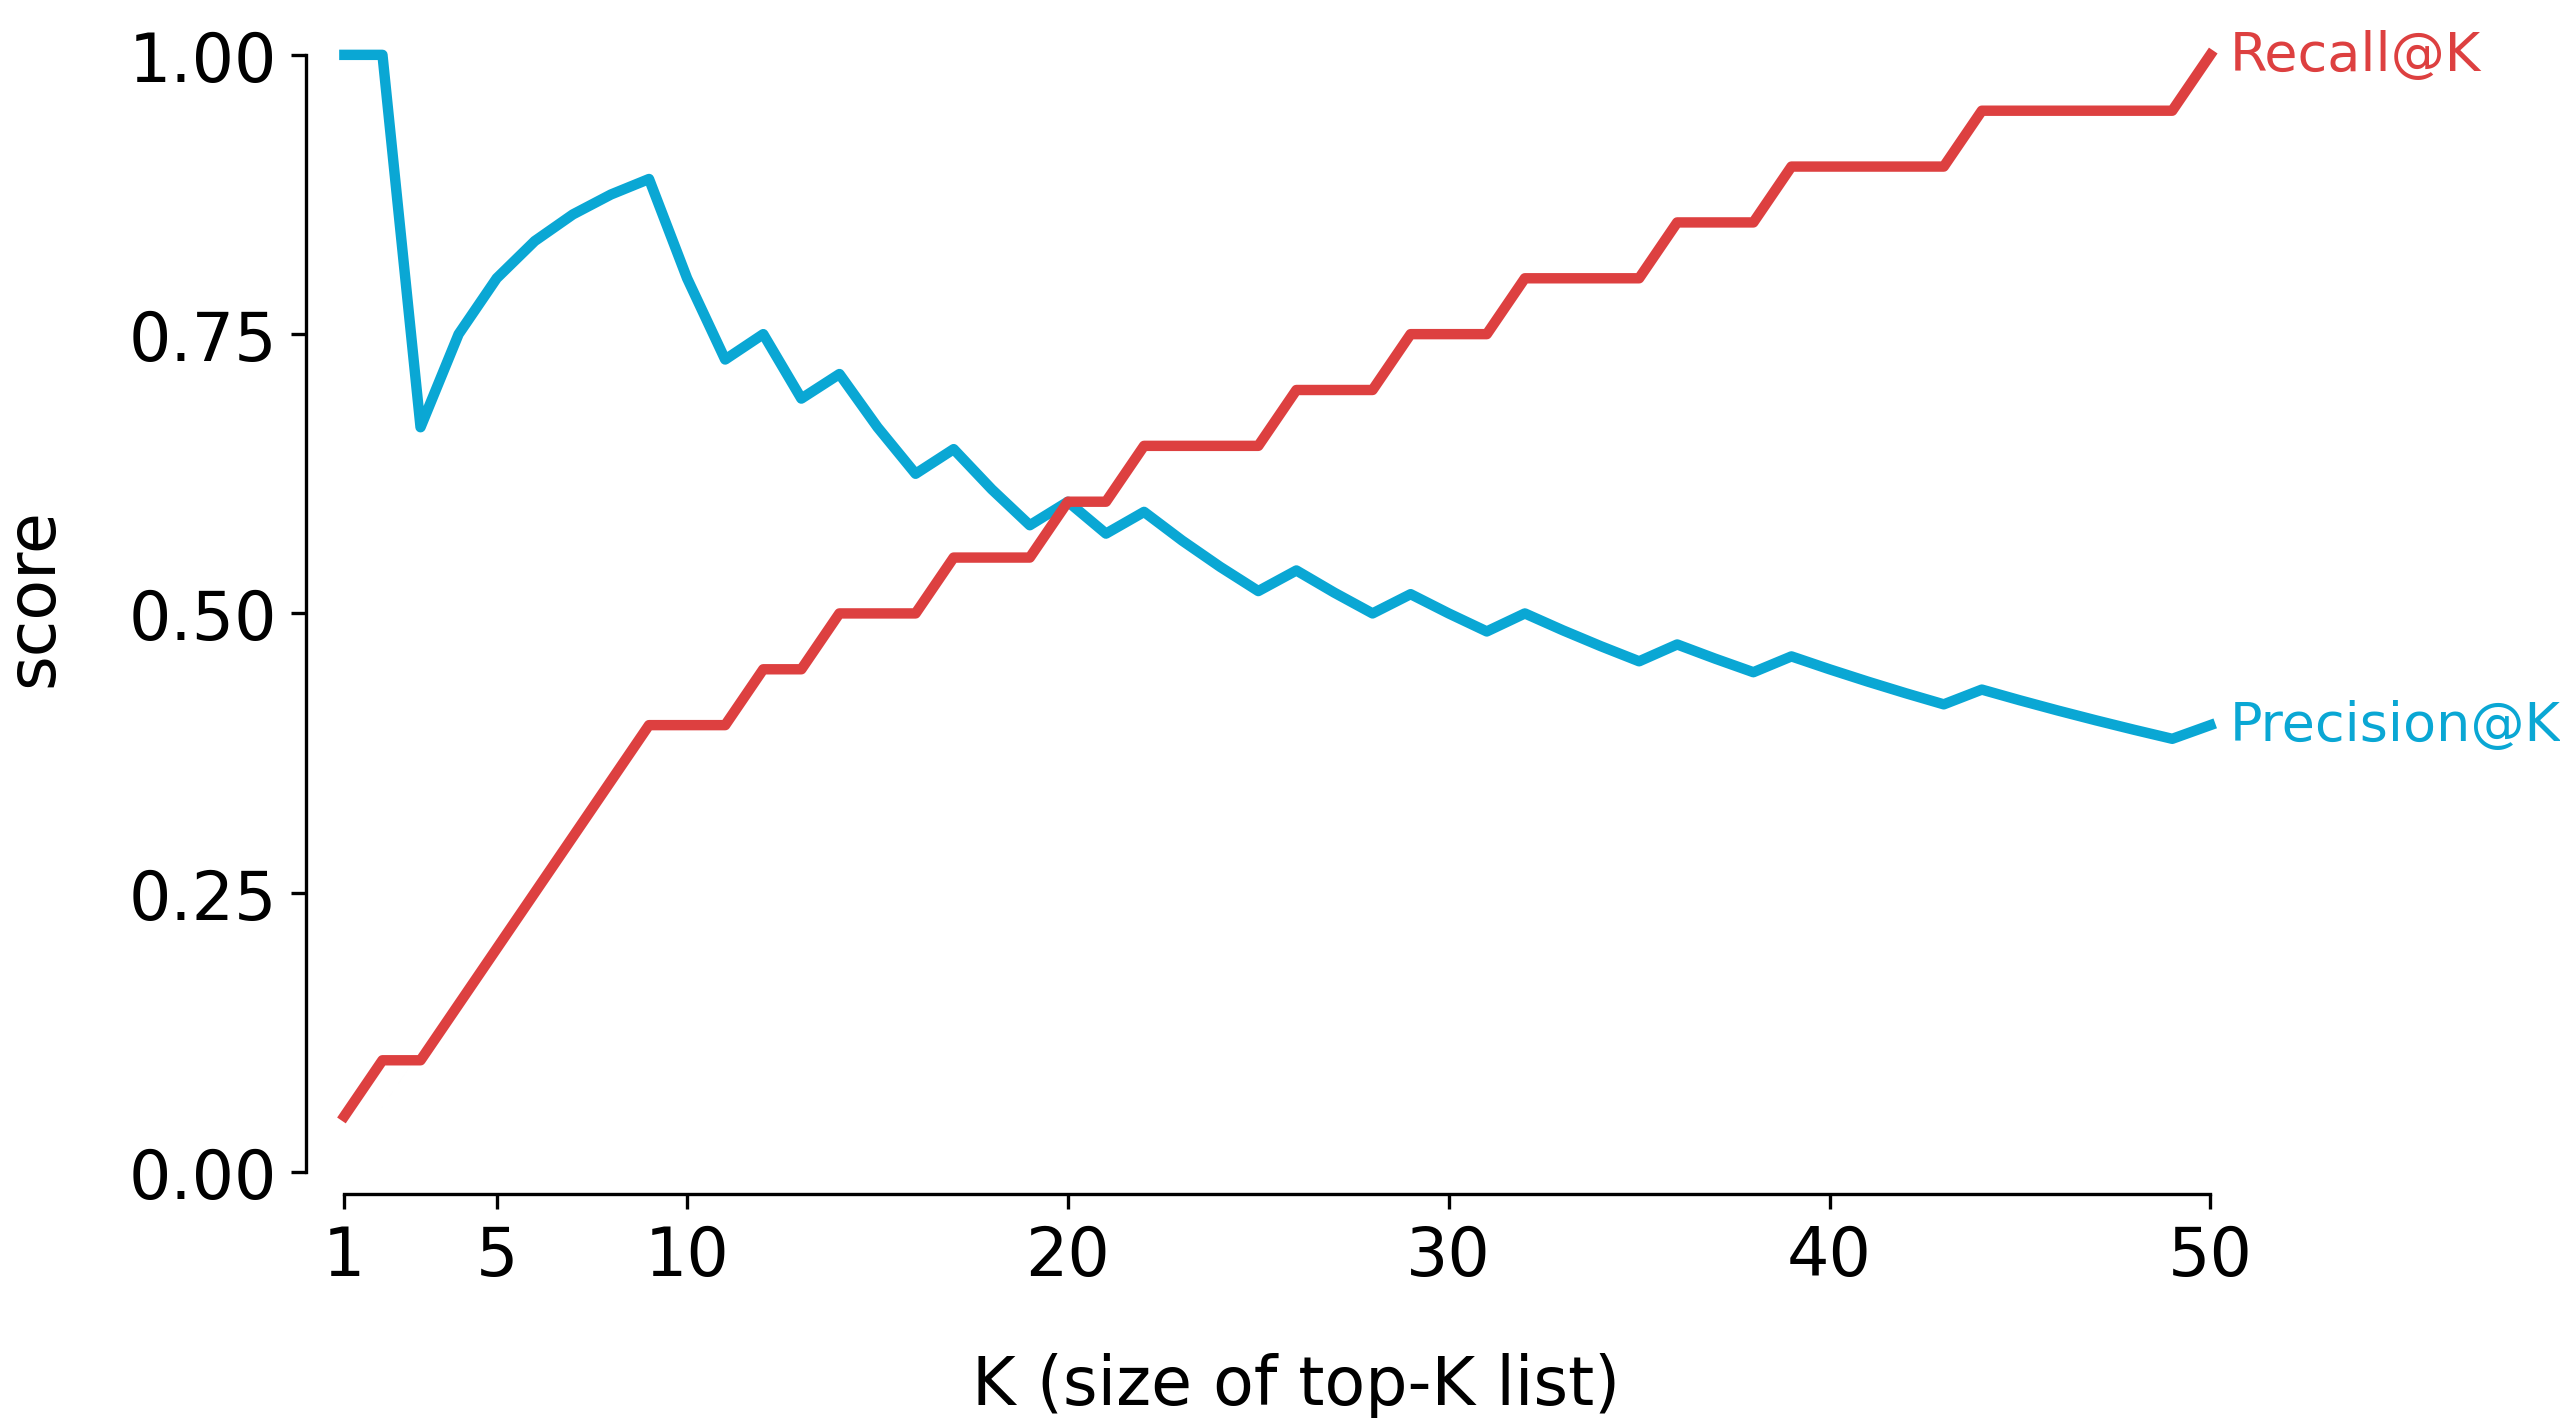
\includegraphics[width=0.85\textwidth]{figures/at_K_precision_recall.png}
\end{figure*}

\textbf{Figure.} Precision@$K$ (blue) falls and Recall@$K$ (red) rises as $K$ grows. The crossover at $K = 20$ is where both curves agree: $60\%$ of relevant items retrieved at $60\%$ precision. Picking $K$ to the left of the crossover means optimizing for a clean top of the list; to the right, for covering more of the relevant set. The shape of the two curves is the practical artifact — the exact crossover shifts with the underlying relevance distribution.

\orangebox{Did you know that...}
{The choice of $K$ is often driven by UI constraints. If a mobile app shows five cards on screen, $Precision@5$ measures exactly the value of that screen. Reporting $Precision@10$ when only five are visible measures a different product than the one users see.}

\textbf{Other related metrics}

Common @K variants include Precision@$K$, Recall@$K$, MAP@$K$, and nDCG@$K$. For a binary check of whether any relevant item appears in the top-$K$, see Hit Rate.

% ---------- Mean Reciprocal Rank ----------
\clearpage
\thispagestyle{rankingstyle}
\section{Mean Reciprocal Rank}
\subsection{MRR}

MRR scores a system on a narrow question: how high in the list is the first relevant result? Average that reciprocal across all queries and the result is MRR. The metric heavily weights the rank-$1$ result and gives little credit when the first relevant item appears at rank $5$ or $10$ — useful for tasks where users abandon the list after the first miss.

\begin{center}
    \tikz{
        \node[inner sep=2pt, font=\Large] (a) {
            {
                $\displaystyle
                MRR = \frac{1}{{\color{nmlred}|Q|}} \sum_{i=1}^{|Q|} \frac{1}{{\color{nmlcyan}rank_i}}
                $
            }
        };
        \draw[overlay,-latex,nmlred, semithick] ($(a.south)+(-0.5,0.2)$) to[bend left=15] node[pos=1, left] {number of queries} +(-1,-.5);
        \draw[overlay,-latex,nmlcyan, semithick] ($(a.north)+(2.0,-0.1)$) to[bend left=15] node[pos=1, right] {first relevant rank} +(1,.5);
    }
\end{center}

MRR lives in $[0, 1]$. A score of $1$ means the relevant item sits at rank $1$ for every query; $0.5$ means the average first-hit is at rank $2$. The decay is hyperbolic — rank $5$ scores $0.2$, rank $20$ scores $0.05$ — so anything past the first relevant item is essentially invisible.

\textbf{When to use MRR?}

Use MRR for known-item search and Q\&A: each query has one canonical answer and the task is to surface it first (``what's the capital of Belgium?''). Avoid MRR when queries have multiple relevant items of comparable value (movies, news) — MRR scores the same whether the slots after the first hit are gold or junk.

\coloredboxes{
    \item Mirrors known-item search. Users want the answer at rank $1$, and MRR penalizes anything below it.
    \item Bounded in $[0, 1]$ and averageable across queries with no normalization.
}
{
    \item Ignores items below the first hit. $[\textit{relevant, junk, junk}]$ and $[\textit{relevant, gold, gold}]$ score the same.
    \item Steep penalty for top-of-list misses. Rank $1$ to rank $2$ halves the score; rank $1$ to rank $10$ drops it by $90\%$.
    \item Inflatable with short rankings — pair MRR with Recall or coverage.
}

\clearpage

\thispagestyle{customstyle}

\begin{figure*}[ht!]
    \centering
    \includegraphics[width=0.6\textwidth]{figures/MRR_reciprocal_rank.png}
\end{figure*}

\textbf{Figure.} Each query contributes the reciprocal of its first-relevant rank to the MRR sum. The drop is fast: rank $1$ gives $1.0$, rank $2$ gives $0.5$, rank $5$ gives $0.2$. Past rank $10$ the reciprocal is small enough that it barely matters whether the relevant item appeared at rank $11$ or rank $1000$ — MRR cares almost exclusively about the top of the list.

\orangebox{Did you know that...}
{MRR is the default scorer for question-answering benchmarks like TREC-QA and Natural Questions because the task is structurally known-item: there is one right answer and the user wants it first. Swapping MRR for nDCG only changes the score on queries with multiple plausible answers — for single-answer queries the two are essentially equivalent.}

\textbf{Other related metrics}

For multi-relevant evaluation use MAP. For graded relevance (some items more relevant than others, e.g., a five-star rating system) use nDCG — it credits every relevant item with a position-discounted contribution, whereas MRR collapses the entire list to a single number from the first hit. For a binary top-$K$ check use Hit Rate.


% ---------- Mean Average Precision ----------
\clearpage
\thispagestyle{rankingstyle}
\section{Mean Average Precision}
\subsection{Mean Average Precision}

MAP rewards rankers for placing relevant items high in the list. For each query, walk down the ranking and average the precision at every position where a relevant item appears — that is the Average Precision (AP). MAP is the mean of AP across queries. A relevant item at rank $1$ contributes precision $1.0$; at rank $10$ it contributes $0.1$, so MAP collapses when relevant items are buried.

\begin{center}
    \tikz{
        \node[inner sep=2pt, font=\Large] (a) {
            {
                $\displaystyle
                MAP = \frac{1}{{\color{nmlred}|Q|}} \sum_{q=1}^{|Q|} \frac{1}{|{\color{nmlcyan}R_q}|} \sum_{k=1}^{n} {\color{nmlpurple}P(k)} \cdot {\color{nmlcyan}rel(k)}
                $
            }
        };
        \draw[overlay,-latex,nmlred, semithick] ($(a.south)+(-1.5,0.2)$) to[bend left=15] node[pos=1, left] {number of queries} +(-1,-.5);
        \draw[overlay,-latex,nmlcyan, semithick] ($(a.north)+(2.0,-0.1)$) to[bend left=15] node[pos=1, right] {relevant items} +(1,.5);
        \draw[overlay,-latex,nmlpurple, semithick] ($(a.south)+(2.5,0.3)$) to[bend left=15] node[pos=1, left] {precision at $k$} +(-1,-.5);
    }
\end{center}

MAP lives in $[0, 1]$. A perfect ranking — every relevant item ahead of every irrelevant one — scores $1$. The gap between MAP and the prevalence baseline (relevant items / list length) measures how much ordering work the model adds on top of plain retrieval.

\textbf{When to use MAP?}

Use MAP when relevance is binary, the full ranked list matters, and you want one number for precision plus order. It is the standard for binary-judgment IR benchmarks. Avoid MAP for graded relevance (use nDCG) or top-only evaluation (use MRR or Precision@$K$) — averaging across all positions lets a strong tail mask a weak top.

\coloredboxes{
    \item Captures precision and rank order in one number. A model that surfaces relevant items earlier always scores higher.
    \item Averages cleanly across queries with different numbers of relevant items — AP is already per-query normalized.
}
{
    \item Assumes binary relevance. No way to say ``item A is more relevant than item B'' the way nDCG can.
    \item Requires complete labels. If a query has five relevant items and only three are labeled, AP is biased downward.
    \item Hard to translate to a user-facing story. ``MAP $= 0.42$'' lands flat next to ``$Precision@10 = 0.6$''.
}

\clearpage
\thispagestyle{customstyle}

\begin{figure*}[ht!]
    \centering
    \includegraphics[width=0.85\textwidth]{figures/MAP_good_vs_bad.png}
\end{figure*}

\textbf{Figure.} Both rankings retrieve four relevant items. The left places them at ranks $1, 2, 3, 6$ and earns $AP = 0.92$; the right at ranks $4, 7, 9, 10$ and earns $AP = 0.32$. Same recall, very different MAP — exactly the gap MAP exists to measure.

\orangebox{Did you know that...}
{MAP became the default scorer for the TREC (Text REtrieval Conference) evaluations, which have been benchmarking information retrieval systems since 1992. The choice was deliberate: MAP credits precision at every position where a relevant item appears, so a system that surfaces the same items earlier always wins — exactly the property TREC wanted to reward across thirty years of system comparisons.}

\textbf{Other related metrics}

For graded relevance use nDCG. For top-only evaluation use MRR or Precision@$K$. AP and MAP are related as point and average: AP is the per-query score, MAP is the mean across queries.

% good resources for inpiration for visual: https://juneandrews.com/2014/12/15/mean-average-precision-isnt-so-nice/
% https://sdsawtelle.github.io/blog/output/mean-average-precision-MAP-for-recommender-systems.html

% ---------- Hit Rate ----------
\clearpage
\thispagestyle{rankingstyle}
\section{Hit Rate}
\subsection{Hit Rate}

Hit Rate answers a yes-no question per user: did the top-$K$ list contain at least one relevant item? Average that indicator across users and you have the Hit Rate of the system. It ignores how many relevant items appeared and where they were — only whether the user got something or nothing.

\begin{center}
    \tikz{
        \node[inner sep=2pt, font=\Large] (a) {
            {
                $\displaystyle
                Hit\ Rate = \frac{1}{{\color{nmlred}|U|}} \sum_{u=1}^{|U|} {\color{nmlgreen}\mathds{1}}\left(|{\color{nmlcyan}R_u} \cap {\color{nmlpurple}Top\text{-}K_u}| > 0\right)
                $
            }
        };
        \draw[overlay,-latex,nmlred, semithick] ($(a.south)+(-2.0,0.2)$) to[bend left=15] node[pos=1, left] {number of users} +(-1,-.5);
        \draw[overlay,-latex,nmlcyan, semithick] ($(a.north)+(2.0,-0.1)$) to[bend right=15] node[pos=1, left] {relevant items} +(-1,.5);
        \draw[overlay,-latex,nmlpurple, semithick] ($(a.north)+(3.5,-0.1)$) to[bend left=15] node[pos=1, right] {top-K items} +(1,.5);
    }
\end{center}

A Hit Rate of $0.72$ means $72\%$ of users got at least one relevant item in their top-$K$ list; the other $28\%$ saw nothing useful. The low bar makes Hit Rate the right metric for catching a specific failure: lists that look diverse but happen to miss every user's actual interests.

\textbf{When to use Hit Rate?}

Use Hit Rate as a floor for top-$K$ quality: ``what fraction of sessions show at least one relevant item?'' translates directly to product metrics. Avoid Hit Rate as the primary optimization target — a model can score well by recommending broadly, with no signal about whether the hit is buried in junk.

\coloredboxes{
    \item Easy to communicate. ``$72\%$ of sessions see at least one relevant item'' maps directly onto product metrics like activation or session quality.
    \item Robust to sparsity and missing labels. A single relevant item per user is enough to score.
    \item Endpoint-interpretable. $0$ means total failure; $1$ means every user is served.
}
{
    \item Position-blind. A relevant item at rank $1$ scores the same as one at rank $K$.
    \item Count-blind. A list with one relevant item scores the same as a list with five.
    \item Saturates fast. At small $K$ the metric undercounts; at large $K$ it pins to $1$. Pick $K$ where Hit Rate still moves between models.
}

\clearpage
\thispagestyle{customstyle}

\begin{figure*}[ht!]
    \centering
    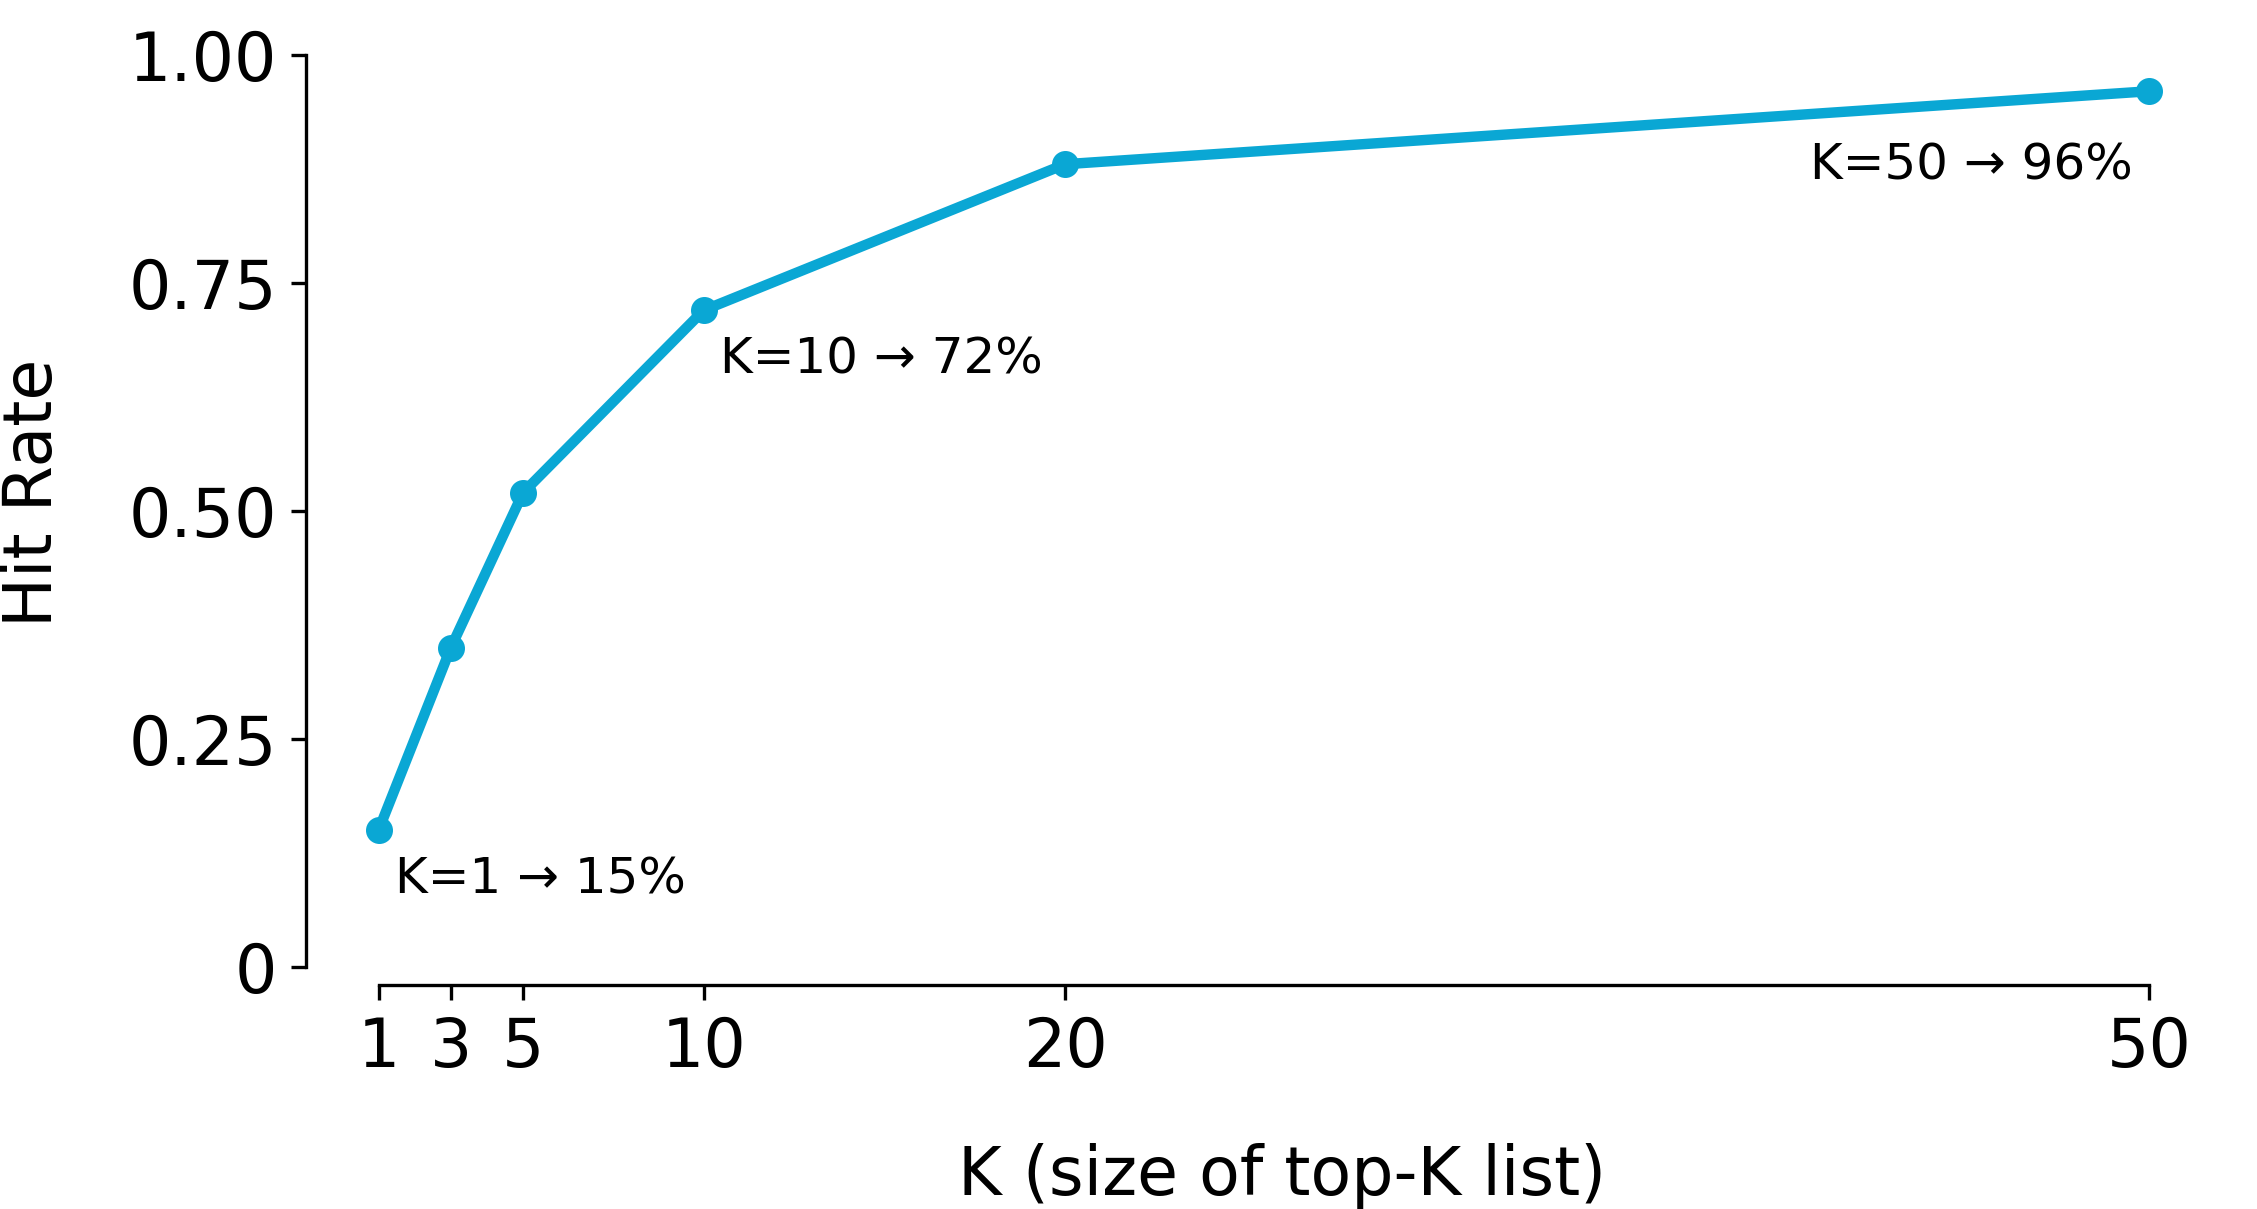
\includegraphics[width=0.6\textwidth]{figures/Hit_Rate_vs_K.png}
\end{figure*}

\textbf{Figure.} Hit Rate climbs with $K$: at $K = 1$ only $15\%$ of users see a relevant item in the first slot; at $K = 50$ that rises to $96\%$. The curve flattens as $K$ grows because the remaining failures are users with no relevant items anywhere in the top-$50$ — stretching $K$ further does not help that segment.

\orangebox{Did you know that...}
{Recommender systems papers often call Hit Rate ``Recall@$K$'' and use the two interchangeably. They are the same metric only when each user has exactly one relevant item — the typical leave-one-out evaluation setup. With multiple relevant items per user, Recall@$K$ measures the fraction retrieved, while Hit Rate stays binary. The naming clash trips up cross-paper comparisons more often than you would expect.}

\textbf{Other related metrics}

For position-aware evaluation use MRR or nDCG. For counting how many relevant items the list retrieved, use Recall@$K$. Hit Rate is the binary collapse of Recall@$K$.

% ---------- Cumulative Gain ----------
\clearpage
\thispagestyle{rankingstyle}
\section{CG}
\subsection{Cumulative Gain}

Cumulative Gain (CG) sums the relevance scores of the items in a recommendation list. With graded relevance — $3$ for ``perfect'', $1$ for ``marginal'', $0$ for ``irrelevant'' — $CG_K$ is the total relevance packed into the top-$K$. The catch is that CG ignores rank: a relevant item at position $1$ adds the same as one at position $K$.

\begin{center}
    \tikz{
        \node[inner sep=2pt, font=\Large] (a) {
            {
                $\displaystyle
                CG_p = \sum_{i=1}^{{\color{nmlred}p}} {\color{nmlcyan}rel_i}
                $
            }
        };
        \draw[overlay,-latex,nmlred, semithick] ($(a.north)+(0.8,-0.1)$) to[bend left=15] node[pos=1, right] {number of items} +(1,.5);
        \draw[overlay,-latex,nmlcyan, semithick] ($(a.south)+(1.2,0.2)$) to[bend left=15] node[pos=1, left] {relevance of item $i$} +(-1,-.5);
    }
\end{center}

CG is unbounded and order-invariant: two lists with the same items in different orders have identical CG. That makes it useful as a baseline number — ``how much total relevance did we retrieve?'' — but not as a standalone ranking metric. DCG and nDCG (next pages) fix the rank-insensitivity by discounting later positions.

\textbf{When to use CG?}

Use CG when only total retrieved relevance matters and ordering is decided downstream (a re-ranker reshuffles the list, or items are shown simultaneously). Avoid CG when position matters to the user — which covers most ranking applications. Use DCG or nDCG instead.

\coloredboxes{
    \item Simplest relevance aggregation possible: add up the scores. Trivial to compute and explain.
    \item Works with graded relevance out of the box, unlike Hit Rate or binary $Precision@K$.
}
{
    \item Order-invariant. A list with the best item at rank $1$ scores the same as one with the best item at rank $K$.
    \item Not normalized. $CG = 12$ vs $CG = 6$ across queries says nothing about which ranking was better.
    \item Falls back to a raw count of relevant items when only binary labels are available.
}

\clearpage
\thispagestyle{customstyle}

\begin{figure*}[ht!]
    \centering
    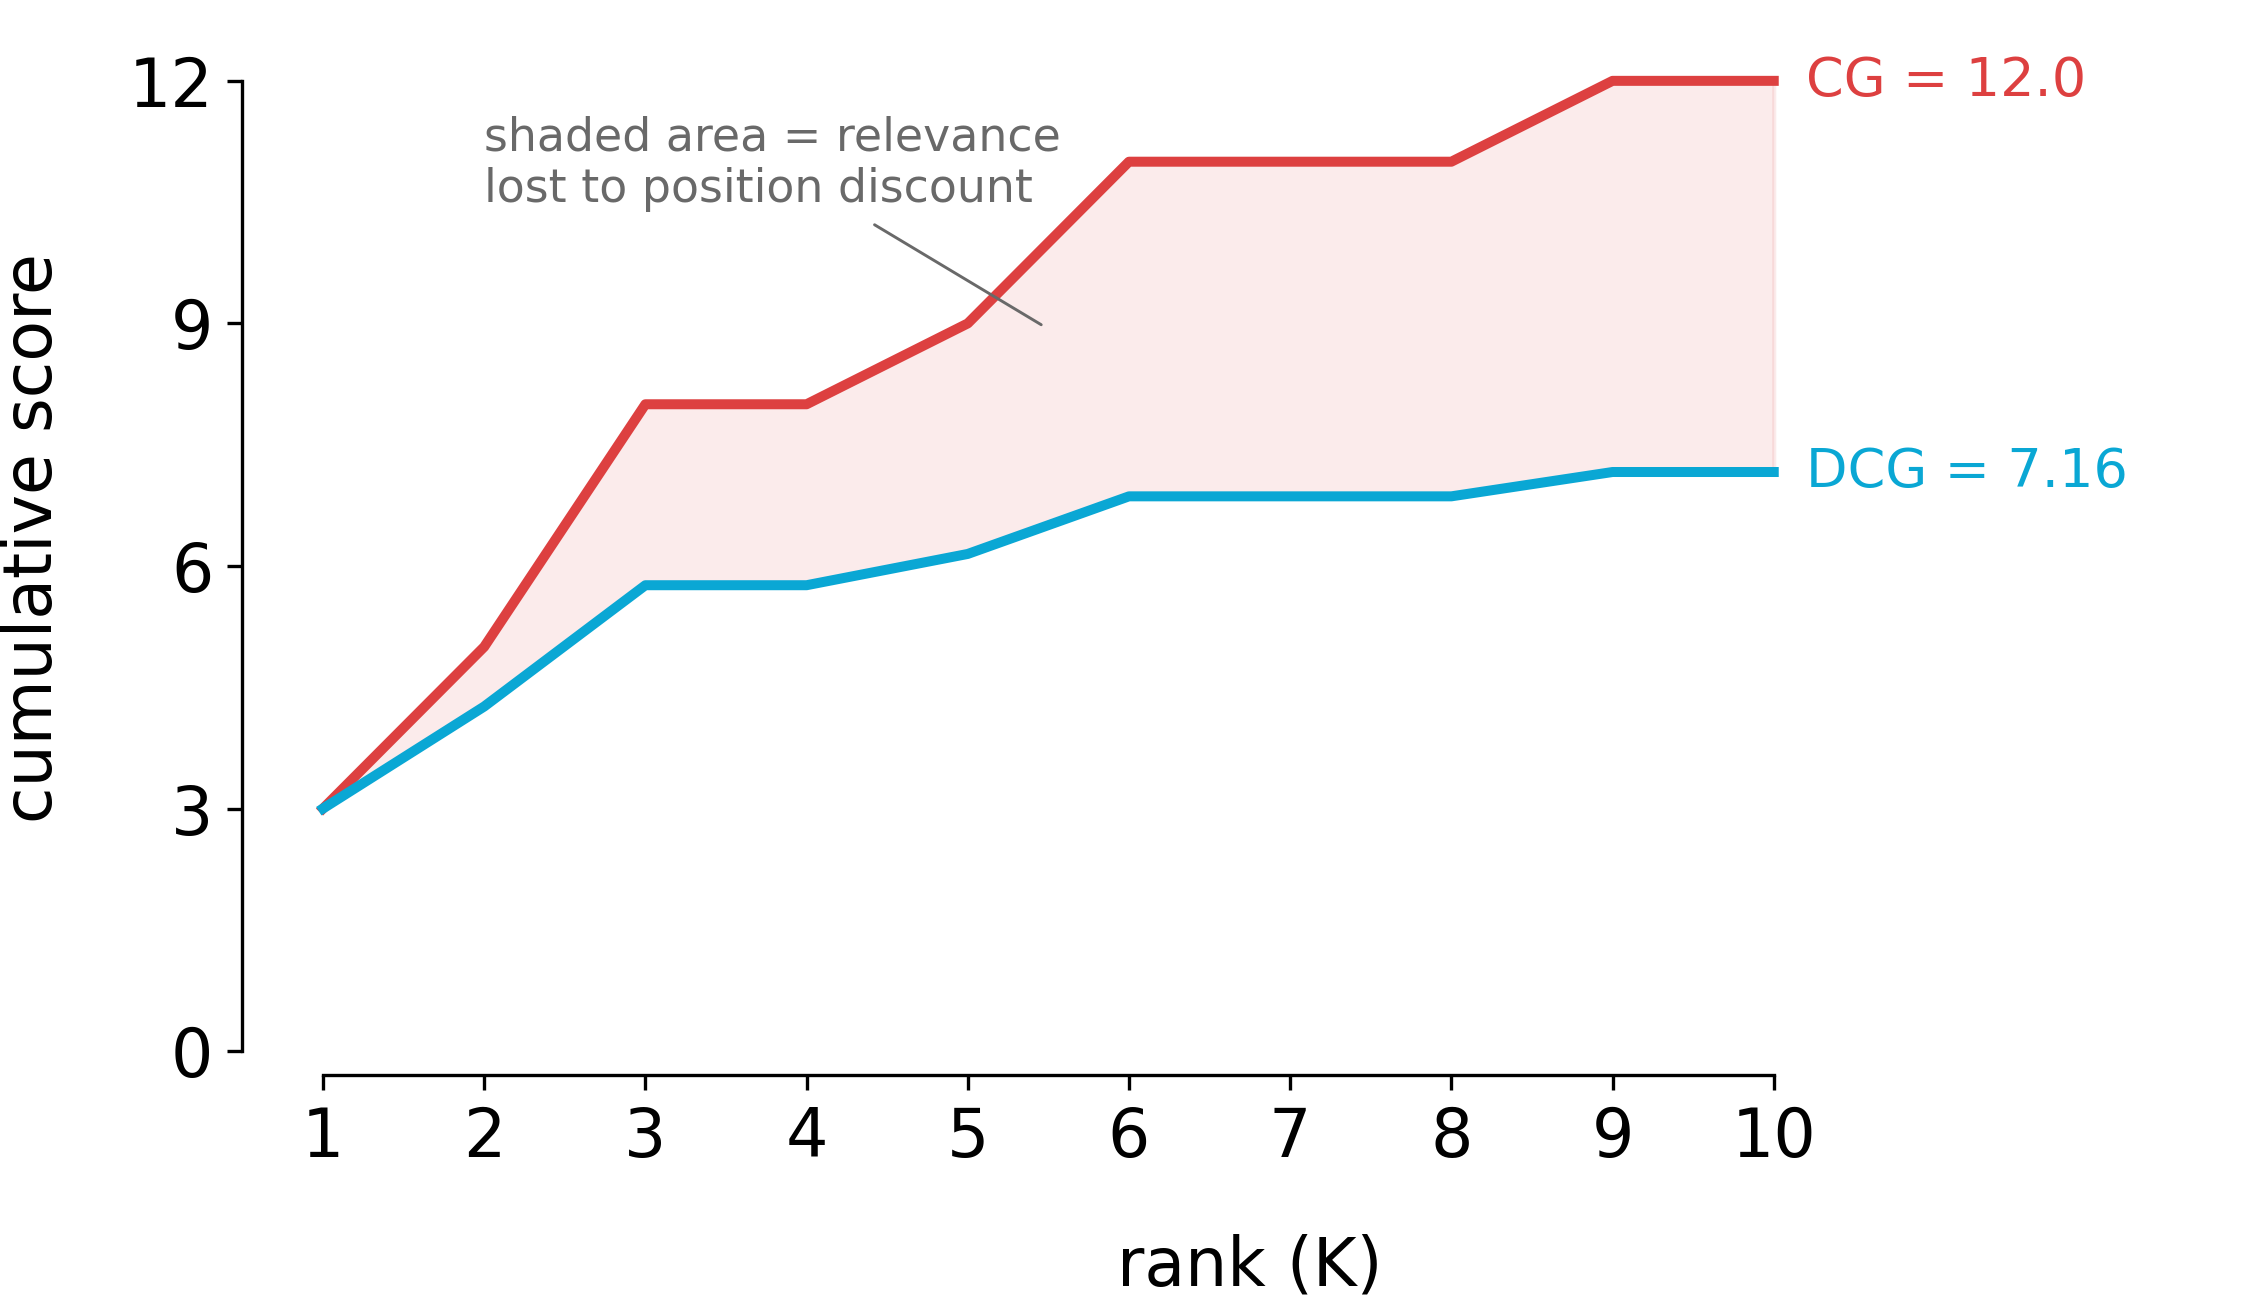
\includegraphics[width=0.6\textwidth]{figures/CG_vs_DCG.png}
\end{figure*}

\textbf{Figure.} CG (red) and DCG (blue) start at the same point — the first item contributes its full relevance to both. As $K$ grows, DCG falls behind because every position past rank $1$ takes a logarithmic discount, while CG keeps treating every position equally. The widening gap is the cost of ignoring position.

\orangebox{Did you know that...}
{The order-invariance of CG is its entire design flaw: swap any two items and the score is unchanged, which makes CG useless for ranking. The metric still gets used in retrieval-then-rerank pipelines, where the retrieval stage scores raw recall and a downstream model handles the ordering. Outside that pattern, CG on its own in a results table is a red flag.}

\textbf{Other related metrics}

DCG extends CG by discounting later positions. nDCG normalizes DCG against the ideal ranking, so scores are comparable across queries with different relevance budgets. In practice, CG is the warm-up step toward those two.

% ---------- Discounted Cumulative Gain ----------
\clearpage
\thispagestyle{rankingstyle}
\section{DCG}
\subsection{Discounted Cumulative Gain}

Discounted Cumulative Gain (DCG) improves upon CG by introducing a position-based discounting factor.
It accounts for the fact that relevant items appearing earlier in the list are more valuable than those appearing later.

\begin{center}
    \tikz{
        \node[inner sep=2pt, font=\Large] (a) {
            {
                $\displaystyle
                DCG_p = \sum_{i=1}^{{\color{nmlred}p}} \frac{{\color{nmlcyan}rel_i}}{{\color{nmlpurple}\log_2(i + 1)}}
                $
            }
        };
        \draw[overlay,-latex,nmlcyan, semithick] ($(a.north)+(1.0,-0.1)$) to[bend right=15] node[pos=1, left] {relevance of item $i$} +(-1,.5);
        \draw[overlay,-latex,nmlpurple, semithick] ($(a.south)+(1.5,0.3)$) to[bend left=15] node[pos=1, left] {position discount} +(-1,-.5);
    }
\end{center}

This logarithmic discounting ensures that higher-ranked relevant items contribute more to the score.

\textbf{When to use DCG?}

Use DCG when you want to measure both the total relevance and the order of relevant items in a ranked list. It is particularly
useful for search engines, recommendation systems, and ranking models where placing relevant items at the top is crucial.

\coloredboxes{
    \item Accounts for ranking order. Relevant items appearing earlier in the list are weighted more heavily.
    \item More realistic than CG. Since users are more likely to engage with items at the top, DCG better reflects
    real-world relevance.
}
{
    \item Not normalized — DCG values depend on the number and relevance of items, making cross-query comparison difficult.
    \item Human data labelers must provide relevance scores to compute the total accumulated relevance.
}

\clearpage
\thispagestyle{customstyle}

\begin{figure*}[ht!]
    \centering
    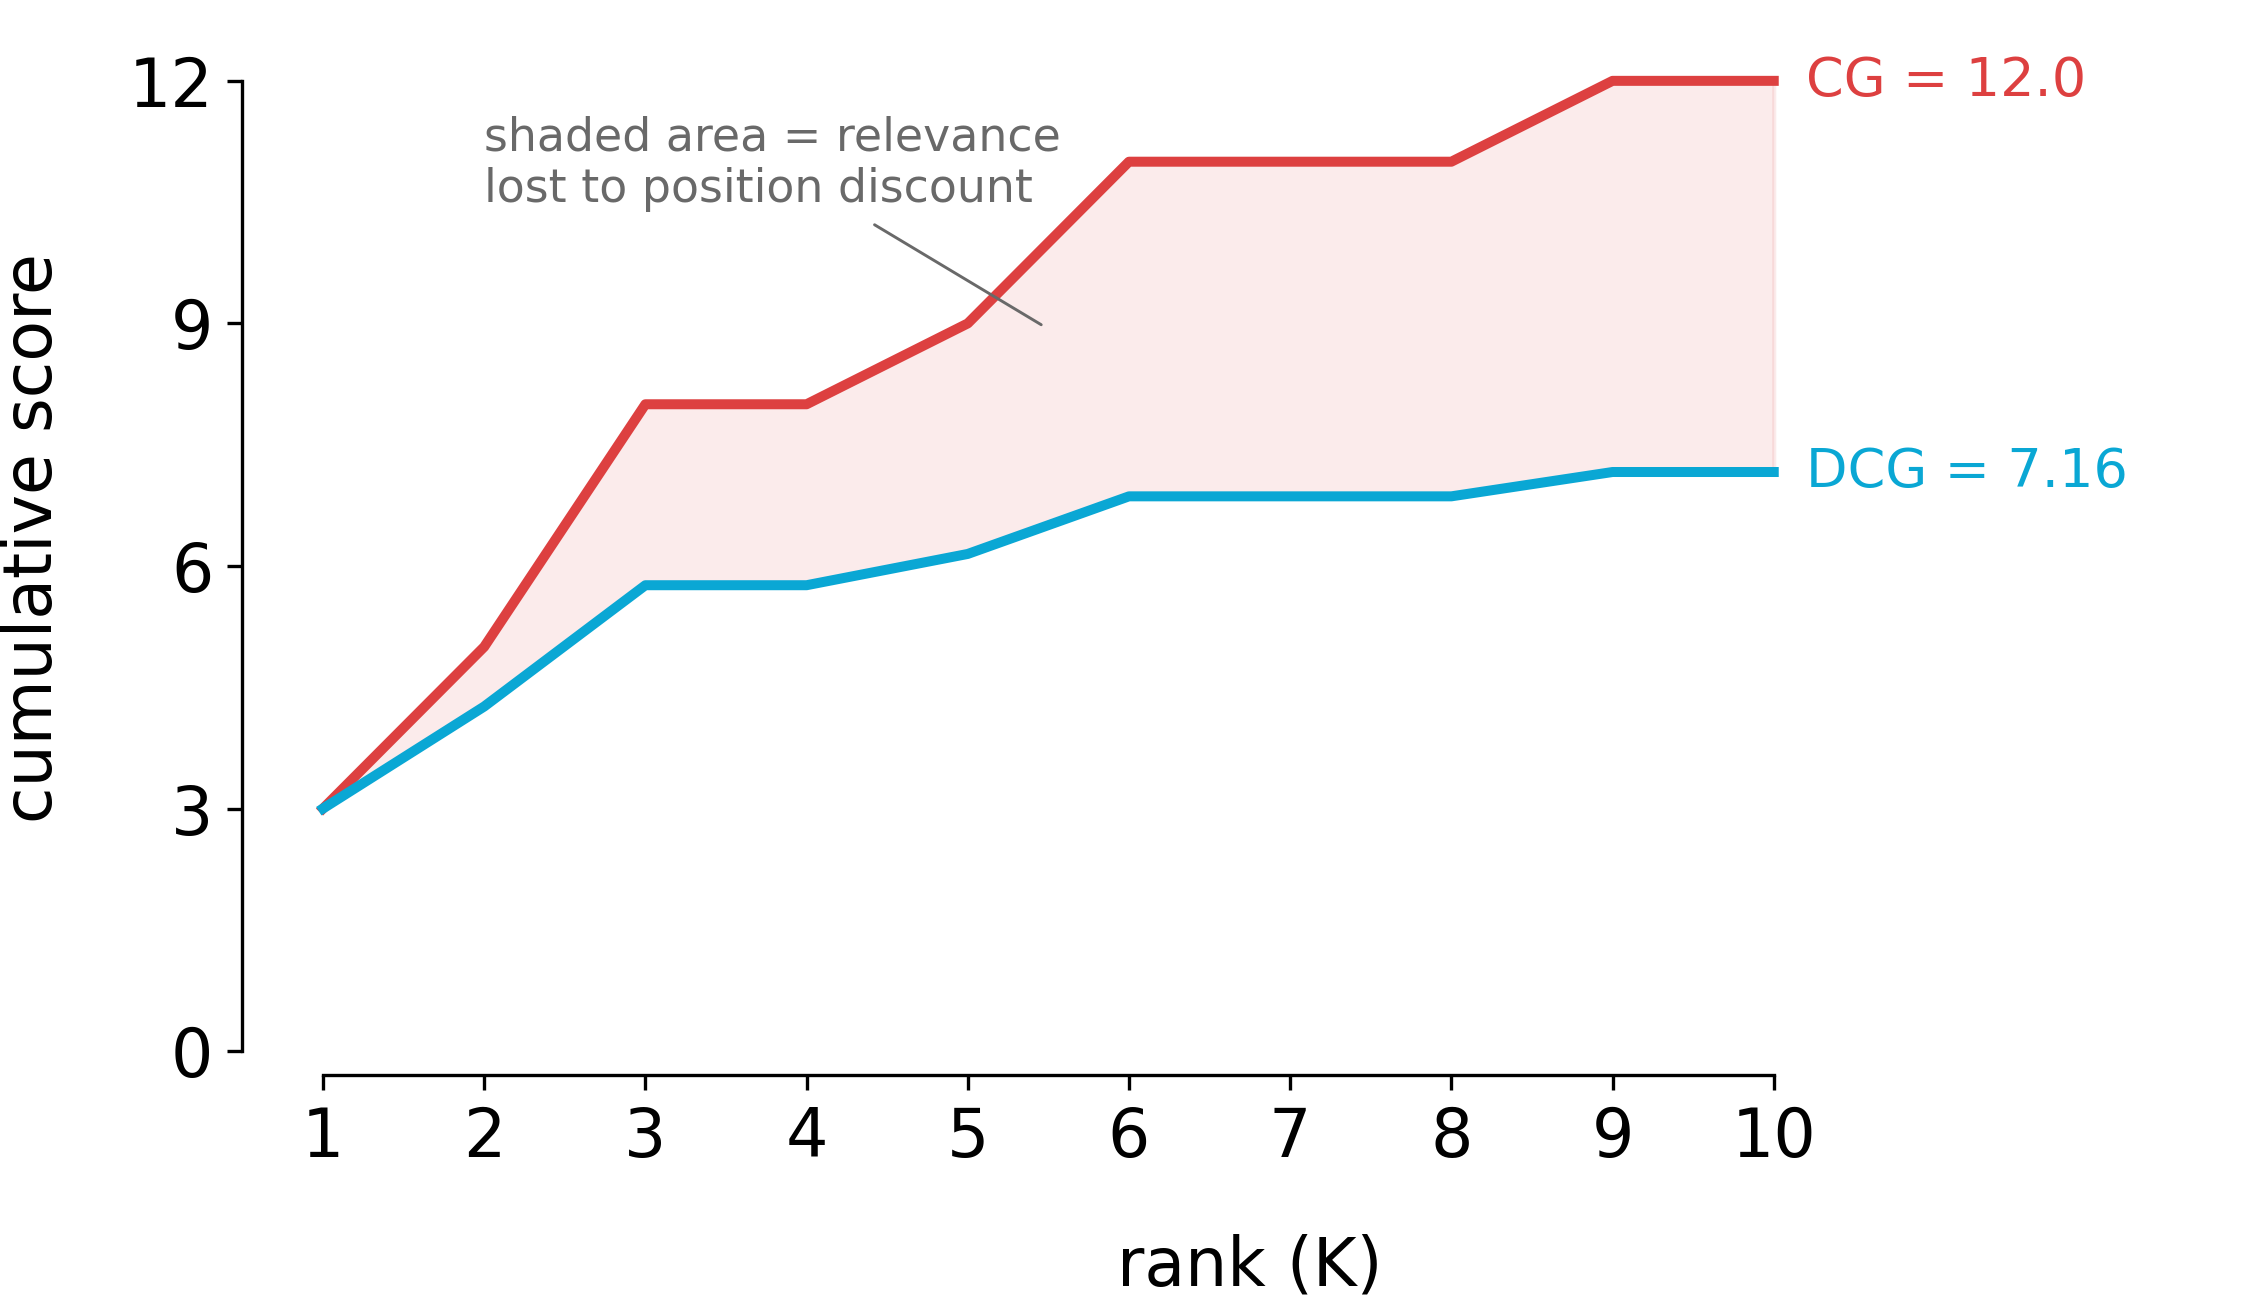
\includegraphics[width=0.6\textwidth]{figures/CG_vs_DCG.png}
\end{figure*}

\textbf{Figure.} DCG (blue) applies logarithmic discounting, giving more weight to items ranked higher. CG (red) treats all positions equally, making DCG a more realistic measure.

\orangebox{Did you know that...}
{The logarithmic discount in DCG was introduced by J\"{a}rvelin and Kek\"{a}l\"{a}inen in 2002. The choice of $\log_2$ is conventional but arbitrary — some implementations use natural log or $\log_{10}$.}

\textbf{Other related metrics}

DCG builds on CG by adding position discounting. For a normalized version that enables cross-query comparison, use nDCG.
For binary relevance, MAP may be a simpler alternative.

% ---------- Normalized Discounted Cumulative Gain ----------
\clearpage
\thispagestyle{rankingstyle}
\section{nDCG}
\subsection{Normalized Discounted Cumulative Gain}

Normalized Discounted Cumulative Gain (nDCG) extends DCG by normalizing it relative to the Ideal Discounted Cumulative Gain
(IDCG)—the best possible ranking of the same set of items. This ensures that scores are comparable across different users
and queries.

\begin{center}
    \tikz{
        \node[inner sep=2pt, font=\Large] (a) {
            {
                $\displaystyle
                nDCG_p = \frac{{\color{nmlcyan}DCG_p}}{{\color{nmlpurple}IDCG_p}}
                $
            }
        };
        \draw[overlay,-latex,nmlcyan, semithick] ($(a.north)+(0.8,-0.1)$) to[bend right=15] node[pos=1, left] {actual DCG} +(-1,.5);
        \draw[overlay,-latex,nmlpurple, semithick] ($(a.south)+(1.0,0.2)$) to[bend left=15] node[pos=1, left] {ideal DCG} +(-1,-.5);
    }
\end{center}

IDCG is the DCG computed with an optimally ranked list. nDCG values range from 0 to 1, with 1 indicating a perfect ranking.

\textbf{When to use nDCG?}

Use nDCG when you need a standardized ranking metric that allows comparison across different recommendation tasks.
It is widely used in search engines, recommender systems, and ranking models where ranking quality is essential.

\coloredboxes{
    \item Scale-independent. Since it is normalized, NDCG values are comparable across different datasets and users.
    \item Captures both relevance and ranking order. It rewards placing highly relevant items early in the list while
    penalizing poorly ranked relevant items.
}
{
    \item Human data labelers must provide relevance scores to compute the total accumulated relevance.
    \item Not ideal for binary relevance. nDCG is designed for graded relevance; for binary relevance, MAP may be more appropriate.
}

\clearpage
\thispagestyle{customstyle}

\begin{figure*}[ht!]
    \centering
    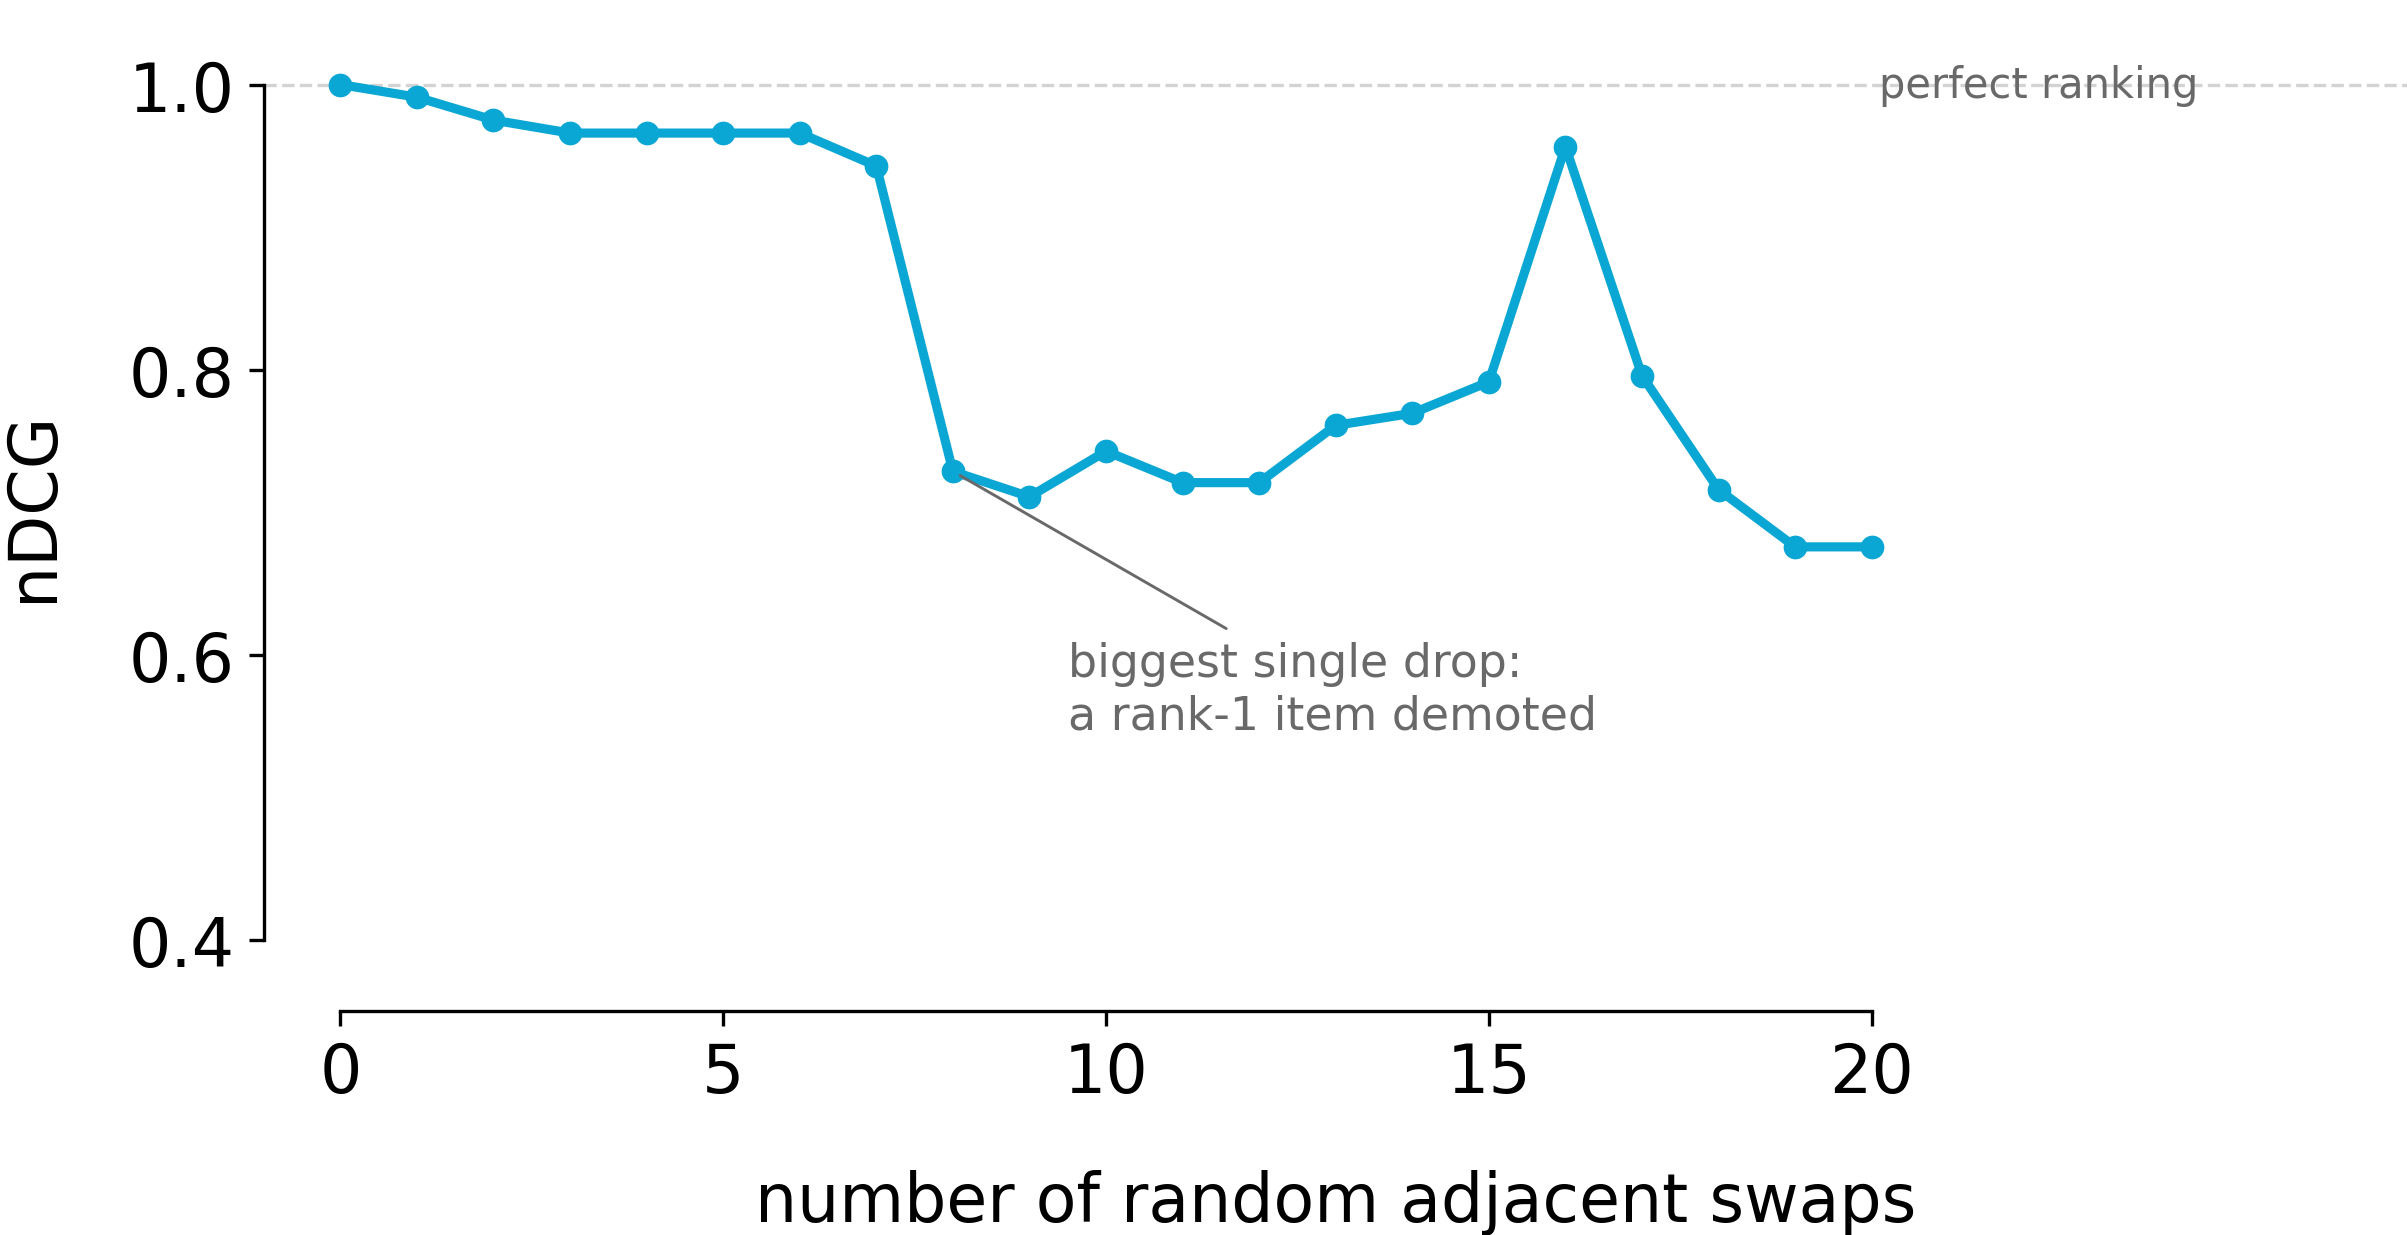
\includegraphics[width=0.6\textwidth]{figures/nDCG_degradation.png}
\end{figure*}

\textbf{Figure.} nDCG decreases as we progressively degrade the ranking by random swaps. A perfect ranking scores 1.0; each swap moves relevant items away from their ideal positions.

\orangebox{Did you know that...}
{nDCG is the standard offline evaluation metric at most major tech companies for search and recommendation systems. It is also the primary metric
used in the annual TREC Web Track and in Kaggle recommendation competitions.}

\textbf{Other related metrics}

nDCG is the normalized version of DCG. For binary relevance scenarios, consider MAP. For evaluating only the first relevant result, use MRR.

% great resource: https://aman.ai/recsys/metrics/#normalized-discounted-cumulative-gain-ndcg-1


% ---------- Fraction of Concordant Pairs ----------
\clearpage
\thispagestyle{rankingstyle}
\section{FCP}
\subsection{Fraction of Concordant Pairs}

Fraction of Concordant Pairs (FCP) is a ranking metric used in recommender systems to evaluate how well a model ranks
preferred items higher than less preferred ones. It measures the proportion of correctly ordered item pairs among all
comparable pairs in a recommendation list. Given a user’s interactions, FCP checks whether the model ranks a more relevant
item above a less relevant one.

\begin{center}
    \tikz{
        \node[inner sep=2pt, font=\Large] (a) {
            {
                $\displaystyle
                FCP = \frac{|{\color{nmlcyan}\text{concordant pairs}}|}{|{\color{nmlpurple}\text{comparable pairs}}|}
                $
            }
        };
        \draw[overlay,-latex,nmlcyan, semithick] ($(a.north)+(0.5,-0.1)$) to[bend right=15] node[pos=1, left] {correctly ordered pairs} +(-1,.5);
        \draw[overlay,-latex,nmlpurple, semithick] ($(a.south)+(1.0,0.3)$) to[bend left=15] node[pos=1, left] {total comparable pairs} +(-1,-.5);
    }
\end{center}

A concordant pair is one where the model correctly ranks a preferred item above a less preferred one. FCP values range from
0 to 1, with 1 indicating a perfect ranking and 0 meaning the model fails to rank preferred items higher.

\textbf{When to use FCP?}

Use FCP when evaluating recommender systems that generate personalized rankings, especially in cases where relative
ranking quality is more important than absolute scores. It is particularly useful in implicit feedback scenarios,
such as e-commerce or media streaming, where explicit relevance scores are unavailable, and user preferences must be
inferred from interactions.

\coloredboxes{
    \item It directly measures how accurately the system's rankings align with user preferences.
}
{
    \item It only evaluates pairs of items where user preferences can be inferred, potentially reducing
    the number of evaluated pairs.
    \item Calculating FCP can be resource-intensive for large datasets, as the number of item pairs grows
    quadratically with dataset size.
}

\clearpage
\thispagestyle{customstyle}

\begin{figure*}[ht!]
    \centering
    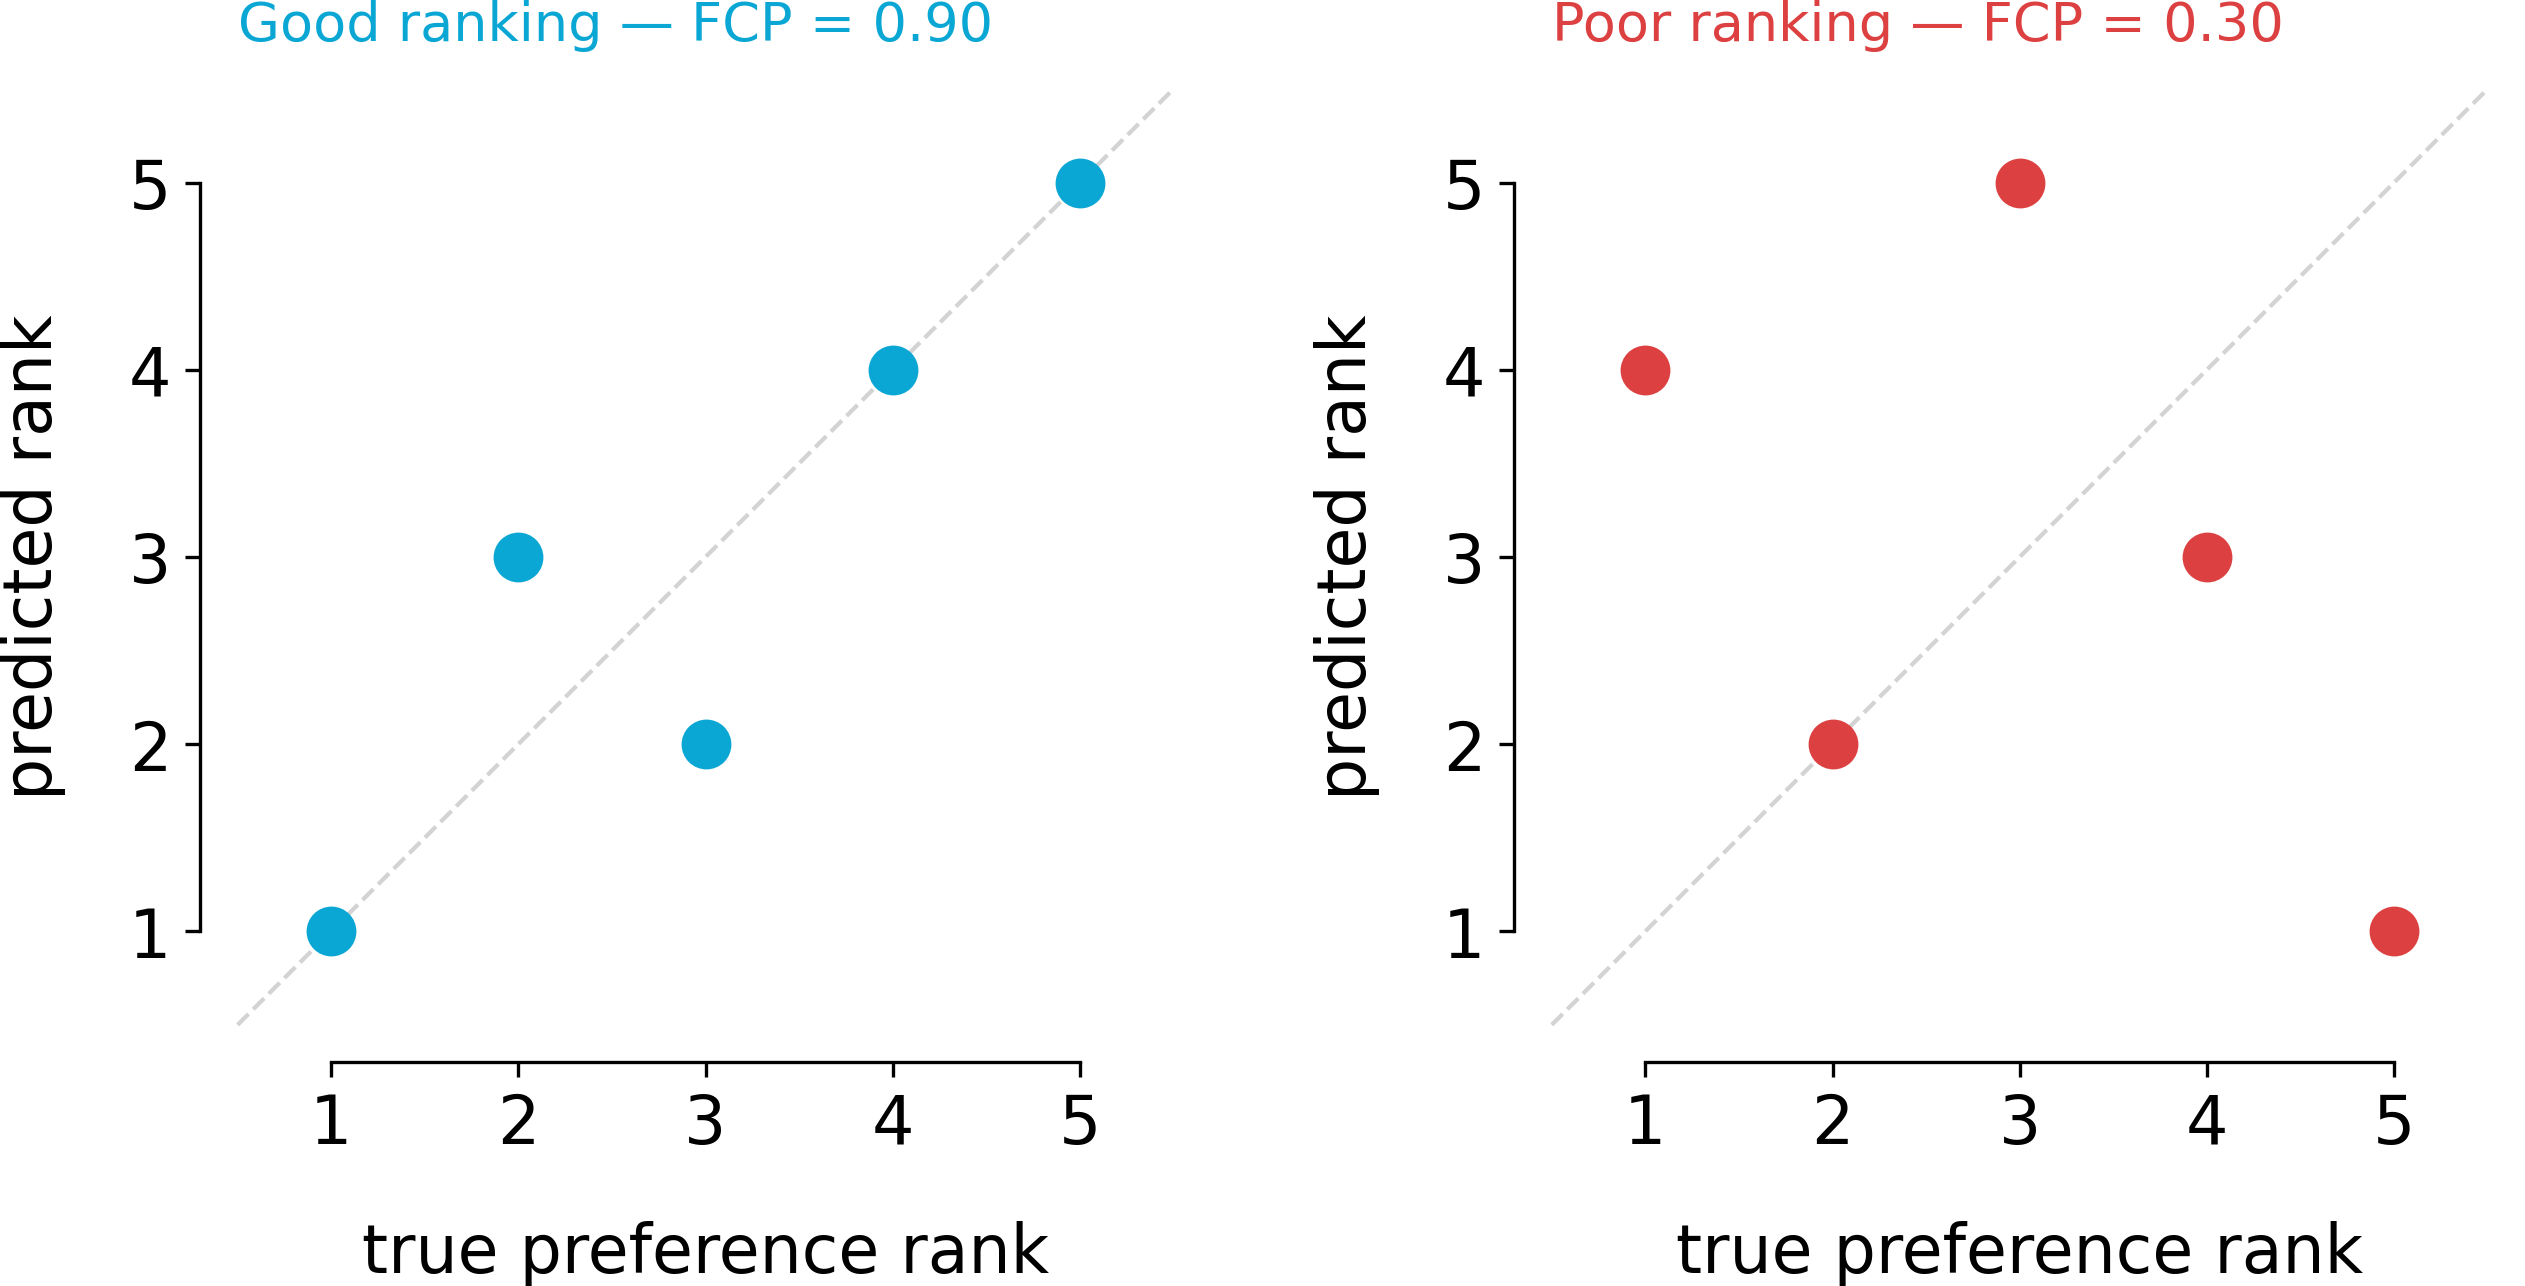
\includegraphics[width=\textwidth]{figures/FCP_comparison.png}
\end{figure*}

\textbf{Figure.} A good ranking (left, FCP=0.90) shows predicted ranks closely matching true preferences. A poor ranking (right, FCP=0.20) shows little agreement.

\orangebox{Did you know that...}
{FCP is closely related to Kendall's tau rank correlation coefficient. Both measure pairwise agreement in rankings, but FCP is expressed as a proportion
while Kendall's tau is normalized to [-1, 1].}

\textbf{Other related metrics}

FCP is a pairwise ranking metric similar to Kendall's tau and Spearman's rank correlation.
For position-weighted evaluation, use nDCG or MAP instead.

% great references: https://aman.ai/recsys/metrics/#fraction-of-concordant-pairs-fcp
% https://www.ijcai.org/Proceedings/13/Papers/449.pdf

% ---------- Diversity ----------
\clearpage
\thispagestyle{rankingstyle}
\section{Diversity}
\subsection{Diversity}

Diversity is a ranking metric used in recommender systems to measure how varied the recommended items are within a given list.
A diverse recommendation set ensures that users are exposed to different categories, genres, or types of content, rather than
receiving highly similar items. This helps prevent redundancy and enhances user discovery. Diversity is often calculated using
pairwise dissimilarity between recommended items.

\begin{center}
    \tikz{
        \node[inner sep=2pt, font=\Large] (a) {
            {
                $\displaystyle
                Diversity = \frac{1}{{\color{nmlred}|L|(|L|-1)}} \sum_{i \in L} \sum_{j \in L, j \neq i} {\color{nmlcyan}d(i, j)}
                $
            }
        };
        \draw[overlay,-latex,nmlred, semithick] ($(a.south)+(-1.5,0.2)$) to[bend left=15] node[pos=1, left] {list size} +(-1,-.5);
        \draw[overlay,-latex,nmlcyan, semithick] ($(a.north)+(3.0,-0.1)$) to[bend left=15] node[pos=1, right] {pairwise dissimilarity} +(1,.5);
    }
\end{center}

A higher Diversity score indicates that the recommended items are more distinct from one another, whereas a lower score
suggests redundancy.

\textbf{When to use Diversity?}

Diversity is particularly important when you want to improve user engagement by introducing varied recommendations. Or when
you want to avoid excessive similarity in recommendations.

\coloredboxes{
    \item Encourages exploration. Users are exposed to a broader range of content, which can increase
    engagement and retention.
    \item Supports long-tail recommendations. Helps surface less popular items that may still be relevant,
    avoiding over-recommendation of mainstream content.
}
{
    \item Potential trade-off with relevance. Increasing diversity may sometimes lead to less relevant recommendations
    for the user.
    \item Hard to define optimal diversity. Too much diversity can lead to recommendations that feel random or disconnected.
}

\clearpage
\thispagestyle{customstyle}

\begin{figure*}[ht!]
    \centering
    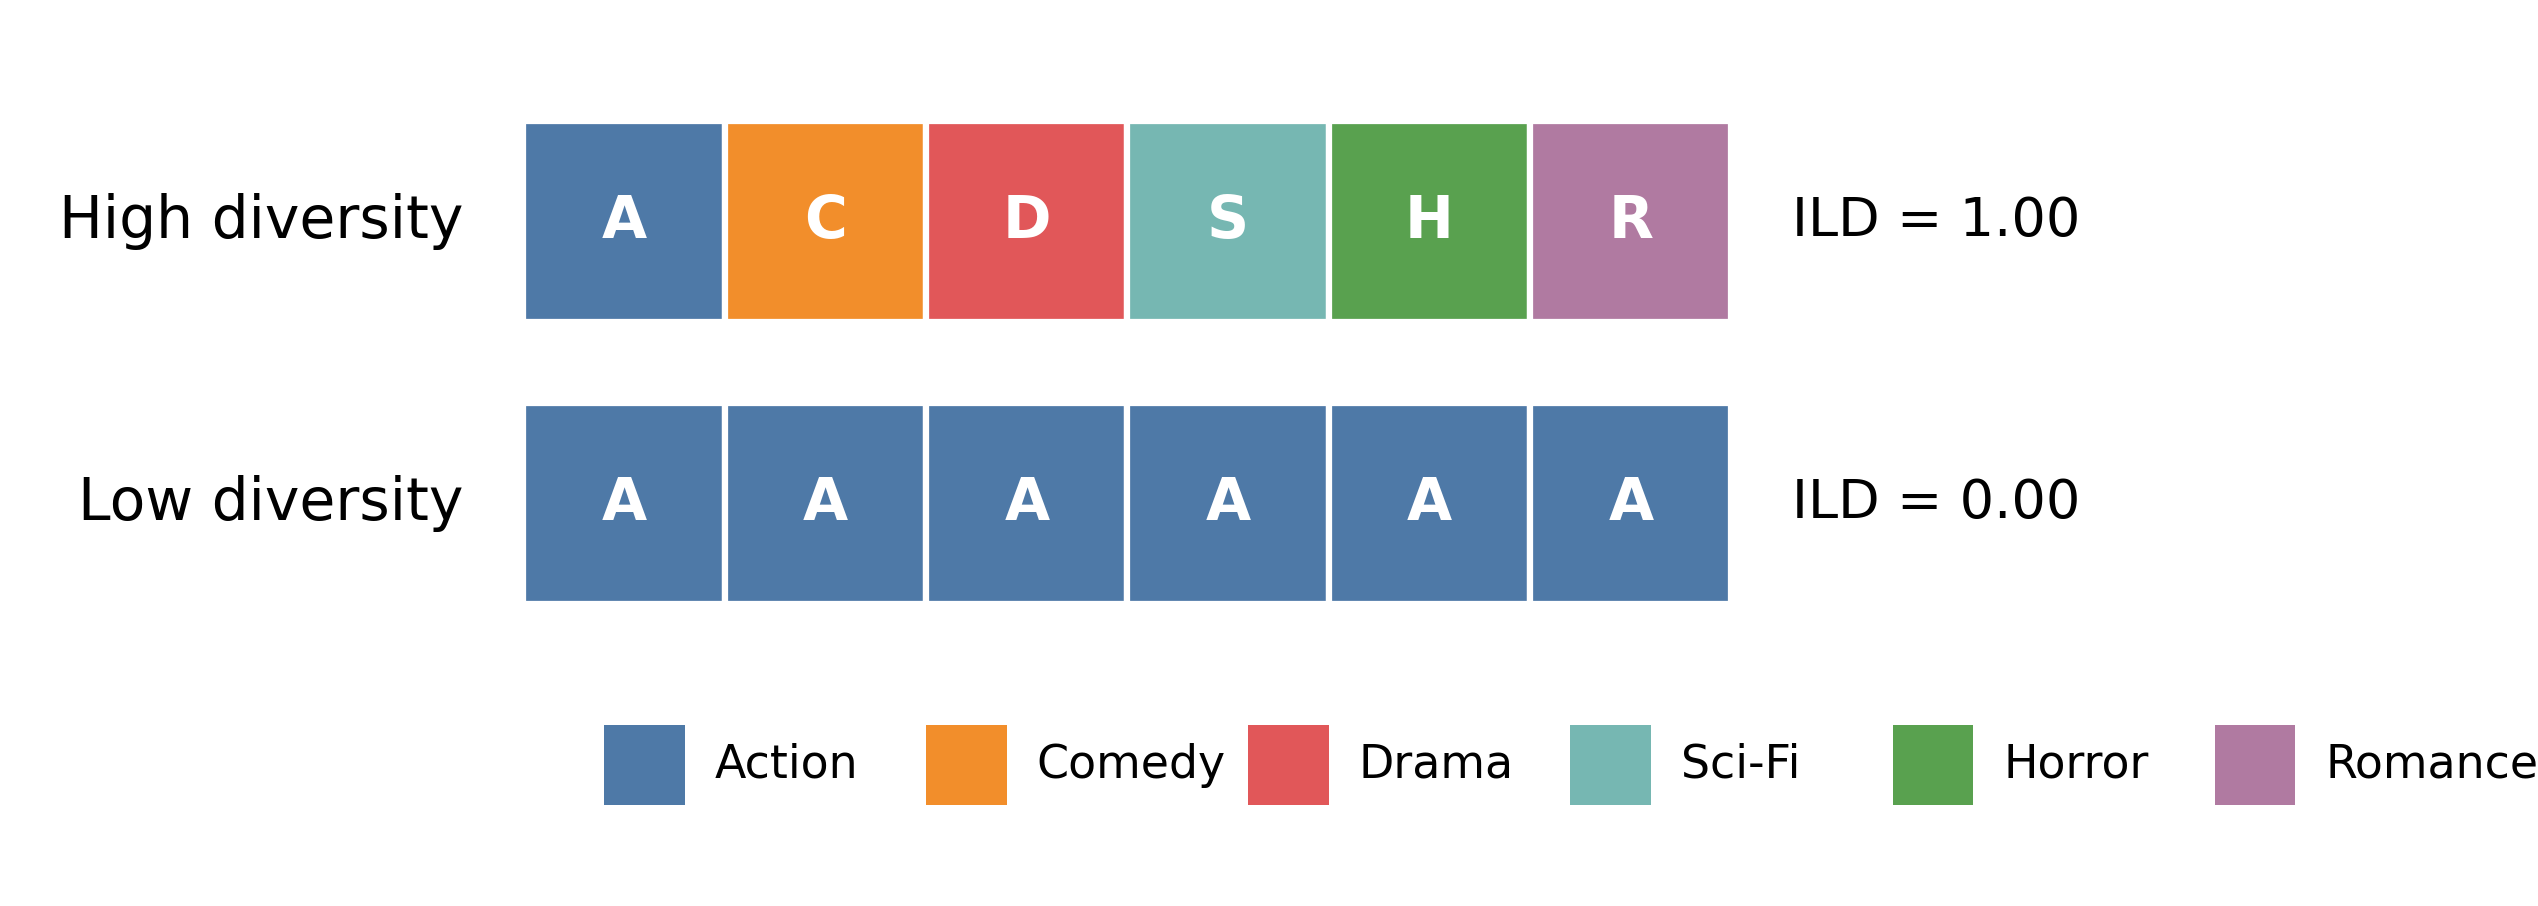
\includegraphics[width=\textwidth]{figures/Diversity_comparison.png}
\end{figure*}

\textbf{Figure.} High diversity (left) spreads recommendations across multiple genres. Low diversity (right) concentrates all recommendations in a single genre.

\orangebox{Did you know that...}
{Intra-List Diversity (ILD) is the most common formulation of diversity in recommender systems. The choice of dissimilarity function $d(i,j)$
is crucial — common options include 1 minus cosine similarity of item feature vectors, or genre/category distance.}

\textbf{Other related metrics}

Diversity measures how different items are from each other, while Novelty measures how new items are to the user.
Serendipity combines both relevance and unexpectedness. Coverage measures catalog utilization.

% ---------- Novelty ----------
\clearpage
\thispagestyle{rankingstyle}
\section{Novelty}
\subsection{Novelty}

Novelty is a ranking metric in recommender systems that measures how unfamiliar or unexpected the recommended items are to
the user. A high Novelty score indicates that the system is suggesting items that the user has not encountered before,
rather than repeating well-known or frequently recommended content. One way to measure Novelty is the following.

\begin{center}
    \[
        Novelty(i) = 1 - \frac{count(\text{users who got recommended} \: i)}{count(\text{users who have not interacted with} \: i)}
    \]
\end{center}

In the literature we can find other ways to compute Novelty such as: $Novelty(i) = -log_2 \left( \frac{count(\text{users who got recommended } \: i)}{count(\text{users who have not interacted with} \: i)} \right)$
or $Novelty = \frac{1}{|S|} \sum_{i \in S} -log P(i)$ where $P(i)$ represents the popularity of item \( i \)
A higher Novelty score means the recommendations contain less mainstream content, encouraging discovery of new items rather
than reinforcing existing preferences.

\textbf{When to use Novelty?}

Novelty is especially useful in scenarios where exploration and discovery are important. Such as content, e-commerce and
retail platforms where recommending new or niche products rather than just trending or best-selling ones can make a difference.

\coloredboxes{
    \item Encourages exploration. Users are exposed to a broader range of content, which can increase
    engagement and retention.
    \item Supports discovery of niche content. Helps mitigate the popularity bias by promoting lesser-known items.
}
{
    \item Potential Trade-off with relevance. High novelty items might be less relevant if the user has no prior
    interest in them.
    \item Potentially overwhelming for users. If novelty is too high, recommendations may feel random or disconnected.
}


\clearpage
\thispagestyle{customstyle}

\begin{figure*}[ht!]
    \centering
    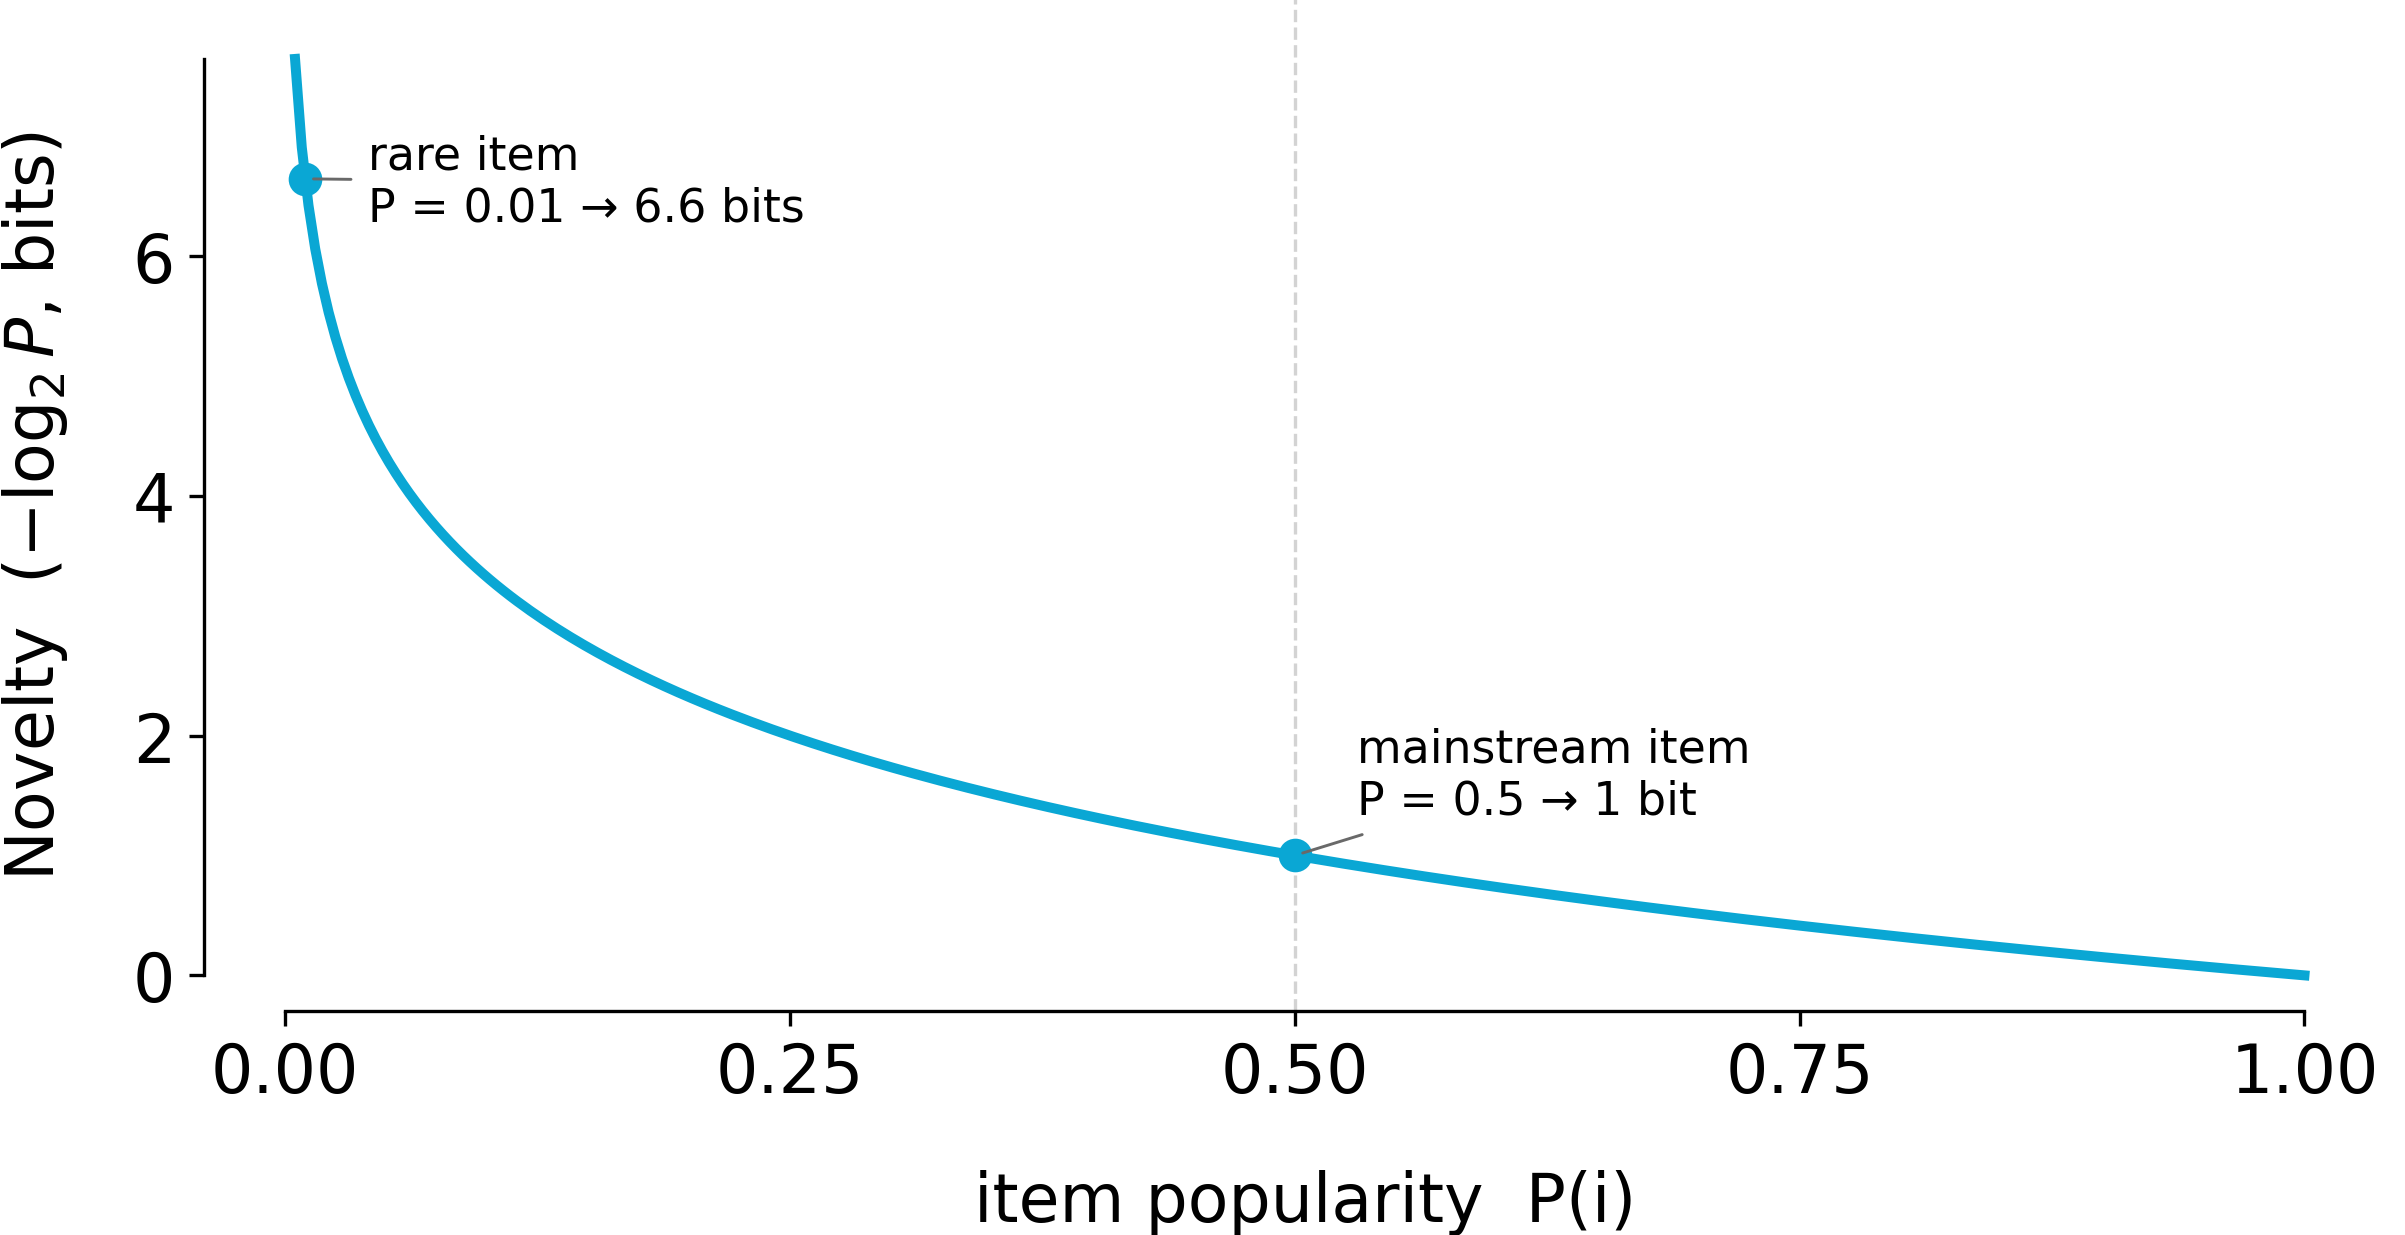
\includegraphics[width=0.6\textwidth]{figures/Novelty_curve.png}
\end{figure*}

\textbf{Figure.} Novelty as a function of item popularity. Rare items (low popularity) have high novelty, while mainstream items have near-zero novelty.

\orangebox{Did you know that...}
{The self-information formulation $Novelty(i) = -\log_2 P(i)$ is borrowed from information theory. A popular item with $P(i) = 0.5$ has novelty of 1 bit,
while a rare item with $P(i) = 0.01$ has novelty of 6.6 bits.}

\textbf{Novelty vs Diversity}

Novelty focuses on how new or unexpected the recommendations are for the user whereas diversity focuses on how different the
recommended items are from each other. Both metrics contribute to exploration but in different ways — novelty ensures
fresh discoveries, while diversity prevents redundancy.

\textbf{Other related metrics}

Novelty is complementary to Diversity and Serendipity. For measuring catalog utilization, see Coverage.
For accuracy-focused ranking evaluation, use nDCG or MAP.

% ---------- Serendipity ----------
\clearpage
\thispagestyle{rankingstyle}
\section{Serendipity}
\subsection{Serendipity}

Serendipity is a ranking and recommendation system metric that measures the extent to which a recommendation is both
relevant and surprising to a user. Unlike conventional accuracy-based metrics, which focus on predicting user preferences
based on past behavior, serendipity evaluates how well a system introduces users to novel and unexpected items they would
not have easily discovered themselves.

\begin{center}
    \tikz{
        \node[inner sep=2pt, font=\Large] (a) {
            {
                $\displaystyle
                Serendipity = \frac{1}{{\color{nmlred}N}} \sum_{i=1}^{N} {\color{nmlcyan}rel(i)} \cdot {\color{nmlpurple}unexp(i)}
                $
            }
        };
        \draw[overlay,-latex,nmlred, semithick] ($(a.south)+(-1.0,0.2)$) to[bend left=15] node[pos=1, left] {number of items} +(-1,-.5);
        \draw[overlay,-latex,nmlcyan, semithick] ($(a.north)+(1.5,-0.1)$) to[bend right=15] node[pos=1, left] {relevance} +(-1,.5);
        \draw[overlay,-latex,nmlpurple, semithick] ($(a.north)+(3.0,-0.1)$) to[bend left=15] node[pos=1, right] {unexpectedness} +(1,.5);
    }
\end{center}

A high serendipity score means the system provides relevant and pleasantly surprising recommendations, while a low score
indicates predictable suggestions.

\textbf{When to use Serendipity?}

Use serendipity when designing recommender systems that aim to provide diverse and engaging recommendations beyond what
users already know. It is particularly useful in domains like music streaming and movie recommendations, where user
satisfaction improves when they encounter unexpected but enjoyable suggestions.

\coloredboxes{
    \item Encourages discovery: Helps users explore new items they wouldn't typically encounter.
    \item Improves long-term engagement. By avoiding repetitive recommendations, it keeps users engaged with the platform.
}
{
    \item Hard to quantify "unexpectedness".
    \item Trade-off with accuracy. Maximizing serendipity may reduce traditional accuracy metrics.
}

\clearpage
\thispagestyle{customstyle}

\begin{figure*}[ht!]
    \centering
    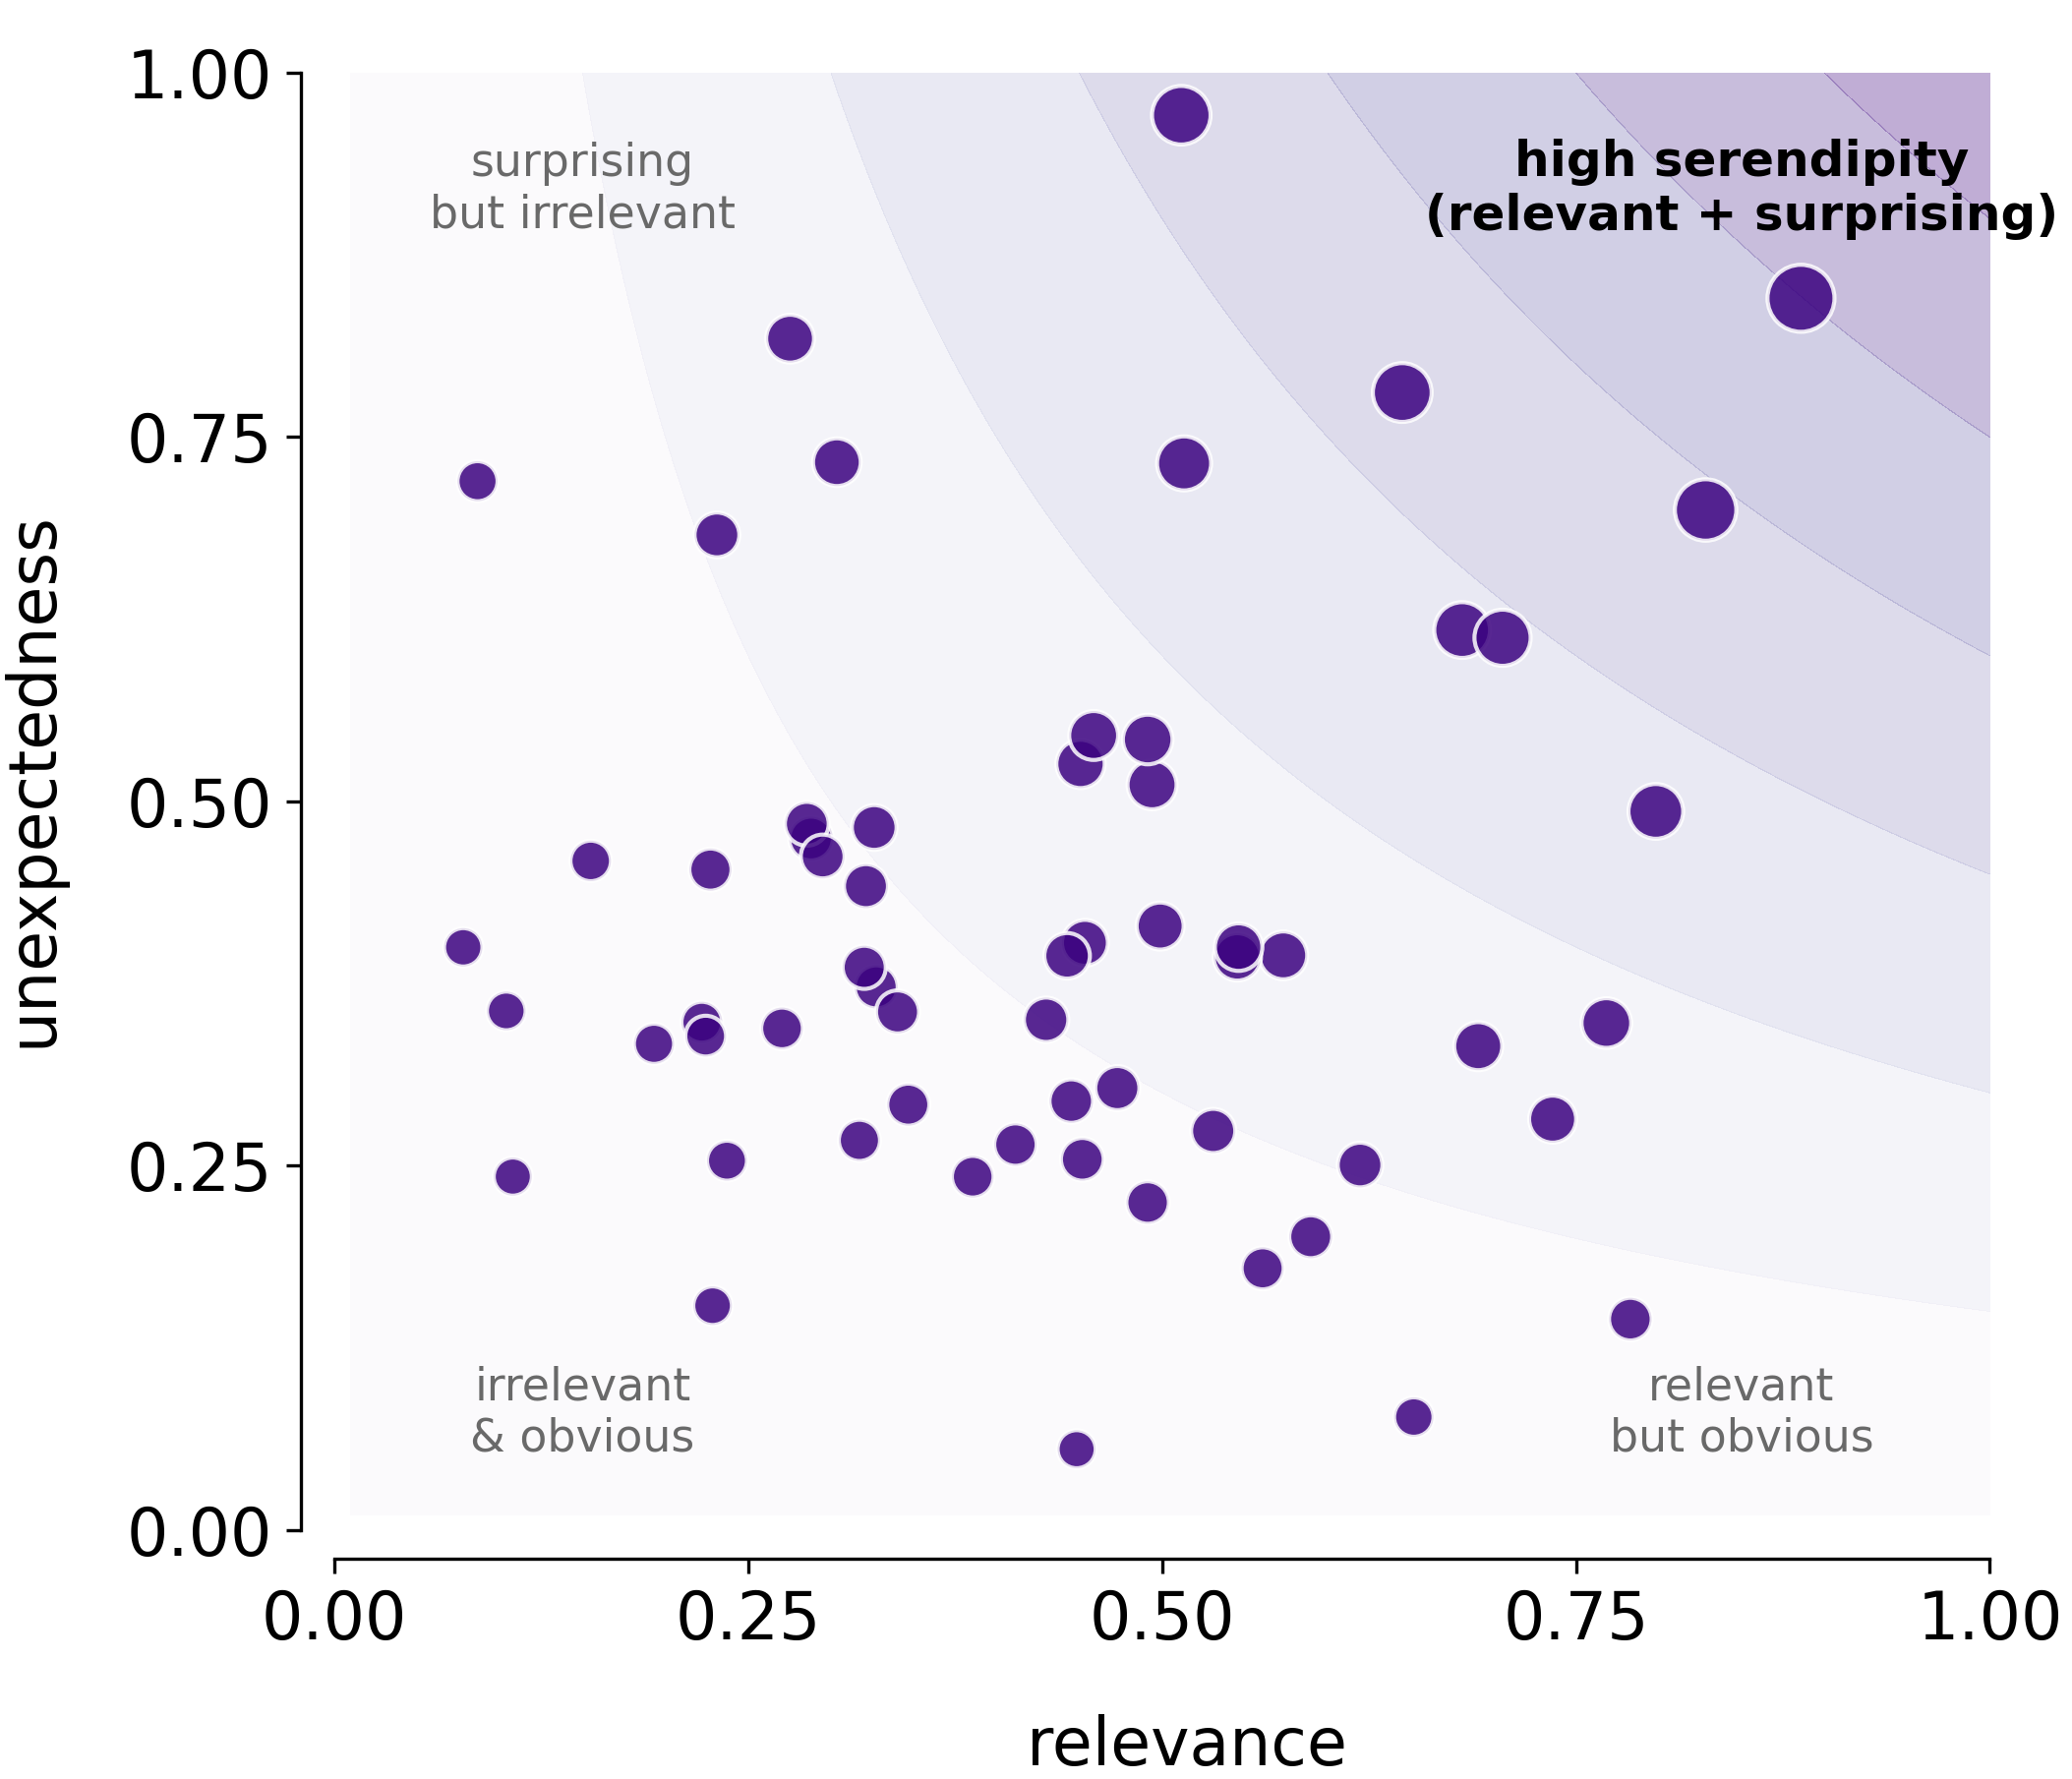
\includegraphics[width=0.6\textwidth]{figures/Serendipity_scatter.png}
\end{figure*}

\textbf{Figure.} Each point is a recommended item. Serendipity is highest (dark) when items are both relevant AND unexpected. The upper-right quadrant represents the ideal serendipitous recommendations.

\orangebox{Did you know that...}
{The term serendipity comes from the 1754 fairy tale "The Three Princes of Serendip." In recommender systems, it captures the idea of
a "happy accident" — finding something valuable that you weren't looking for.}

\textbf{Other related metrics}

Serendipity combines relevance (like Precision) with unexpectedness (like Novelty). For measuring variety without
considering relevance, use Diversity. For catalog breadth, see Coverage.

% ---------- Coverage ----------
\clearpage
\thispagestyle{rankingstyle}
\section{Coverage}
\subsection{Coverage}

Coverage measures how well a recommender system utilizes the full range of available items. It reflects the proportion of
the item catalog that is being recommended to users, ensuring that recommendations are not overly concentrated on a small
subset of popular items. 

\begin{center}
    \tikz{
        \node[inner sep=2pt, font=\Large] (a) {
            {
                $\displaystyle
                Coverage = \frac{|{\color{nmlcyan}\text{recommended items}}|}{|{\color{nmlpurple}\text{total catalog}}|}
                $
            }
        };
        \draw[overlay,-latex,nmlcyan, semithick] ($(a.north)+(0.5,-0.1)$) to[bend right=15] node[pos=1, left] {unique recommended} +(-1,.5);
        \draw[overlay,-latex,nmlpurple, semithick] ($(a.south)+(1.0,0.3)$) to[bend left=15] node[pos=1, left] {total catalog items} +(-1,-.5);
    }
\end{center}

Higher coverage indicates a broader, more diverse recommendation set, while lower coverage suggests a system that primarily
focuses on frequently chosen or trending items.

\textbf{When to use Coverage?}

Use coverage when evaluating how well a recommender system distributes recommendations across the entire catalog. 
It is particularly useful for platforms where content discovery is a priority. If a system recommends only a small fraction
of the available items, users may miss out on relevant but less popular choices.

\coloredboxes{
    \item Reduces popularity bias. Encourages recommendations beyond just the most popular or frequently interacted items.
    \item Enhances user discovery. Helps users explore content they may not have found otherwise.
}
{
    \item Can reduce recommendation accuracy. Expanding recommendations too broadly may lead to less relevant suggestions.
}

\clearpage
\thispagestyle{customstyle}

\begin{figure*}[ht!]
    \centering
    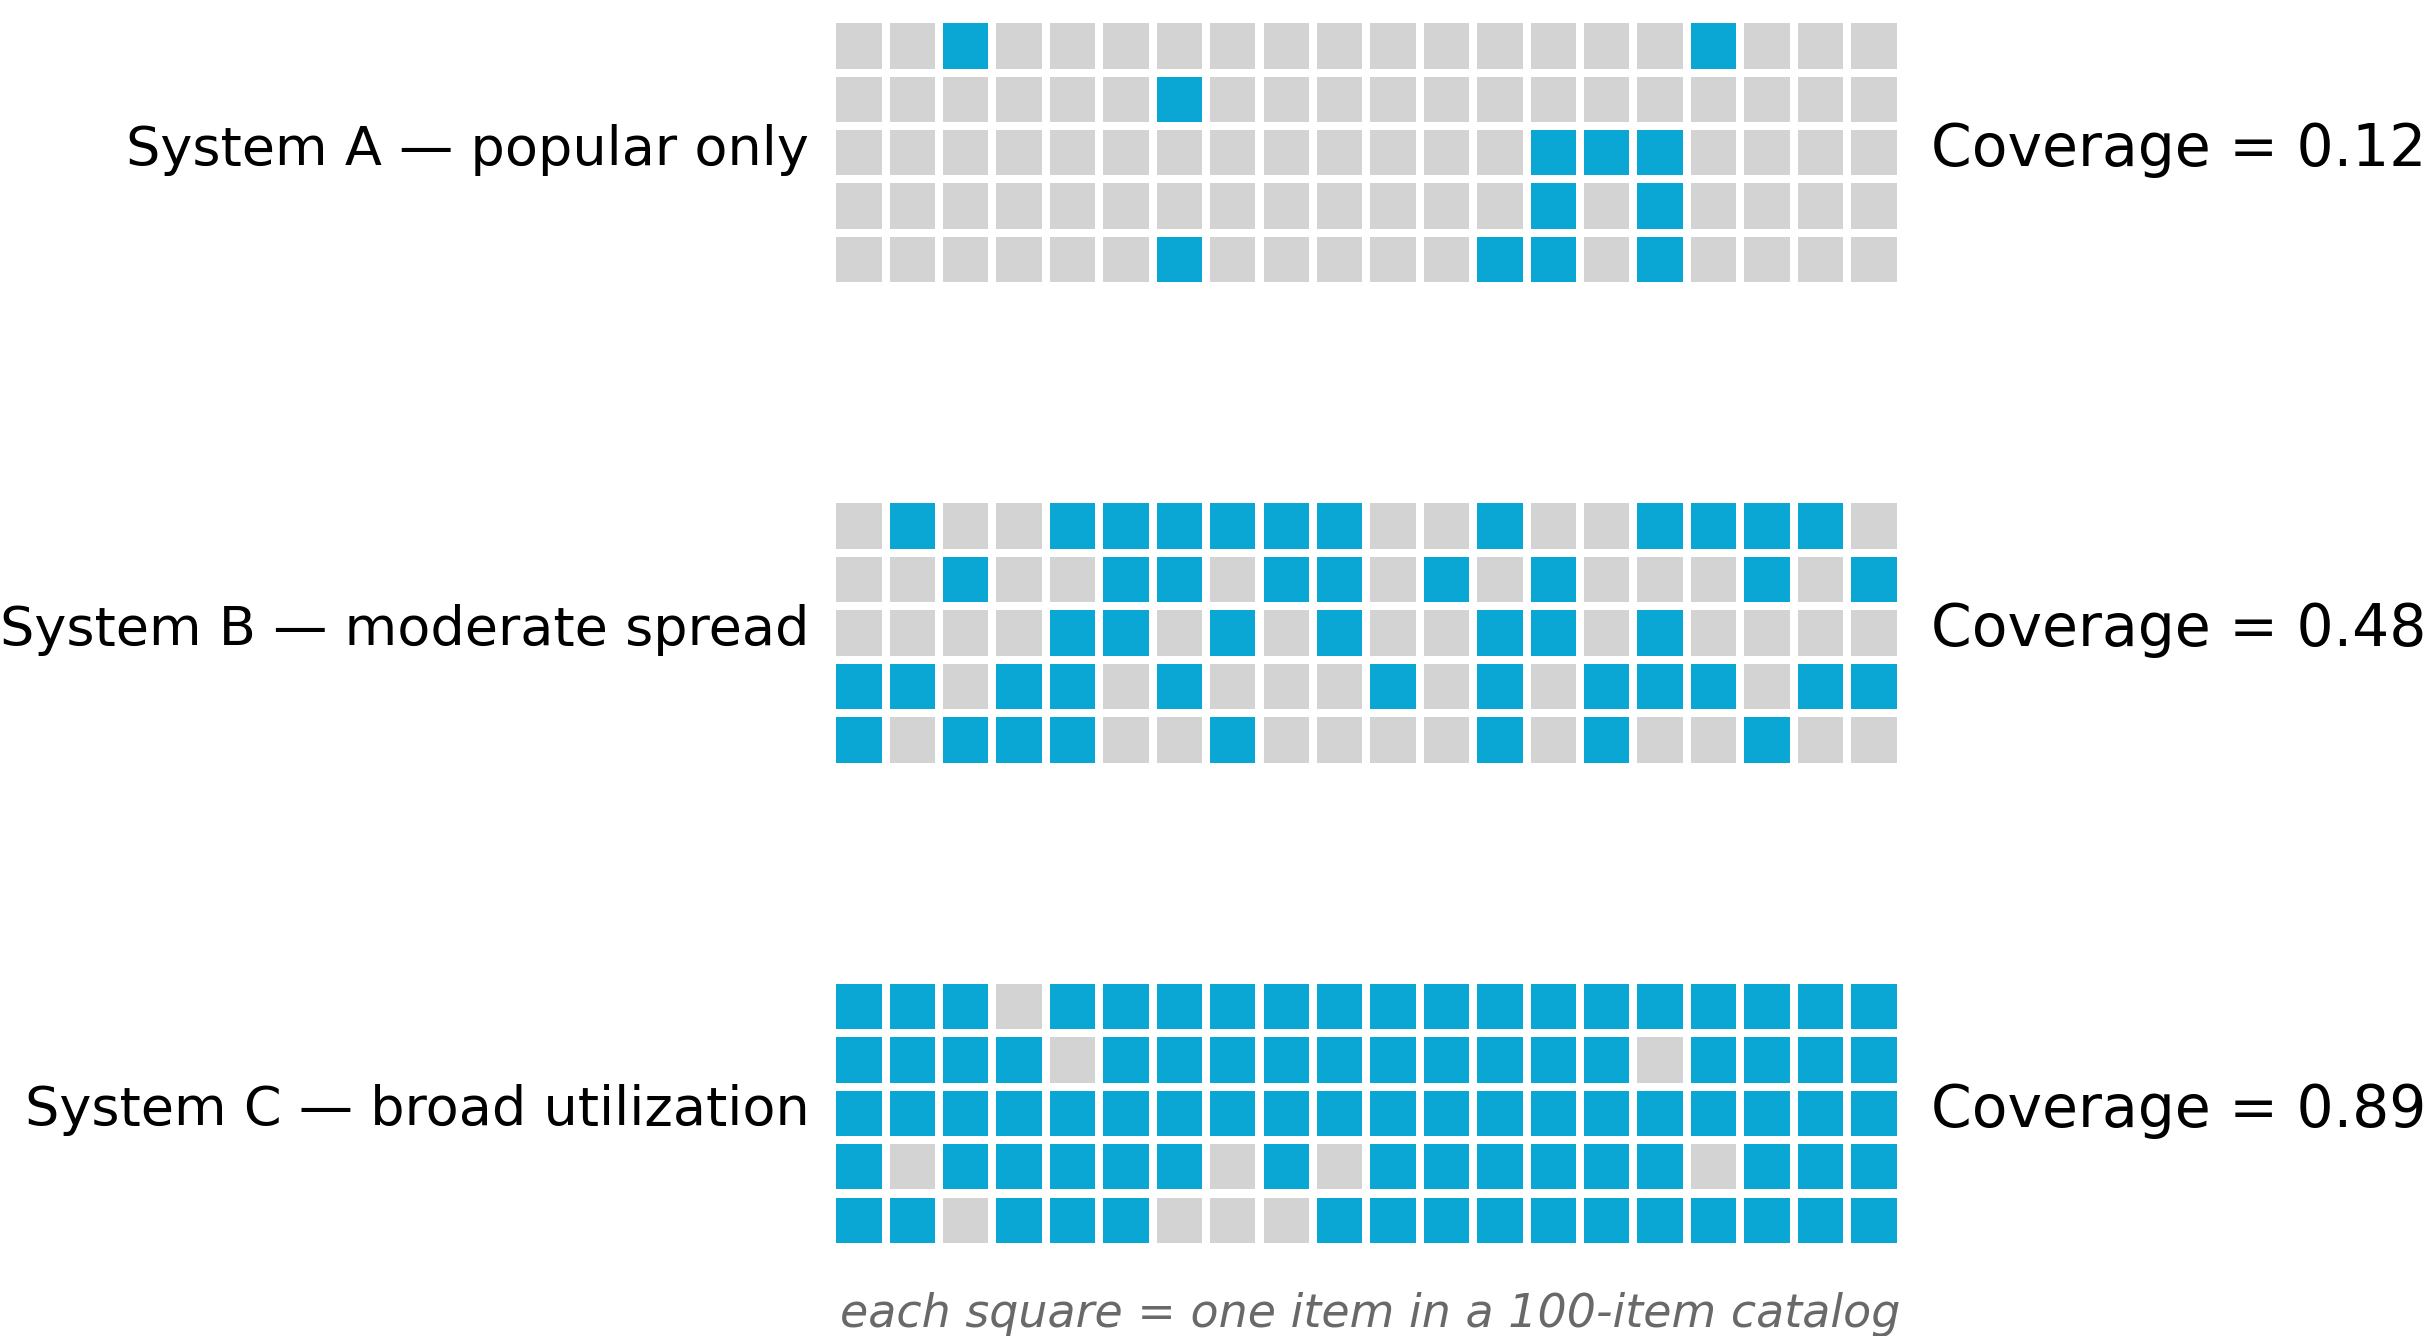
\includegraphics[width=0.6\textwidth]{figures/Coverage_comparison.png}
\end{figure*}

\textbf{Figure.} Three recommender systems with different coverage levels. System A only recommends popular items (12\% of catalog), while System C utilizes 89\% of the full catalog.

\orangebox{Did you know that...}
{Low coverage is a symptom of the "popularity bias" problem. Some recommender systems end up recommending the same small set of popular items
to all users, leaving the long tail of the catalog unexplored.}

\textbf{Other related metrics}

Coverage measures catalog breadth, while Diversity measures within-list variety. For measuring how new items are to individual users, see Novelty.
For accuracy-focused evaluation, use nDCG or MAP.
\include{6-computer-vision}
\chapteropener{NLP}{cyanhard}{cyanaccent}{%
Text has many correct answers, so most NLP metrics compare a candidate with one or more references by overlap. BLEU counts matching
n-grams with a precision bias and ROUGE with a recall bias; METEOR adds stems and synonyms and rewards contiguous matches; TER counts
the edits needed to reach the reference, and WER does the same for transcribed speech. Exact match is the strictest, for tasks with
one right span. All of them reward surface agreement and can punish a good paraphrase; the GenAI chapter picks up where they stop, with
metrics that compare meaning and distributions rather than tokens.}{In this chapter}


% ---------- Bilingual Evaluation Understudy ----------
\clearpage
\thispagestyle{nlpstyle}
\section{BLEU}
\subsection{Bilingual Evaluation Understudy}
% references:
% https://aclanthology.org/P02-1040.pdf



BLEU scores a machine translation by how much of its wording also appears in one or more human
references: it counts matching unigrams, then bigrams, trigrams, and 4-grams, and combines them.
A candidate that reuses the reference's exact phrasing scores near $1$; one that conveys the same
meaning in different words scores near $0$, because BLEU only sees surface overlap.

% equation
\begin{center}
    \tikz{
        \node[inner sep=2pt, font=\Large] (a) {
            {
                $\displaystyle
                BLEU = {\color{nmlred}BP} \cdot \exp\left(\sum_{n=1}^{N} {\color{nmlpurple}w_n} \log {\color{nmlcyan}p_n}\right)
                $
            }
        };
        \draw[overlay,-latex,nmlred, semithick] ($(a.south)+(-1.5,0.3)$) to[bend left=15] node[pos=1, left] {brevity penalty} +(-1,-.5);
        \draw[overlay,-latex,nmlcyan, semithick] ($(a.north)+(2.5,-0.2)$) to[bend left=15] node[pos=1, right] {n-gram precision} +(1,.5);
        \draw[overlay,-latex,nmlpurple, semithick] ($(a.south)+(1.0,0.3)$) to[bend right=15] node[pos=1, right] {n-gram weights} +(1,-.5);
    }
\end{center}

BLEU ranges from $0$ to $1$ (often reported $\times 100$) but only compares within a fixed tokenization
and reference set. The brevity penalty ${\color{nmlred}BP}$ stops a model from inflating precision by
emitting only the words it is most confident about.

\textbf{When to use BLEU?}

Use BLEU for machine translation and tasks with tight references, such as regression-testing quality
across model versions. Avoid it for open-ended generation where many wordings are valid (use METEOR or
BERTScore), and for single-sentence scoring, where its geometric mean is unstable --- BLEU is meant to be
averaged over a corpus.

\coloredboxes{
\item Fast, language-agnostic, and reproducible: scoring is just n-gram counting, so BLEU ranks
checkpoints in seconds with no model to run.
\item Correlates with human ranking at the corpus level --- which is why it became MT research's default
stopping signal, replacing a human eval after every change.
}
{
\item Blind to meaning. A correct paraphrase that shares no 4-grams with the reference scores near $0$,
the same as a wrong translation (see figure).
\item Sensitive to tokenization and casing. The same outputs can differ by several points; report
sacreBLEU (a standardized tokenization) for numbers comparable across papers.
}

\clearpage

\thispagestyle{customstyle}

\begin{center}
    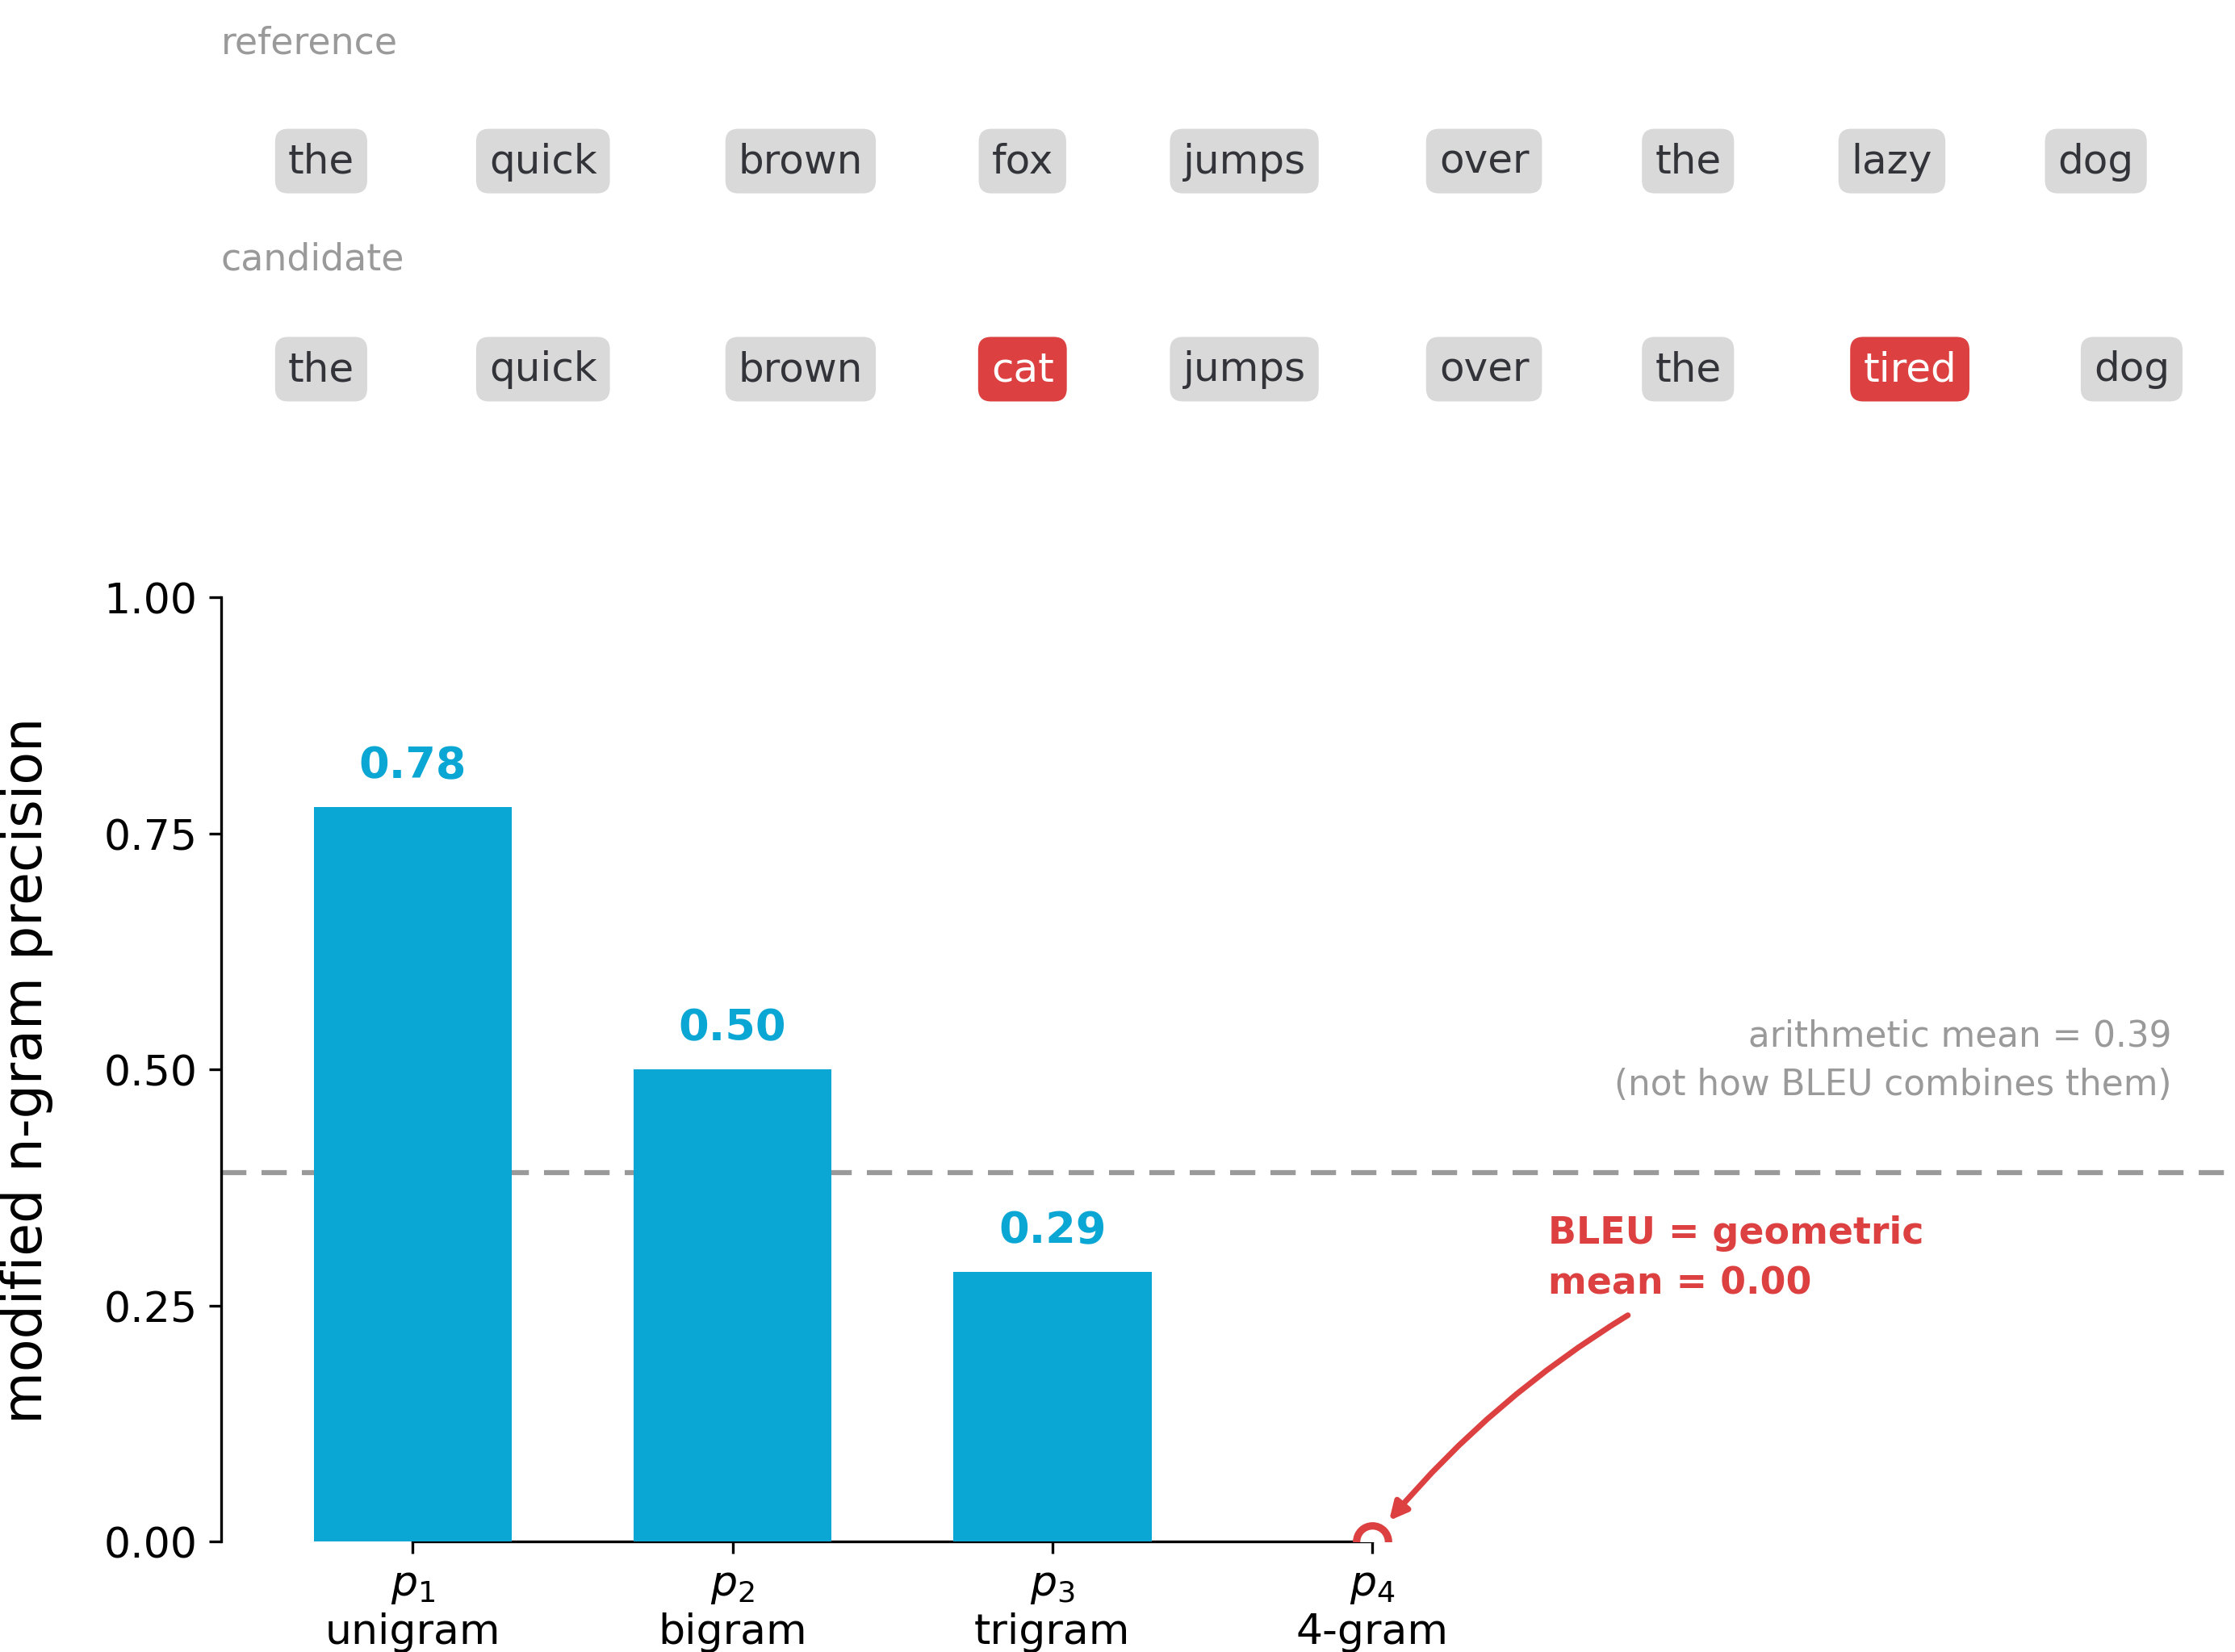
\includegraphics[width=0.62\textwidth]{figures/BLEU_ngram_precision.png}
\end{center}

\textbf{Figure. BLEU.} The candidate swaps two words, breaking every 4-gram, so the 4-gram precision $p_4$ is
$0$. Because BLEU is the geometric mean of the four precisions, that single zero drags the whole score
to $0$ --- even though $78\%$ of unigrams still match. An arithmetic mean would have reported $0.39$.
This is why sentence-level BLEU needs smoothing and is meant to be aggregated over a corpus.

\orangebox{Did you know that...}
{BLEU multiplies its n-gram precisions rather than averaging them: $\exp(\sum_n w_n \log p_n)$ is a
weighted \textbf{geometric} mean. The consequence is unforgiving --- if even one n-gram order has zero
matches, $\log 0 = -\infty$ and the whole score collapses to $0$, however good the lower orders are.
Introduced by Papineni et al. (2002) at IBM, BLEU was the first automatic MT metric to track human
judgment well enough to replace per-change human evaluation.}

\textbf{Other related metrics}

If BLEU is low but the translation reads correctly, the model is probably paraphrasing --- check METEOR
(credits synonyms and stems) or BERTScore (embedding similarity, see the GenAI chapter). TER reports the
same quality as an edit count rather than an overlap, and disagrees with BLEU on reordering, which it
penalizes more gently.

% ---------- Metric for Evaluation of Translation with Explicit ORdering ----------
% references:
% https://aclanthology.org/W05-0909.pdf

\clearpage
\thispagestyle{nlpstyle}
\section{METEOR}
\subsection{Metric for Evaluation of Translation with Explicit ORdering}

METEOR scores a translation the way a lenient grader would: it aligns the candidate to the reference
word by word, accepting not only exact matches but also stems (\textit{run}/\textit{running}) and
synonyms (\textit{quick}/\textit{fast}), then rewards how much of the reference it recovers. It exists
to fix the failure that hurts BLEU most --- a correct paraphrase worded differently. Where BLEU sees no
overlap and scores $0$, METEOR still credits the matched meaning.

% equation
\begin{center}
    \tikz{
        \node[inner sep=2pt, font=\Large] (a) {
            {
                $\displaystyle
                METEOR = (1 - {\color{nmlred}\gamma} \cdot {\color{nmlpurple}frag}^{\beta}) \cdot {\color{nmlcyan}F_{mean}}
                $
            }
        };
        \draw[overlay,-latex,nmlcyan, semithick] ($(a.north)+(2.5,-0.2)$) to[bend left=15] node[pos=1, right] {harmonic mean} +(1,.5);
        \draw[overlay,-latex,nmlpurple, semithick] ($(a.south)+(0.5,0.3)$) to[bend left=15] node[pos=1, left] {fragmentation penalty} +(-1,-.5);
    }
\end{center}

METEOR is the harmonic mean of unigram precision and recall (${\color{nmlcyan}F_{mean}}$), scaled down
by a fragmentation penalty (${\color{nmlred}\gamma}\cdot{\color{nmlpurple}frag}^{\beta}$) that grows as
matched words scatter out of order. It ranges from $0$ to $1$ and weights recall about nine times more
than precision, so recovering content matters more than staying terse.

\textbf{When to use METEOR?}

Use METEOR for translation and captioning when adequacy matters as much as exact wording, and for
morphologically rich or low-resource languages where exact n-gram matches are too strict. Avoid it when
you need cross-paper comparability (BLEU/sacreBLEU is standard) or when no stemmer or synonym resource
exists for your language --- the very thing that gives METEOR its edge.

\enlargethispage{\baselineskip}
\coloredboxes{
\item Credits synonyms and stems, so a fluent paraphrase scores near a literal translation --- exactly
where BLEU collapses to $0$ (see figure).
\item Correlates with human judgment at the \textit{sentence} level, not just the corpus level, because
precision, recall, and word order fold into one stable, recall-weighted score.
}
{
\item Needs linguistic resources. Stemmers and synonym tables (e.g.\ WordNet) must exist for the target
language; quality drops where they don't.
\item Slower and less standardized than BLEU. The alignment step and tunable parameters
($\alpha,\gamma,\beta$) mean two papers' METEOR numbers may not be comparable.
}

\clearpage

\thispagestyle{customstyle}

\begin{center}
    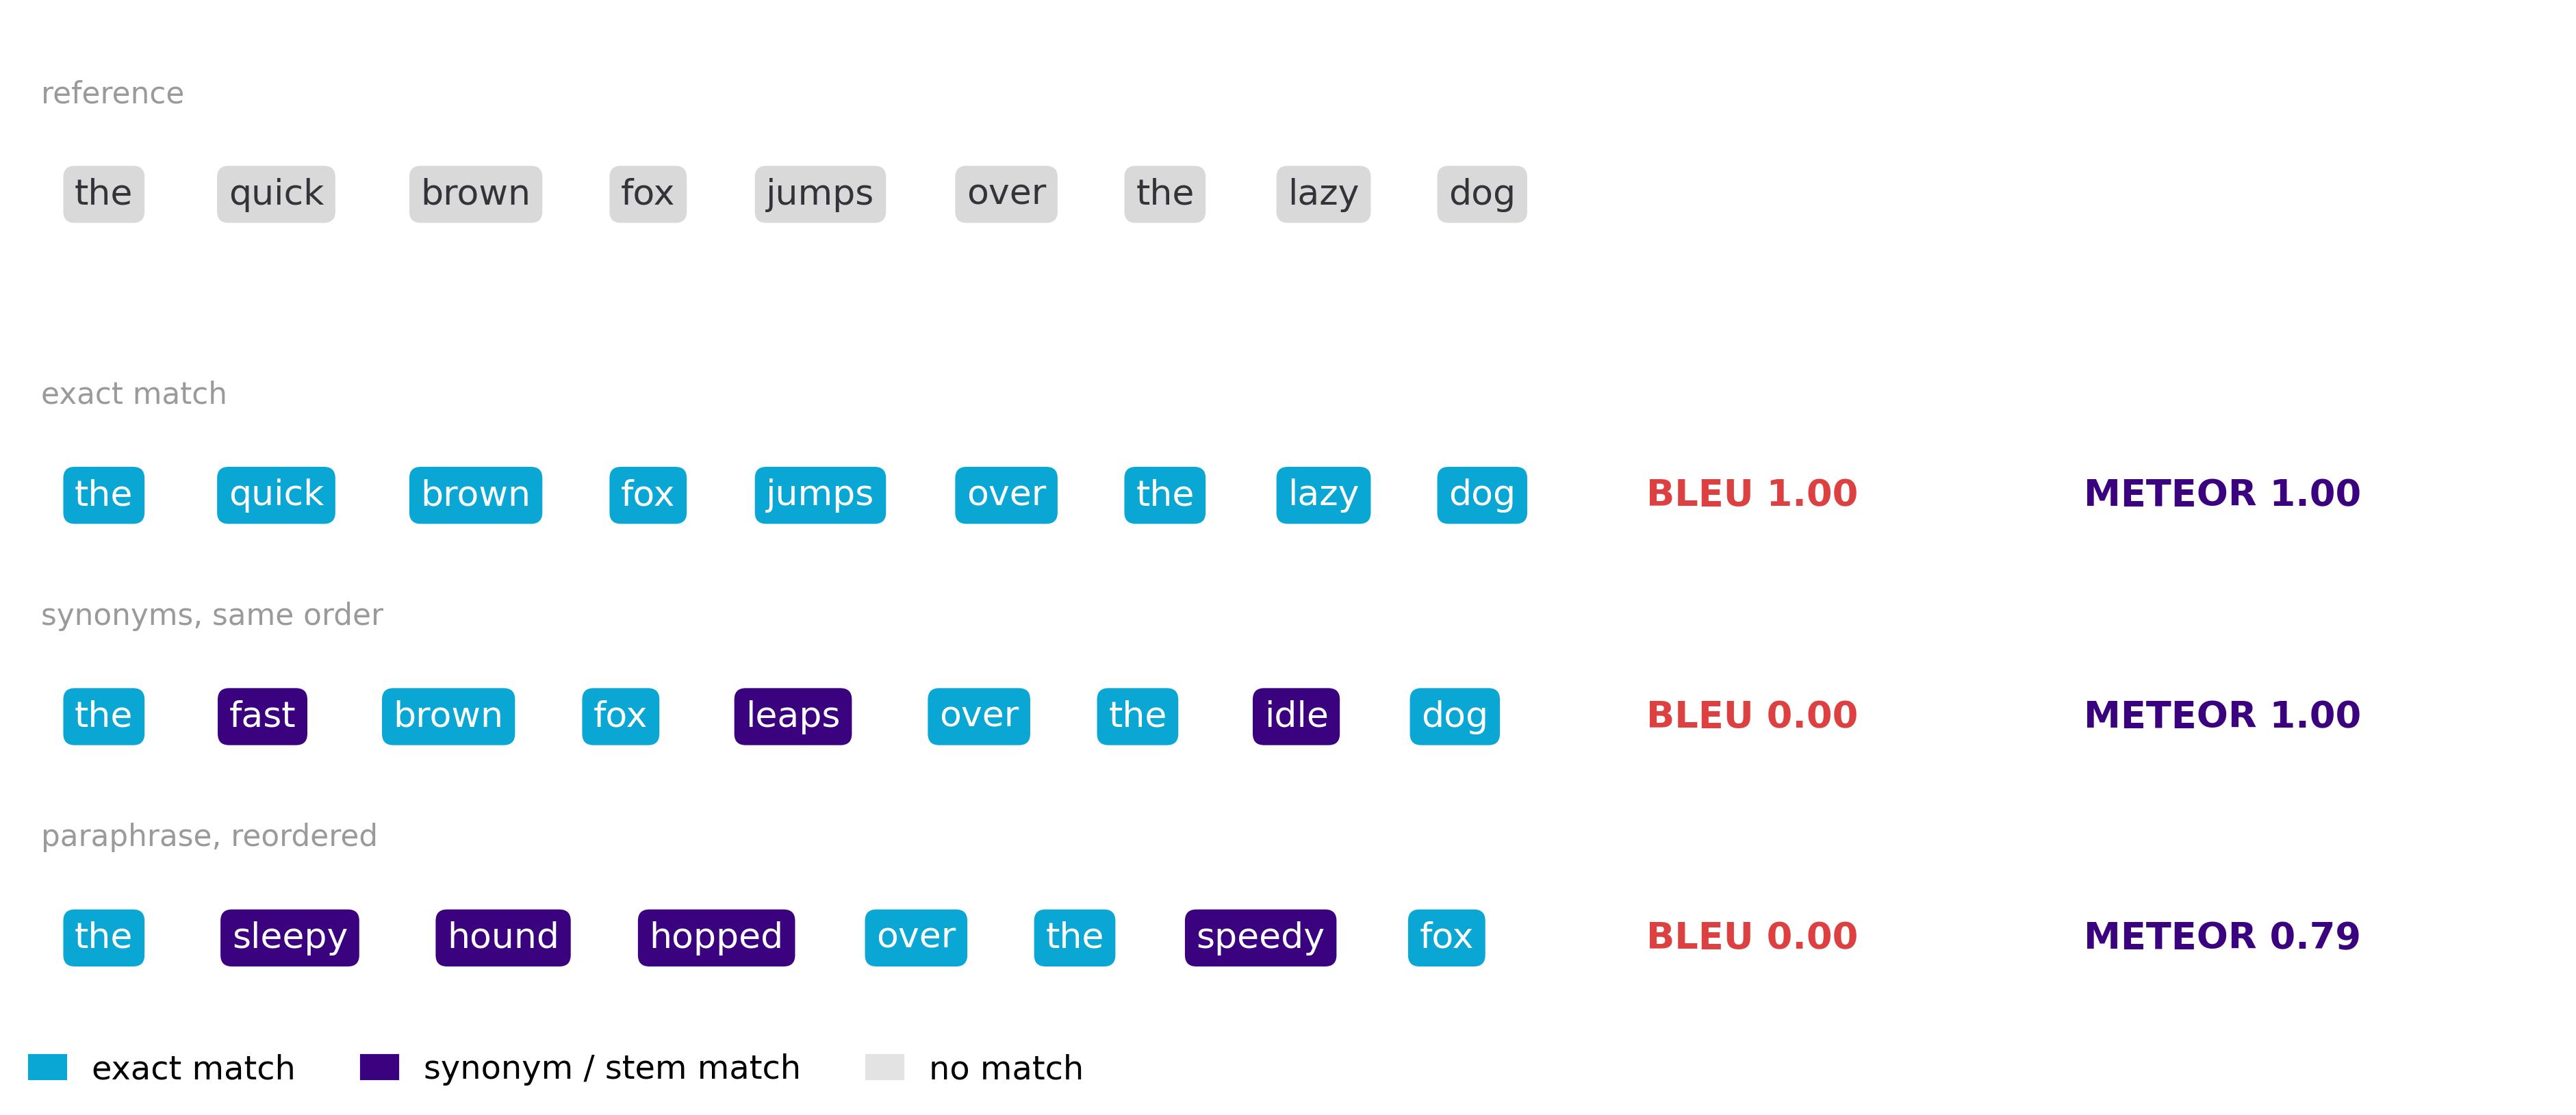
\includegraphics[width=\textwidth]{figures/METEOR_vs_BLEU.png}
\end{center}

\textbf{Figure. METEOR.} One reference scored against three candidates. Replacing words with synonyms
(\textit{fast}, \textit{leaps}, \textit{idle}) breaks every n-gram, so BLEU falls to $0$, but METEOR
matches them through its synonym and stem tables and stays at $1.0$. Reordering the paraphrase keeps the
matched words but scatters them, so METEOR's fragmentation penalty docks it to $0.79$ while BLEU again
reads $0$.

\orangebox{Did you know that...}
{METEOR's harmonic mean is deliberately unbalanced: $F_{mean} = \frac{P\cdot R}{\alpha P + (1-\alpha)R}$
with $\alpha = 0.9$, so recall carries nine times the weight of precision. A translation that recovers
all of the reference's meaning but adds a few words is barely penalized; one that drops content is hit
hard --- adequacy over brevity, by design. Developed at Carnegie Mellon (Banerjee \& Lavie, 2005) as a
direct response to BLEU.}

\textbf{Other related metrics}

A large METEOR--BLEU gap means the model is conveying the meaning with different words, not making
errors --- the paraphrase case BLEU cannot see. For a surface edit-based view compare TER; for
embedding-based similarity that needs no synonym table, see BERTScore in the GenAI chapter.

% ---------- Recall-Oriented Understudy for Gisting Evaluation ----------
% references:
% https://aclanthology.org/W04-1013.pdf
% https://aclanthology.org/E17-2007.pdf

\clearpage
\thispagestyle{nlpstyle}
\section{ROUGE}
\subsection{Recall-Oriented Understudy for Gisting Evaluation}

ROUGE evaluates a summary by how much of the reference it recovers: it counts overlapping unigrams
(ROUGE-1), bigrams (ROUGE-2), or the longest common subsequence (ROUGE-L), divided by the reference
total. It reports recall rather than precision because in summarization the risk is leaving content out,
not adding a little extra.

% equation
\begin{center}
    \tikz{
        \node[inner sep=2pt, font=\Large] (a) {
            {
                $\displaystyle
                ROUGE\text{-}N = \frac{\sum_{s \in Ref} \sum_{gram_n \in s} {\color{nmlcyan}Count_{match}}(gram_n)}{\sum_{s \in Ref} \sum_{gram_n \in s} {\color{nmlpurple}Count}(gram_n)}
                $
            }
        };
        \draw[overlay,-latex,nmlcyan, semithick] ($(a.north)+(2.0,-0.1)$) to[bend left=15] node[pos=1, right] {matching n-grams} +(1,.5);
        \draw[overlay,-latex,nmlpurple, semithick] ($(a.south)+(2.0,0.3)$) to[bend left=15] node[pos=1, left] {total reference n-grams} +(-1,-.5);
    }
\end{center}

ROUGE ranges from $0$ to $1$; the variant matters more than the absolute number. ROUGE-1 captures content
overlap, ROUGE-2 local fluency (word pairs), and ROUGE-L in-order overlap. Report ROUGE-1 and ROUGE-L
together --- a high ROUGE-1 with a low ROUGE-L means the right words in the wrong order.

\textbf{When to use ROUGE?}

Use ROUGE for summarization and tasks scored against reference text where coverage is the priority
(headline generation, extractive QA). Avoid recall-only ROUGE when verbosity matters --- a padded summary
keeps full recall while precision collapses (see figure); report ROUGE-F or a length budget instead. For
meaning over wording, use BERTScore.

\enlargethispage{\baselineskip}
\coloredboxes{
\item Cheap and reproducible: pure n-gram counting, scaling to thousands of summaries with no model to run.
\item The variant set is diagnostic --- ROUGE-1 vs ROUGE-2 vs ROUGE-L localizes a gap to content, local
fluency, or ordering.
}
{
\item Recall-only by default rewards length: a summary that copies the whole document earns near-perfect
recall, and only precision (usually unreported) catches the padding (see figure).
\item Lexical, not semantic. A correct abstractive paraphrase scores low; even human-written summaries
can score poorly under ROUGE.
}

\clearpage

\thispagestyle{customstyle}

\begin{center}
    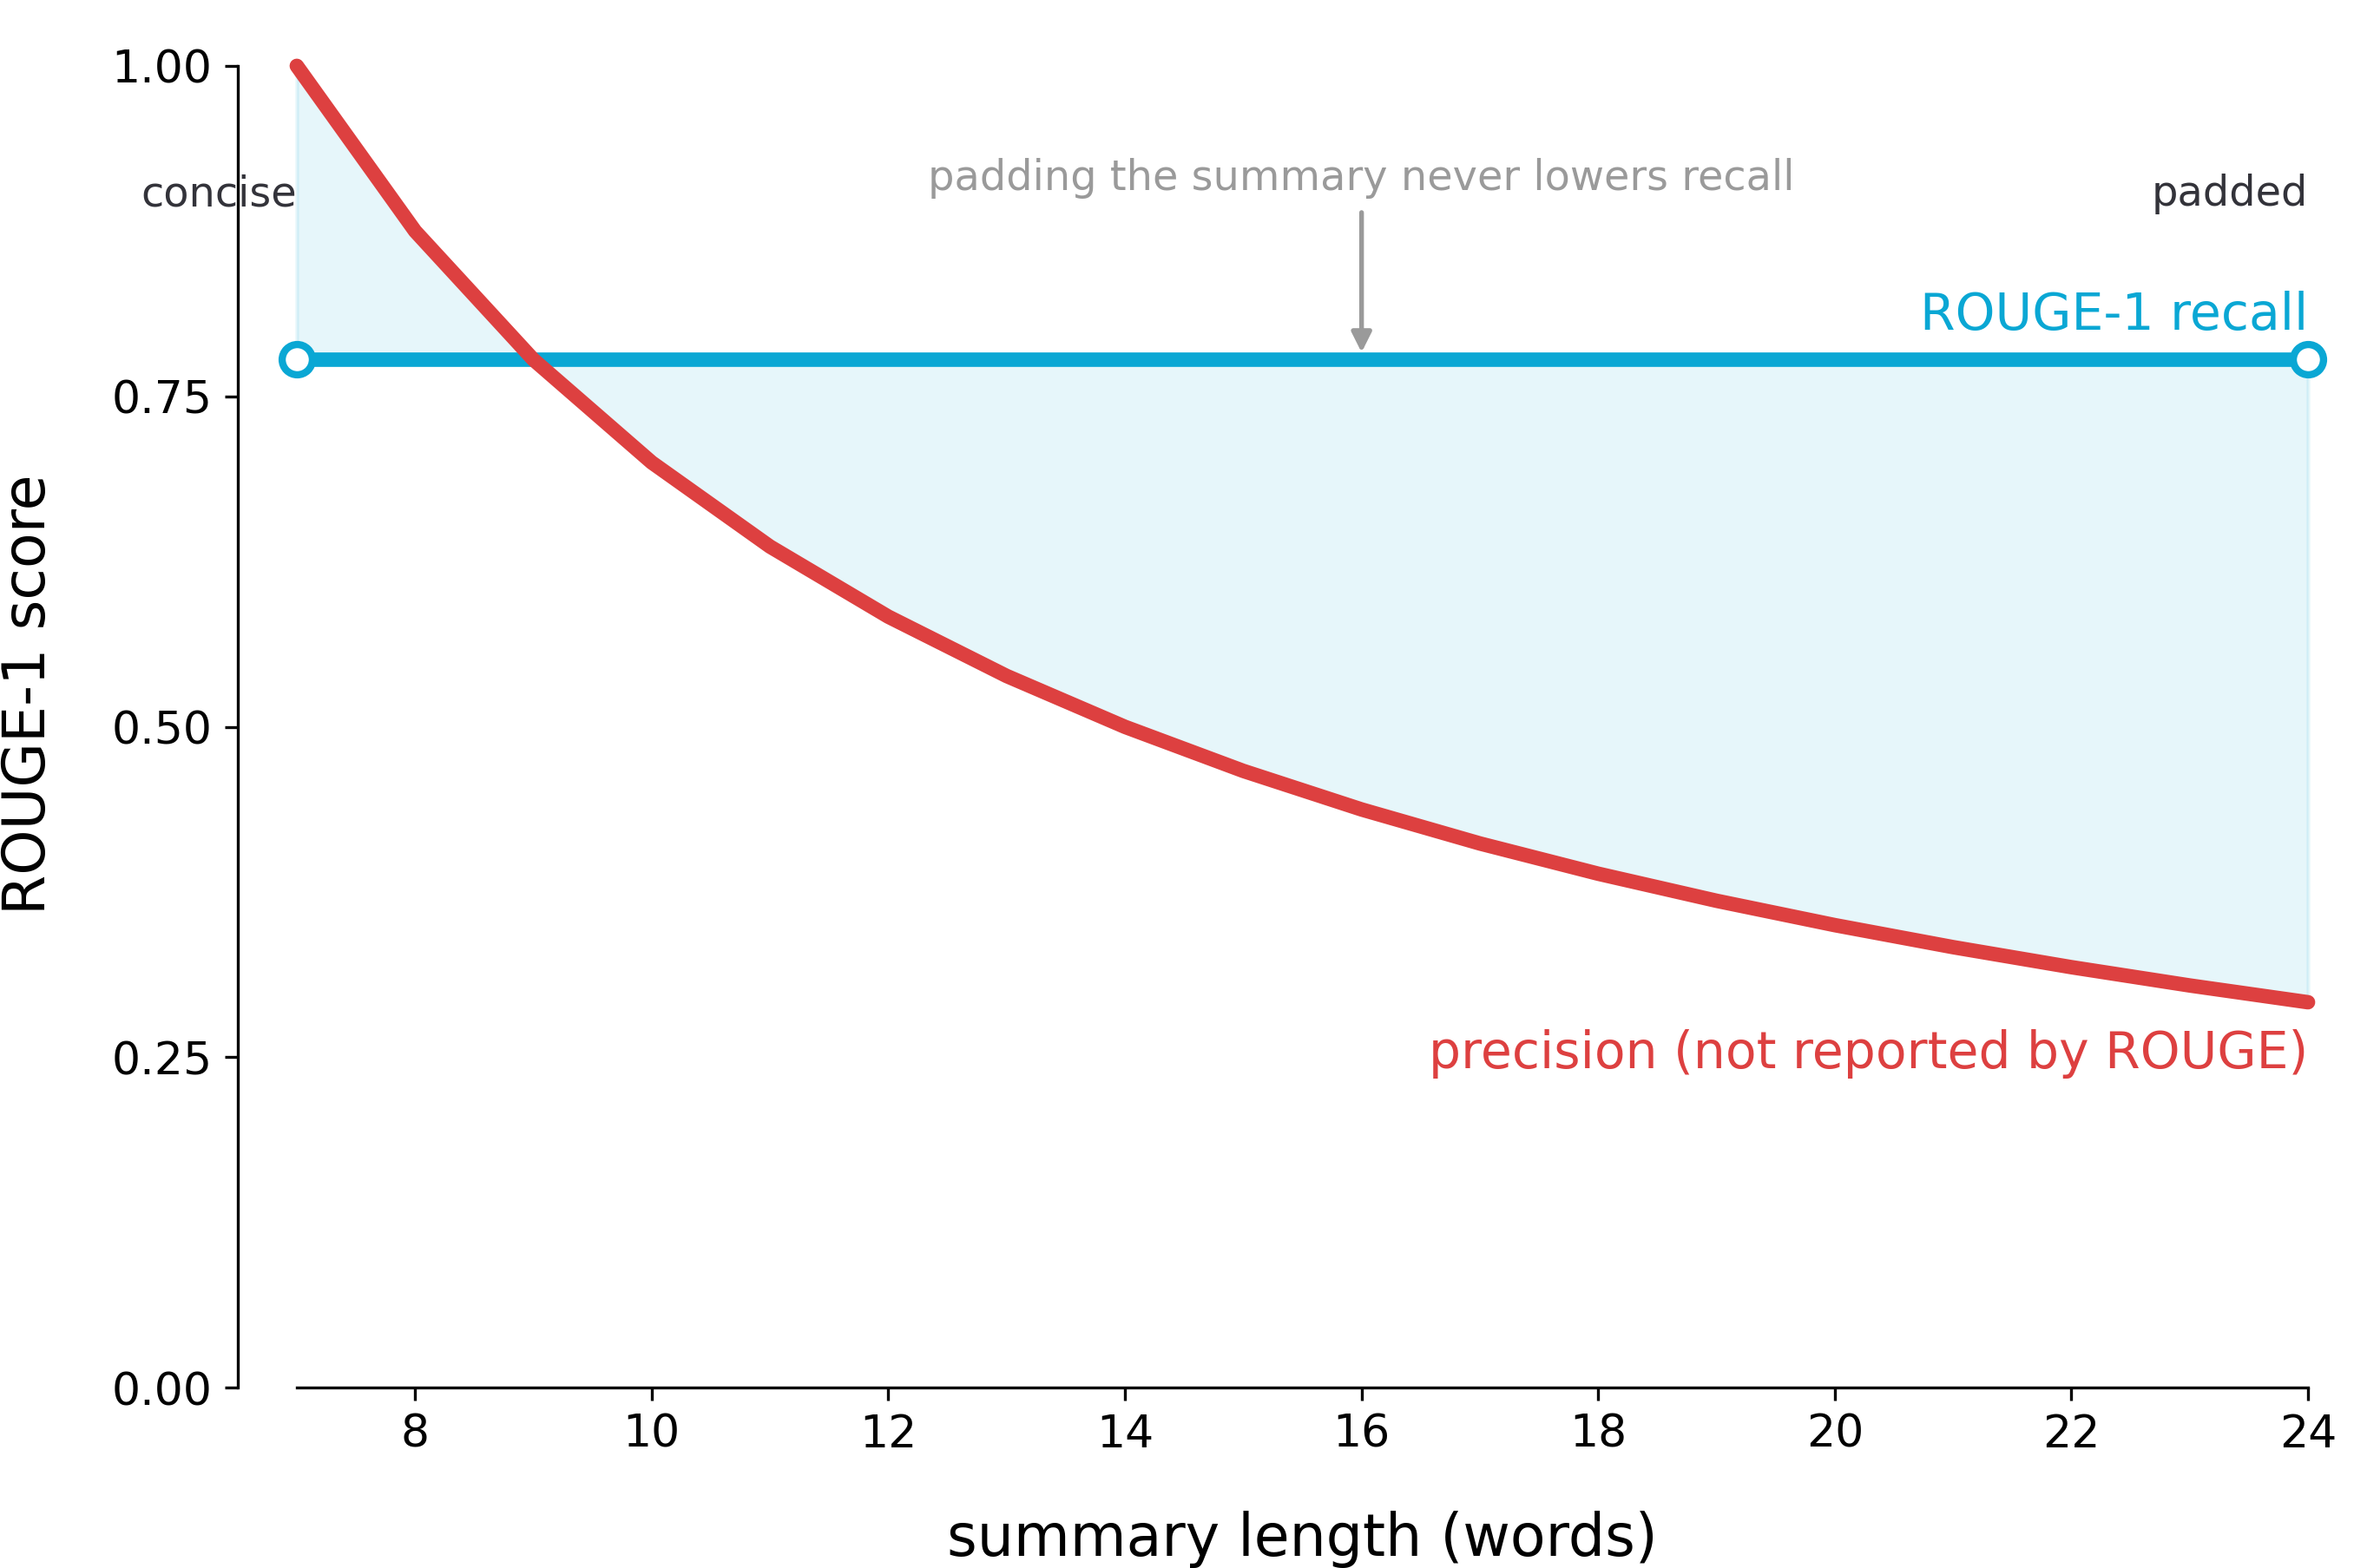
\includegraphics[width=0.6\textwidth]{figures/ROUGE_variants.png}
\end{center}

\textbf{Figure. ROUGE.} A concise summary already covers the reference, so its ROUGE-1 recall is $0.78$.
Appending filler words that aren't in the reference cannot lower recall --- it stays flat at $0.78$ ---
while precision falls from $1.0$ to $0.29$. Recall, the number ROUGE reports, is blind to padding; only
precision, which it omits, sees it.

\orangebox{Did you know that...}
{Because plain ROUGE is recall, it can only rise or stay flat as a summary grows: extra words never
remove a reference match, they only add chances for new ones. A system that emits the entire source
document scores near-perfect ROUGE recall while being useless as a summary --- which is why leaderboards
pair ROUGE with a length limit or report the F-score. Introduced by Chin-Yew Lin (2004); the name stands
for Recall-Oriented Understudy for Gisting Evaluation.}

\textbf{Other related metrics}

ROUGE is the recall-shaped mirror of BLEU's precision: to penalize over-generation, BLEU or ROUGE-F is
the better lens. A high ROUGE-1 with a low ROUGE-2 or ROUGE-L flags right-content, wrong-order. For
credit beyond exact tokens, see BERTScore in the GenAI chapter.

% ---------- Translation Error Rate ----------
% reference: https://aclanthology.org/2006.amta-papers.25.pdf
\clearpage
\thispagestyle{nlpstyle}
\section{TER}
\subsection{Translation Error Rate}

TER reports translation quality as post-editing effort: the fraction of edits a human would need to turn
the machine output into the reference. It counts insertions, deletions, substitutions, and --- unlike
word-error metrics --- shifts, where a whole phrase moves to a new position. A TER of $0.2$ means roughly
one edit per five reference words; lower is better.

% equation
\begin{center}
    \tikz{
        \node[inner sep=2pt, font=\Large] (a) {
            {
                $\displaystyle
                TER = \frac{{\color{nmlcyan}\text{insertions}} + {\color{nmlcyan}\text{deletions}} + {\color{nmlcyan}\text{substitutions}} + {\color{nmlpurple}\text{shifts}}}{{\color{nmlred}\text{reference length}}}
                $
            }
        };
        \draw[overlay,-latex,nmlcyan, semithick] ($(a.north)+(0.0,-0.1)$) to[bend right=15] node[pos=1, left] {word-level edits} +(-1,.5);
        \draw[overlay,-latex,nmlpurple, semithick] ($(a.north)+(2.7,-0.1)$) to[bend left=15] node[pos=1, right] {sequence shifts} +(0.0,.5);
        \draw[overlay,-latex,nmlred, semithick] ($(a.south)+(2.0,0.3)$) to[bend left=15] node[pos=1, left] {words in reference} +(-1,-.5);
    }
\end{center}

TER starts at $0$ (no edits) and can exceed $1$ when the output needs more edits than the reference has
words. Because it counts edits over reference length, TER reads directly as edits per reference word ---
which is why it tracks human post-editing time more closely than overlap scores.

\textbf{When to use TER?}

Use TER when the downstream cost is human post-editing: translation-memory pipelines, localization
vendors paid per edit. Its shift operation suits frequent reordering --- one moved phrase, one edit.
Avoid TER when correct paraphrases use different words (every substitution is an error; use METEOR or
BERTScore), and for leaderboards, where BLEU is the convention.

\enlargethispage{\baselineskip}
\coloredboxes{
\item Interpretable as work. A TER of $0.3$ estimates three edits per ten words --- a number a
localization manager can convert into hours and cost.
\item Handles reordering. The shift moves a whole phrase for one edit, so a correctly translated but
relocated clause isn't punished as several substitutions (see figure).
}
{
\item Surface-level. Different-but-correct word choices count as substitutions; TER has no notion of
synonymy.
\item Tends to overestimate effort. Its shift search is a greedy heuristic, not optimal, so it can
report more edits than a human would actually make.
}

\clearpage

\thispagestyle{customstyle}

\begin{center}
    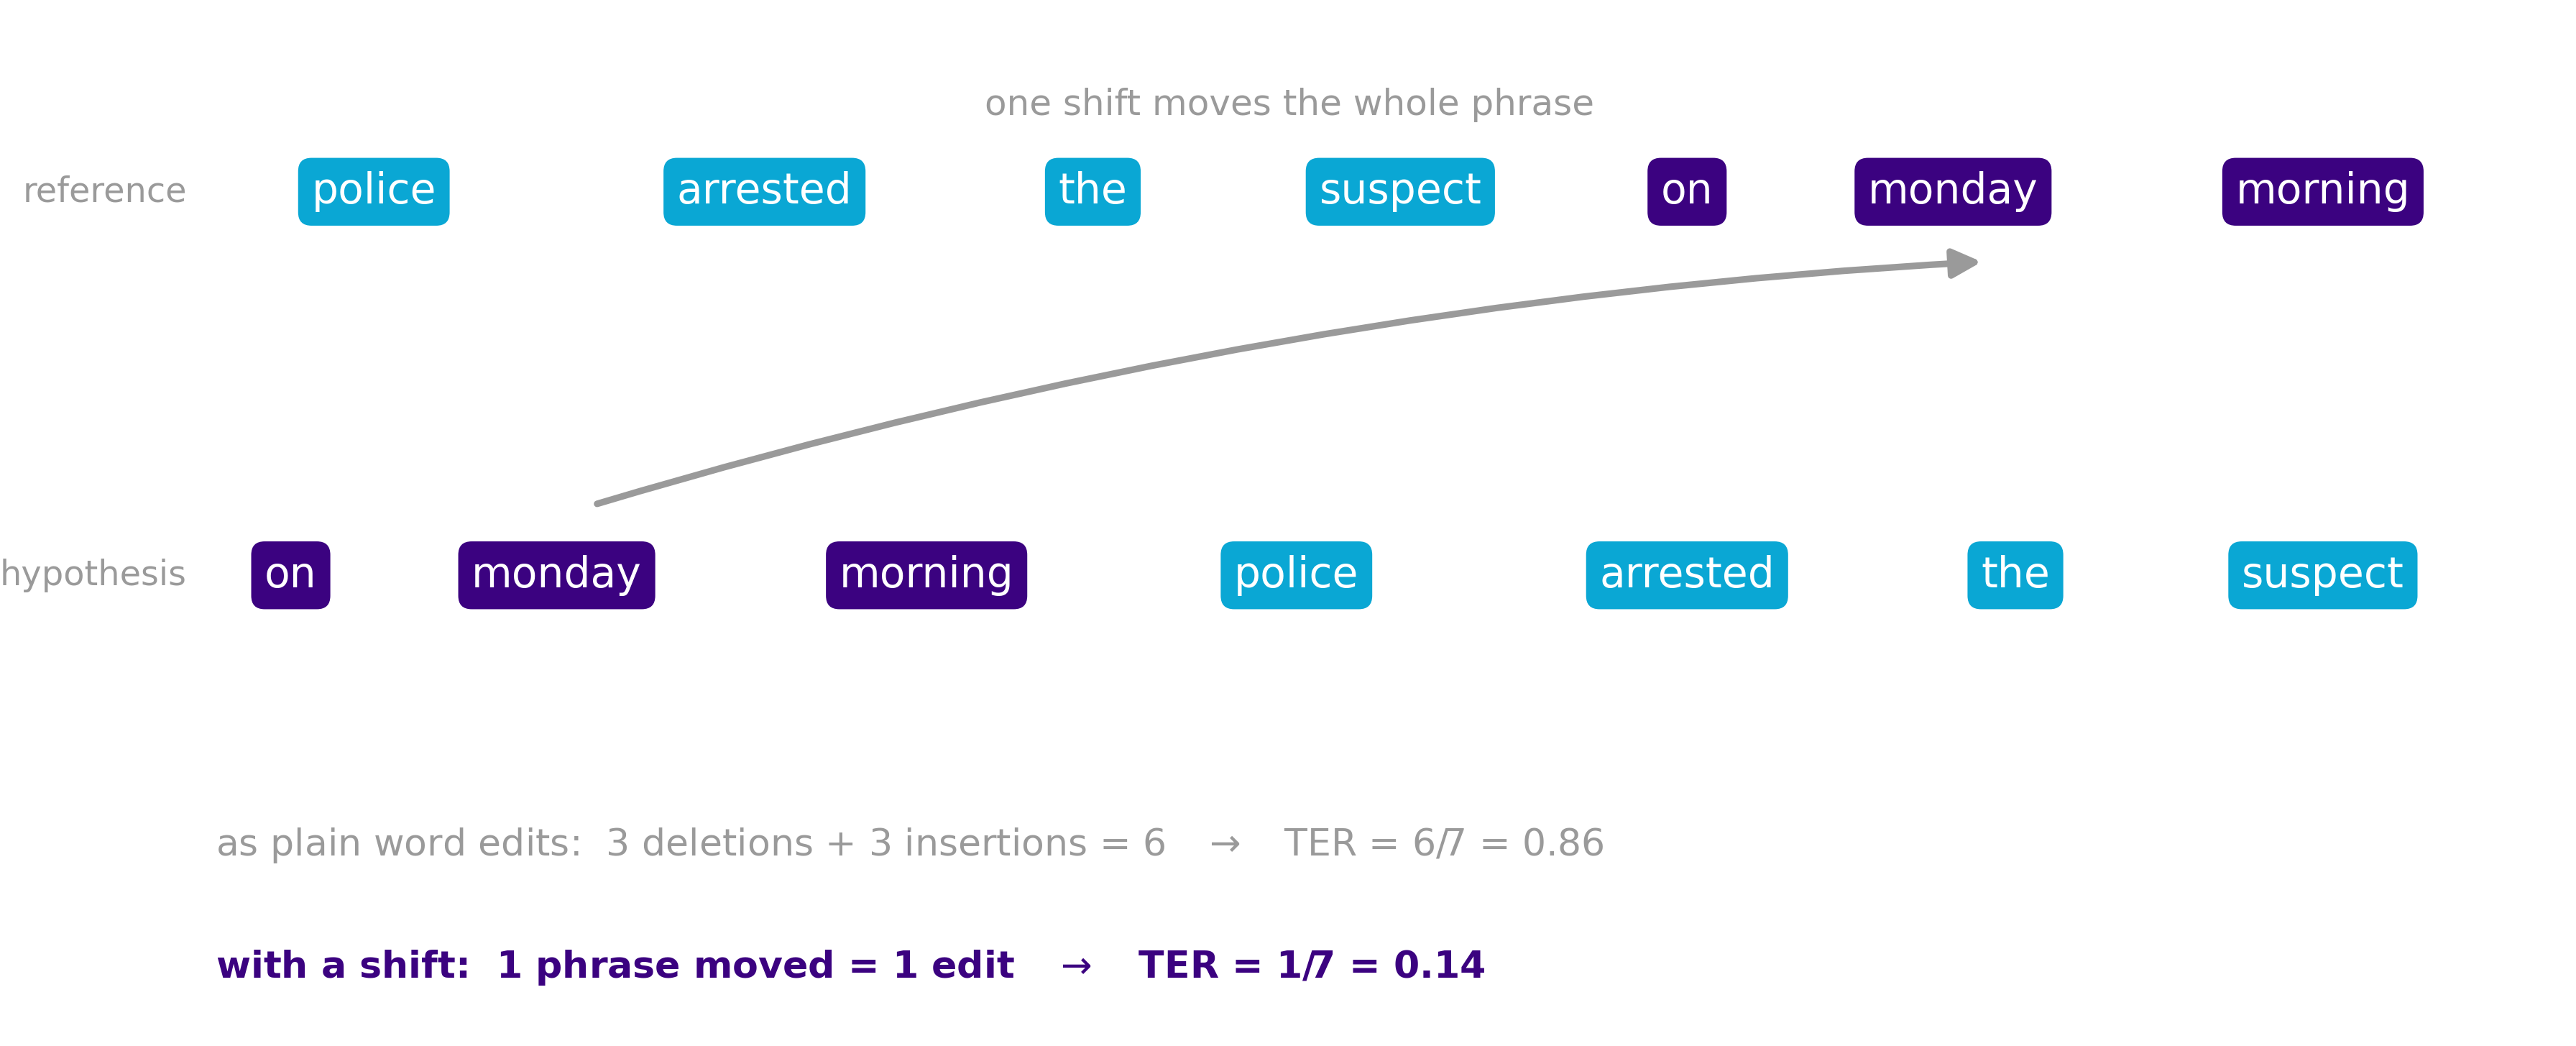
\includegraphics[width=\textwidth]{figures/TER_edit_breakdown.png}
\end{center}

\textbf{Figure. TER.} The hypothesis is the reference with the phrase \textit{on monday morning} moved to the
front. Scored as plain word edits, relocating the three-word phrase costs three deletions plus three
insertions ($\text{TER}=6/7=0.86$). TER's shift operation moves the whole phrase as a single edit
($\text{TER}=1/7=0.14$), matching the one drag a human editor would actually perform.

\orangebox{Did you know that...}
{The shift is what separates TER from word error rate. WER must delete every word of a misplaced phrase
and re-insert it elsewhere --- six edits for a three-word move --- so it punishes reordering harshly.
TER charges one edit for the move, whatever the phrase length or distance, because that mirrors the
single action a human takes. Finding the optimal set of shifts is expensive, so TER uses a greedy
approximation. Introduced by Snover et al.\ (2006).}

\textbf{Other related metrics}

TER and WER are the same edit-distance idea; TER adds the shift, so on reordered output TER is far lower
than a WER-style count. Against BLEU it often ranks systems differently, forgiving the reordering that
BLEU's n-grams punish. Lower TER is better --- the opposite direction to BLEU and METEOR.

% ---------- Exact Match ----------
% reference: https://nlp.stanford.edu/pubs/rajpurkar2016squad.pdf
\clearpage
\thispagestyle{nlpstyle}
\section{EM}
\subsection{Exact Match}

Exact Match is the fraction of predictions identical to the reference: each scores $1$ if it matches the
gold answer exactly --- after light normalization (lowercasing, stripping punctuation and articles) ---
and $0$ otherwise. It is the strictest text metric: \textit{Martin Luther King Jr.} scores $0$ against
the gold \textit{Martin Luther King}, the same score as a completely wrong answer (see figure).

% equation
\begin{center}
    \tikz{
        \node[inner sep=2pt, font=\Large] (a) {
            {
                $\displaystyle
                EM = \frac{1}{{\color{nmlred}N}} \sum_{i=1}^{N} {\color{nmlgreen}\mathds{1}}({\color{nmlpurple}\hat{y}_i} = {\color{nmlcyan}y_i})
                $
            }
        };
        \draw[overlay,-latex,nmlred, semithick] ($(a.south)+(-0.5,0.2)$) to[bend left=15] node[pos=1, left] {number of samples} +(-1,-.5);
        \draw[overlay,-latex,nmlpurple, semithick] ($(a.north)+(1.0,-0.2)$) to[bend right=15] node[pos=1, left] {predicted text} +(-1,.5);
        \draw[overlay,-latex,nmlcyan, semithick] ($(a.north)+(1.9,-0.2)$) to[bend left=15] node[pos=1, right] {reference text} +(1,.5);
    }
\end{center}

EM ranges from $0$ to $1$. Being all-or-nothing per example, it is most informative when the answer is
short and canonical; on long outputs it sits near $0$ even for good predictions, so it is usually paired
with token-level F1, which scores partial word overlap.

\textbf{When to use EM?}

Use EM where only an exact answer is acceptable: extractive QA spans, structured outputs (JSON keys, SQL,
API arguments), classification cast as text. Avoid it for open-ended or long-form generation, where it
bottoms out near $0$ even for strong outputs --- use token-F1, ROUGE, or BERTScore for graded credit.

\enlargethispage{\baselineskip}
\coloredboxes{
\item Unambiguous and trivial to explain: the prediction is either right or wrong, with no threshold to
tune.
\item Strict correctness guarantee. When any deviation breaks downstream use --- a malformed JSON key, a
wrong SQL clause --- EM is exactly the bar that matters.
}
{
\item All-or-nothing. A prediction off by one token scores $0$, identical to a fully wrong one:
\textit{Martin Luther King Jr.} and \textit{Malcolm X} both score $0$ against the gold (see figure).
\item Normalization-sensitive. Whether casing, punctuation, and articles are stripped before comparison
can swing EM by several points, so the scheme must be reported.
}

\clearpage

\begin{center}
    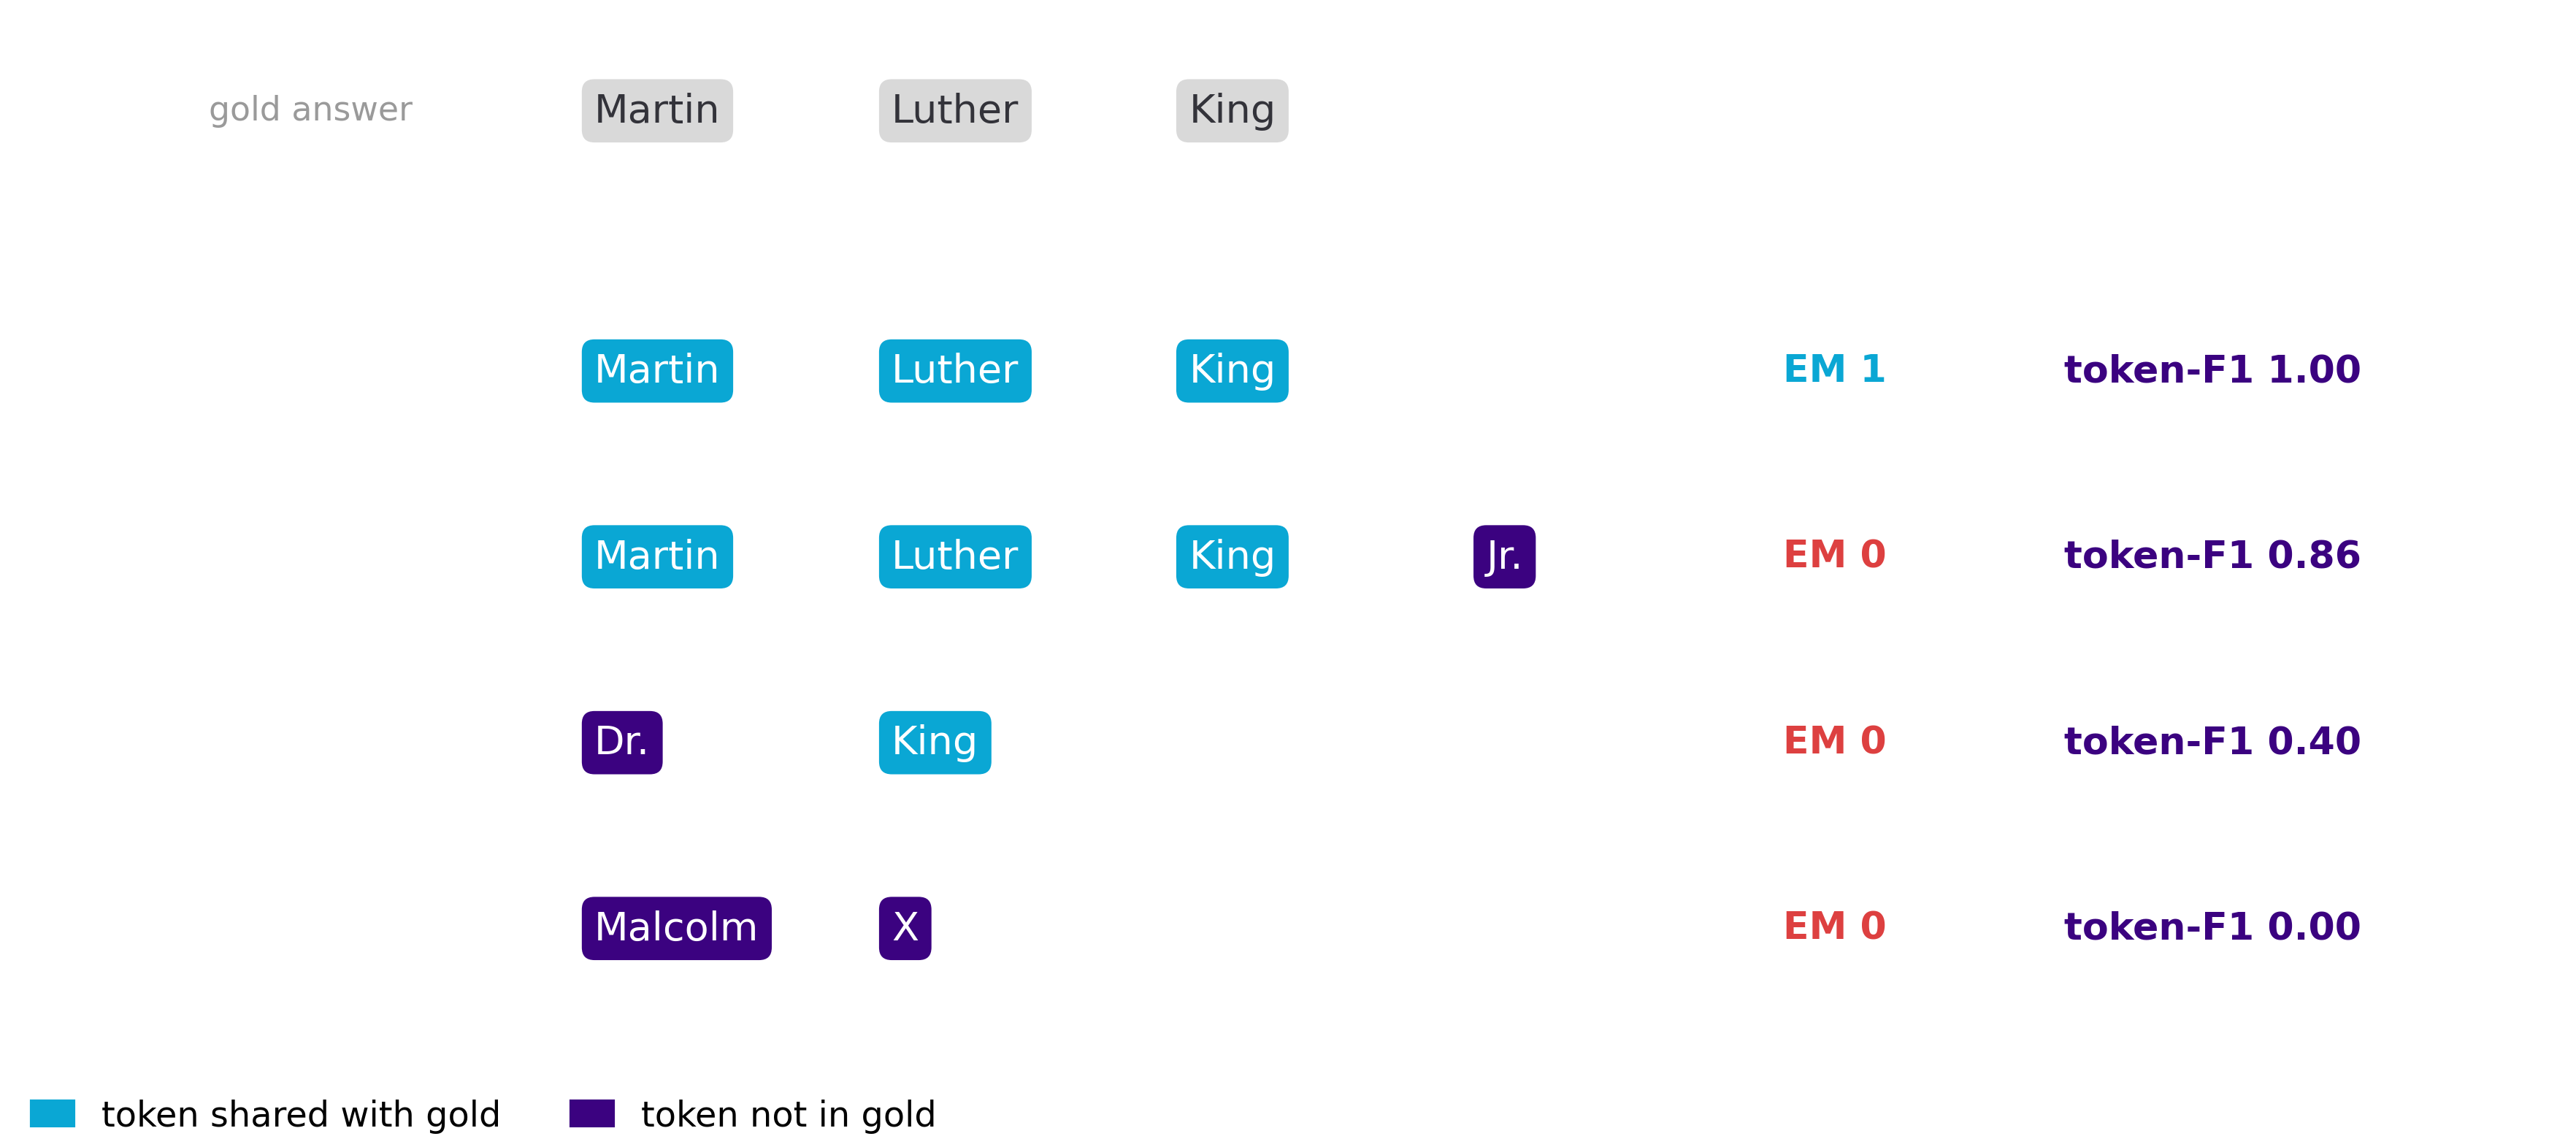
\includegraphics[width=0.95\textwidth]{figures/EM_vs_F1.png}
\end{center}

\textbf{Figure. EM.} Four predictions against the gold answer \textit{Martin Luther King}. Only the exact
match scores EM $=1$; adding \textit{Jr.}, abbreviating to \textit{Dr.\ King}, or answering
\textit{Malcolm X} all score EM $=0$. Token-level F1 instead grades the overlap --- $0.86$, $0.40$,
$0.00$ --- giving the partial credit EM withholds.

\orangebox{Did you know that...}
{Exact Match anchors the Stanford Question Answering Dataset (SQuAD) benchmark, always paired with
token-level F1. Token-F1 treats each answer as a bag of words and takes the harmonic mean of how many
predicted tokens appear in the gold answer (precision) and how many gold tokens were recovered (recall)
--- so \textit{Martin Luther King Jr.} earns F1 $=0.86$ for its three correct tokens while EM gives it
nothing. EM reports exact correctness; F1 reports how close the near-misses came.}

\textbf{Other related metrics}

EM and token-F1 are read together: a large F1--EM gap means the model is almost right --- correct
content, wrong boundaries or extra words --- rather than wrong. For n-gram overlap on longer text, see
BLEU or ROUGE; for semantic equivalence, BERTScore.

% ---------- Word Error Rate ----------
\clearpage
\thispagestyle{nlpstyle}
\section{WER}
\subsection{Word Error Rate}

WER scores a speech recognizer by how many word-level edits separate its transcript from the reference:
count the substitutions, deletions, and insertions in the best alignment, then divide by the number of
reference words. A WER of $0.1$ means one word in ten is wrong. It is the standard yardstick for ASR
because transcription errors are naturally counted in words.

% equation
\begin{center}
    \tikz{
        \node[inner sep=2pt, font=\Large] (a) {
            {
                $\displaystyle
                WER = \frac{{\color{nmlcyan}S} + {\color{nmlcyan}D} + {\color{nmlcyan}I}}{{\color{nmlred}N}}
                $
            }
        };
        \draw[overlay,-latex,nmlcyan, semithick] ($(a.north)+(0.5,-0.1)$) to[bend right=15] node[pos=1, left] {edit operations} +(-1,.5);
        \draw[overlay,-latex,nmlred, semithick] ($(a.south)+(1.0,0.2)$) to[bend left=15] node[pos=1, left] {words in reference} +(-1,-.5);
    }
\end{center}

WER starts at $0$ and can exceed $1$ ($100\%$) when a transcript inserts more wrong words than the
reference has. The three error types are diagnostic on their own: many insertions point to a decoder that
hallucinates words, many deletions to dropped speech, substitutions to confusable words (see figure).

\textbf{When to use WER?}

Use WER for ASR, voice assistants, and dictation, where every word should be transcribed correctly. Avoid
it when meaning survives the errors --- \textit{can't} versus \textit{cannot} is one substitution but no
change in meaning --- and for character-based or tonal languages, where Character Error Rate (CER), the
same formula per character, fits better.

\enlargethispage{\baselineskip}
\coloredboxes{
\item Diagnostic by construction. Splitting errors into substitutions, deletions, and insertions points
at the failure mode, not just its size (see figure).
\item Standard and interpretable. ``One word in ten wrong'' is understood across the field, making WER
comparable across systems and datasets.
}
{
\item Blind to meaning and importance. Every word counts equally: misrecognizing a critical digit and
dropping a filler ``um'' both cost one edit, though only one changes the message.
\item Sensitive to normalization. Punctuation, casing, contractions, and number formatting must be
standardized first, or formatting differences inflate WER with no real recognition error.
}

\clearpage

\begin{center}
    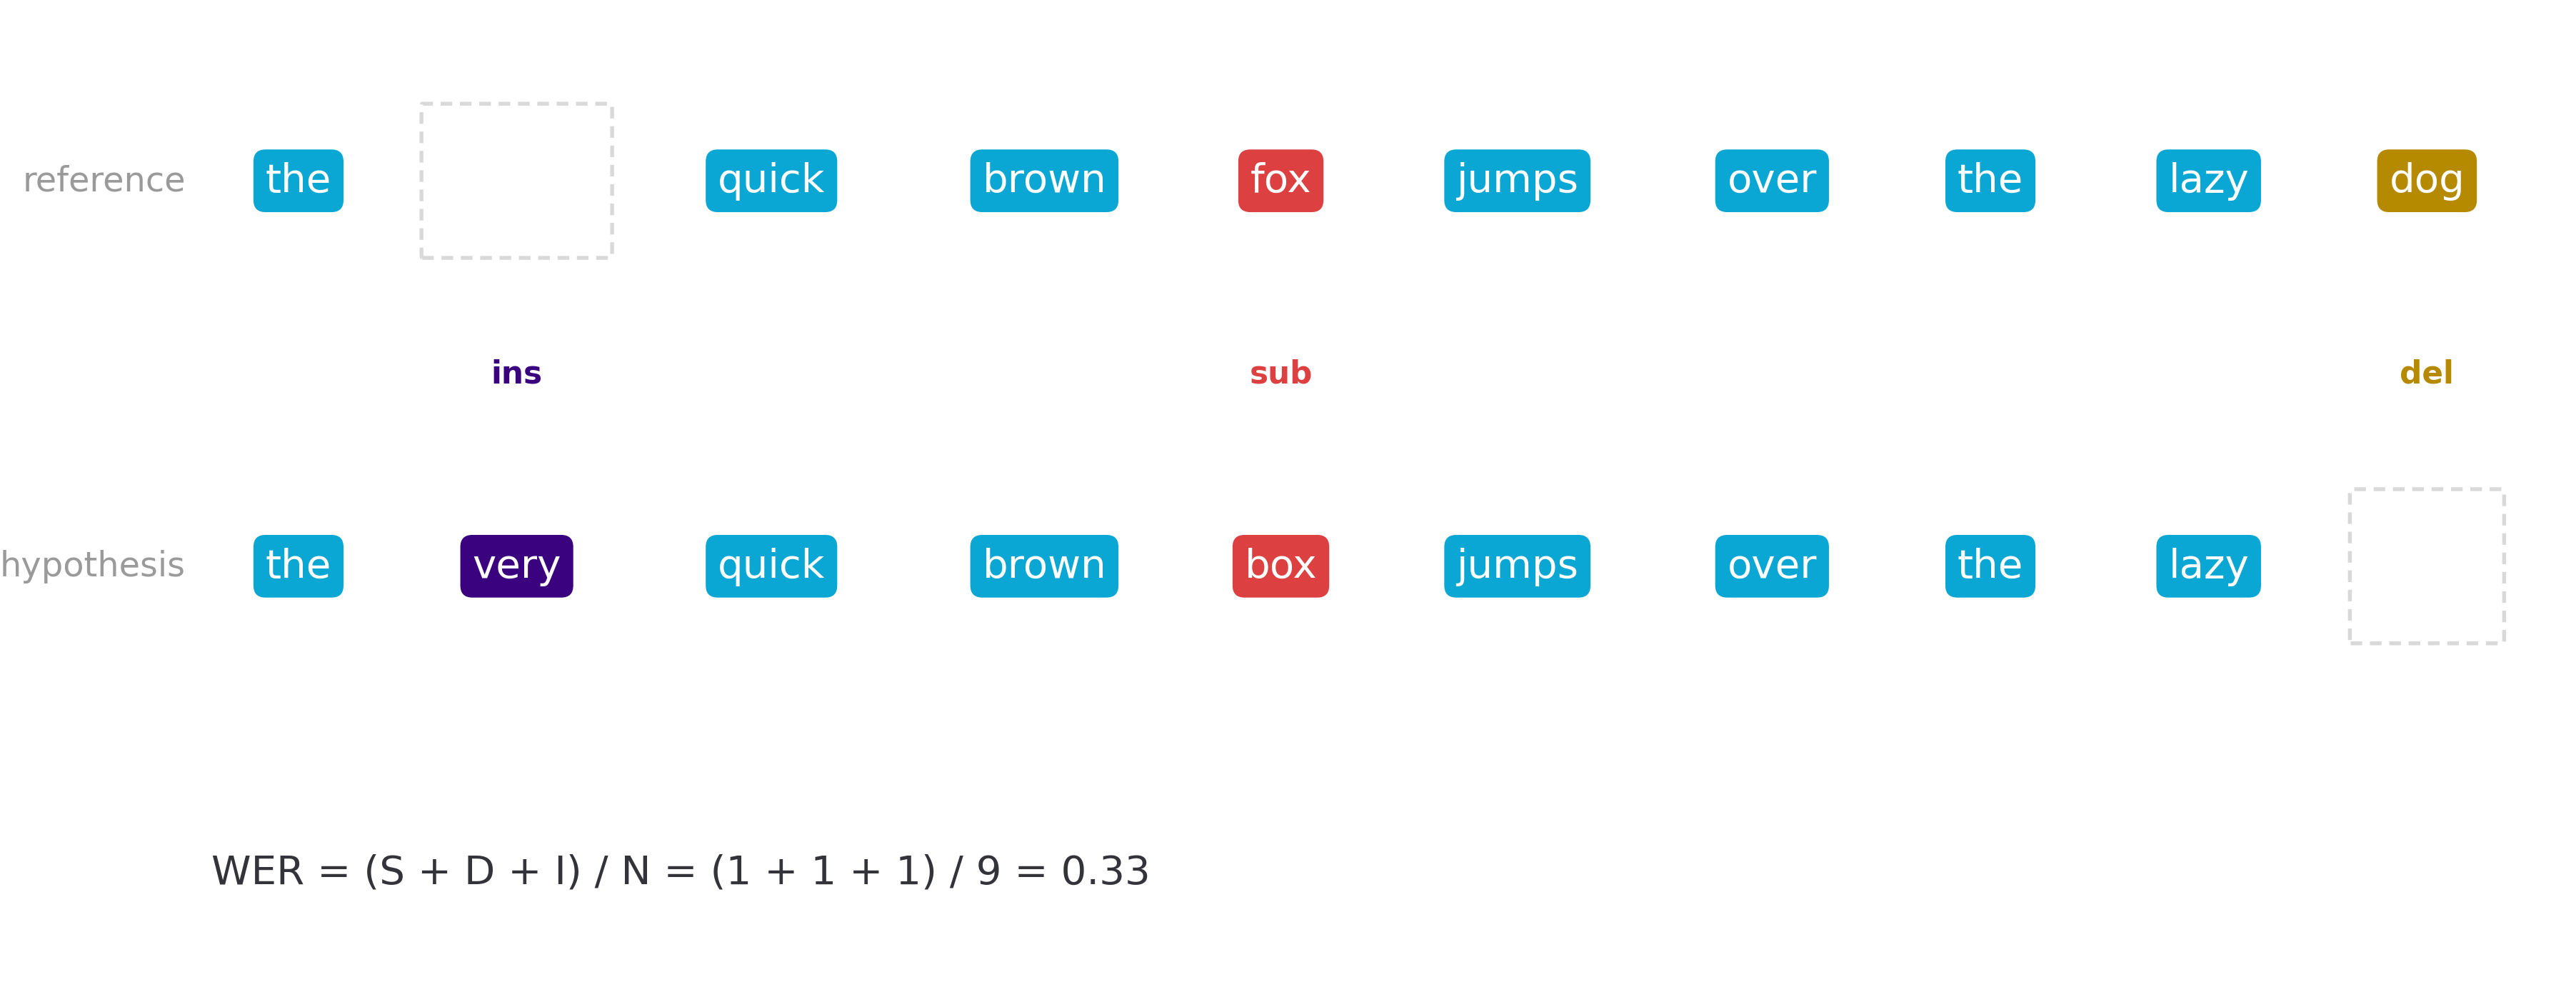
\includegraphics[width=\textwidth]{figures/WER_vs_errors.png}
\end{center}

\textbf{Figure. WER.} The best alignment between reference and hypothesis splits the errors into one
substitution (\textit{fox}\,$\rightarrow$\,\textit{box}), one deletion (\textit{dog}), and one insertion
(\textit{very}). WER sums them over the reference length: $(1+1+1)/9 = 0.33$. That same alignment is what
lets WER report \textit{which} kind of error dominates, not merely how many.

\orangebox{Did you know that...}
{WER is the Levenshtein (edit) distance computed over words instead of characters, normalized by the
reference length. The substitution, deletion, and insertion counts come from the \textit{minimum-cost}
alignment, found by dynamic programming --- so the split into error types is the cheapest explanation of
the differences, not the only one. Run the identical computation per character and you get Character
Error Rate (CER). The distance was introduced by Levenshtein in 1965.}

\textbf{Other related metrics}

WER and TER share the edit-distance core; TER adds a shift operation, so on reordered output (common in
translation, rare in transcription) TER reads far lower. For languages where word boundaries are unclear,
CER applies the identical formula per character. For meaning-level scoring beyond surface edits, see
BERTScore.
\include{8-genai}
\chapteropener{Probabilistic}{orangehard}{orangeaccent}{%
In this chapter, we check whether a model's probabilities match observed outcomes and estimate its performance before new labels
arrive. A loan model, for example, predicts repayment when someone applies, but we may wait months to learn whether they repay.
Earlier predictions and their outcomes can help us estimate performance during that wait.

Those earlier examples form a labeled \emph{reference dataset}. The estimator learns from their known outcomes, then estimates
performance for each new batch of predictions before its labels arrive. Each batch forms a \emph{chunk}
in the figures. We keep the reference examples separate from the monitored model's training data and validate the estimator on
held-out data.

Expected Calibration Error (ECE) measures \emph{calibration}: how well predicted probabilities agree with observed outcomes.
Two classification methods, CBPE and PAPE, then use calibrated probabilities to estimate metrics such as accuracy and F1.
For regression, Direct Loss Estimation (DLE) learns to predict the model's error.

These estimates can track changes in the input mix, or \emph{covariate shift}, but they assume the relationship between inputs
and outcomes stays the same. If that relationship changes, we have \emph{concept drift}. Once labels arrive, Reverse Concept
Drift (RCD) helps us estimate its effect on performance.}{In this chapter}

% ---------- Decision map ----------
\begin{decisionmap}{orangehard}{orangeaccent}{Which metric?}{Follow the branches to a method. The number next to it is its page.}
\maproot{Have the labels arrived?}
\begin{forest} dmap, large
[, coordinate, l sep=0pt
  [{\dl{yes: how much is concept drift?}{\mref{RCD}{sec:rcd}}}]
  [{\dm{no, and it is a classifier}{Are the reference probabilities calibrated?}}
    [{\dl{check that first}{\mref{ECE}{sec:ece}}}]
    [{\dl{calibration still holds in production}{\mref{CBPE}{sec:cbpe}}}]
    [{\dl{input mix changed; reference covers it}{\mref{PAPE}{sec:pape}}}]
  ]
  [{\dl{no, and it is a regressor}{\mref{DLE}{sec:dle}}}]
]
\end{forest}
\end{decisionmap}


% ---------- Expected Calibration Error ----------
\clearpage
\thispagestyle{probabilisticstyle}
\section{ECE}\label{sec:ece}
\subsection{Expected Calibration Error}

% reference:
% Naeini, Cooper, Hauskrecht (2015) — Obtaining Well Calibrated Probabilities Using Bayesian Binning
% Guo, Pleiss, Sun, Weinberger (2017) — On Calibration of Modern Neural Networks (temperature scaling)
% Murphy (1973) — decomposition of the Brier score

Expected Calibration Error measures the gap between a classifier's confidence and how often its predictions are correct. Here,
confidence means the probability assigned to the predicted class. If predictions made with about $80\%$ confidence are correct
only $70\%$ of the time, the model is overconfident in that range. ECE groups predictions into confidence bins and averages these
gaps, giving more weight to bins with more predictions.

% equation
\begin{center}
    \tikz{
        \node[inner sep=2pt, font=\Large] (a) {
            {
                $\displaystyle
                \text{ECE} = \sum_{b=1}^{B} \frac{{\color{nmlred}|B_b|}}{{\color{nmlred}n}} \,\Big|\, {\color{nmlcyan}\text{acc}}(B_b) - {\color{nmlpurple}\text{conf}}(B_b) \,\Big|
                $
            }
        };
        \path[room for labels] ([yshift=0.25cm]a.north) ([yshift=-0.12cm]a.south);
        \draw[overlay,-latex,nmlred, semithick] ($(a.south)+(-1.28,0.36)$) to[bend left=15] node[pos=1, left] {share of bin $b$} +(-1.00,-0.51);
        \draw[overlay,-latex,nmlcyan, semithick] ($(a.north)+(-0.09,-0.69)$) to[bend right=15] node[pos=1, left] {observed accuracy} +(-1.00,0.95);
        \draw[overlay,-latex,nmlpurple, semithick] ($(a.north)+(2.44,-0.58)$) to node[pos=1, above] {mean confidence} +(0.00,0.30);
    }
\end{center}

ECE ranges from $0$ to $1$: $0.08$ means an average gap of eight percentage points across the bins. There is no universal cutoff
for good calibration; the result depends on the bin boundaries, sample size, and which predictions are grouped together.

\textbf{When to use ECE?}

Use ECE on held-out labeled data when confidence affects decisions or to compare calibration methods. For a loan's repayment
probability, or for CBPE, check positive-class calibration too: group by the probability of repayment and compare it with the fraction who repay.
The confidence-based ECE shown here can hide differences between classes.

\enlargethispage{\baselineskip}
\coloredboxes{
\item Summarizes calibration in probability units, so comparisons using the same data and bins are easy to interpret.
\item A reliability diagram shows which confidence ranges are overconfident or underconfident, helping explain the overall score.
}
{
\item Wide bins can hide errors that cancel out; narrow bins may contain too few examples. Report the binning scheme and inspect counts.
\item Low ECE does not imply useful predictions. Always predicting the class proportions can be calibrated while failing to distinguish individual cases.
}

\clearpage

\thispagestyle{customstyle}

\begin{center}
    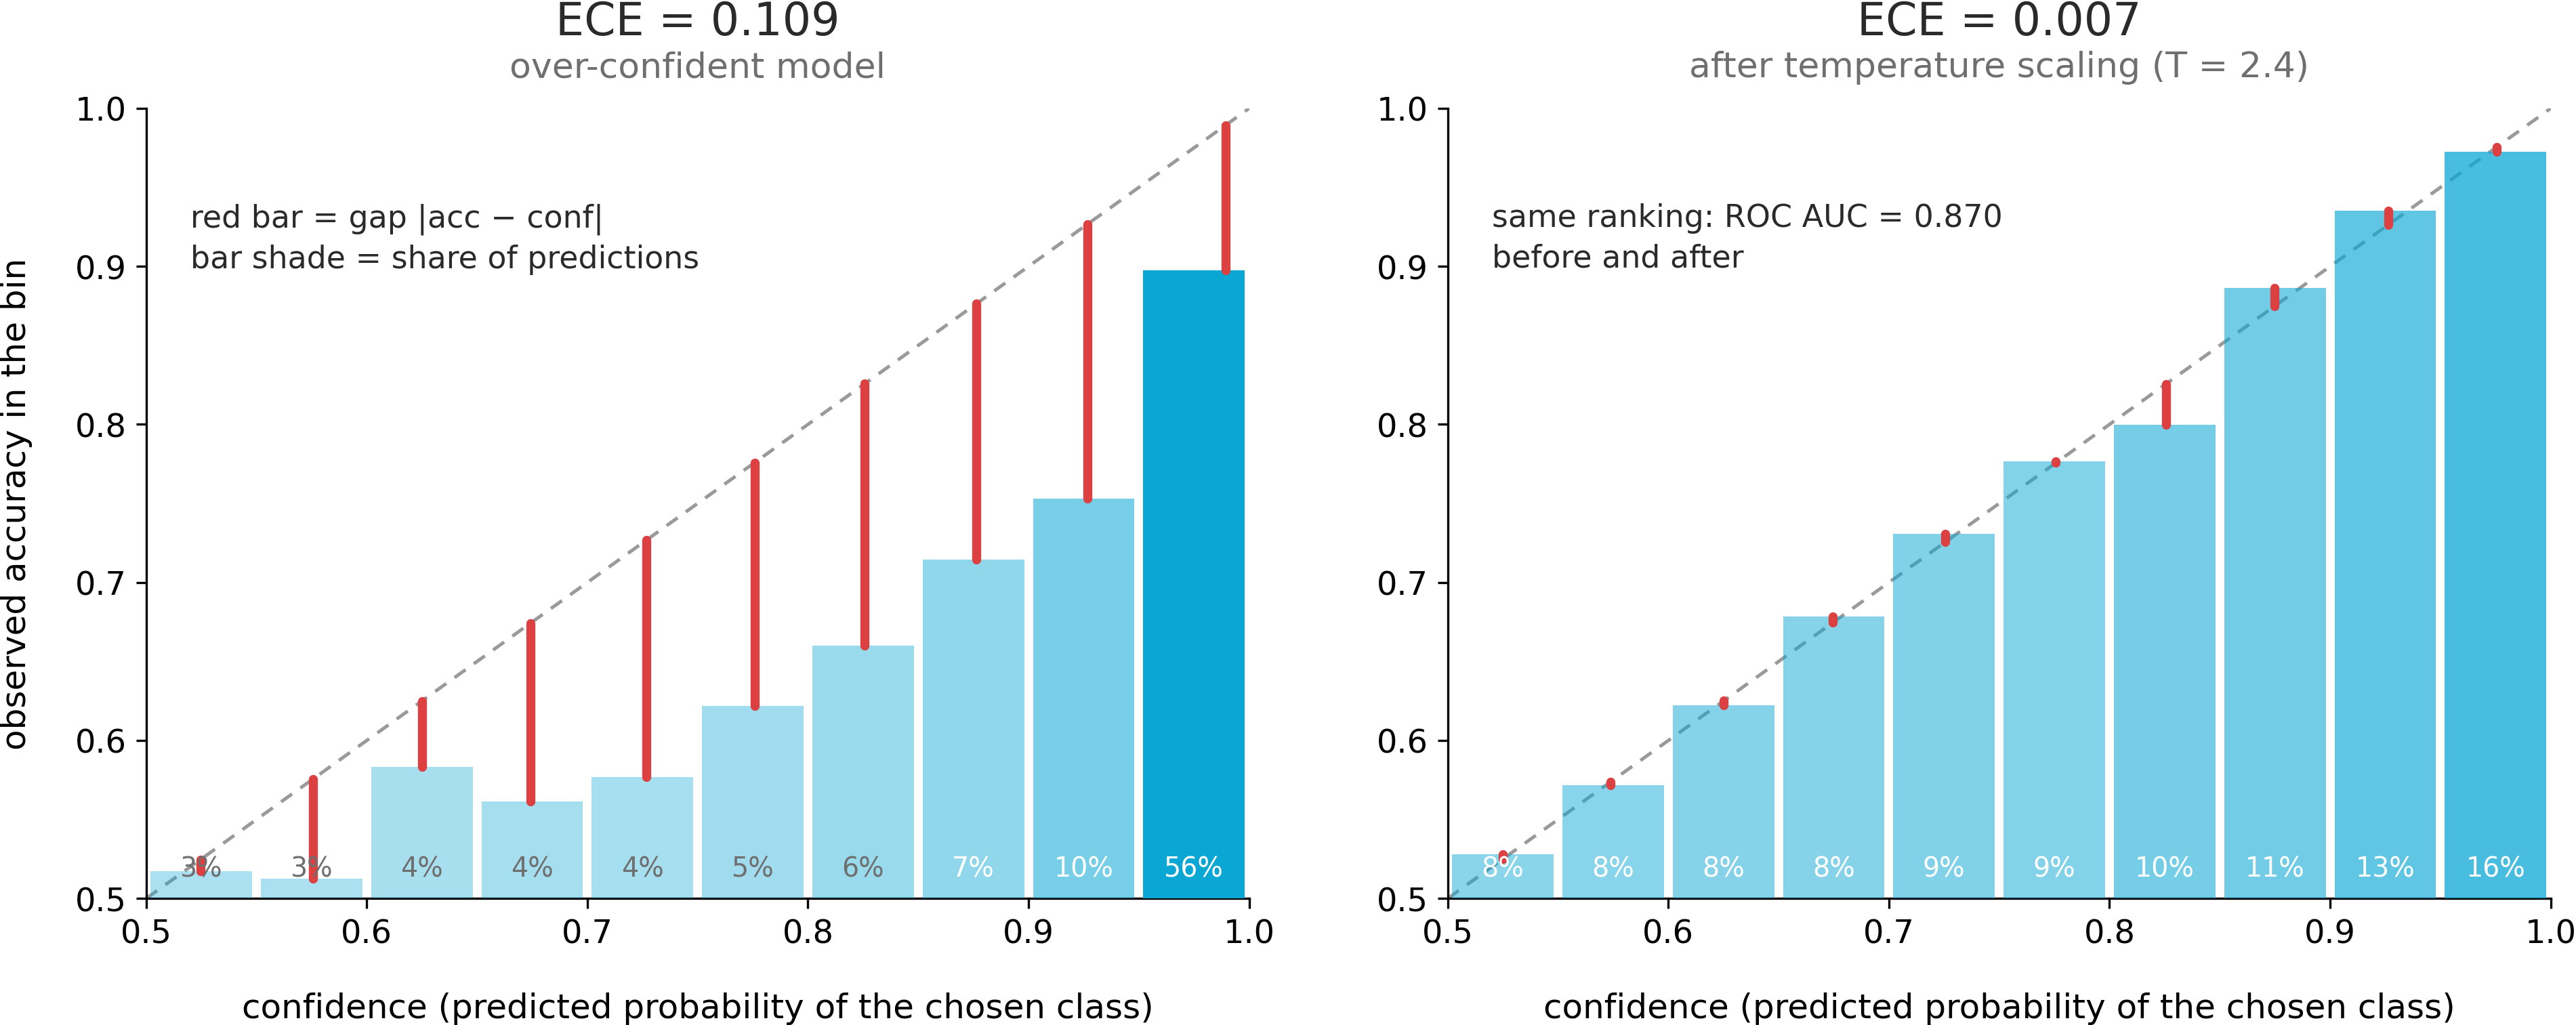
\includegraphics[width=\textwidth]{figures/ECE_reliability.png}
\end{center}

\textbf{Figure. ECE.} Reliability diagrams for a simulated binary classifier before and after temperature scaling, which adjusts
confidence by dividing the model's raw scores (logits) by a positive value $T$. Each bar is a confidence bin: its
height is the observed accuracy, its shade the share of predictions, and the red segment the gap to the diagonal.
\underline{Left:} the model puts $55\%$ of its predictions in the top bin at a mean confidence of $0.99$ and is right $90\%$ of
the time there; the weighted gaps sum to $\text{ECE} = 0.110$. \underline{Right:} with $T = 2.5$, the bars move closer to the
diagonal and ECE falls to $0.007$. ROC AUC stays at $0.867$ because the ranking is unchanged in this binary example.

\orangebox{Did you know that...}
{DeGroot and Fienberg ($1983$) separated the Brier score into calibration and refinement terms. Calibration describes whether
probabilities match outcome frequencies; refinement describes how well the forecasts separate cases with different outcome rates.
A model that gives everyone the overall event rate can be calibrated while offering no such separation. Temperature scaling
illustrates another distinction: it preserves the predicted class in both binary and multiclass classification, but only in the
binary case does it necessarily preserve the ranking of probabilities across examples, and hence ROC AUC.}

\textbf{Other related metrics}

Brier score and log loss evaluate the probabilities as a whole, while ROC AUC measures ranking. Log loss can improve without
changing either ROC AUC or binned ECE, so read them together before explaining a change. Calibration within Groups
(Bias \& Fairness chapter) can reveal errors hidden by pooling groups; CBPE additionally needs calibration to hold in production.

% ---------- CBPE ----------
\clearpage
\thispagestyle{probabilisticstyle}
\section{CBPE}\label{sec:cbpe}
\subsection{Confidence-Based Performance Estimation}

% reference:
% https://nannyml.readthedocs.io/en/stable/how_it_works/performance_estimation.html#confidence-based-performance-estimation-cbpe
% https://arxiv.org/abs/2505.05295 (Kivimäki, Białek, Kuberski, Nurminen, 2025)

CBPE estimates a classifier's performance from probabilities before labels arrive. A fraud model can therefore be monitored
while chargebacks are still pending. Here, $c_j$ is the calibrated probability of fraud and $\hat{y}_j$ the predicted label.
A transaction flagged as fraud with $c_j=0.9$ contributes $0.9$ to expected
true positives and $0.1$ to expected false positives.

% equation
\begin{center}
    \tikz{
        \node[inner sep=2pt, font=\Large] (a) {
            {
                $\displaystyle
                \widehat{\text{TP}} = \sum_{j} {\color{nmlpurple}c_j}\, \mathds{1}[{\color{nmlpurple}\hat{y}_j} = 1], \qquad
                \widehat{\text{FP}} = \sum_{j} (1 - {\color{nmlpurple}c_j})\, \mathds{1}[{\color{nmlpurple}\hat{y}_j} = 1]
                $
            }
        };
        \node[below=0.12cm of a, inner sep=2pt, font=\large] (b) {
            $\displaystyle
            \widehat{\text{FN}} = \sum_{j} {\color{nmlpurple}c_j}\, \mathds{1}[{\color{nmlpurple}\hat{y}_j} = 0], \qquad
            \widehat{\text{TN}} = \sum_{j} (1 - {\color{nmlpurple}c_j})\, \mathds{1}[{\color{nmlpurple}\hat{y}_j} = 0]
            $
        };
        \draw[overlay,-latex,nmlpurple, semithick] ($(a.north)+(-2.50,-0.22)$) to node[pos=1, above] {calibrated probability} +(0.00,0.30);
        \draw[overlay,-latex,nmlpurple, semithick] ($(a.north)+(3.27,-0.36)$) to node[pos=1, above] {predicted label} +(0.00,0.43);
    }
\end{center}

The indicator $\mathds{1}$ selects the predictions with the stated label, and each sum runs over one production batch. An
unflagged transaction contributes $c_j$ to expected false negatives and $1-c_j$ to expected true negatives. Substituting these
counts into metric formulas gives expected accuracy and precision, and approximations for recall and F1.

\textbf{When to use CBPE?}

Use CBPE when labels are delayed and calibration is expected to hold in production. Fit the calibrator on labeled reference
predictions and validate the estimates on separate data. If a changing input mix disrupts calibration, consider PAPE; neither
method can reliably estimate performance for inputs absent from the reference data.

\enlargethispage{2\baselineskip}
\coloredboxes{
\item Estimates several metrics from one expected confusion matrix, without waiting for production labels.
\item Can follow performance changes caused by a new input mix when calibration still holds.
}
{
\item Misses concept drift when inputs stay the same: changed outcomes do not change the model's probabilities.
\item Estimated accuracy is at least $0.5$ if each label chooses the more likely class under the probabilities used.
}

\clearpage

\thispagestyle{customstyle}
\enlargethispage{\baselineskip}

\begin{center}
    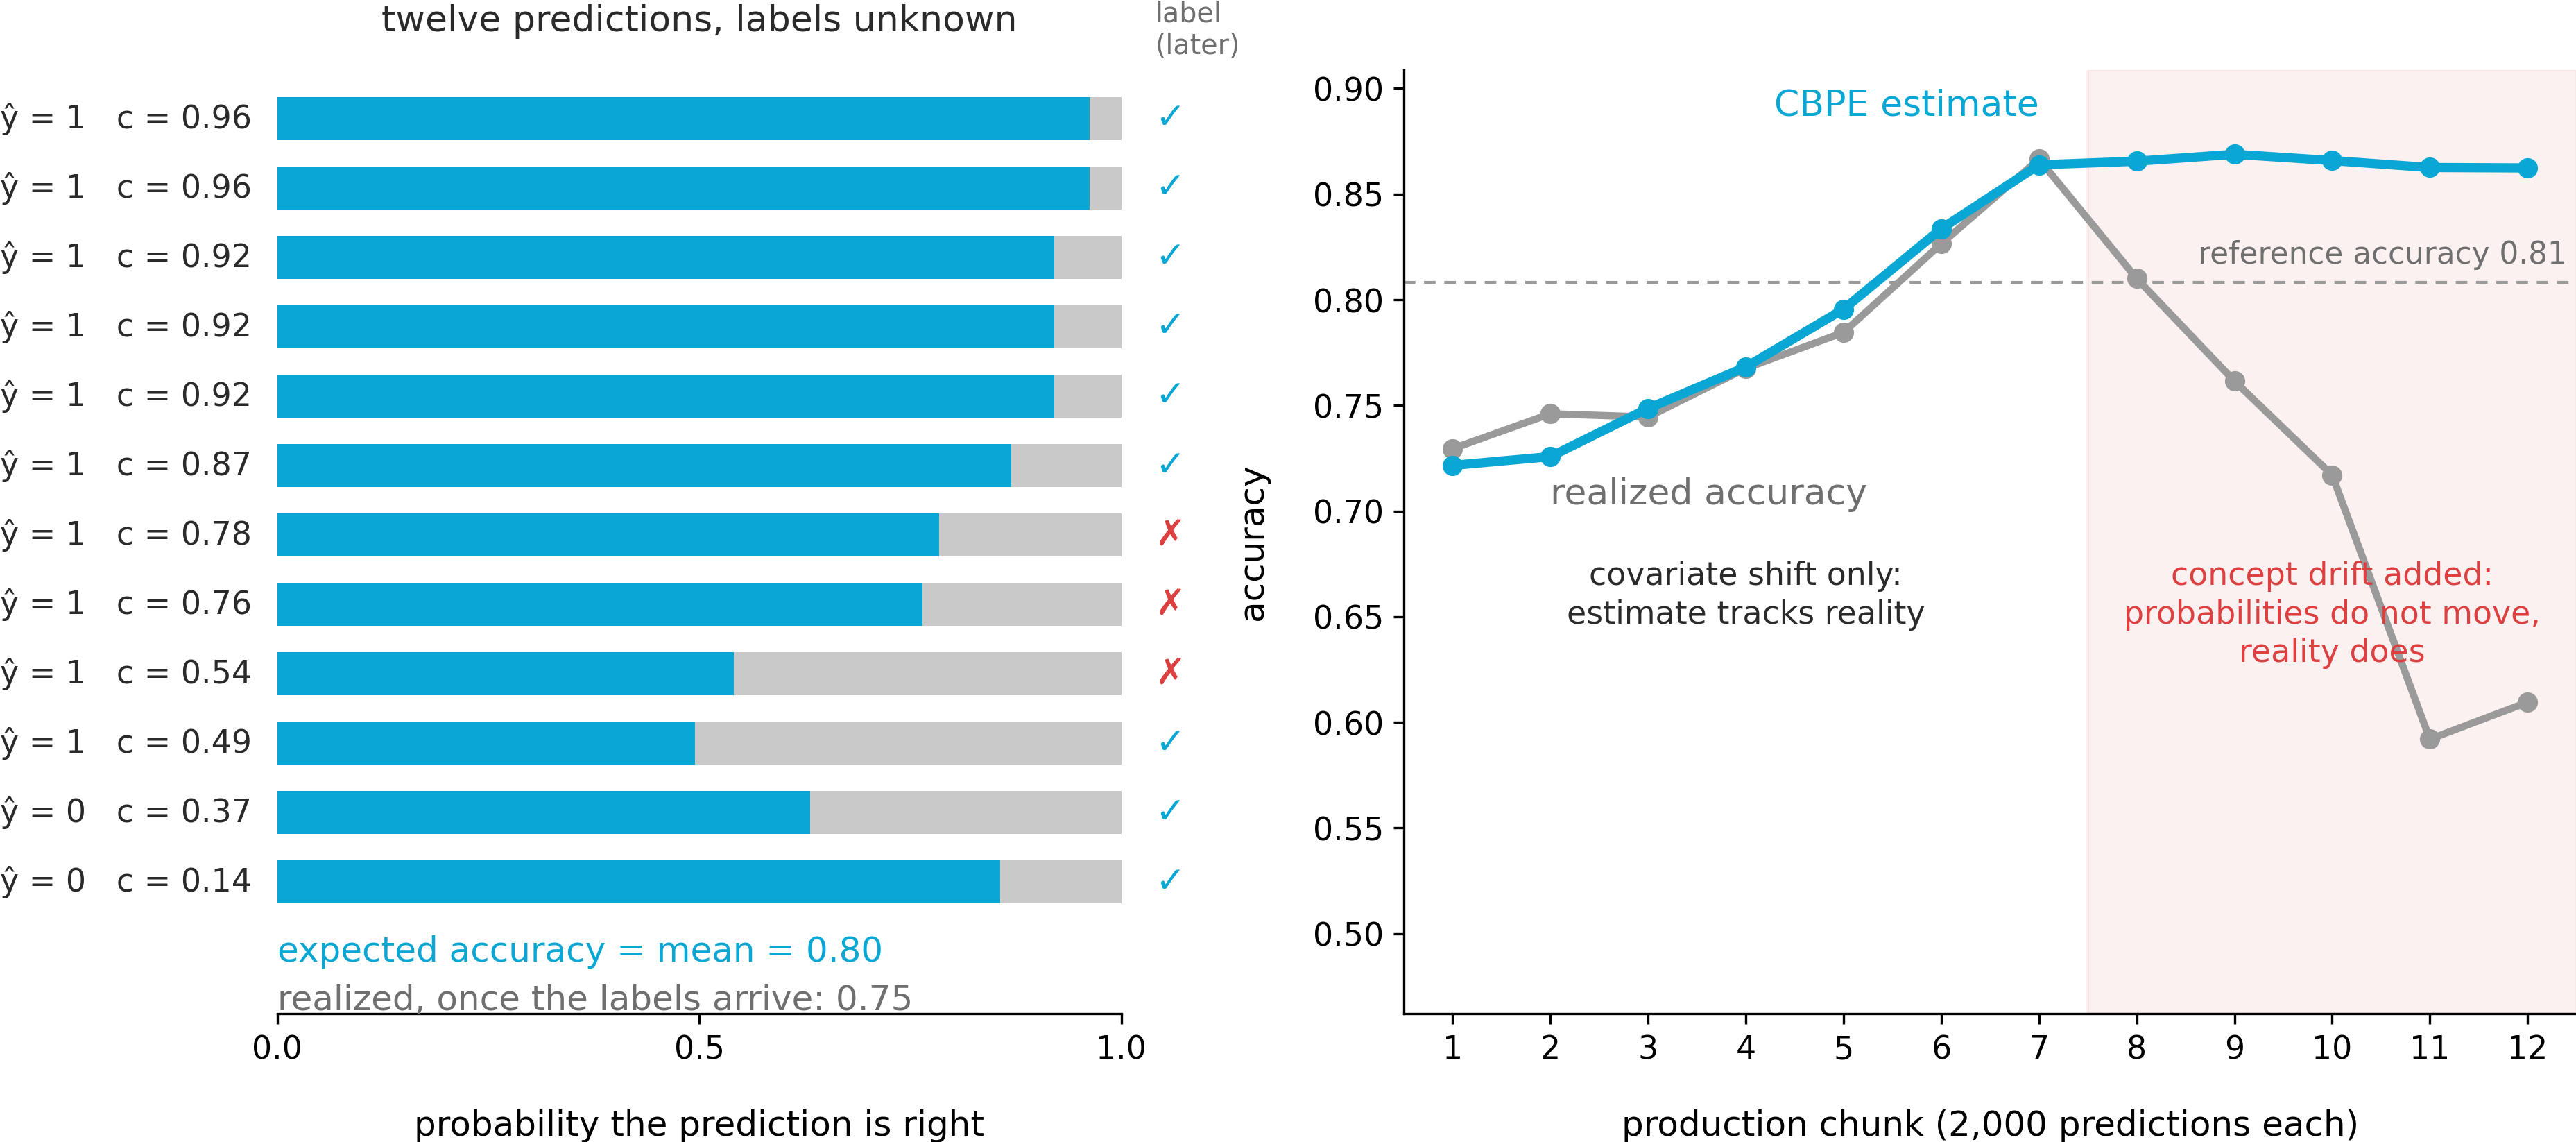
\includegraphics[width=\textwidth]{figures/CBPE_estimation.png}
\end{center}

\textbf{Figure. CBPE.} \underline{Left:} twelve production predictions with calibrated probabilities and no labels. Each bar is the
probability the prediction is right, $c$ for $\hat{y}=1$ and $1-c$ for $\hat{y}=0$; their mean, $0.77$, is the expected accuracy. The
labels that arrive later make nine of twelve right, $0.75$. \underline{Right:} twelve simulated chunks of $2{,}000$ predictions.
Accuracy rises as the input mix changes in chunks $1$--$7$. From chunk $8$, the input--outcome relationship changes too: accuracy
falls to $0.60$, while the estimate stays near $0.86$. The illustrative band follows the estimate at $\pm 3$ standard deviations
of reference-chunk accuracy; it is neither a validated uncertainty interval nor a fixed alert threshold.

\orangebox{Did you know that...}
{Even a sound estimate need not equal the accuracy measured when labels arrive. For $2{,}000$ independent predictions, each with
an $80\%$ chance of being correct, the standard error of accuracy is $\sqrt{0.8(1-0.8)/2{,}000}\approx0.009$, almost one percentage
point. Uncertainty intervals account for variation around an estimate, while historical alert thresholds flag changes from past
performance. To judge a gap, consider both sampling variation and estimation error.}

\textbf{Other related metrics}

Low reference ECE does not bound production error. PAPE adjusts calibration for a changed input mix, but its estimates also need
validation. When labels arrive, investigate gaps between estimated and measured performance; RCD can help assess concept drift,
while estimator error and sampling variation may also contribute.

% ---------- PAPE ----------
\clearpage
\thispagestyle{probabilisticstyle}
\section{PAPE}\label{sec:pape}
\subsection{Probabilistic Adaptive Performance Estimation}

% reference:
% https://docs.nannyml.com/cloud/model-monitoring/how-it-works/probabilistic-adaptive-performance-estimation-pape
% https://arxiv.org/abs/2401.08348 — Estimating Model Performance Under Covariate Shift Without Labels

PAPE estimates classification performance by adapting calibration to the production input mix. Suppose a loan model assigns
$80\%$ repayment probability to two equally sized applicant groups, but their repayment rates are $90\%$ and $70\%$. The combined
rate is $80\%$, so calibration looks right. If the first group becomes more common, the combined rate rises even though neither
group's behavior changed. PAPE gives reference examples from that group more weight when refitting the calibrator.

% equation
\begin{center}
    \tikz{
        \node[inner sep=2pt, font=\Large] (a) {
            {
                $\displaystyle
                \hat{w}(x) = \frac{{\color{nmlred}n_{\text{ref}}}}{{\color{nmlred}n_{\text{prod}}}} \cdot \frac{{\color{nmlpurple}\hat{p}}(z = 1 \mid x)}{{\color{nmlpurple}\hat{p}}(z = 0 \mid x)}
                $
            }
        };
        \path[room for labels] ([yshift=0.13cm]a.north) ([yshift=-0.18cm]a.south);
        \draw[overlay,-latex,nmlred, semithick] ($(a.north)+(-0.60,-0.18)$) to[bend right=15] node[pos=1, left] {sample sizes} +(-1.00,0.30);
        \draw[overlay,-latex,nmlpurple, semithick] ($(a.south)+(0.48,0.09)$) to[bend left=15] node[pos=1, left] {domain classifier} +(-1.00,-0.30);
    }
\end{center}

$\hat{w}(x)$ estimates the density ratio $p_{\text{prod}}(x)/p_{\text{ref}}(x)$ from a classifier trained to tell production
($z=1$) from reference ($z=0$): inputs twice as common get weight $2$. The calibrator is fit on reference labels with these weights,
applied to production scores, and the confusion matrix is built as in CBPE.

\textbf{When to use PAPE?}

Use PAPE when a changed customer mix may have disrupted calibration, provided the reference data covers the inputs seen in
production. Check that enough reference examples support the new mix. Weighting cannot supply missing examples or reveal
concept drift without new labels.

\enlargethispage{\baselineskip}
\coloredboxes{
\item Uses production inputs to adjust reference calibration, so it can follow changes that a fixed calibrator misses.
\item Recomputes weights for each chunk, allowing the calibration adjustment to change as the customer mix changes.
}
{
\item Cannot extrapolate: the density ratio is undefined where production has inputs with no reference support.
\item Inaccurate weights distort calibration. If a few reference examples carry most of the weight, the estimate can be unstable even with many rows.
}

\clearpage

\thispagestyle{customstyle}

\begin{center}
    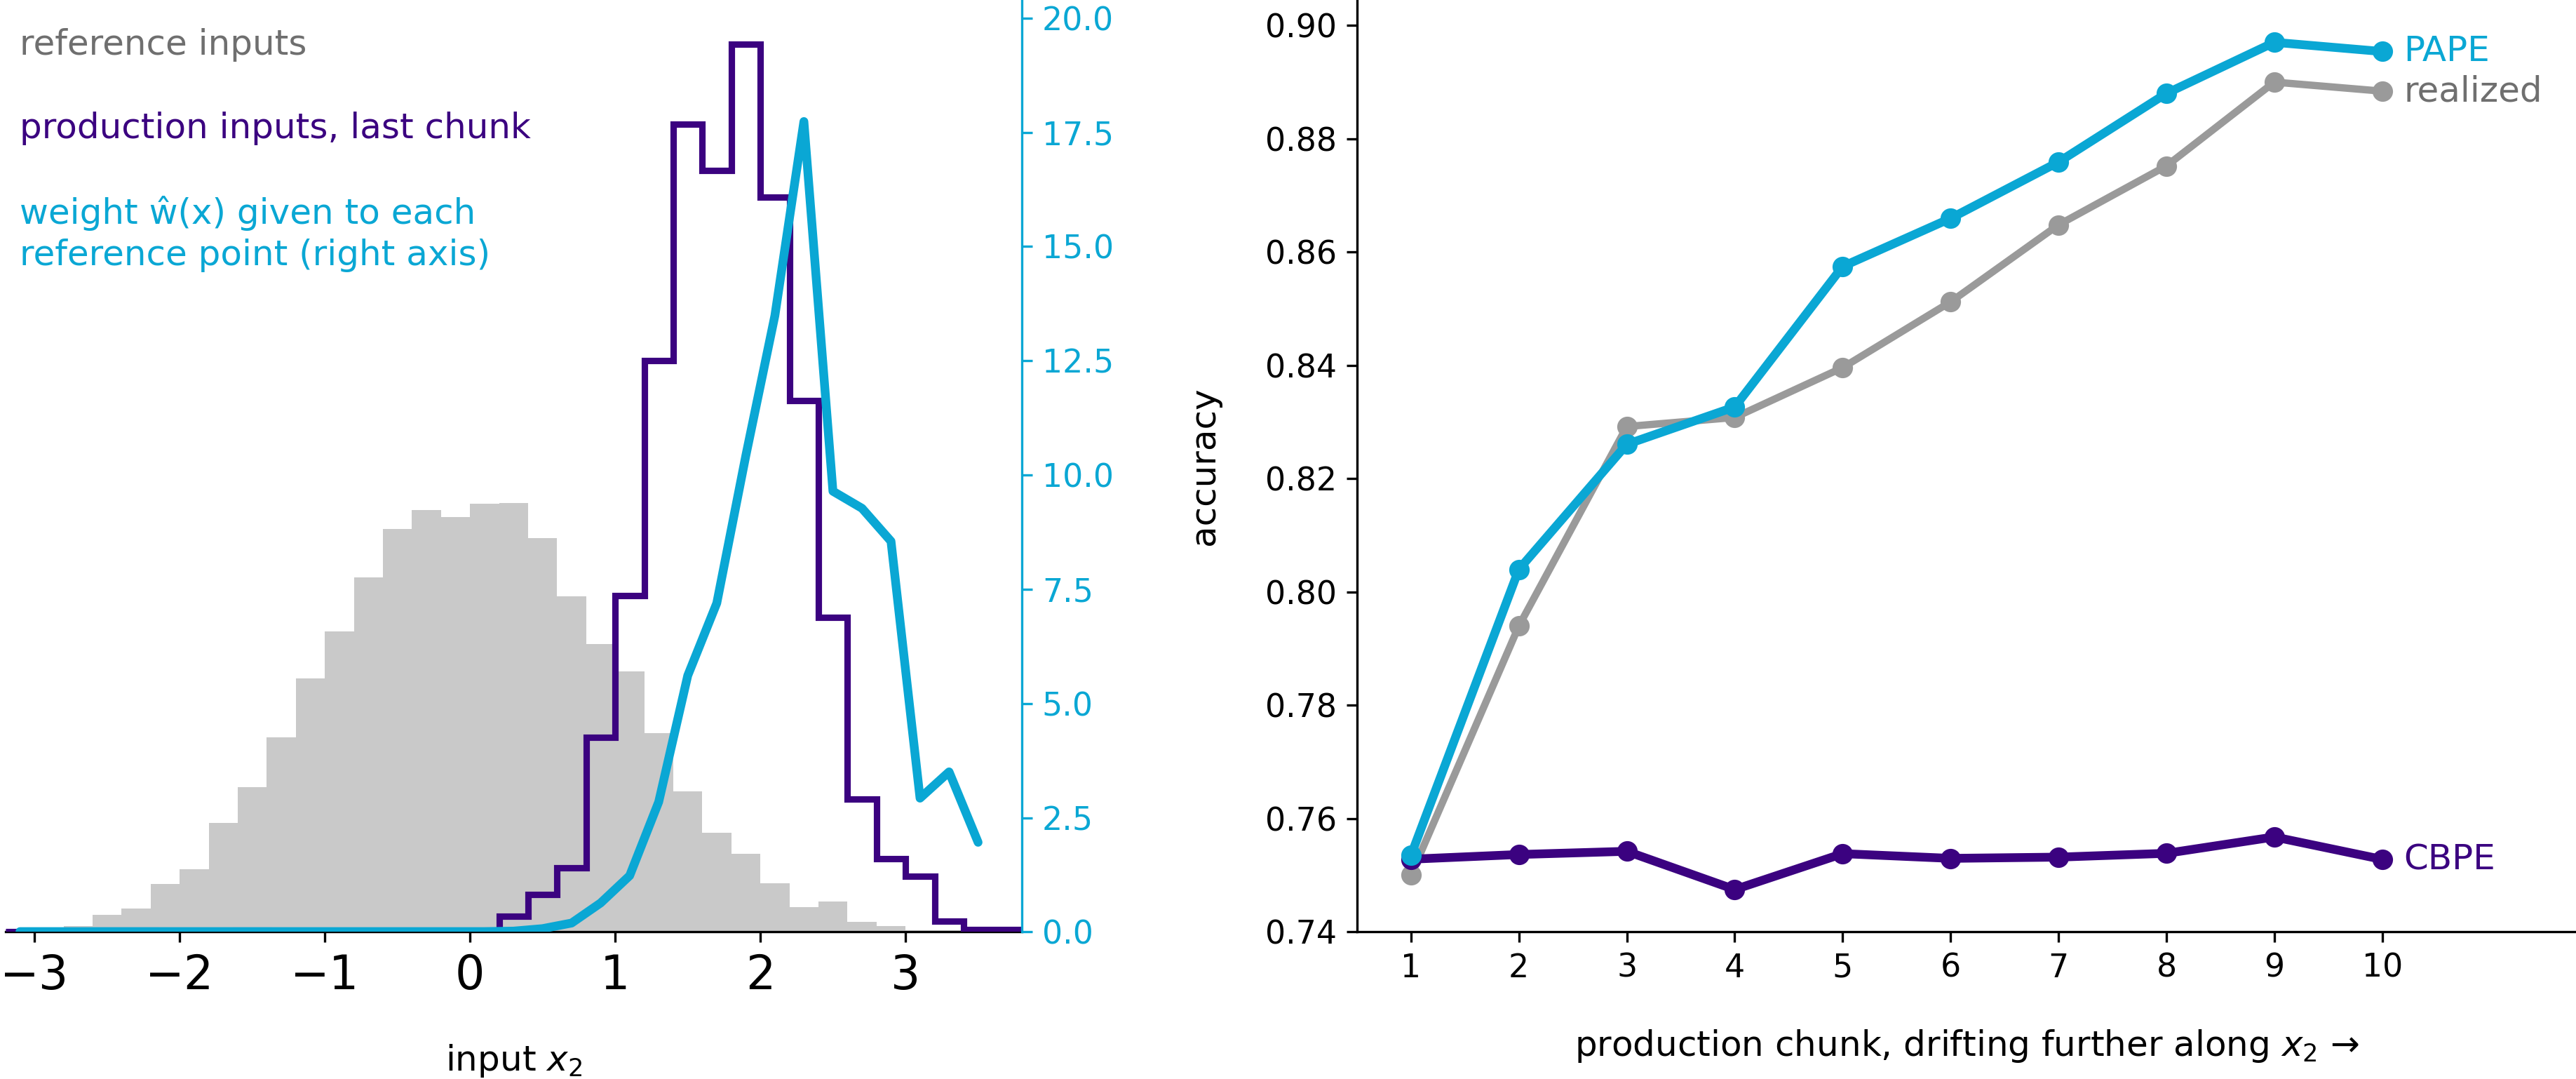
\includegraphics[width=\textwidth]{figures/PAPE_reweighting.png}
\end{center}

\textbf{Figure. PAPE.} A simulated classifier whose calibration varies with an artificial input, $x_2$.
\underline{Left:} the reference (gray) and final production chunk (purple) have different input distributions. The curve shows
the mean weight assigned to reference points at each $x_2$, about $18$ near the production region and close to zero elsewhere.
\underline{Right:} CBPE uses the fixed reference calibration and stays near $0.75$ while realized accuracy climbs to
$0.89$; PAPE follows it with a mean absolute error of $0.009$ against CBPE's $0.089$.

\orangebox{Did you know that...}
{Importance weighting can estimate performance directly by giving more weight to errors on reference examples that resemble
production. PAPE instead uses those weights to fit a calibrator, then estimates performance from production predictions.
In Białek and colleagues' $2025$ benchmark, covering $959$ evaluation cases and $36{,}557$ production chunks from US census data,
PAPE had the lowest aggregate error for accuracy, F1, and ROC AUC among eight evaluated methods. That result supports the approach
in those experiments; it does not guarantee that weighting improves every estimate.}

\textbf{Other related metrics}

If CBPE and PAPE disagree, check whether production inputs are covered by the reference data and whether a few examples dominate
the weights. Compare both estimates with measured performance on labeled periods with similar shifts before choosing between them.
DLE estimates regression loss; RCD uses new labels to assess the effect of a changed input--outcome relationship.

% ---------- DLE ----------
\clearpage
\thispagestyle{probabilisticstyle}
\section{DLE}\label{sec:dle}
\subsection{Direct Loss Estimation}

% reference:
% https://nannyml.readthedocs.io/en/stable/how_it_works/performance_estimation.html#direct-loss-estimation-dle

Direct Loss Estimation estimates a regression model's performance by learning how large its errors tend to be for different
inputs. A demand forecast, for example, may be more accurate for staples than for promotions. DLE trains a second model on
reference errors, then averages its predicted losses over each production batch. In NannyML's terminology, this loss model is
the \emph{nanny}, and the monitored model is the \emph{child}.

% equation
\begin{center}
    \tikz{
        \node[inner sep=2pt, font=\Large] (a) {
            {
                $\displaystyle
                \widehat{\text{MAE}} = \frac{1}{{\color{nmlred}n}} \sum_{j=1}^{n} {\color{nmlpurple}h}\big({\color{nmlcyan}x_j},\, {\color{nmlpurple}f(x_j)}\big)
                $
            }
        };
        \path[room for labels] ([yshift=0.19cm]a.north) ([yshift=-0.00cm]a.south);
        \draw[overlay,-latex,nmlred, semithick] ($(a.south)+(-0.93,0.42)$) to[bend left=15] node[pos=1, left] {production size} +(-1.00,-0.30);
        \draw[overlay,-latex,nmlpurple, semithick] ($(a.north)+(0.28,-0.52)$) to[bend right=15] node[pos=1, left] {nanny model} +(-1.00,0.72);
        \draw[overlay,-latex,nmlcyan, semithick] ($(a.south)+(1.05,0.63)$) to[bend right=15] node[pos=1, right] {input} +(1.00,-0.30);
        \draw[overlay,-latex,nmlpurple, semithick] ($(a.north)+(2.45,-0.51)$) to node[pos=1, above] {child's prediction} +(0.00,0.33);
    }
\end{center}

For MAE, train $h$ to predict $|y-f(x)|$ from the inputs and the monitored model's prediction $f(x)$. These errors must come from
data that $f$ did not train on. For MSE, predict squared errors instead; for RMSE, take the square root after averaging them.
Validate $h$'s estimates on separate labeled data before using them for monitoring.

\textbf{When to use DLE?}

Use DLE when regression targets arrive late and the input mix changes. It is useful when expected loss varies predictably across
inputs, whether because of noise or systematic model errors. It cannot reliably handle a changed input--outcome relationship
or inputs outside the reference data.

\enlargethispage{\baselineskip}
\coloredboxes{
\item Estimates familiar regression metrics directly from losses, without having to model the full distribution of possible outcomes.
\item Error size can be easier to predict than the outcome itself: a promotion may have uncertain demand but consistently larger errors.
}
{
\item Assumes learned error patterns still hold. If errors grow for unchanged inputs, the loss model continues to predict the earlier error.
\item A second model needs training and validation. Noisy reference losses or a poorly fitted loss model can distort the performance estimate.
}

\clearpage

\thispagestyle{customstyle}

\begin{center}
    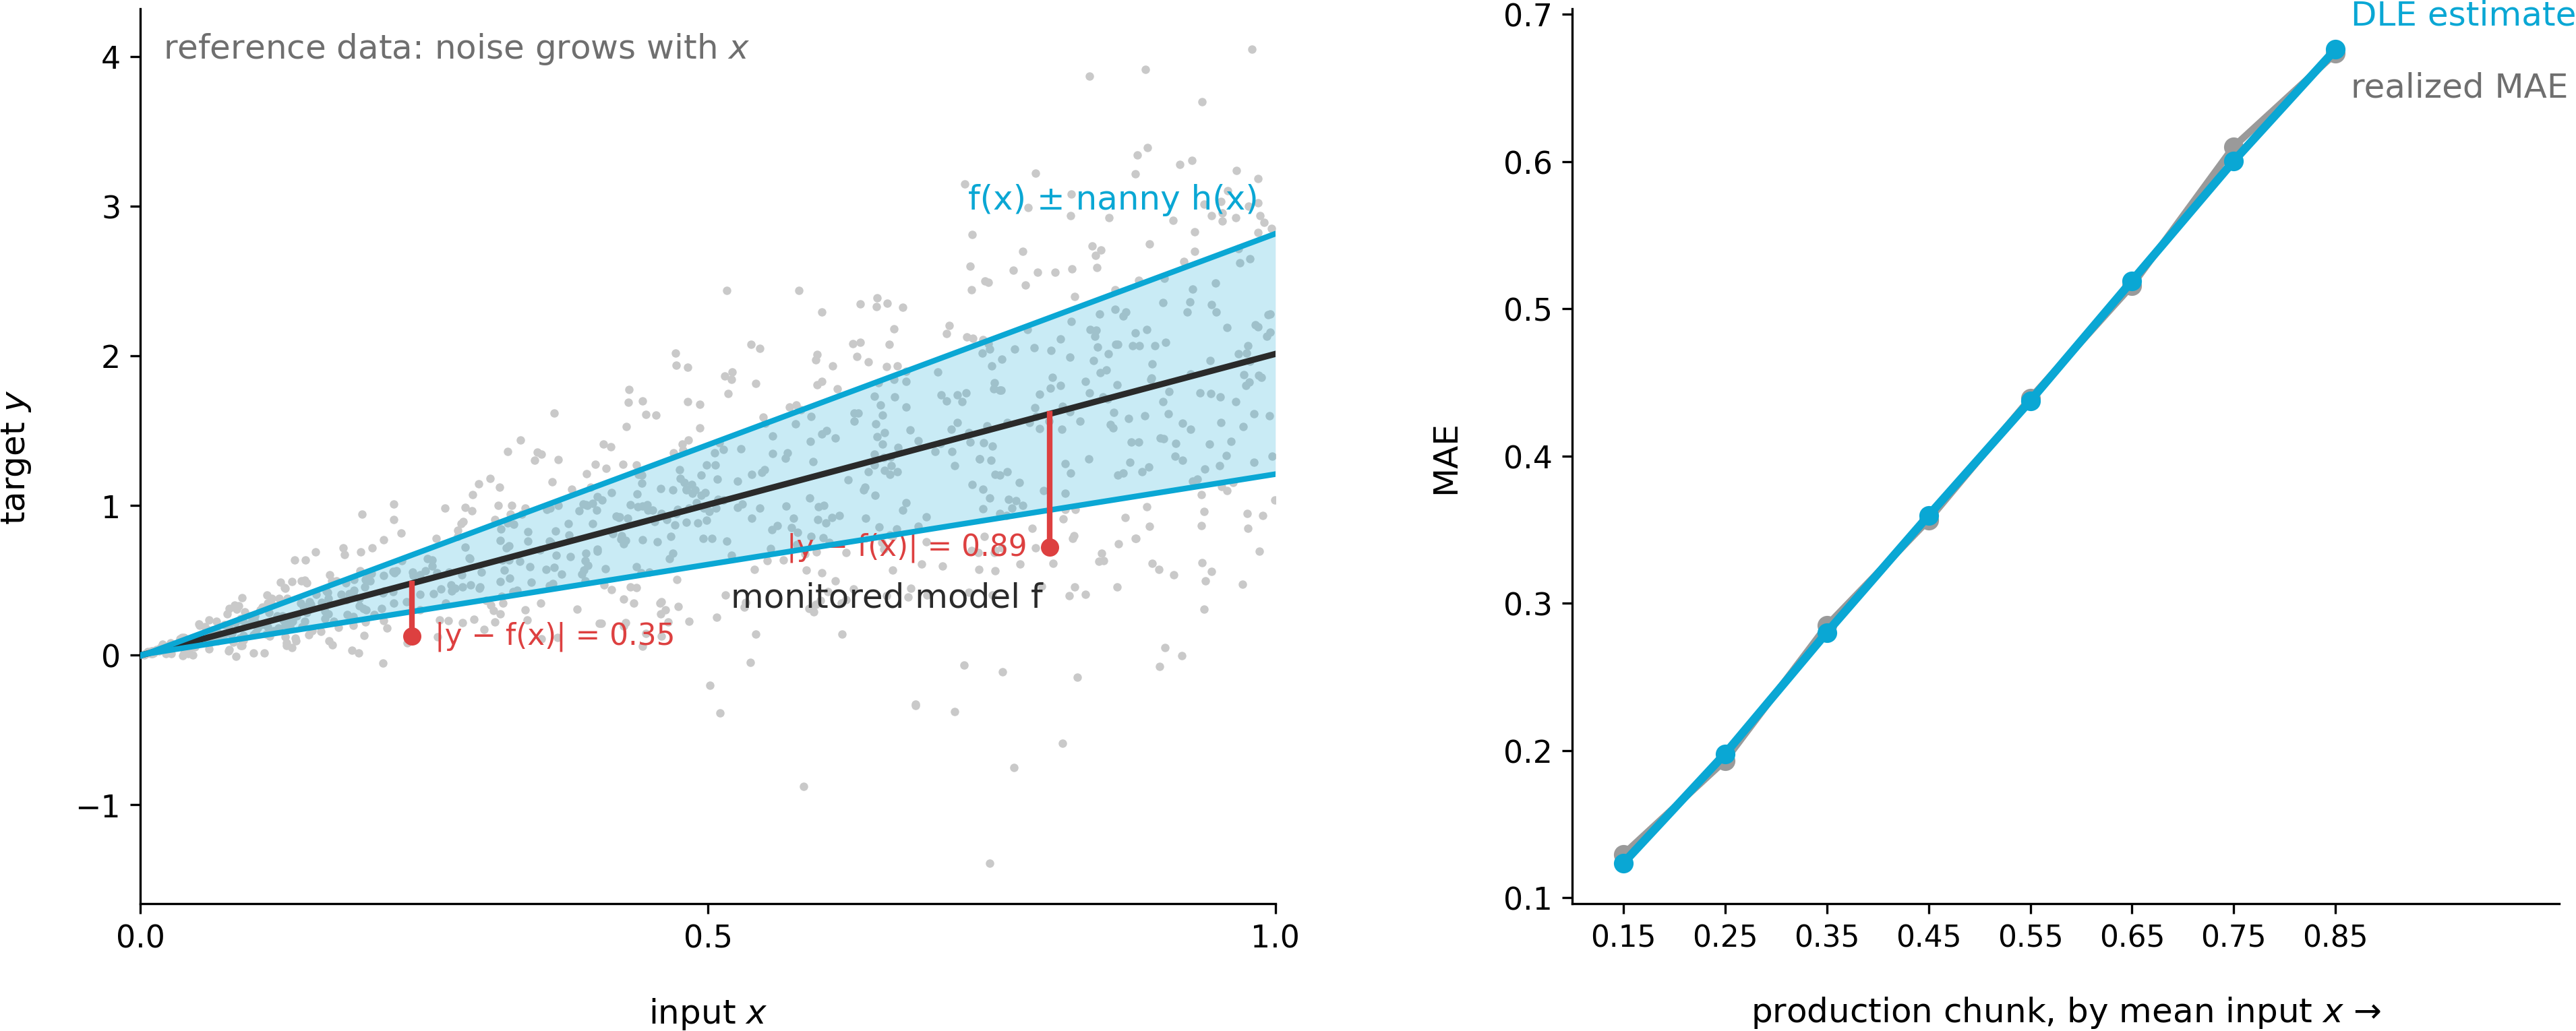
\includegraphics[width=\textwidth]{figures/DLE_nanny.png}
\end{center}

\textbf{Figure. DLE.} \underline{Left:} simulated data whose noise grows with the input, a linear prediction model $f$, and a
linear loss model $h$. The shaded band shows $f(x)\pm h(x)$: the prediction plus or minus the estimated mean absolute error.
It illustrates error size, with no stated coverage probability. Two absolute errors used to train $h$ are marked in red.
\underline{Right:} eight production chunks move toward the noisier region. Measured MAE rises from $0.13$ to $0.67$, and DLE
tracks it to within $0.01$ in this example.

\orangebox{Did you know that...}
{NannyML explored Bayesian models and conformalized quantile regression before adopting DLE. One attempt converted two predicted
quantiles into an outcome distribution by assuming it was normal, then calculated expected loss from that distribution.
Predicting the loss directly removed those intermediate steps. The normality assumption belonged to that particular conversion:
conformal prediction itself does not require normally distributed noise. Its usual coverage guarantee instead depends on
calibration and future examples being exchangeable, as they are under independent sampling from the same distribution.}

\textbf{Other related metrics}

CBPE and PAPE estimate classification performance; DLE learns the loss directly. When measured and estimated loss disagree,
check input changes, recent labeled errors, and the loss model's validation results. The gap may reflect concept drift, poor
estimation, or sampling variation, and input monitoring alone cannot distinguish them.

% ---------- RCD ----------
\clearpage
\thispagestyle{probabilisticstyle}
\section{RCD}\label{sec:rcd}
\subsection{Reverse Concept Drift}

% reference:
% https://docs.nannyml.com/cloud/model-monitoring/how-it-works/reverse-concept-drift-rcd

Reverse Concept Drift estimates how a changed relationship between inputs and outcomes affects model performance on the
reference population. For a loan model, it keeps the earlier applicants' inputs fixed and estimates how accurate the same model
would be under today's repayment behavior. A separate model $g$ learns that behavior, called the new \emph{concept}, from
recent labeled data.

% equation
\begin{center}
    \tikz{
        \node[inner sep=2pt, font=\Large] (a) {
            {
                $\displaystyle
                \Delta = \underset{x \in \text{ref}}{\text{mean}}\; \mathbb{E}_{\,y \sim {\color{nmlpurple}g}(x)}\Big[\, m(\hat{y}(x),\, y) \Big] - {\color{nmlcyan}m_{\text{ref}}}
                $
            }
        };
        \node[below=0.1cm of a, inner sep=2pt, font=\normalsize] (b) {
            $\mathbb{E}_{\,y \sim {\color{nmlpurple}g}(x)}[m(\hat{y}, y)] = {\color{nmlpurple}g}(x)\, m(\hat{y}, 1) + \big(1 - {\color{nmlpurple}g}(x)\big)\, m(\hat{y}, 0)$
        };
        \draw[overlay,-latex,nmlpurple, semithick] ($(b.south)+(-0.55,0.1)$) to[bend left=15] node[pos=1, left] {new concept} +(-0.5,-.45);
        \draw[overlay,-latex,nmlcyan, semithick] ($(a.north)+(2.9,-0.3)$) to[bend left=15] node[pos=1, right] {reference performance} +(0.2,.5);
    }
\end{center}

The equation shows binary accuracy: $g(x)$ is the estimated probability of class $1$ under the new concept, $m(\hat{y},y)$ is
$1$ for a correct prediction and $0$ otherwise, and $m_{\text{ref}}$ is measured reference accuracy. Averaging over the same
reference inputs holds their mix fixed, so $\Delta$ estimates the accuracy change due to the new concept. F1 and ROC AUC need
different metric calculations.

\textbf{When to use RCD?}

Use RCD after labels arrive to investigate whether changed outcomes for comparable inputs could explain a performance change.
A negative accuracy impact is a reason to evaluate retraining, not a guarantee it will help. Recent labeled data must be sufficient
to learn the new concept across the reference inputs.

\enlargethispage{2\baselineskip}
\coloredboxes{
\item Evaluates a changed concept on a fixed population, avoiding confusion with changes in how common different inputs are.
\item Uses the metric's own units: an accuracy impact of $-0.04$ estimates a four-percentage-point drop on the reference population.
}
{
\item Errors in $g$ can look like concept drift. Check its predictions and calibration on held-out recent data before interpreting the impact.
\item Describes the reference population; it does not capture drift confined to inputs absent from that population.
}

\clearpage

\thispagestyle{customstyle}

\begin{center}
    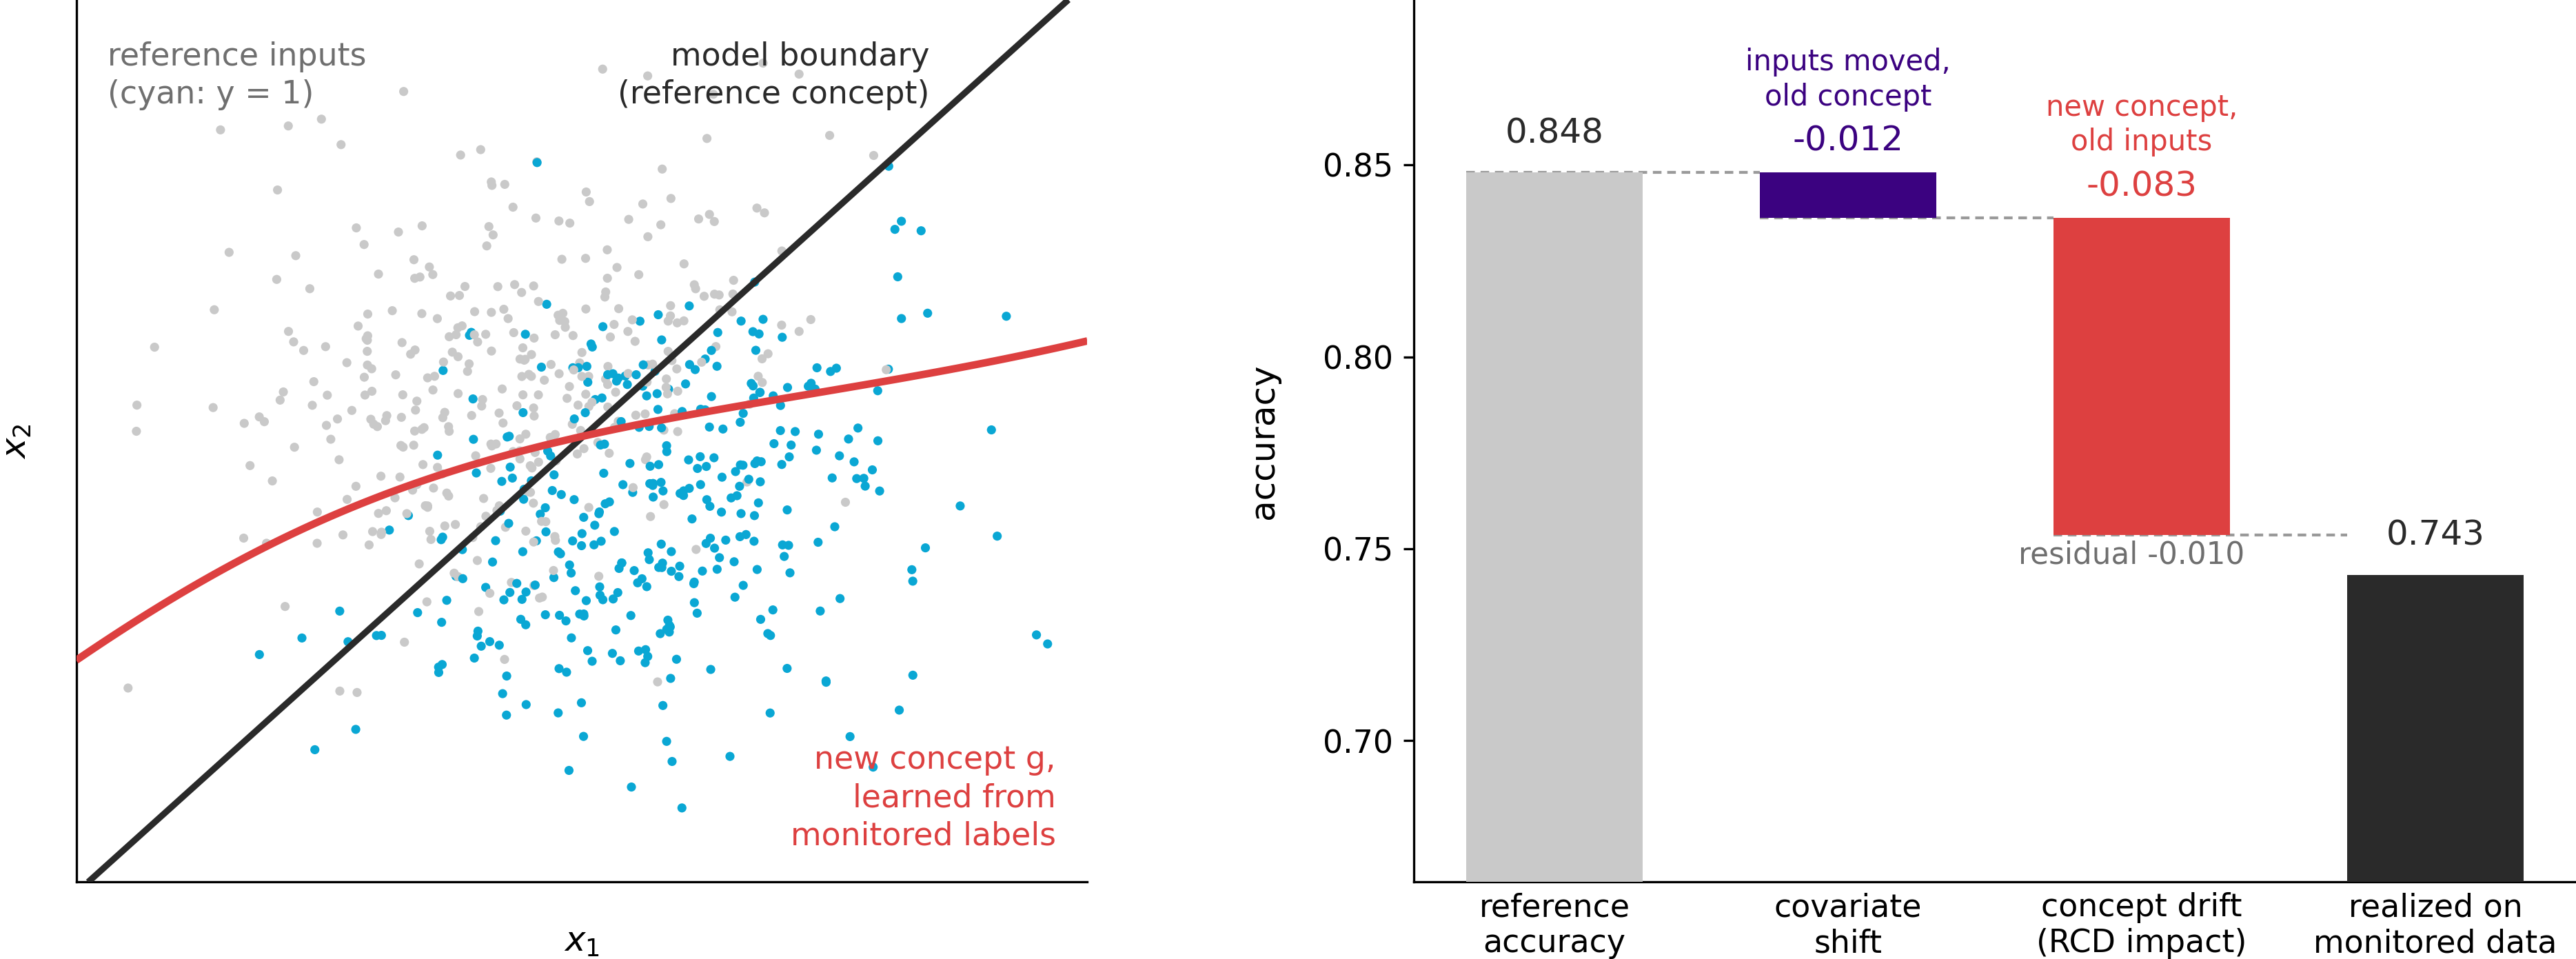
\includegraphics[width=\textwidth]{figures/RCD_decomposition.png}
\end{center}

\textbf{Figure. RCD.} \underline{Left:} simulated reference inputs, the monitored model's decision boundary (black), and the new
concept model's boundary (red). Between them, the models predict different classes. \underline{Right:} measured accuracy falls
from $0.832$ to $0.746$. Changing the input mix while keeping the old concept gives an estimated effect of $+0.010$; applying
the new concept to the reference inputs gives $-0.065$. These reach $0.777$, leaving a residual of $-0.031$. Interaction between
the shifts, concept-model error, and sampling variation can all contribute to that remainder.

\orangebox{Did you know that...}
{A large concept change can leave overall accuracy unchanged. Suppose a model predicts repayment for everyone in two equally
sized groups. Both groups initially repay $80\%$ of the time; later, one repays $100\%$ and the other $60\%$. Each rate changed
by twenty percentage points, but average accuracy is still $80\%$: the improvement in one group cancels the deterioration in
the other. A small overall impact can therefore hide a substantial change for particular groups.}

\textbf{Other related metrics}

CBPE, PAPE, and DLE assume the input--outcome relationship is stable; RCD helps investigate that assumption once labels arrive.
RCD also reports a \emph{magnitude}, $\frac{1}{n}\sum_j |g(x_j)-g_{\text{ref}}(x_j)|$, where $g_{\text{ref}}$ models the old concept
and the sum covers the reference inputs. This measures how much estimated probabilities changed, regardless of their effect on
accuracy. If magnitude is large but impact is small, examine individual groups for changes that cancel in the average.

\include{10-bias-fairness}
\chapteropener{Data Observability}{minthard}{mintaccent}{%
Data observability monitors help check whether data arrives on time and whether its structure and values meet expectations. This chapter covers row counts, timestamps, schema changes, missing and repeated values, and summaries of numeric and text columns.

The figures follow one simulated orders table over six weeks. Rows arriving on the same day form a daily partition. Most monitors compare each day's measurement with a range learned from earlier days; schema monitoring compares column names and types directly. Gray bands show expected ranges, red points mark alerts, and hollow points indicate skipped or unavailable measurements. Each page explains one monitor, what it can detect, and what it can miss.}{In this chapter}

% ---------- Decision map ----------
\begin{decisionmap}{minthard}{mintaccent}{Which monitor?}{Follow the branches to a monitor. The number next to it is its page.}
\maproot{What could have gone wrong upstream?}
\begin{forest} dmap
[, coordinate, l sep=0pt
  [{\dl{you first want to know how any monitor decides}{\mref{Expected Range}{sec:expected-range}}}]
  [{\dm{the data is late or partial}{What do you check?}}
    [{\dl{when it last landed}{\mref{Freshness}{sec:freshness}}}]
    [{\dl{how many rows came}{\mref{Row Count}{sec:row-count}}}]
  ]
  [{\dl{the structure changed}{\mref{Schema Changes}{sec:schema-changes}}}]
  [{\dm{values are missing or repeated}{Which?}}
    [{\dl{empty cells}{\mref{Missing Values}{sec:missing-values}}}]
    [{\dl{rows that should be unique}{\mref{Duplicates}{sec:duplicates}}}]
    [{\dl{the number of distinct values}{\mref{Unique Count}{sec:unique-count}}}]
  ]
  [{\dm{numbers drifted or spiked}{Which part of the distribution?}}
    [{\dl{the center}{\mref{Average}{sec:average}}}]
    [{\dl{the total}{\mref{Sum}{sec:sum}}}]
    [{\dl{the spread}{\mref{Standard Deviation}{sec:standard-deviation}}}]
    [{\dl{the extremes}{\mref{Min and Max}{sec:min-and-max}}}]
    [{\dl{the shape}{\mref{Quartiles}{sec:quartiles}}}]
  ]
  [{\dl{text changed shape}{\mref{Text Length}{sec:text-length}}}]
]
\end{forest}
\mapnotes{Check freshness and row count alongside value monitors: incomplete loads can affect their results. Compare schema changes with the previous or approved schema.}
\end{decisionmap}

% All figures in this chapter come from one simulated `orders` table, monitored daily for 42 days
% (notebooks/observability_plots.py). Metric definitions follow the Soda documentation:
% https://docs.soda.io/data-observability/metric-monitoring-dashboard

% Wording review references:
% https://www.itl.nist.gov/div898/handbook/pmc/section3/pmc31.htm
% https://www.postgresql.org/docs/current/functions-aggregate.html
% https://numpy.org/doc/stable/reference/generated/numpy.quantile.html
% Duplicate percentage counts all non-null rows in repeated-key groups here.
% Tool conventions differ; the expected-range detector is illustrative.

% ---------- Expected Range ----------
\clearpage
\thispagestyle{observabilitystyle}
\section{Expected Range}\label{sec:expected-range}
\subsection{Comparing a Metric with Its History}

An expected range describes the values a monitor considers normal, based on earlier measurements. A value outside this range is flagged for review. In the rule below, $\mu_t$ is the expected value for the day and $\sigma_t$ describes the usual variation around it.

% equation
\begin{center}
    \tikz{
        \node[inner sep=2pt, font=\Large] (a) {
            {
                $\displaystyle
                \text{anomaly at } t \iff \big|\, {\color{nmlcyan}x_t} - {\color{nmlpurple}\mu_t} \,\big| > {\color{nmlyellow}z}\, {\color{nmlpurple}\sigma_t}
                $
            }
        };
        \draw[overlay,-latex,nmlcyan, semithick] ($(a.north)+(0.2,-0.2)$) to[bend right=15] node[pos=1, left] {today's measurement} +(-1,.5);
        \draw[overlay,-latex,nmlpurple, semithick] ($(a.north)+(1.4,-0.2)$) to[bend left=15] node[pos=1, right] {baseline from history} +(0.8,.5);
        \draw[overlay,-latex,nmlyellow, semithick] ($(a.south)+(2.0,0.25)$) to[bend right=15] node[pos=1, left] {sensitivity} +(-0.8,-.5);
        \draw[overlay,-latex,nmlpurple, semithick] ($(a.south)+(2.75,0.25)$) to[bend left=15] node[pos=1, right] {spread of history} +(0.4,-.5);
    }
\end{center}

The setting $z$ controls the width of the range. Lower values flag smaller changes; higher values allow more variation. A common choice for this type of rule is $z=3$, but settings depend on the tool. A good monitor also accepts human feedback: marking an alert as expected can help it learn a legitimate pattern; confirming an incident can help keep bad data out of its baseline.

\begin{center}
    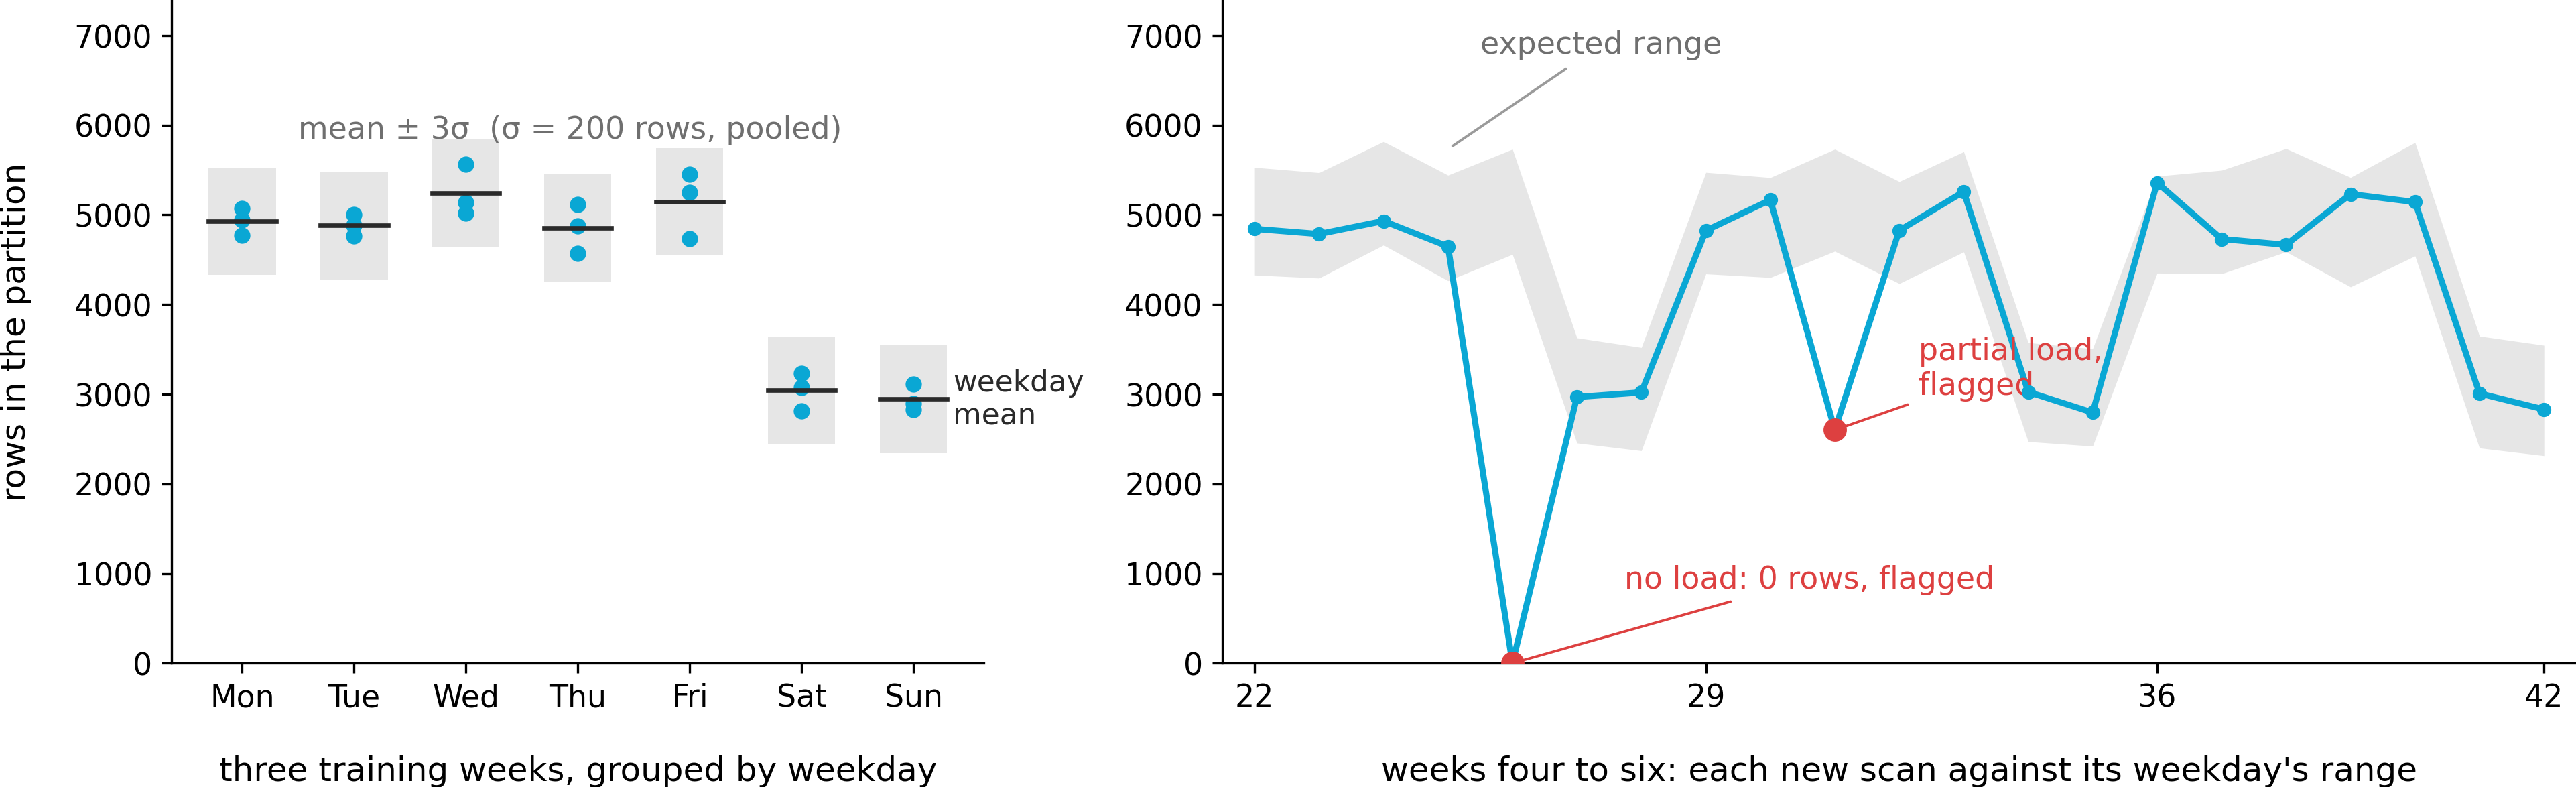
\includegraphics[width=\textwidth]{figures/Observability_expected_range.png}
\end{center}

\textbf{Figure. Expected Range.} Daily counts for a simulated orders table. \underline{Left:} three weeks of data establish an average for each weekday, with a range of about $600$ rows above and below it. \underline{Right:} no load arrives on day $26$, and only part of the load arrives on day $31$. Both counts fall below the range. Lower weekend counts stay within their expected range.

\textbf{When to use it?}

Use a historical range when normal values change over time, for example between weekdays and weekends. Adjust sensitivity to balance missed problems against false alerts. A known requirement, such as zero duplicate keys, is better checked with a fixed limit. A flagged value needs investigation; it is not necessarily an error.

% ---------- Row Count ----------
\clearpage
\thispagestyle{observabilitystyle}
\section{Row Count}\label{sec:row-count}
\subsection{Volume}

Row count tells you how many rows are in a table or a selected part of it. It helps detect missing, incomplete or repeated loads. Here, each scan counts one day's arrivals, called a daily partition.

% equation
\begin{center}
    \tikz{
        \node[inner sep=2pt, font=\Large] (a) {
            {
                $\displaystyle
                \text{rows}_{t} = \sum_{r \in T} \mathds{1}\big[\, {\color{nmlcyan}p(r)} = {\color{nmlpurple}t} \,\big]
                $
            }
        };
        \draw[overlay,-latex,nmlcyan, semithick] ($(a.south)+(0.9,0.3)$) to[bend left=15] node[pos=1, left] {row's partition value} +(-1,-.5);
        \draw[overlay,-latex,nmlpurple, semithick] ($(a.north)+(1.7,-0.2)$) to[bend left=15] node[pos=1, right] {the partition being scanned} +(0.6,.5);
    }
\end{center}

The formula counts rows whose partition date $p(r)$ matches the day $t$ being checked. In SQL, this is \texttt{COUNT(*)} with a date filter. Some databases also provide a row count in their metadata, but it may be approximate or out of date.

\begin{center}
    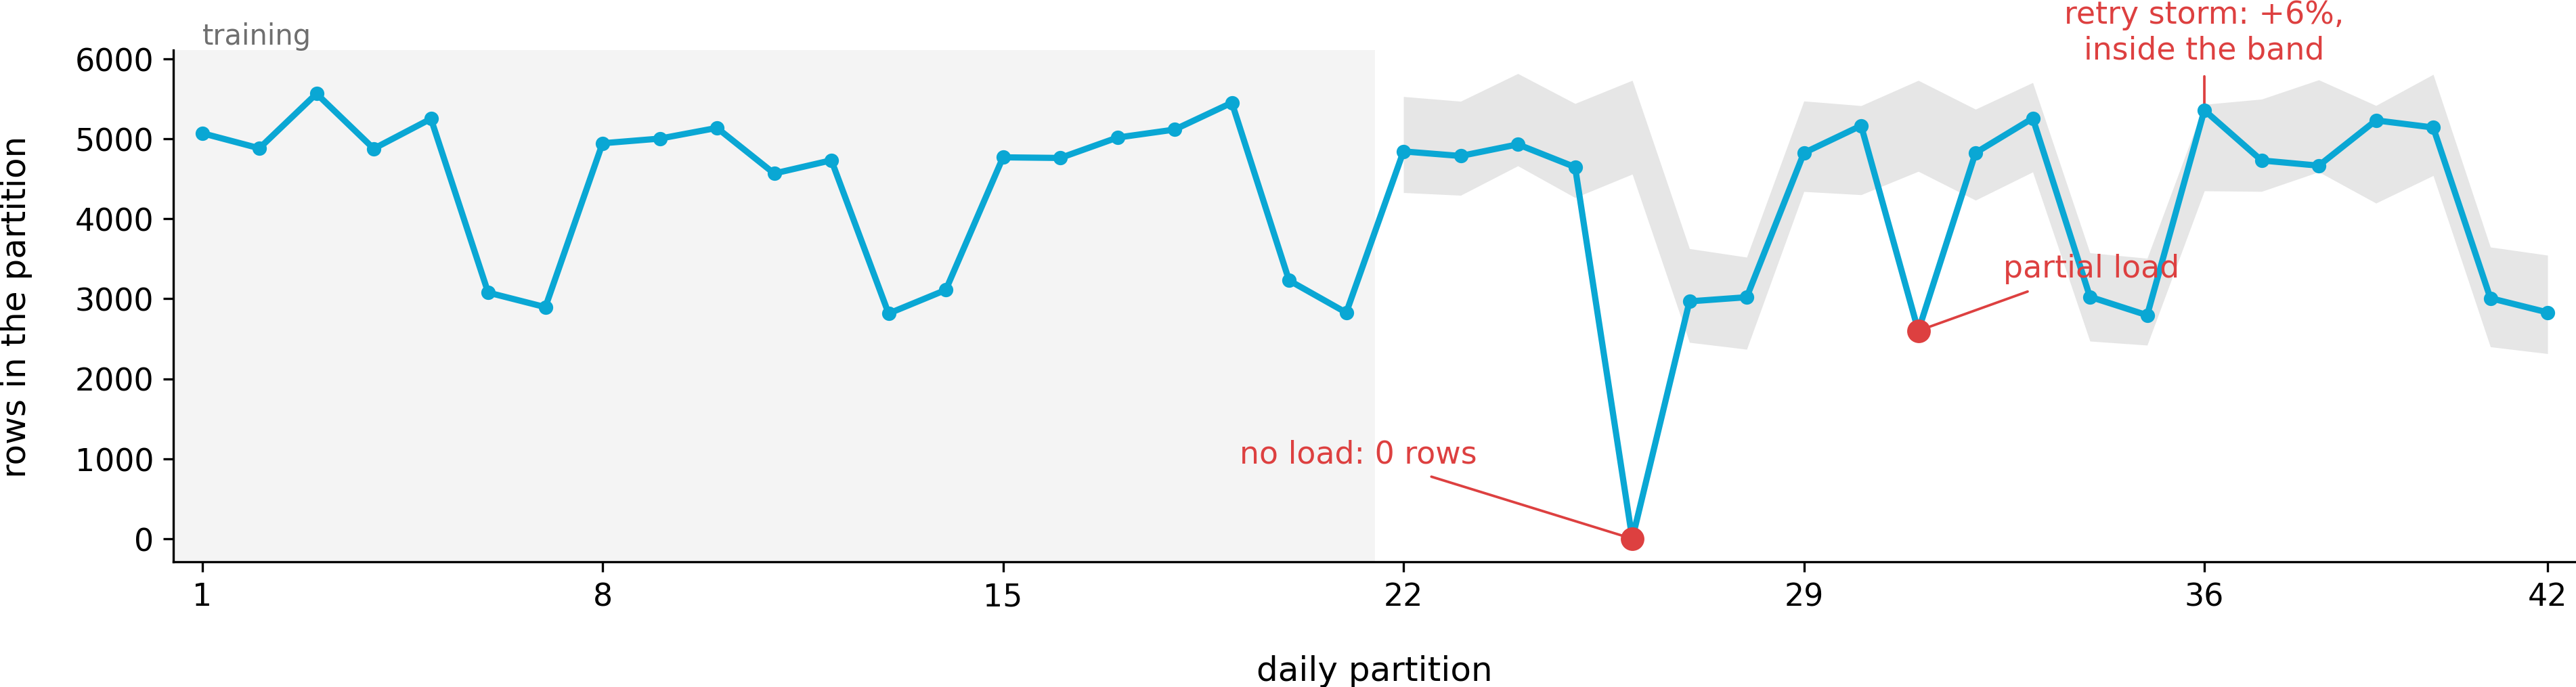
\includegraphics[width=\textwidth]{figures/Observability_row_count.png}
\end{center}

\textbf{Figure. Row Count.} Daily row counts for an orders table. Day $26$ has no rows and day $31$ has only $2{,}600$; both are below the expected range. On day $36$, some rows are loaded twice, bringing the count to $5{,}358$. That is still inside the range, so row count alone misses the repeated rows.

\textbf{When to use it?}

Use it to check whether a scheduled load delivered the expected amount of data. Compare equivalent periods and account for patterns such as quieter weekends. If rows can arrive late, recheck earlier days too. A normal count does not guarantee that the rows are correct or unique.

% ---------- Freshness ----------
\clearpage
\thispagestyle{observabilitystyle}
\section{Freshness}\label{sec:freshness}
\subsection{Most Recent Timestamp}

Freshness measures how much time has passed since the latest timestamp in a column. With an arrival timestamp, it tells you when data last reached the table. With an event timestamp, it tells you when the latest recorded event happened.

% equation
\begin{center}
    \tikz{
        \node[inner sep=2pt, font=\Large] (a) {
            {
                $\displaystyle
                \text{freshness}_t = {\color{nmlpurple}t_{\text{scan}}} - \max_{r \in T} {\color{nmlcyan}\text{ts}(r)}
                $
            }
        };
        \path[room for labels] ([yshift=0.57cm]a.north) ([yshift=-0.00cm]a.south);
        \draw[overlay,-latex,nmlpurple, semithick] ($(a.north)+(0.19,-0.09)$) to[bend right=15] node[pos=1, left] {time of the scan} +(-1.00,0.30);
        \draw[overlay,-latex,nmlcyan, semithick] ($(a.north)+(2.76,-0.03)$) to node[pos=1, above] {newest timestamp} +(0.00,0.30);
    }
\end{center}

The formula subtracts the newest timestamp from the scan time, ignoring nulls. If the latest arrival is at 01:30 and the scan is at 06:00, freshness is $4.5$ hours. Some databases also record when a table was last updated. That can be checked without reading its rows, but an update does not prove that newer data arrived.

\begin{center}
    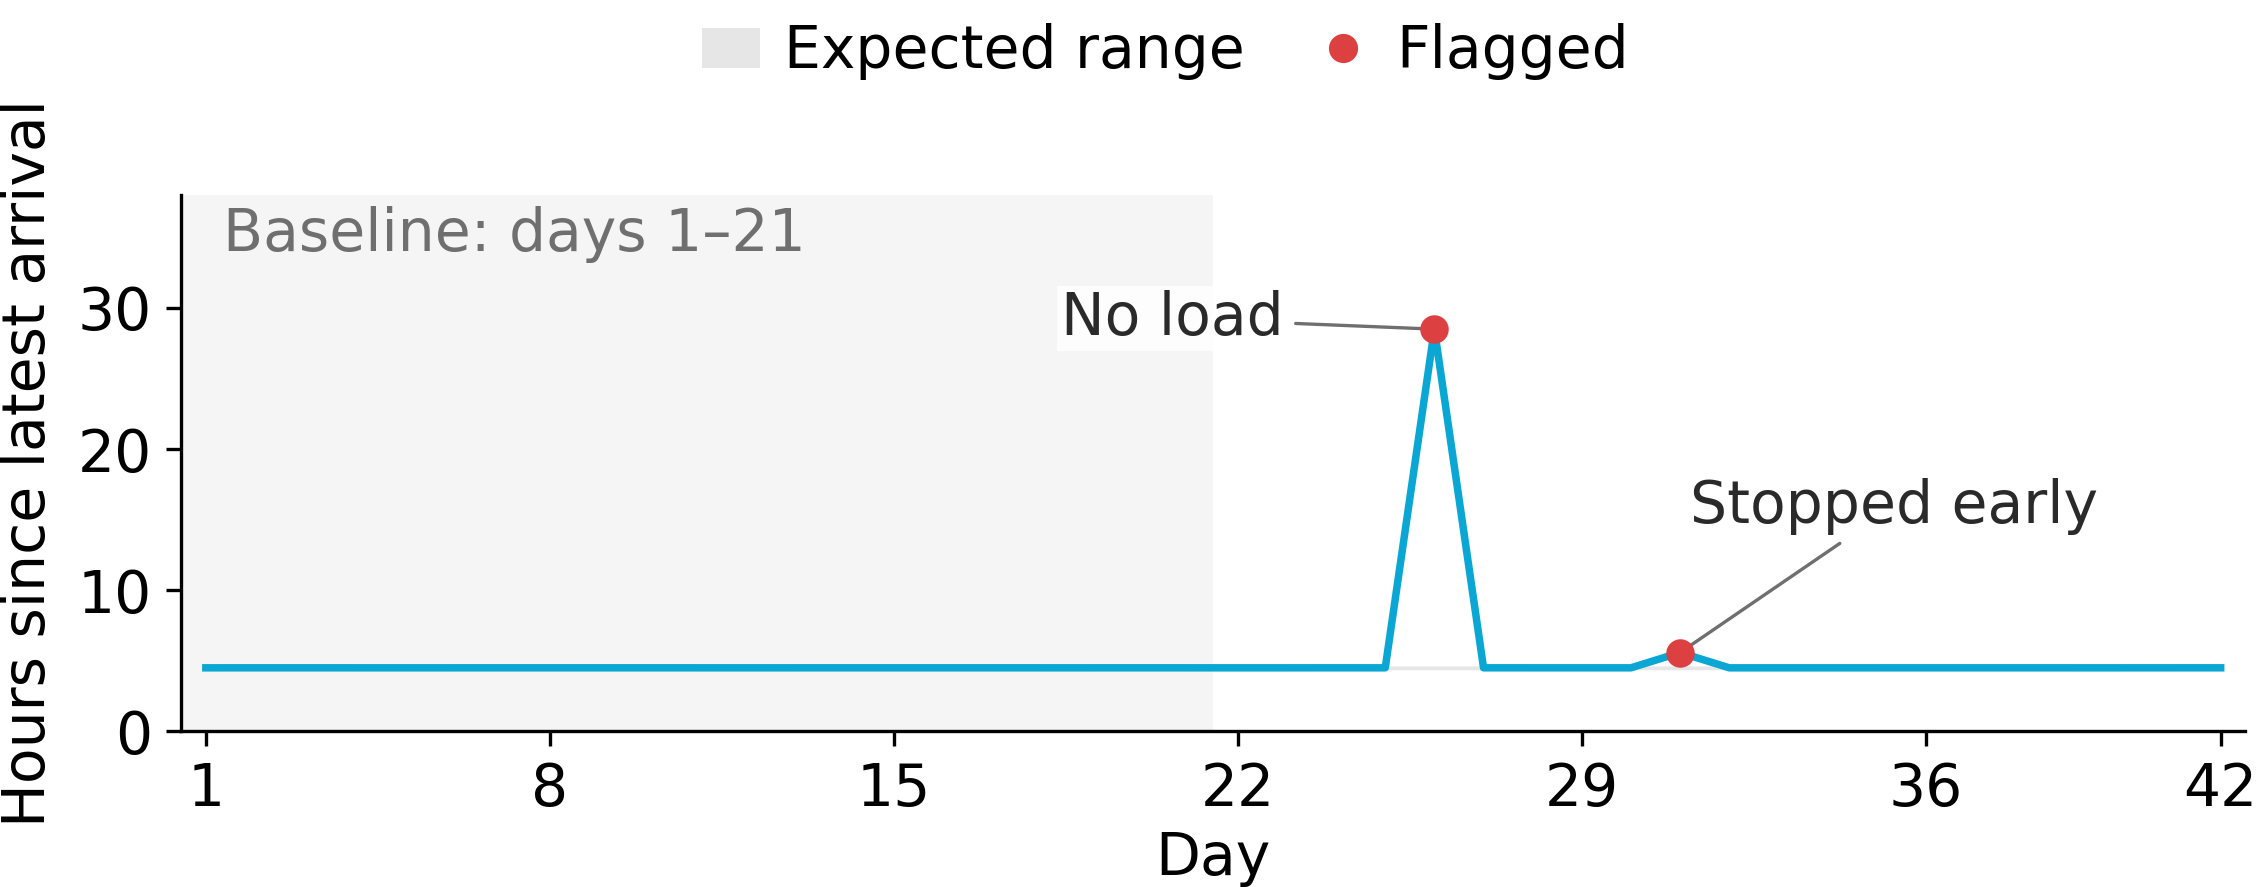
\includegraphics[width=\textwidth]{figures/Observability_freshness.png}
\end{center}

\textbf{Figure. Freshness.} The orders table is scanned at 06:00, usually $4.5$ hours after its latest arrival. Nothing arrives on day $26$, so freshness reaches $28.5$ hours. The load stops early on day $31$, leaving the newest row $5.6$ hours old. Both days are flagged.

\textbf{When to use it?}

Use it when data must arrive before a deadline. Choose the timestamp that matches what you need to check, and allow for the loading schedule and time zone. Check row count too: one recent row can make an incomplete load look fresh. Without a valid timestamp, freshness cannot be calculated.

% ---------- Schema Changes ----------
\clearpage
\thispagestyle{observabilitystyle}
\section{Schema Changes}\label{sec:schema-changes}
\subsection{Columns and Types}

Schema monitoring detects changes to column names and data types. It can tell you when a column is added, removed or given a different type. These changes may break queries or alter how values are stored, even when the data still loads successfully.

% equation
\begin{center}
    \tikz{
        \node[inner sep=2pt, font=\Large] (a) {
            {
                $\displaystyle
                \Delta_t = {\color{nmlcyan}S_t} \,\triangle\, {\color{nmlpurple}S_{t-1}}, \qquad \text{anomaly} \iff \Delta_t \neq \varnothing
                $
            }
        };
        \path[room for labels] ([yshift=0.50cm]a.north) ([yshift=-0.47cm]a.south);
        \draw[overlay,-latex,nmlcyan, semithick] ($(a.north)+(-3.34,-0.03)$) to node[pos=1, above] {columns and types now} +(0.00,0.22);
        \draw[overlay,-latex,nmlpurple, semithick] ($(a.south)+(-1.69,0.07)$) to node[pos=1, below] {at the previous scan} +(0.00,-0.22);
    }
\end{center}

Each $S$ lists the column names and types at one scan. The $\triangle$ compares two lists and keeps only the differences. A renamed column appears as one removal and one addition. The check flags changes for review; an intentional change is not necessarily a problem.

\begin{center}
    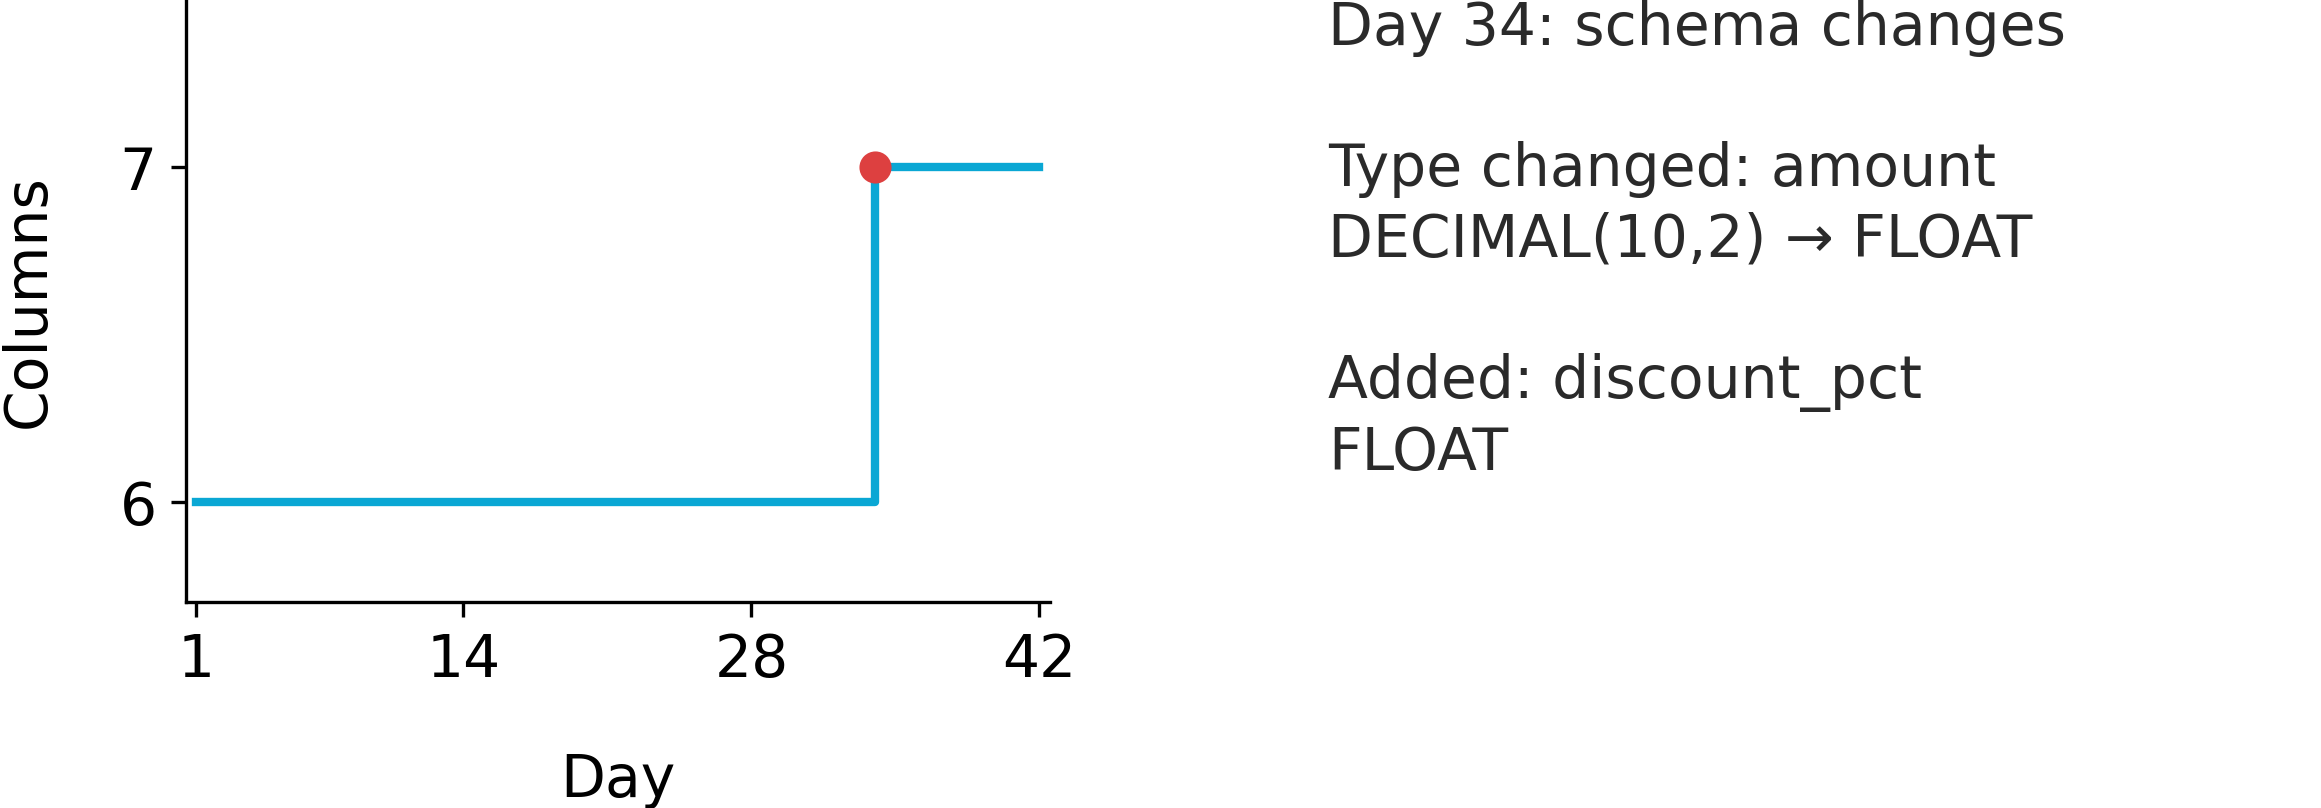
\includegraphics[width=\textwidth]{figures/Observability_schema.png}
\end{center}

\textbf{Figure. Schema Changes.} \underline{Left:} the table grows from six columns to seven on day $34$. \underline{Right:} \texttt{discount\_pct} is added and \texttt{amount} changes from \texttt{DECIMAL(10,2)} to \texttt{FLOAT}. The column count shows the addition, but only comparing the types reveals the second change.

\textbf{When to use it?}

Use it on tables that other queries, applications or models depend on. Check whether a change affects those uses before accepting it. Changes to the values themselves can go unnoticed: storing cents instead of dollars may leave the column name and type unchanged.

% ---------- Missing Values ----------
\clearpage
\thispagestyle{observabilitystyle}
\section{Missing Values}\label{sec:missing-values}
\subsection{Completeness}

Missing values percentage tells you what share of a column's values are null. It helps check whether needed information is present. For example, a rise in missing country codes may indicate that a source field is no longer being loaded correctly.

% equation
\begin{center}
    \tikz{
        \node[inner sep=2pt, font=\Large] (a) {
            {
                $\displaystyle
                \text{missing}\%_t = 100 \cdot \left( 1 - \frac{{\color{nmlcyan}\text{count}(c)}}{{\color{nmlred}\text{count}(*)}} \right)
                $
            }
        };
        \path[room for labels] ([yshift=0.24cm]a.north) ([yshift=-0.19cm]a.south);
        \draw[overlay,-latex,nmlcyan, semithick] ($(a.north)+(2.37,-0.04)$) to[bend right=15] node[pos=1, left] {non-null values in the column} +(-1.00,0.30);
        \draw[overlay,-latex,nmlred, semithick] ($(a.south)+(2.29,0.10)$) to[bend left=15] node[pos=1, left] {rows in the partition} +(-1.00,-0.30);
    }
\end{center}

The formula compares the number of filled rows, $\text{count}(c)$, with the total number of rows, $\text{count}(*)$. If $80$ of $100$ rows are filled, the missing percentage is $20\%$. This check counts nulls; blank text and placeholders such as \texttt{N/A} may need separate rules.

\begin{center}
    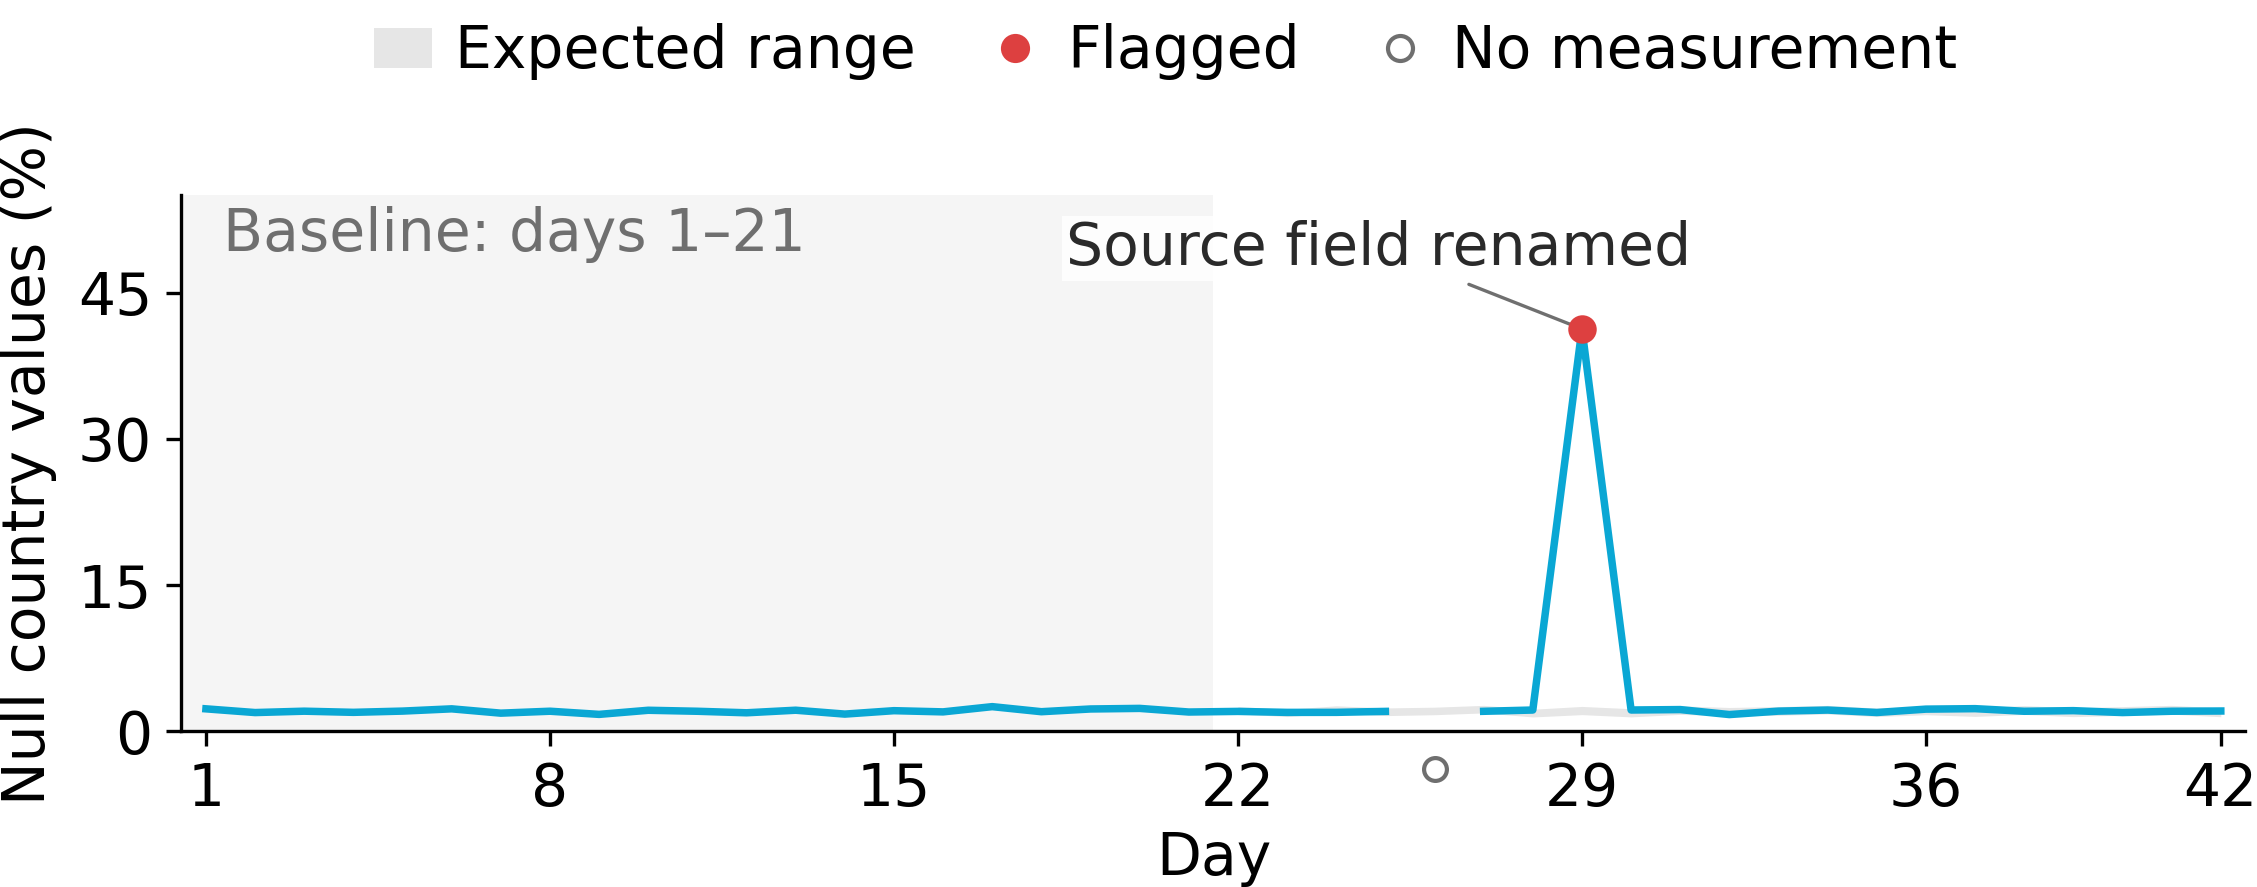
\includegraphics[width=\textwidth]{figures/Observability_missing.png}
\end{center}

\textbf{Figure. Missing Values.} About $2\%$ of country values are normally null. On day $29$, a source-field rename leaves $41\%$ missing, so the monitor flags the increase. The hollow point on day $26$ marks a day with no rows: there is no percentage to calculate.

\textbf{When to use it?}

Use it on fields needed for joins, reports or model inputs. Set the acceptable level according to the field: an optional field may legitimately contain nulls. Replacing missing values with a placeholder such as \texttt{unknown} can make the percentage fall without improving the data.

% ---------- Duplicates ----------
\clearpage
\thispagestyle{observabilitystyle}
\section{Duplicates}\label{sec:duplicates}
\subsection{Uniqueness}

Duplicate percentage shows what share of rows have a repeated key. A key is a value, such as an order ID, used to identify a record. Here, every copy counts as a duplicate, and rows with null keys are excluded.

% equation
\begin{center}
    \tikz{
        \node[inner sep=2pt, font=\Large] (a) {
            {
                $\displaystyle
                \text{dup}\%_t = 100 \cdot \frac{1}{{\color{nmlred}|R|}} \sum_{r \in R} \mathds{1}\big[\, {\color{nmlred}n(v_r)} > 1 \,\big]
                $
            }
        };
        \draw[overlay,-latex,nmlred, semithick] ($(a.south)+(-0.29,0.25)$) to node[pos=1, below] {records with a non-null value} +(0.00,-0.30);
        \draw[overlay,-latex,nmlred, semithick] ($(a.north)+(2.10,-0.33)$) to node[pos=1, above] {how often record $r$'s value occurs} +(0.00,0.33);
    }
\end{center}

The set $R$ contains rows with a key, and $n(v_r)$ counts how often each key appears. For keys $[101,101,205,\text{null},\text{null}]$, three rows have a key and two share $101$. The duplicate percentage is therefore $2/3 \approx 66.7\%$. Some tools count only the extra copies, so check their definition.

\begin{center}
    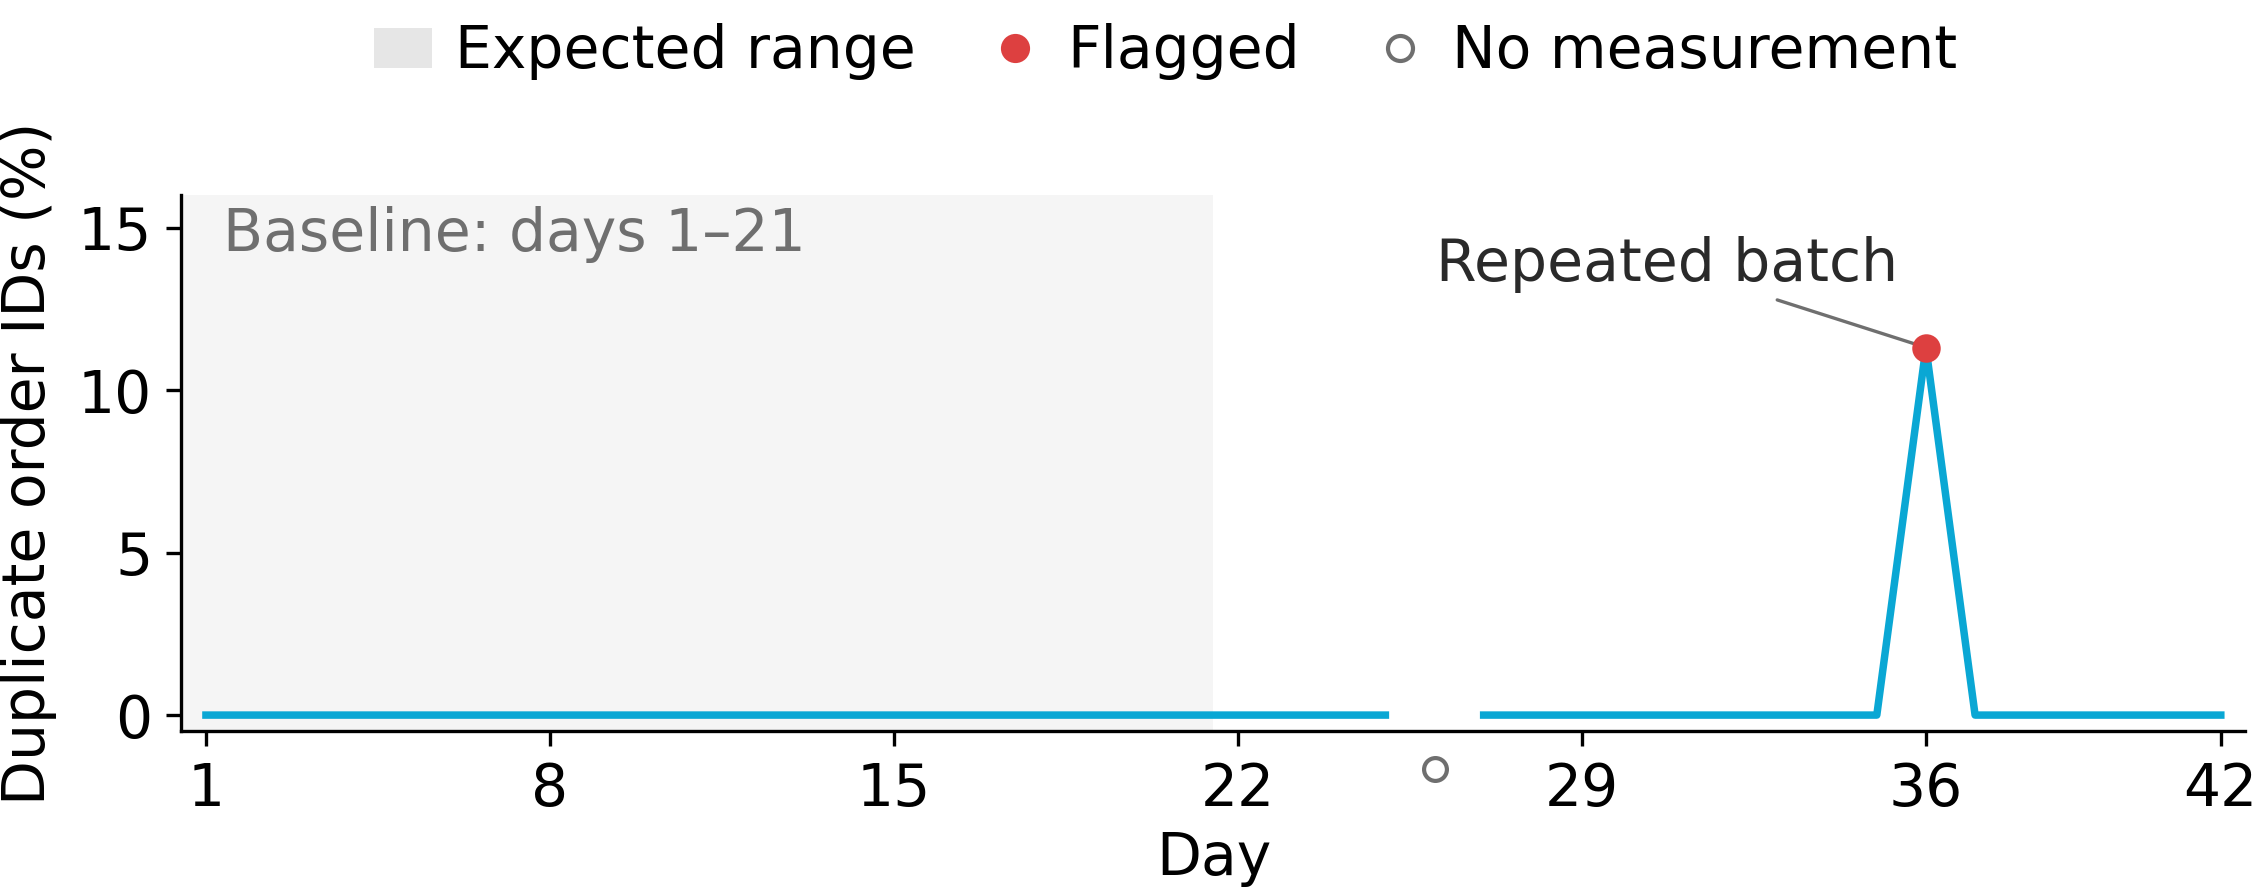
\includegraphics[width=\textwidth]{figures/Observability_duplicates.png}
\end{center}

\textbf{Figure. Duplicates.} Order IDs are unique except on day $36$, when $6\%$ of a load is inserted twice. For every $100$ original rows, six extra copies bring the total to $106$. The six originals and their copies make $12$ rows with repeated IDs: about $11.3\%$. The monitor flags this increase.

\textbf{When to use it?}

Use it on fields, or combinations of fields, that should identify rows uniquely. If any duplicate is an error, use a fixed limit of zero. Check missing keys separately. If keys must be unique across the whole table, checking only the latest day's rows is not enough.

% ---------- Unique Count ----------
\clearpage
\thispagestyle{observabilitystyle}
\section{Unique Count}\label{sec:unique-count}
\subsection{Cardinality}

Unique count tells you how many different values appear in a column. Each value counts once, even if it appears in many rows. Nulls are excluded. In an orders table, counting unique customer IDs tells you how many different customers placed an order.

% equation
\begin{center}
    \tikz{
        \node[inner sep=2pt, font=\Large] (a) {
            {
                $\displaystyle
                \text{unique}_t = \big|\, \{\, {\color{nmlcyan}c(r)} : r \in P_t,\; c(r) \neq \text{null} \,\} \,\big|
                $
            }
        };
        \path[room for labels] ([yshift=0.55cm]a.north) ([yshift=-0.00cm]a.south);
        \draw[overlay,-latex,nmlcyan, semithick] ($(a.north)+(-1.02,-0.09)$) to node[pos=1, above] {value of the column in row $r$} +(0.00,0.33);
    }
\end{center}

Here, $P_t$ is the group of rows being checked and $c(r)$ is the value in each row. For example, customer IDs $[101,101,205,\text{null}]$ give a unique count of $2$: only $101$ and $205$ are counted.

\begin{center}
    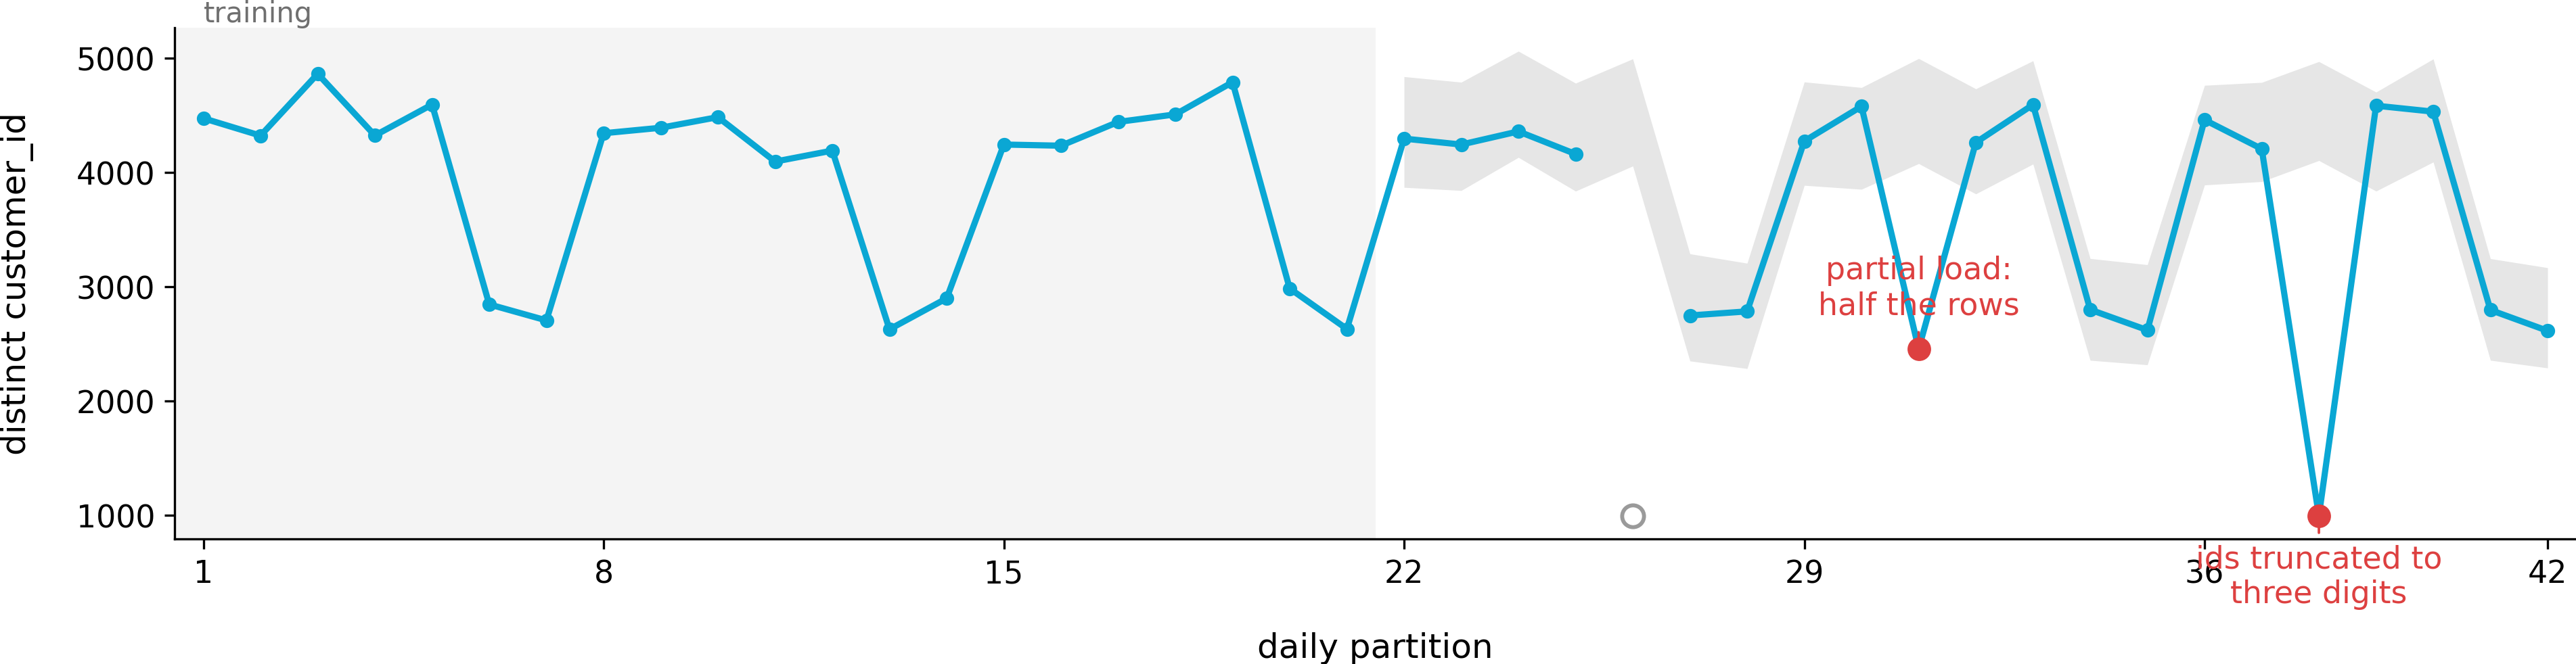
\includegraphics[width=\textwidth]{figures/Observability_unique_count.png}
\end{center}

\textbf{Figure. Unique Count.} Daily counts of different customer IDs. Weekends normally have fewer customers than weekdays. On day $31$, an incomplete load reduces the count. On day $38$, IDs are shortened to their last three digits, so different IDs become identical. Only $995$ unique values remain despite a normal load size. The hollow point marks day $26$, when no rows arrived and the check was skipped.

\textbf{When to use it?}

Use it to monitor customer IDs, product codes or categories such as countries. If unique count falls, check whether fewer rows arrived before investigating the values. It counts different values but does not tell you what they are: replacing one country code with another can leave the count unchanged.

% ---------- Average ----------
\clearpage
\thispagestyle{observabilitystyle}
\section{Average}\label{sec:average}
\subsection{Mean}

The average, or mean, is the sum of a column's values divided by how many values there are. Nulls are left out. Tracking the average can reveal a change in prices, quantities or other numeric data even when the row count stays the same.

% equation
\begin{center}
    \tikz{
        \node[inner sep=2pt, font=\Large] (a) {
            {
                $\displaystyle
                \bar{x}_t = \frac{1}{{\color{nmlred}n_t}} \sum_{r \in P_t} {\color{nmlcyan}x(r)}
                $
            }
        };
        \draw[overlay,-latex,nmlred, semithick] ($(a.south)+(-0.40,0.33)$) to node[pos=1, below] {non-null values in the partition} +(0.00,-0.30);
        \draw[overlay,-latex,nmlcyan, semithick] ($(a.north)+(1.30,-0.33)$) to[bend right=15] node[pos=1, left] {numeric value in row $r$} +(-1.00,0.61);
    }
\end{center}

Here, $n_t$ counts the values used in the calculation. For $[10,20,30]$, the average is $20$. A few very large values can raise it sharply. Increases and decreases can also cancel out, so the same average can describe very different data.

\begin{center}
    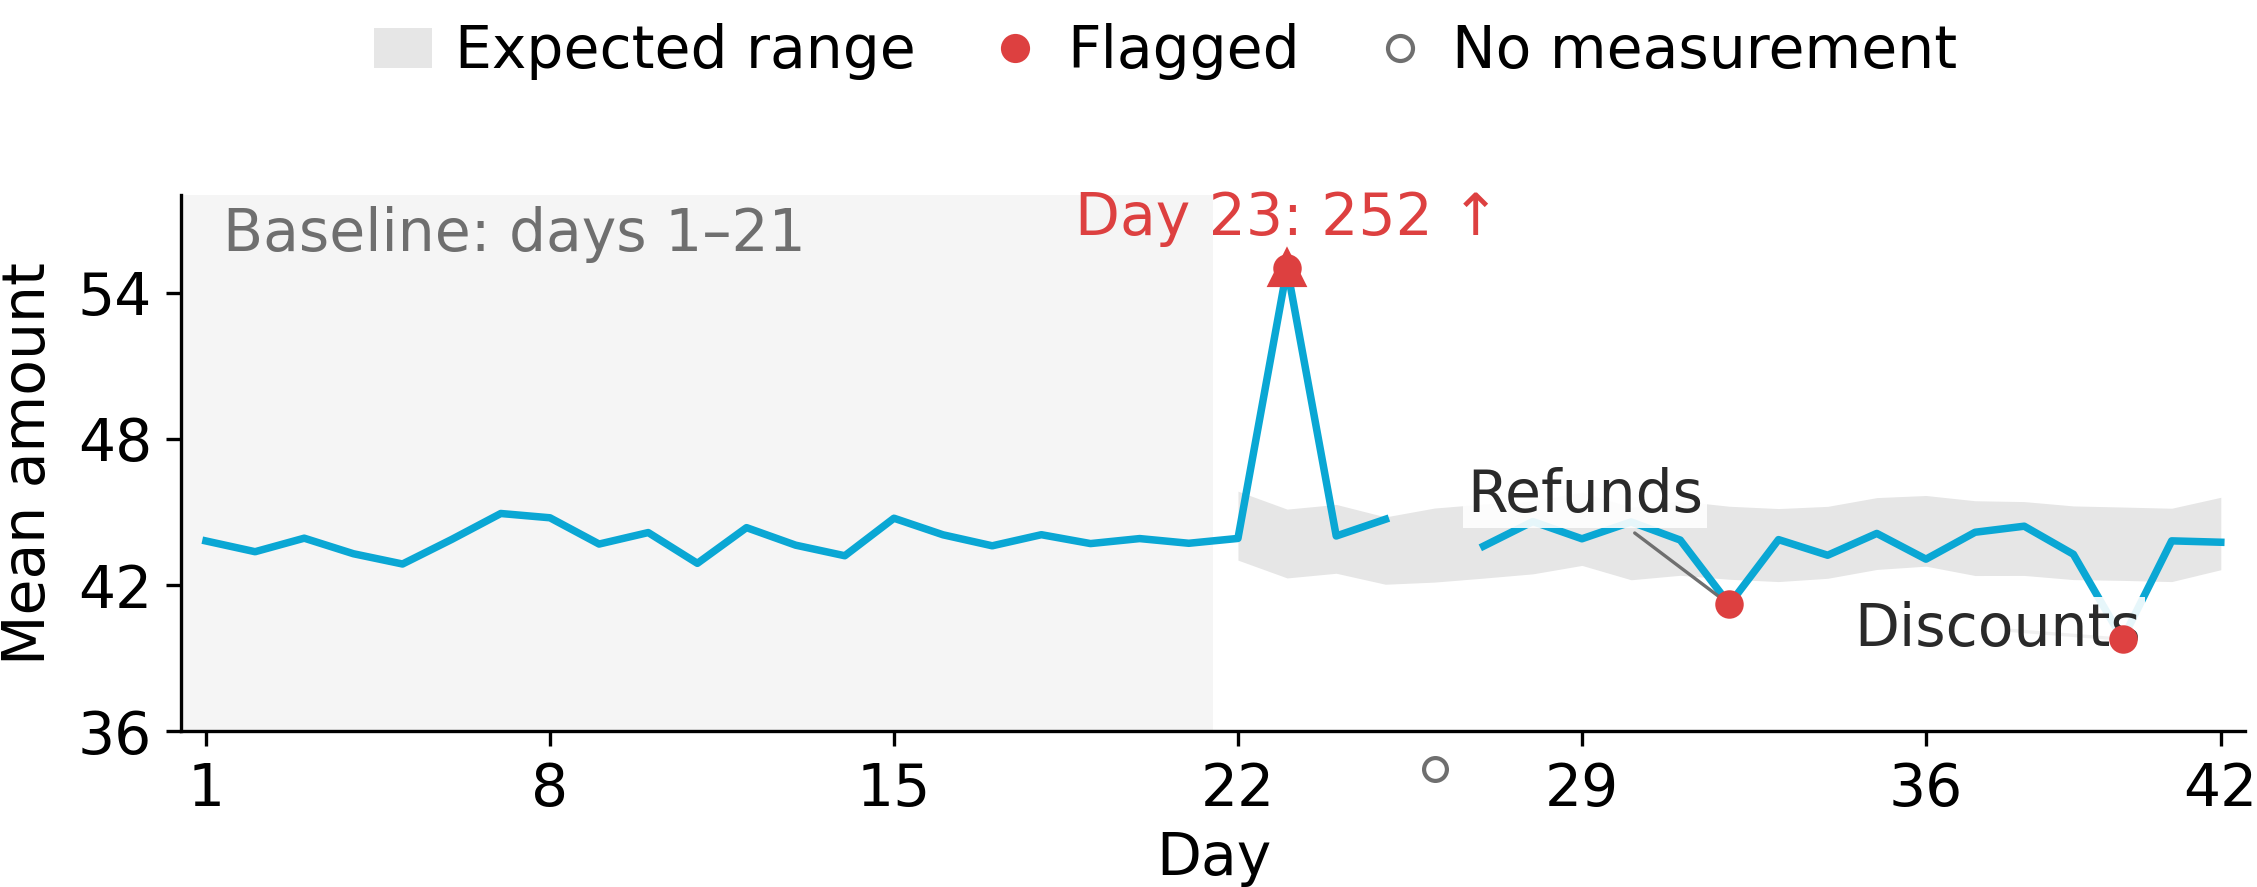
\includegraphics[width=\textwidth]{figures/Observability_average.png}
\end{center}

\textbf{Figure. Average.} Daily mean order amount. On day $23$, about $5\%$ of amounts arrive in cents instead of currency units. The mean rises from about $44$ to $252$, above the plotted scale. Negative refunds on day $32$ and discounts on amounts below $30$ on day $40$ lower the mean. All three changes are flagged.

\textbf{When to use it?}

Use it to track the overall level of a numeric column. Check quartiles and spread to understand what changed. The median is less affected by a few extreme values. A change in the average can also be legitimate, for example during a promotion.

% ---------- Sum ----------
\clearpage
\thispagestyle{observabilitystyle}
\section{Sum}\label{sec:sum}
\subsection{Total}

The sum adds up the values in a numeric column, ignoring nulls. It can track daily revenue or total units sold. A total can change because more rows arrived, because the values changed, or both.

% equation
\begin{center}
    \tikz{
        \node[inner sep=2pt, font=\Large] (a) {
            {
                $\displaystyle
                \Sigma_t = \sum_{r \in P_t} {\color{nmlcyan}x(r)} = {\color{nmlred}n_t} \cdot {\color{nmlpurple}\bar{x}_t}
                $
            }
        };
        \draw[overlay,-latex,nmlcyan, semithick] ($(a.north)+(-0.2,-0.2)$) to[bend right=15] node[pos=1, left] {numeric value in row $r$} +(-0.8,.5);
        \draw[overlay,-latex,nmlred, semithick] ($(a.south)+(1.4,0.3)$) to[bend left=15] node[pos=1, left] {rows} +(-0.4,-.5);
        \draw[overlay,-latex,nmlpurple, semithick] ($(a.north)+(2.2,-0.2)$) to[bend left=15] node[pos=1, right] {mean} +(0.6,.5);
    }
\end{center}

The sum also equals the number of non-null values $n_t$ times their average $\bar{x}_t$. For $[10,20,30]$, the total is $60$: three values with an average of $20$. SQL \texttt{SUM} returns null when there are no values to add.

\begin{center}
    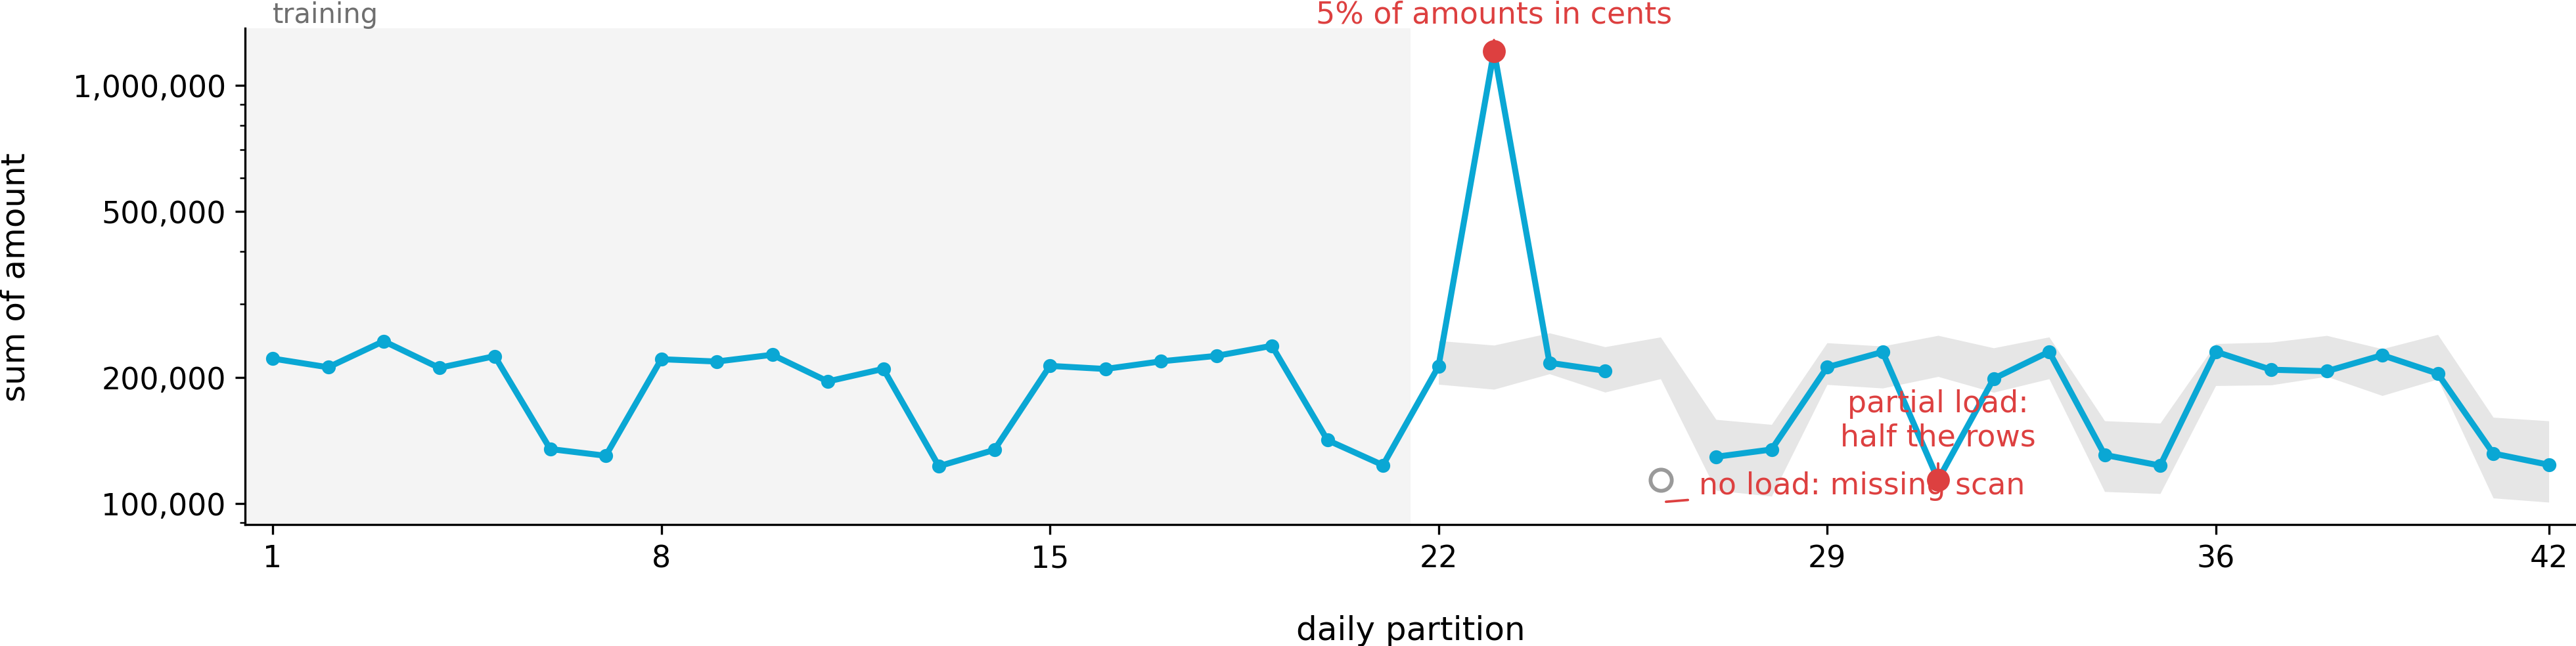
\includegraphics[width=\textwidth]{figures/Observability_sum.png}
\end{center}

\textbf{Figure. Sum.} Daily total order amount. On day $23$, about $5\%$ of amounts are stored in cents, making the total roughly six times larger. The incomplete load on day $31$ roughly halves it. Discounts on day $40$ do not push the total outside its expected range: daily changes in volume make this smaller change harder to detect.

\textbf{When to use it?}

Use it when a report depends on a total. To investigate an alert, check the number of filled rows and their average. A normal total can hide a problem if fewer rows contain larger values, or more rows contain smaller ones.

% ---------- Standard Deviation ----------
\clearpage
\thispagestyle{observabilitystyle}
\section{Standard Deviation}\label{sec:standard-deviation}
\subsection{Spread}

Standard deviation measures how much numeric values vary around their average. A larger value means they are more spread out; zero means they are all the same. It is expressed in the same units as the original values.

% equation
\begin{center}
    \tikz{
        \node[inner sep=2pt, font=\Large] (a) {
            {
                $\displaystyle
                s_t = \sqrt{ \frac{1}{{\color{nmlred}n_t} - 1} \sum_{r \in P_t} \big( {\color{nmlcyan}x(r)} - {\color{nmlpurple}\bar{x}_t} \big)^2 }
                $
            }
        };
        \draw[overlay,-latex,nmlred, semithick] ($(a.south)+(-0.9,0.3)$) to[bend left=15] node[pos=1, left] {non-null values} +(-0.6,-.5);
        \draw[overlay,-latex,nmlcyan, semithick] ($(a.north)+(1.0,-0.2)$) to[bend right=15] node[pos=1, left] {value in row $r$} +(-0.8,.5);
        \draw[overlay,-latex,nmlpurple, semithick] ($(a.north)+(2.3,-0.2)$) to[bend left=15] node[pos=1, right] {partition mean} +(0.6,.5);
    }
\end{center}

For example, $[20,20,20]$ and $[10,20,30]$ both average $20$, but only the second set has any spread. The formula gives the sample standard deviation and needs at least two non-null values. Some tools use the population version, which divides by $n_t$ rather than $n_t-1$.

\begin{center}
    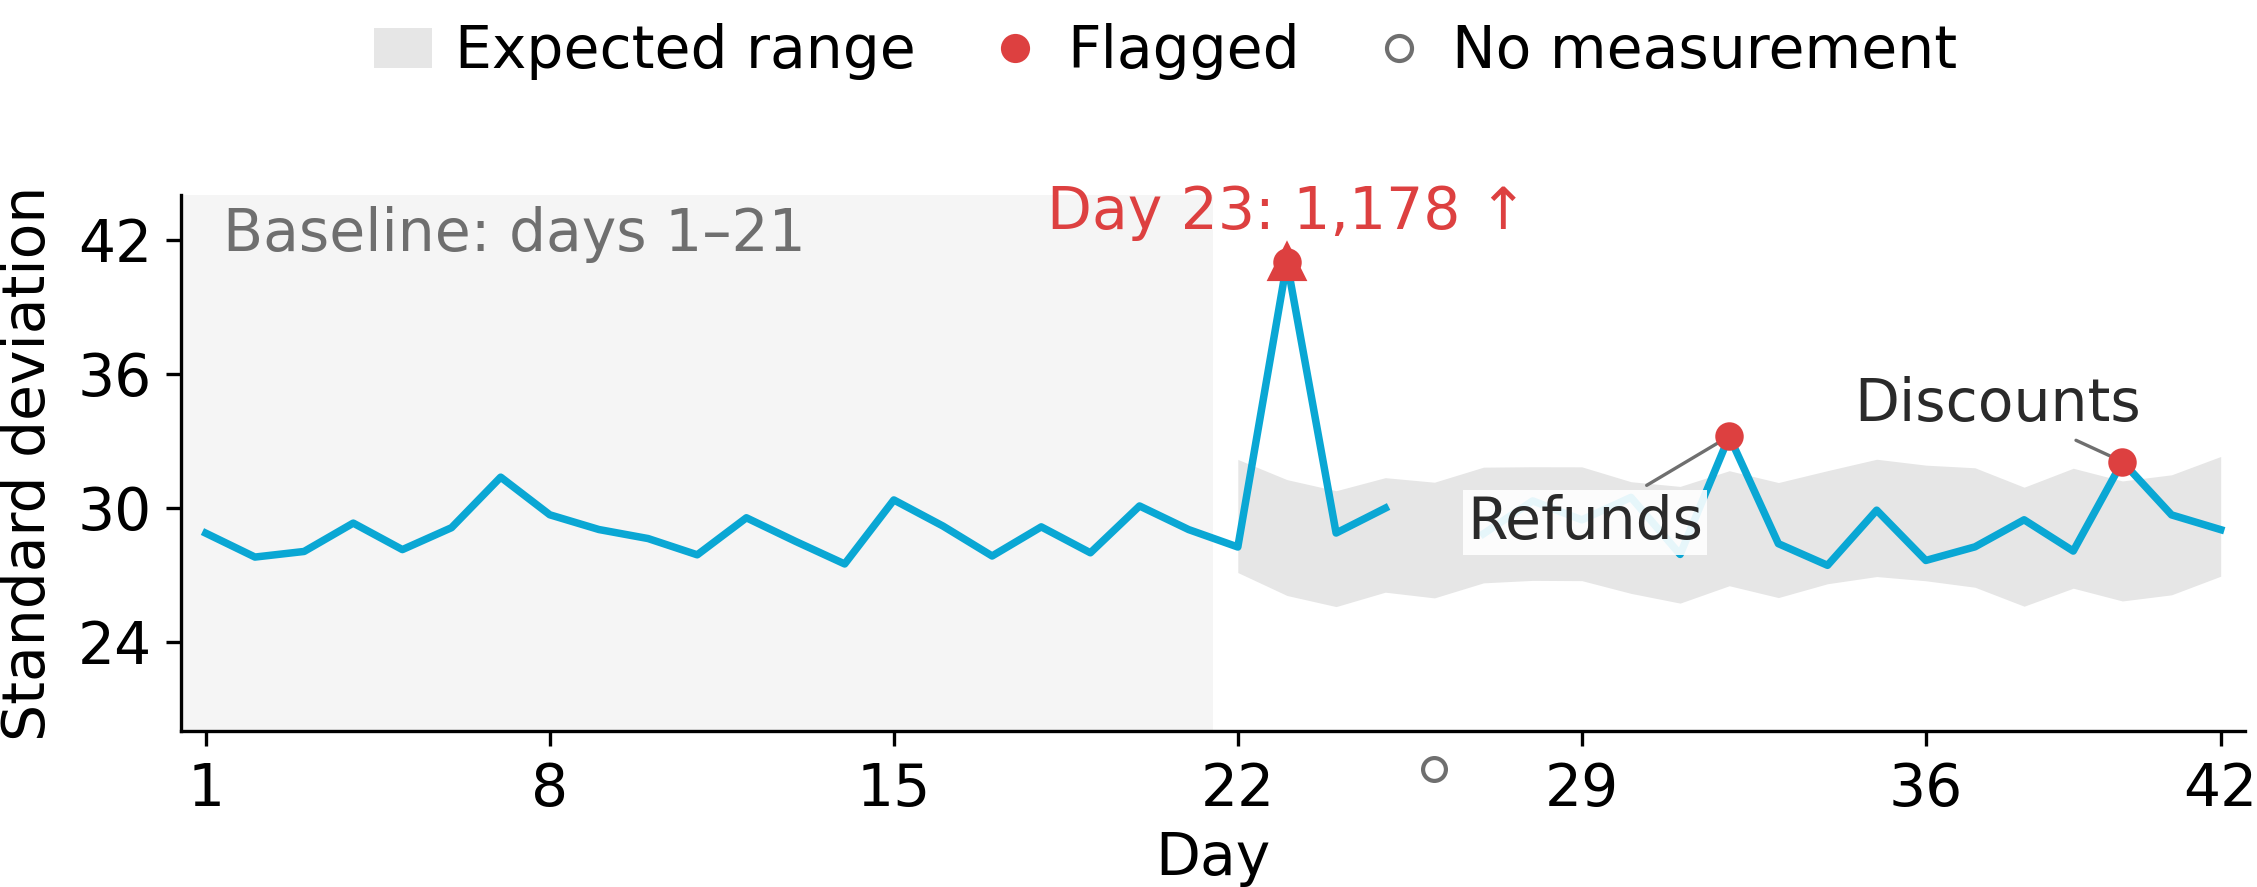
\includegraphics[width=\textwidth]{figures/Observability_stddev.png}
\end{center}

\textbf{Figure. Standard Deviation.} Daily spread of order amounts. On day $23$, about $5\%$ of amounts arrive in cents, increasing the spread about fortyfold, above the plotted scale. Negative refunds on day $32$ and discounts on amounts below $30$ on day $40$ also increase the spread. All three days are flagged.

\textbf{When to use it?}

Use it alongside the average to check how widely values vary. A few extreme values can strongly affect it, so inspect them before treating an alert as an error. Quartiles are less affected by those extremes and help show whether most values have changed.

% ---------- Min / Max ----------
\clearpage
\thispagestyle{observabilitystyle}
\section{Min and Max}\label{sec:min-and-max}
\subsection{Range}

Minimum and maximum are the smallest and largest values in a column, ignoring nulls. They help detect extreme values that an average can hide. For example, a single negative quantity changes the minimum even if thousands of other quantities are valid.

% equation
\begin{center}
    \tikz{
        \node[inner sep=2pt, font=\Large] (a) {
            {
                $\displaystyle
                \min_t = \min_{r \in P_t} {\color{nmlcyan}x(r)}, \qquad \max_t = \max_{r \in P_t} {\color{nmlpurple}x(r)}
                $
            }
        };
        \draw[overlay,-latex,nmlcyan, semithick] ($(a.north)+(-1.17,-0.04)$) to node[pos=1, above] {smallest non-null value} +(0.00,0.30);
        \draw[overlay,-latex,nmlpurple, semithick] ($(a.north)+(3.74,-0.04)$) to node[pos=1, above] {largest non-null value} +(0.00,0.30);
    }
\end{center}

The formula takes both values from the rows in $P_t$, the partition being checked. Only one row determines each result. That makes these checks sensitive to individual errors, but also to legitimate extremes, such as an unusually large order.

\begin{center}
    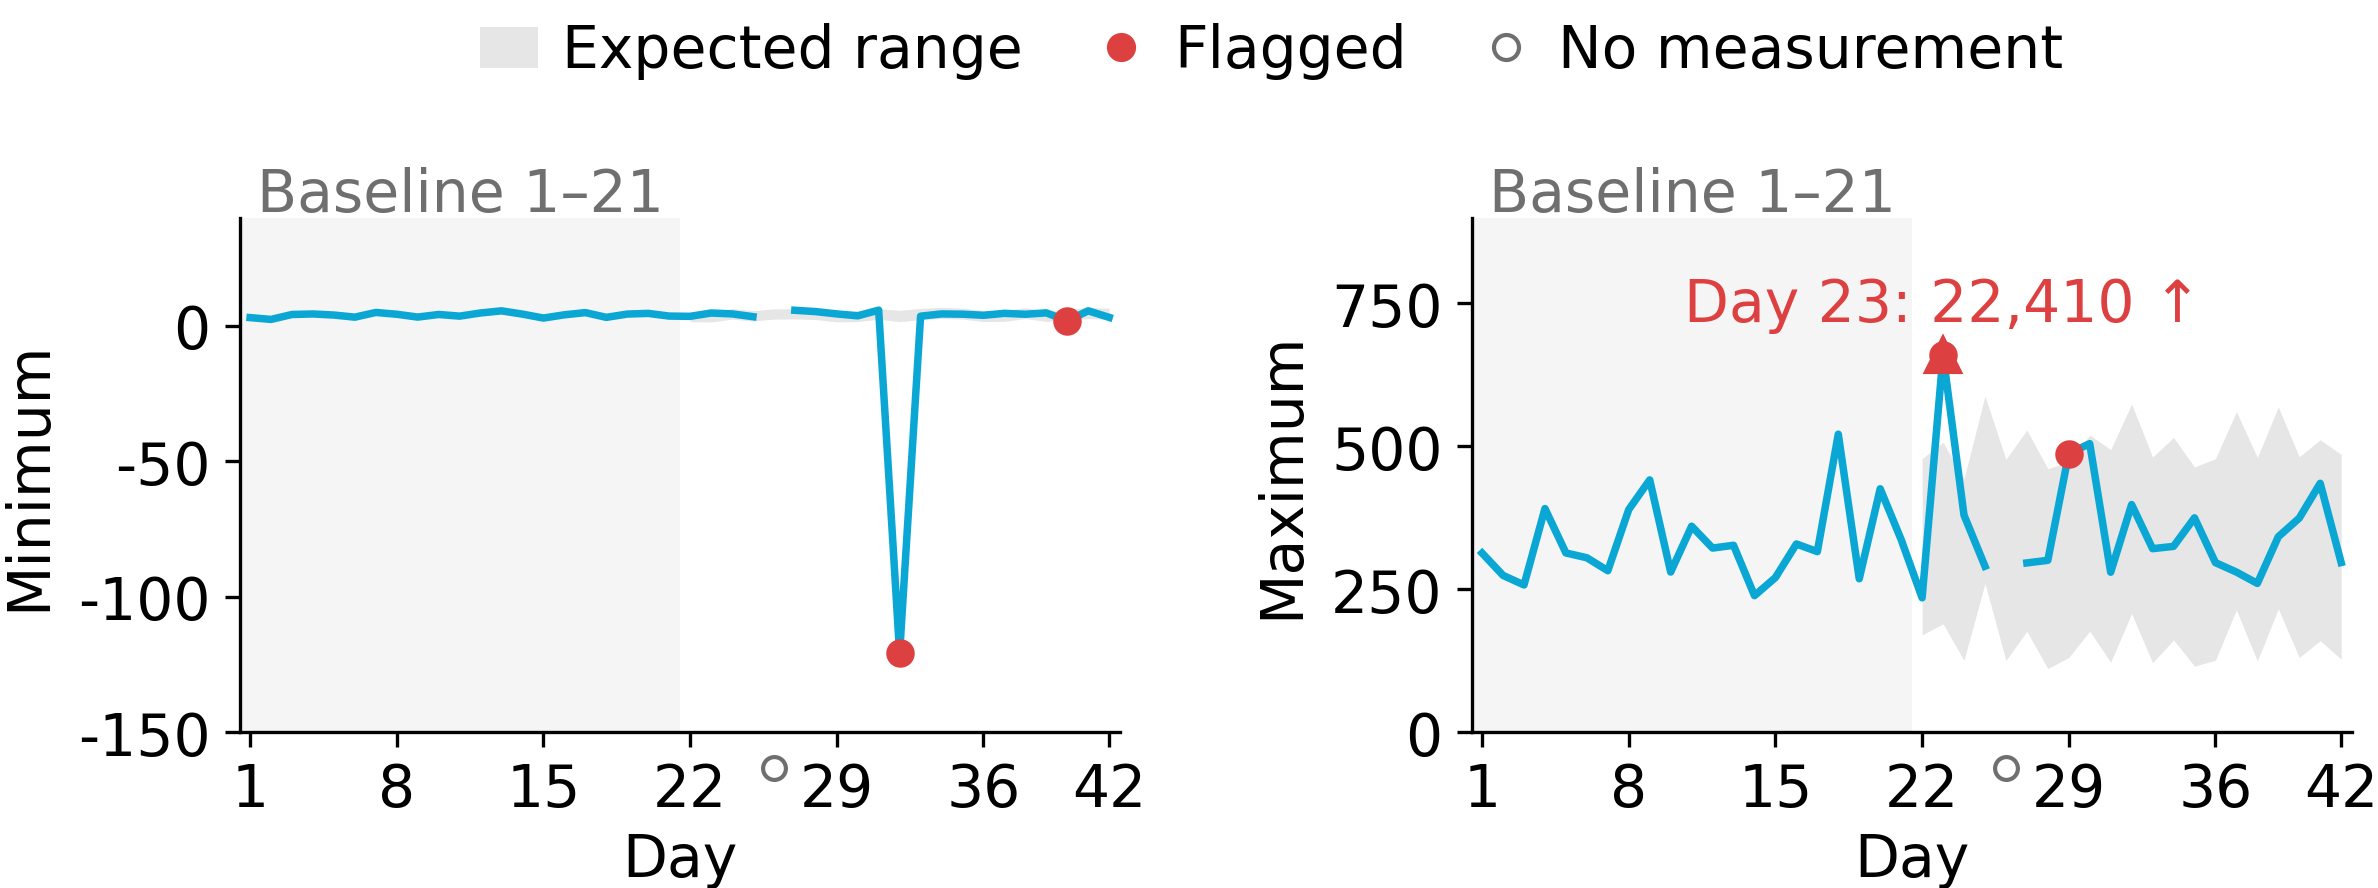
\includegraphics[width=\textwidth]{figures/Observability_min_max.png}
\end{center}

\textbf{Figure. Min and Max.} Daily order amounts. \underline{Left:} refunds on day $32$ produce a minimum of $-121$; discounts on day $40$ lower the minimum to $1.86$. \underline{Right:} amounts stored in cents on day $23$ raise the maximum to $22{,}410$, above the scale. Day $29$ also triggers an alert, but its $487$ order is valid.

\textbf{When to use it?}

Use fixed limits for known requirements, such as non-negative quantities. Use historical ranges when you want to spot unusual extremes, allowing for legitimate large or small values. Min and Max show the extremes, not how many rows are affected; count invalid rows separately if that matters.

% ---------- Quartiles ----------
\clearpage
\thispagestyle{observabilitystyle}
\section{Quartiles}\label{sec:quartiles}
\subsection{Q1, Median, Q3}

Quartiles mark three positions in a column's sorted values: one-quarter of the way through, halfway through, and three-quarters of the way through. These are Q1, the median and Q3. They help show where most values lie without being dominated by a few extremes.

% equation
\begin{center}
    \tikz{
        \node[inner sep=2pt, font=\Large] (a) {
            {
                $\displaystyle
                Q_{{\color{nmlyellow}p}}(t) = \inf \big\{\, x : {\color{nmlcyan}F_t}(x) \geq {\color{nmlyellow}p} \,\big\}, \qquad p \in \{0.25, 0.5, 0.75\}
                $
            }
        };
        \draw[overlay,-latex,nmlcyan, semithick] ($(a.south)+(-1.76,0.15)$) to node[pos=1, below] {share of values at or below $x$} +(0.00,-0.30);
        \draw[overlay,-latex,nmlyellow, semithick] ($(a.south)+(-0.21,0.13)$) to[bend right=15] node[pos=1, right] {the quantile level} +(1.00,-0.33);
    }
\end{center}

The function $F_t(x)$ gives the share of values at or below $x$, ignoring nulls. For Q1, the formula finds where that share first reaches $25\%$; the median and Q3 use $50\%$ and $75\%$. Software may estimate positions between observed values; these figures use linear interpolation.

\begin{center}
    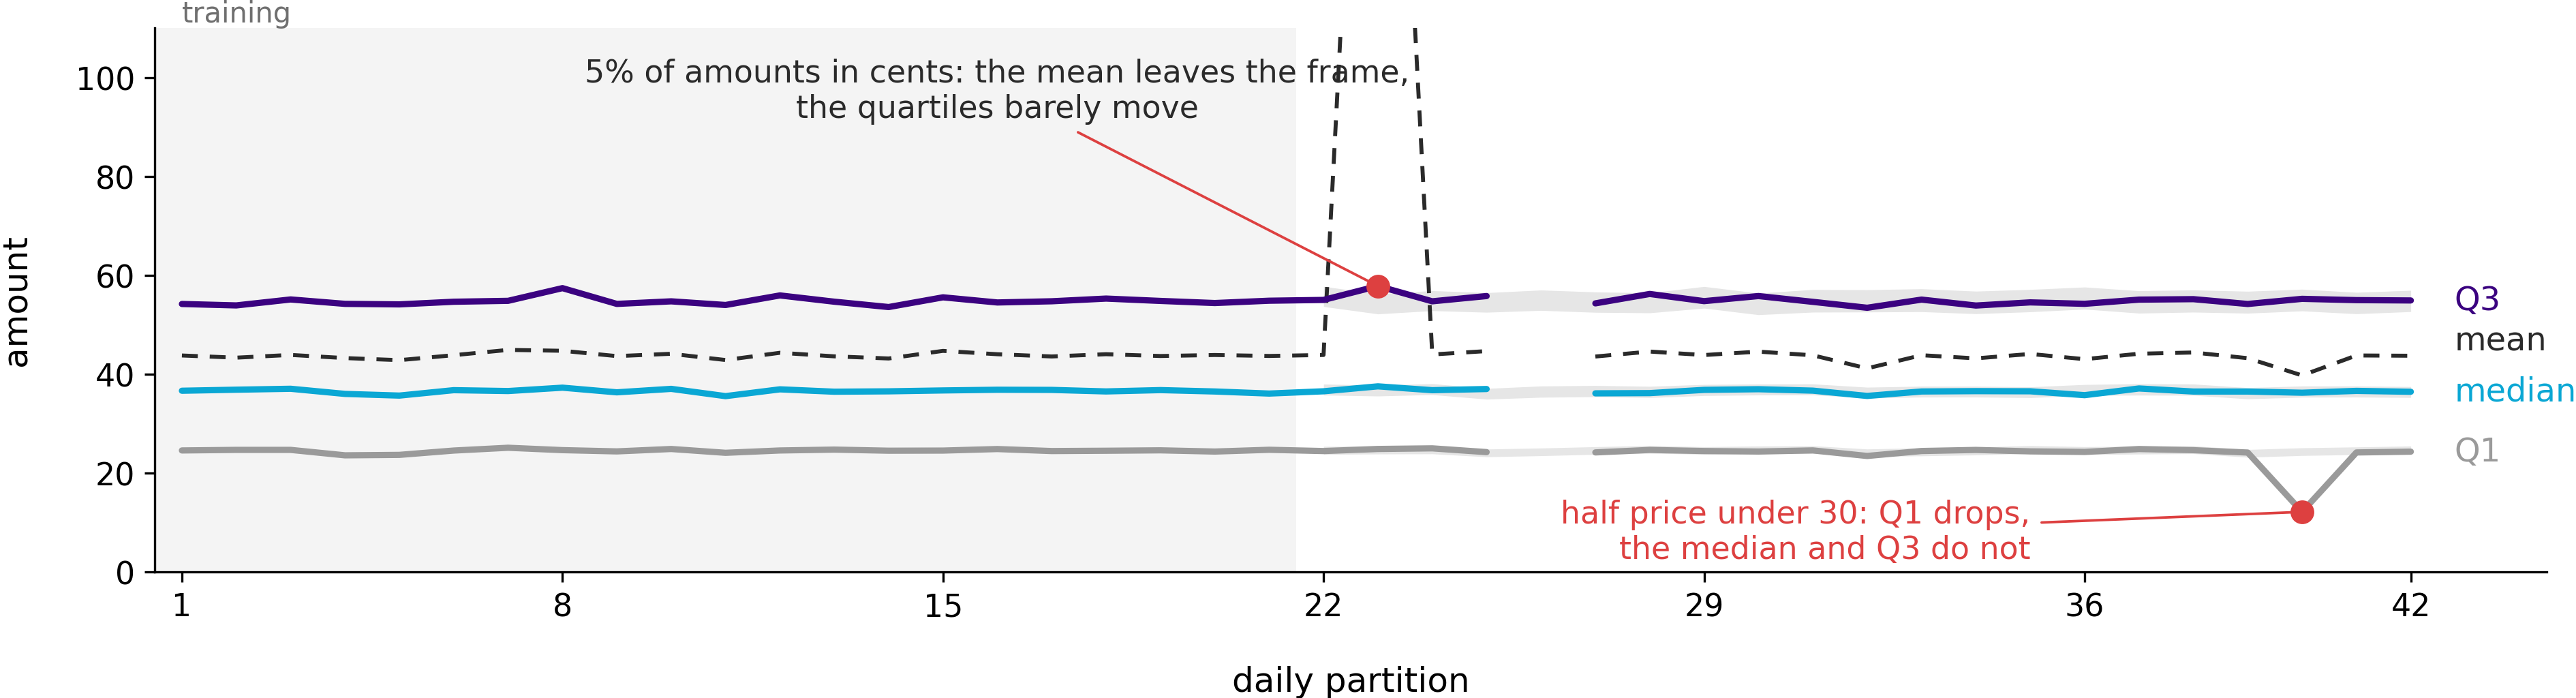
\includegraphics[width=\textwidth]{figures/Observability_quartiles.png}
\end{center}

\textbf{Figure. Quartiles.} Daily order-amount quartiles, with the mean dashed. On day $23$, about $5\%$ of amounts arrive in cents. The mean rises above the scale; Q3 rises much less but is still flagged. On day $40$, prices below $30$ are halved. Q1 drops from about $25$ to $12$; that day's median and Q3 are unaffected.

\textbf{When to use it?}

Use quartiles to track typical values and spread when a few large or small values make the mean hard to interpret. The gap between Q1 and Q3 shows the spread of the middle half of the data. Check Min and Max too if extreme values matter.

% ---------- Text Length ----------
\clearpage
\thispagestyle{observabilitystyle}
\section{Text Length}\label{sec:text-length}
\subsection{Format}

Text length counts the characters in a value. Tracking the average, shortest and longest lengths can reveal cut-off text, missing prefixes or changes in code format. Nulls are excluded, but an empty string has length zero.

% equation
\begin{center}
    \tikz{
        \node[inner sep=2pt, font=\Large] (a) {
            {
                $\displaystyle
                \overline{\ell}_t = \frac{1}{{\color{nmlred}n_t}} \sum_{r \in P_t} {\color{nmlcyan}\text{len}}\big(s(r)\big)
                $
            }
        };
        \path[room for labels] ([yshift=0.30cm]a.north) ([yshift=-0.00cm]a.south);
        \draw[overlay,-latex,nmlred, semithick] ($(a.south)+(-0.99,0.33)$) to[bend left=15] node[pos=1, left] {non-null strings} +(-1.00,-0.30);
        \draw[overlay,-latex,nmlcyan, semithick] ($(a.north)+(0.56,-0.34)$) to[bend right=15] node[pos=1, left] {characters in the string} +(-1.00,0.62);
    }
\end{center}

The formula adds the lengths of the non-null strings and divides by their count $n_t$. For lengths $[4,4,7]$, the average is $5$. Count characters rather than bytes: some characters occupy more than one byte.

\begin{center}
    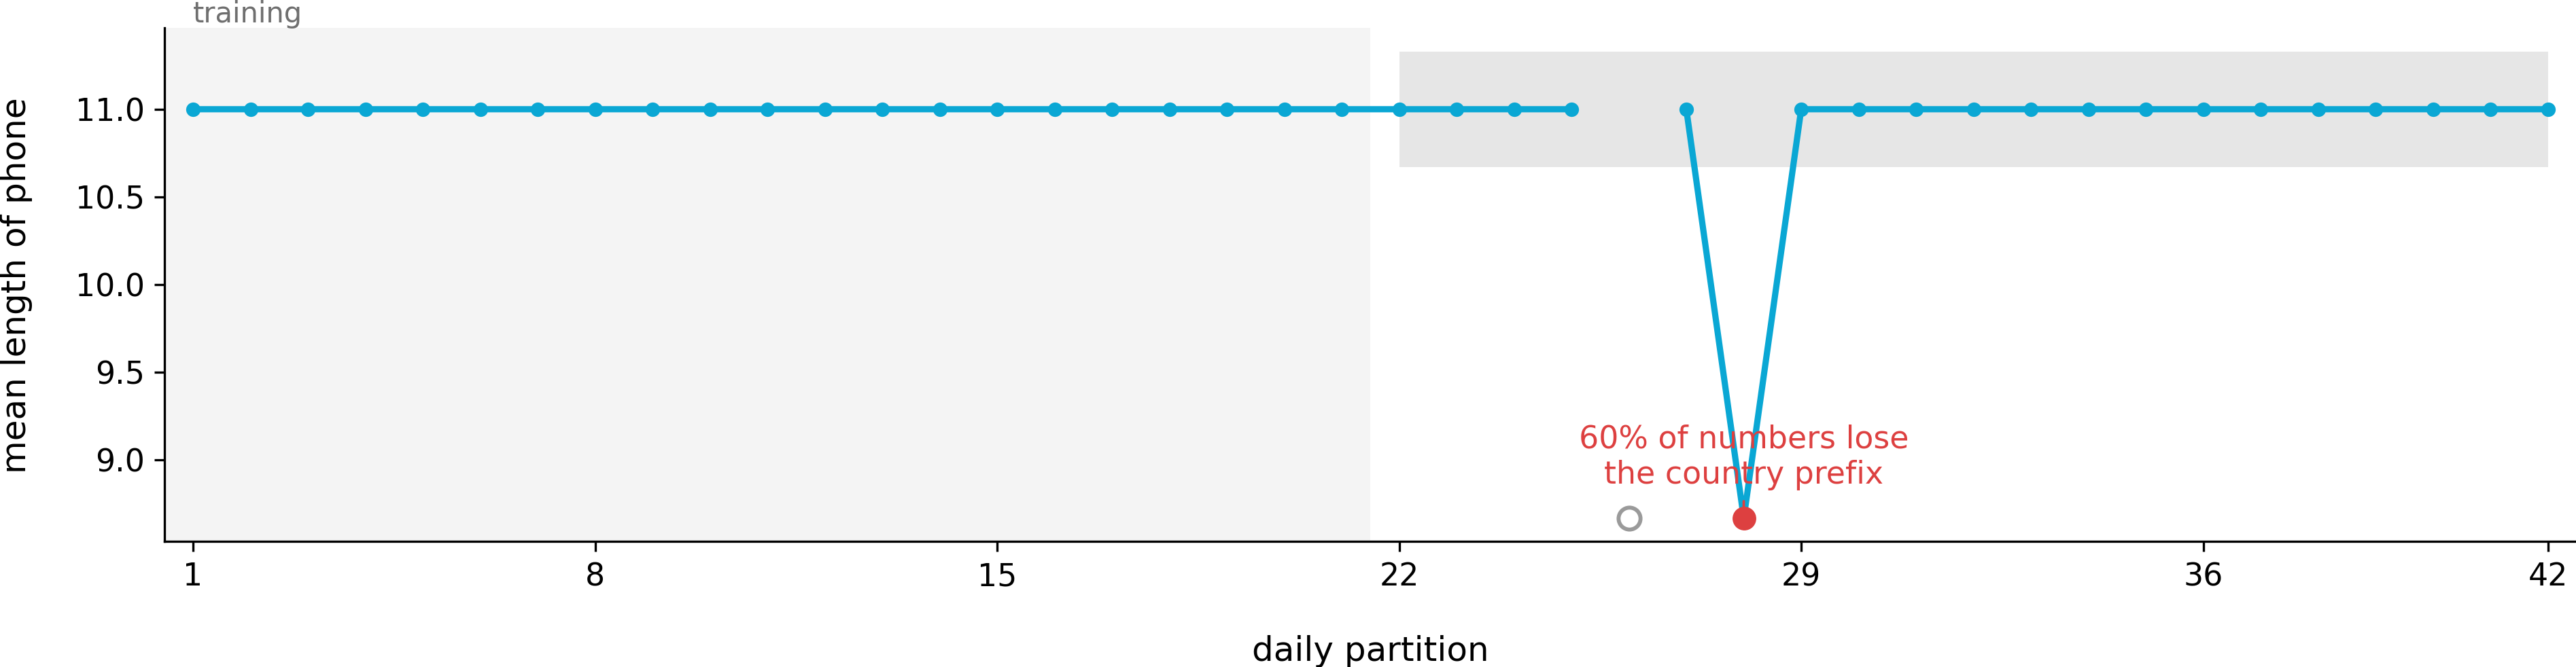
\includegraphics[width=\textwidth]{figures/Observability_text_length.png}
\end{center}

\textbf{Figure. Text Length.} Daily average length of phone values. They normally contain eleven characters, including punctuation. On day $28$, about $60\%$ arrive as seven-character values, reducing the average to $8.7$. The values are still text and none is null, so type and missing-value checks would not catch the change.

\textbf{When to use it?}

Use it on fields with a predictable format, such as product codes and phone numbers. Length alone cannot tell you whether the content is correct: two different values can have the same length. For free text, allow for normal variation before interpreting a change as an error.

\clearpage
\refstepcounter{chapter}
\addcontentsline{toc}{chapter}{\texorpdfstring{\protect\tocmark{cyanaccent}}{}Bibliography}
\renewcommand{\chaptertitle}{Bibliography}
\renewcommand{\sectiontitle}{}
\pagestyle{plain}
\noindent{\Huge\bfseries Bibliography\par}
\vspace{0.5em}

\begingroup
\small
\raggedright
\interlinepenalty=10000 % Keep each reference together across page breaks.
\setlength{\parskip}{5pt}
\newcommand{\srchead}[1]{\par\addvspace{10pt}\noindent{\normalsize\bfseries #1}\par\nobreak\vspace{2pt}\nobreak}

\srchead{Regression}
Hyndman, R.~J. and Koehler, A.~B. (2006). Another look at measures of forecast accuracy. \emph{International
Journal of Forecasting} 22(4).\par
Willmott, C.~J. and Matsuura, K. (2005). Advantages of the mean absolute error (MAE) over the root mean
square error (RMSE) in assessing average model performance. \emph{Climate Research} 30.\par
Makridakis, S. (1993). Accuracy measures: theoretical and practical concerns. \emph{International Journal of
Forecasting} 9(4).\par
Hyndman, R.~J. and Athanasopoulos, G. \emph{Forecasting: Principles and Practice}, chapter on evaluating forecast
accuracy, \url{https://otexts.com/fpp3/accuracy.html}.\par
On sMAPE's asymmetry: \url{https://scholarworks.utep.edu/cgi/viewcontent.cgi?article=1865&context=cs_techrep}.
On wMAPE against MAPE: \url{https://www.baeldung.com/cs/mape-vs-wape-vs-wmape}.\par
scikit-learn, \emph{Metrics and scoring: regression metrics},
\url{https://scikit-learn.org/stable/modules/model_evaluation.html}.\par
McCullagh, P. and Nelder, J.~A. (1989). \emph{Generalized Linear Models}, 2nd ed. Chapman \& Hall; the unit deviances
of the Poisson and Gamma families.\par
Koenker, R. and Bassett, G. (1978). Regression quantiles. \emph{Econometrica} 46(1).\par
Gneiting, T. (2011). Quantiles as
optimal point forecasts. \emph{International Journal of Forecasting} 27(2).\par
Blaskowitz, O. and Herwartz, H. (2011). On economic evaluation of directional forecasts. \emph{International Journal of
Forecasting} 27(4).\par

\srchead{Classification}
Fawcett, T. (2006). An introduction to ROC analysis. \emph{Pattern
Recognition Letters} 27(8).\par
Hanley, J.~A. and McNeil, B.~J. (1982). The meaning and use of the area under a receiver operating
characteristic (ROC) curve. \emph{Radiology} 143(1).\par
van Rijsbergen, C.~J. (1979). \emph{Information Retrieval}, 2nd ed. Butterworths.\par
Powers, D.~M.~W.
(2011). Evaluation: from precision, recall and F-measure to ROC, informedness, markedness and correlation. \emph{Journal of Machine
Learning Technologies} 2(1).\par
Davis, J. and Goadrich, M. (2006). The relationship between precision-recall and ROC curves. \emph{ICML}.\par
Saito, T. and
Rehmsmeier, M. (2015). The precision-recall plot is more informative than the ROC plot when evaluating binary classifiers on imbalanced
datasets. \emph{PLOS ONE} 10(3).\par
Brier, G.~W. (1950). Verification of forecasts expressed in terms of probability. \emph{Monthly Weather
Review} 78(1).\par
Good, I.~J. (1952). Rational decisions. \emph{Journal of the Royal Statistical Society B} 14(1).\par
Gneiting, T. and
Raftery, A.~E. (2007). Strictly proper scoring rules, prediction, and estimation. \emph{JASA} 102(477).\par
Brodersen, K.~H. et al. (2010). The balanced accuracy and its posterior distribution. \emph{ICPR}.\par
Jaccard, P. (1901). Étude comparative de la distribution florale dans une portion des Alpes et des Jura.
\emph{Bulletin de la Société Vaudoise des Sciences Naturelles} 37.\par
scikit-learn, \texttt{d2\_log\_loss\_score}, \url{https://scikit-learn.org/stable/modules/model_evaluation.html}.\par
Sitarz, M. (2023). Extending F1 metric, probabilistic approach. arXiv:2210.11997.\par
Cohen, J. (1960). A coefficient of agreement for nominal scales. \emph{Educational and Psychological Measurement}
20(1).\par
Matthews, B.~W. (1975). Comparison of the predicted and observed secondary structure of T4 phage lysozyme. \emph{Biochimica et
Biophysica Acta} 405(2).\par
Chicco, D. and Jurman, G. (2020). The advantages of the Matthews correlation coefficient (MCC) over F1 score
and accuracy in binary classification evaluation. \emph{BMC Genomics} 21(6).\par
Ferrer, L. (2022). Analysis and comparison of classification metrics. arXiv:2209.05355.\par

\srchead{Clustering}
Vinh, N.~X., Epps, J. and Bailey, J. (2010). Information theoretic measures for clusterings comparison: variants,
properties, normalization and correction for chance. \emph{JMLR} 11.\par
Rand, W.~M. (1971). Objective criteria for the evaluation of clustering methods. \emph{JASA}
66(336).\par
Hubert, L. and Arabie, P. (1985). Comparing partitions. \emph{Journal of Classification} 2(1).\par
Caliński, T. and Harabasz, J. (1974). A dendrite method for cluster analysis. \emph{Communications in Statistics} 3(1).\par
Rosenberg, A. and Hirschberg, J. (2007). V-measure: a conditional entropy-based external
cluster evaluation measure. \emph{EMNLP-CoNLL}.\par
Davies, D.~L. and Bouldin, D.~W. (1979). A cluster separation measure. \emph{IEEE TPAMI} 1(2).\par
Fowlkes, E.~B. and Mallows, C.~L. (1983). A method for comparing two hierarchical clusterings. \emph{JASA} 78(383).\par
Rousseeuw, P.~J. (1987). Silhouettes: a graphical aid to the interpretation and validation of cluster analysis.
\emph{Journal of Computational and Applied Mathematics} 20.\par
scikit-learn, \emph{Clustering performance evaluation},
\url{https://scikit-learn.org/stable/modules/clustering.html#clustering-performance-evaluation}.\par

\srchead{Ranking}
Manning, C.~D., Raghavan, P. and Schütze, H. (2008). \emph{Introduction to Information Retrieval}, chapter 8.
Cambridge University Press, \url{https://nlp.stanford.edu/IR-book/}.\par
Voorhees, E.~M. (1999). The TREC-8 question answering track
report.\par
On MAP: \url{https://juneandrews.com/2014/12/15/mean-average-precision-isnt-so-nice/} and
\url{https://sdsawtelle.github.io/blog/output/mean-average-precision-MAP-for-recommender-systems.html}.\par
Herlocker, J.~L. et al. (2004). Evaluating collaborative filtering recommender systems. \emph{ACM
TOIS} 22(1).\par
Ge, M., Delgado-Battenfeld, C. and Jannach, D. (2010). Beyond accuracy: evaluating recommender systems by coverage and
serendipity. \emph{RecSys}.\par
Järvelin, K. and Kekäläinen, J. (2002). Cumulated gain-based evaluation of IR techniques. \emph{ACM TOIS} 20(4).
\url{https://aman.ai/recsys/metrics/#normalized-discounted-cumulative-gain-ndcg-1}.\par
Koren, Y. and Sill, J. (2011). OrdRec: an ordinal model for predicting personalized item rating distributions. \emph{RecSys}.
\url{https://www.ijcai.org/Proceedings/13/Papers/449.pdf}; \url{https://aman.ai/recsys/metrics/#fraction-of-concordant-pairs-fcp}.\par
Castells, P., Hurley, N. and Vargas, S. (2015). Novelty and diversity in recommender systems. In
\emph{Recommender Systems Handbook}, 2nd ed. Springer.\par

\srchead{Computer Vision}
Long, J., Shelhamer, E. and Darrell, T. (2015). Fully convolutional networks for semantic segmentation.
\emph{CVPR}.\par
Everingham, M. et al. (2010). The PASCAL Visual Object Classes (VOC) challenge. \emph{IJCV} 88(2).\par
Yang, Y. and Ramanan, D. (2013). Articulated human detection with flexible mixtures of parts. \emph{IEEE TPAMI} 35(12).\par
Andriluka, M. et al. (2014). 2D human pose estimation: new benchmark and state of the art analysis. \emph{CVPR} (PCKh).\par
Lin, T.-Y. et al. (2014). Microsoft COCO: common objects in context. \emph{ECCV}. COCO keypoint evaluation,
\url{https://cocodataset.org/#keypoints-eval}.\par
Wang, Z., Bovik, A.~C., Sheikh, H.~R. and Simoncelli, E.~P. (2004). Image quality assessment: from error visibility to
structural similarity. \emph{IEEE Transactions on Image Processing} 13(4), \url{https://www.cns.nyu.edu/pub/lcv/wang03-preprint.pdf}.\par
Huynh-Thu, Q. and Ghanbari, M. (2008). Scope of validity of PSNR in image/video quality assessment. \emph{Electronics Letters} 44(13).
Limits of SSIM: \url{https://espace2.etsmtl.ca/id/eprint/12070/1/Noumeir%20R.%202015%2012070%20Limitations%20of%20the%20SSIM%20quality%20metric.pdf};
worked example: \url{https://scikit-image.org/docs/0.25.x/auto_examples/transform/plot_ssim.html}.\par
Dice, L.~R. (1945). Measures of the amount of ecologic association between species. \emph{Ecology}
26(3).\par
Sørensen, T. (1948). A method of establishing groups of equal amplitude in plant sociology. \emph{Biologiske Skrifter} 5(4).
\url{https://www.nature.com/articles/s41598-023-35605-7}.\par
Kirillov, A., He, K., Girshick, R., Rother, C. and Dollár, P. (2019). Panoptic segmentation. \emph{CVPR},
\url{https://openaccess.thecvf.com/content_CVPR_2019/papers/Kirillov_Panoptic_Segmentation_CVPR_2019_paper.pdf}.\par

\srchead{NLP}
Papineni, K., Roukos, S., Ward, T. and Zhu, W.-J. (2002). BLEU: a method for automatic evaluation of machine translation.
\emph{ACL}, \url{https://aclanthology.org/P02-1040.pdf}.\par
Banerjee, S. and Lavie, A. (2005). METEOR: an automatic metric for MT evaluation with improved correlation with human
judgments. \emph{ACL Workshop}, \url{https://aclanthology.org/W05-0909.pdf}.\par
Lin, C.-Y. (2004). ROUGE: a package for automatic evaluation of summaries. \emph{ACL Workshop},
\url{https://aclanthology.org/W04-1013.pdf}.\par
Snover, M., Dorr, B., Schwartz, R., Micciulla, L. and Makhoul, J. (2006). A study of translation edit rate with targeted
human annotation. \emph{AMTA}, \url{https://aclanthology.org/2006.amta-papers.25.pdf}.\par
Rajpurkar, P., Zhang, J., Lopyrev, K. and Liang, P. (2016). SQuAD: 100,000+ questions for machine comprehension of text.
\emph{EMNLP}, \url{https://nlp.stanford.edu/pubs/rajpurkar2016squad.pdf}.\par
Levenshtein, V.~I. (1966). Binary codes capable of correcting deletions, insertions, and reversals. \emph{Soviet Physics
Doklady} 10(8).\par
Morris, A.~C., Maier, V. and Green, P. (2004). From WER and RIL to MER and WIL. \emph{Interspeech}.\par
\url{https://aclanthology.org/E17-2007.pdf}.\par

\srchead{GenAI}
Jelinek, F., Mercer, R.~L., Bahl, L.~R. and Baker, J.~K. (1977). Perplexity, a measure of the difficulty of speech
recognition tasks. \emph{JASA} 62(S1).\par
Holtzman, A. et al. (2020). The curious case of neural text degeneration. \emph{ICLR},
arXiv:1904.09751. \url{https://aclanthology.org/2021.deelio-1.5.pdf}; \url{https://huggingface.co/docs/transformers/perplexity};
\url{https://kilthub.cmu.edu/articles/journal_contribution/Evaluation_Metrics_For_Language_Models/6605324};
\url{https://brenocon.com/blog/2013/01/perplexity-as-branching-factor-as-shannon-diversity-index/}.\par
Zhang, T., Kishore, V., Wu, F., Weinberger, K.~Q. and Artzi, Y. (2020). BERTScore: evaluating text generation with
BERT. \emph{ICLR}, arXiv:1904.09675. Reference implementation: \url{https://github.com/Tiiiger/bert_score}.\par
Pillutla, K. et al. (2021). MAUVE: measuring the gap between neural text and human text using divergence frontiers.
\emph{NeurIPS}, arXiv:2102.01454.\par
Pillutla, K. et al. (2023). MAUVE scores for generative models: theory and practice.
arXiv:2212.14578. \url{https://krishnap25.github.io/mauve/}.\par
Salimans, T. et al. (2016). Improved techniques for training GANs. \emph{NeurIPS}, arXiv:1606.03498.\par
Barratt, S. and Sharma,
R. (2018). A note on the Inception Score. arXiv:1801.01973.\par
Heusel, M. et al. (2017). GANs trained by a two time-scale update rule converge to a local Nash equilibrium. \emph{NeurIPS}.\par
Parmar, G., Zhang, R. and Zhu, J.-Y. (2022). On aliased resizing and surprising subtleties in GAN evaluation. \emph{CVPR},
arXiv:2104.11222.\par
Chong, M.~J. and Forsyth, D. (2020). Effectively unbiased FID and Inception Score. \emph{CVPR}, arXiv:1911.07023.\par
Jayasumana, S. et al. (2024). Rethinking FID. \emph{CVPR}, arXiv:2401.09603.\par
Zhang, R., Isola, P., Efros, A.~A., Shechtman, E. and Wang, O. (2018). The unreasonable effectiveness of deep features as a
perceptual metric. \emph{CVPR}, arXiv:1801.03924.\par
Hessel, J. et al. (2021). CLIPScore: a reference-free evaluation metric for image captioning. \emph{EMNLP},
arXiv:2104.08718. \url{https://lightning.ai/docs/torchmetrics/stable/multimodal/clip_score.html}.\par
Cho, J. et al. (2024). Davidsonian scene graph: improving reliability in fine-grained evaluation for text-to-image
generation. \emph{ICLR}, arXiv:2310.18235.\par
Lin, Z. et al. (2024). Evaluating text-to-visual generation with image-to-text generation. \emph{ECCV},
arXiv:2404.01291. \url{https://blog.ml.cmu.edu/2024/10/07/vqascore-evaluating-and-improving-vision-language-generative-models/}.\par
ITU-T Recommendation P.800 (1996), \emph{Methods for subjective determination of transmission quality}; P.808 (2018),
\emph{Subjective evaluation of speech quality with a crowdsourcing approach}. arXiv:2204.02249.\par
ITU-T Recommendation P.862 (2001), \emph{Perceptual evaluation of speech quality}; P.862.1 (mapping to MOS-LQO);
P.862.2 (wideband). \url{https://lightning.ai/docs/torchmetrics/stable/audio/perceptual_evaluation_speech_quality.html}.\par
Taal, C.~H., Hendriks, R.~C., Heusdens, R. and Jensen, J. (2011). An algorithm for intelligibility prediction of
time-frequency weighted noisy speech. \emph{IEEE TASLP} 19(7).\par
Shannon, R.~V. et al. (1995). Speech recognition with primarily temporal
cues. \emph{Science} 270(5234).
\url{https://lightning.ai/docs/torchmetrics/stable/audio/short_time_objective_intelligibility.html};
\url{https://www.mathworks.com/help/audio/ug/measure-speech-intelligibility-and-perceived-audio-quality-with-stoi-and-visqol.html}.\par
GLUE arXiv:1804.07461 and \url{https://gluebenchmark.com/}; SuperGLUE arXiv:1905.00537 and
\url{https://super.gluebenchmark.com/}; IFEval arXiv:2311.07911; BIG-Bench arXiv:2206.04615; BBH arXiv:2210.09261; BBEH
arXiv:2502.19187; MATH arXiv:2103.03874; GPQA arXiv:2311.12022; MuSR arXiv:2310.16049; MMLU-Pro arXiv:2406.01574 and
\url{https://huggingface.co/spaces/TIGER-Lab/MMLU-Pro}; SQuAD 2.0 arXiv:1806.03822 and \url{https://rajpurkar.github.io/SQuAD-explorer/};
ARC arXiv:1911.01547.\par
DeepSeek-AI (2025). DeepSeek-R1: incentivizing reasoning capability in LLMs via reinforcement learning. arXiv:2501.12948.
Official results: \url{https://github.com/deepseek-ai/DeepSeek-R1}.\par
ARC Prize Foundation (2024). ARC Prize 2024: technical report. arXiv:2412.04604.\par
ARC Prize Foundation (2025). ARC-AGI-2, \url{https://arcprize.org/arc-agi/2}.\par
ARC Prize Foundation (2026). ARC-AGI-3, \url{https://arcprize.org/arc-agi/3}.\par

\srchead{Probabilistic}
Naeini, M.~P., Cooper, G.~F. and Hauskrecht, M. (2015). Obtaining well calibrated probabilities using Bayesian binning.
\emph{AAAI}.\par
Guo, C., Pleiss, G., Sun, Y. and Weinberger, K.~Q. (2017). On calibration of modern neural networks. \emph{ICML}.
\url{https://proceedings.mlr.press/v70/guo17a.html}.\par
Nixon, J. et al. (2019; revised 2020). Measuring calibration in deep learning. arXiv:1904.01685v2.
\url{https://arxiv.org/abs/1904.01685v2}.\par
DeGroot, M.~H. and Fienberg, S.~E. (1983). The comparison and evaluation of forecasters. \emph{The Statistician} 32(1/2), 12--22.
\url{https://doi.org/10.2307/2987588}.\par
Scikit-learn documentation, \emph{Probability calibration}.
\url{https://scikit-learn.org/stable/modules/calibration.html}.\par
NannyML documentation, \emph{How it works: performance estimation},
\url{https://nannyml.readthedocs.io/en/stable/how_it_works/performance_estimation.html}.\par
Kivimäki, J., Białek, J., Kuberski, W. and Nurminen, J.~K. (2025). Performance estimation in binary classification using
calibrated confidence. arXiv:2505.05295.
\url{https://arxiv.org/abs/2505.05295}.\par
NannyML documentation, \emph{Confusion matrix estimation} (v0.13.0), including confidence bands and alert thresholds.
\url{https://nannyml.readthedocs.io/en/v0.13.0/tutorials/performance_estimation/binary_performance_estimation/confusion_matrix_estimation.html}.\par
Białek, J., Kivimäki, J., Kuberski, W. and Perrakis, N. (2025; first posted 2024). Estimating model performance under covariate
shift without labels. arXiv:2401.08348v5.
\url{https://arxiv.org/abs/2401.08348v5}.\par
Angelopoulos, A.~N. and Bates, S. (2021; revised 2022). A gentle introduction to conformal prediction and distribution-free
uncertainty quantification. arXiv:2107.07511v6.
\url{https://arxiv.org/abs/2107.07511v6}.\par
NannyML documentation, \emph{Reverse concept drift},
\url{https://docs.nannyml.com/cloud/v0.22.0/model-monitoring/how-it-works/reverse-concept-drift-rcd}.\par

\srchead{Bias \& Fairness}
Angwin, J., Larson, J., Mattu, S. and Kirchner, L. (2016). Machine bias. \emph{ProPublica}.
\url{https://www.propublica.org/article/machine-bias-risk-assessments-in-criminal-sentencing}.\par
Barocas, S., Hardt, M. and Narayanan, A. (2023). \emph{Fairness and Machine Learning: Limitations and Opportunities}.
MIT Press. Chapter 3: Classification. \url{https://fairmlbook.org/classification.html}.\par
Chouldechova, A. (2017). Fair prediction with disparate impact: a study of bias in recidivism prediction instruments.
\emph{Big Data} 5(2). \url{https://arxiv.org/abs/1703.00056}.\par
Dieterich, W., Mendoza, C. and Brennan, T. (2016). \emph{COMPAS Risk Scales: Demonstrating Accuracy Equity and Predictive Parity}.
Northpointe Research Department.
\url{https://njoselson.github.io/pdfs/ProPublica_Commentary_Final_070616.pdf}.\par
\emph{Fairness and Algorithmic Decision Making}. Chapter 5: Parity measures.
\url{https://afraenkel.github.io/fairness-book/content/05-parity-measures.html}.\par
Google. Fairness: demographic parity. \emph{Machine Learning Crash Course}.
\url{https://developers.google.com/machine-learning/crash-course/fairness/demographic-parity}.\par
Hardt, M., Price, E. and Srebro, N. (2016). Equality of opportunity in supervised learning. \emph{NeurIPS}.
\url{https://arxiv.org/abs/1610.02413}.\par
Hu, X., Huang, Y., Li, B. and Lu, T. (2023). Inclusive FinTech lending via contrastive learning and domain adaptation.
arXiv preprint. \url{https://arxiv.org/abs/2305.05827}.\par
Kleinberg, J., Mullainathan, S. and Raghavan, M. (2017). Inherent trade-offs in the fair determination of risk scores.
\emph{ITCS}. \url{https://arxiv.org/abs/1609.05807}.\par
MLU-Explain. Equality of odds. \url{https://mlu-explain.github.io/equality-of-odds/}.\par
Verma, S. and Rubin, J. (2018). Fairness definitions explained. \emph{FairWare}.
\url{https://fairware.cs.umass.edu/papers/Verma.pdf}.\par

\srchead{Data Observability}
NIST/SEMATECH. What are control charts? \emph{e-Handbook of Statistical Methods}, Section 6.3.1.
\url{https://www.itl.nist.gov/div898/handbook/pmc/section3/pmc31.htm}.\par
NumPy. \texttt{numpy.quantile}. \emph{NumPy documentation}.
\url{https://numpy.org/doc/stable/reference/generated/numpy.quantile.html}.\par
PostgreSQL. Aggregate functions. \emph{PostgreSQL documentation}, Section 9.21.
\url{https://www.postgresql.org/docs/current/functions-aggregate.html}.\par
Soda. Metric monitoring dashboard. \emph{Soda documentation}.
\url{https://docs.soda.io/data-observability/metric-monitoring-dashboard}.\par
Soda. Unique count. \emph{Soda documentation}.
\url{https://docs.soda.io/data-observability/metric-monitoring-dashboard/column-monitors/all-data-types/unique-count}.\par
\endgroup

\end{document}